%DIF 1c1
%DIF LATEXDIFF DIFFERENCE FILE
%DIF DEL prereview_main.tex   Thu May 15 21:26:41 2025
%DIF ADD main.tex             Thu May 15 21:33:13 2025
%DIF < \documentclass{aa}
%DIF -------
\documentclass[draft]{aa} %DIF > 
%DIF -------


% \usepackage[draft]{graphicx}
\usepackage{amsmath}
\usepackage{hyperref}
\usepackage{xcolor}


%DIF 10-11c10-11
%DIF < %\title{Gaps in stellar streams as result of globular cluster close passages: the case of Palomar~5}
%DIF < %\title{The impact of globular clusters close passages on stellar streams: the case of Pal5}
%DIF -------
%\title{Gaps in stellar streams as a result of globular cluster close passages: the case of Palomar~5} %DIF > 
%\title{The impact of globular clusters' close passages on stellar streams: the case of Pal5} %DIF > 
%DIF -------
%\title{Globular clusters fly-bys and gap creations in stellar streams.}
\title{Gaps in stellar streams as a result of globular cluster fly-bys}

%DIF 15c15
%DIF < \subtitle{The case of Palomar~5--PREPRINT}
%DIF -------
\subtitle{The case of Palomar~5} %DIF > 
%DIF -------

\author{Salvatore Ferrone
       \inst{1,2}
         \and
       Marco Montuori\inst{2}
       \and
       Paola Di Matteo\inst{1}
       \and
       Alessandra Mastrobuono-Battisti \inst{3}
       \and 
       Rodrigo Ibata \inst{4}
       \and 
       Paolo Bianchini \inst{4}
       \and
       Sergey Khoperskov \inst{5}
       \and
       Nicolas Leclerc \inst{6}
       \and 
       Clement Hottier \inst{6}
       \and 
       Eliot Stein  \inst{7}
       \and
       David Valls-Gabaud \inst{8}
       \and
       Owain N. Snaith \inst{9}
       \and
       Misha Haywood \inst{1}
       }

\institute{
    LIRA, Observatoire de Paris, Université PSL, Sorbonne Université, Université Paris Cité, CY Cergy Paris Université, CNRS,75014 Paris, France\\
  \email{salvatore.ferrone@obspm.fr}
  \and
    Dipartimento di Fisica, Universit\`a di Roma ``La Sapienza'', Piazza Aldo Moro
  \and
    Dipartimento di Fisica e Astronomia. ``Galileo Gallilei'' Università di Padova, Vicolo dell'Osservatorio 3 Padova 35122, Italy.
  \and
    Universit\'e de Strasbourg, CNRS, Observatoire astronomique de Strasbourg, UMR 7550, F-67000 Strasbourg, France
  \and
    Leibniz-Institut für Astrophysik Potsdam (AIP), An der Sternwarte 16, 14482 Potsdam, Germany
  \and
    UNIDIA, Observatoire de Paris, Université PSL, CNRS, 92190 Meudon, France
  \and
    DTIS, ONERA, Université Paris Saclay, 91123 Palaiseau, France 
  \and
    LUX, CNRS UMR 8252, Observatoire de Paris, PSL, 61 Avenue de l'Observatoire, 75014 Paris, France
  \and
    Department of Physics and Astronomy, University of Exeter, Stocker Rd, Exeter EX4 4QL, United Kingdom
  }
      
  \date{SUBMITTED TO A\&A \DIFdelbegin \DIFdel{27 JAN 2025}\DIFdelend \DIFaddbegin \DIFadd{XXX}\DIFaddend ; Accepted XXX}

\definecolor{darkgreen}{rgb}{0.0, 0.5, 0.0}


\newcommand{\paola}[1]{\textcolor{magenta}{{#1}}}
\newcommand{\salvatore}[1]{\textcolor{darkgreen}{{#1}}}
\newcommand{\marcook}[1]{\textcolor{green}{{#1}}}
\newcommand{\marcoko}[1]{\textcolor{red}{{#1}}}
\newcommand{\qmar}[1]{\textcolor{brown}{{#1}}}
%DIF PREAMBLE EXTENSION ADDED BY LATEXDIFF
%DIF UNDERLINE PREAMBLE %DIF PREAMBLE
\RequirePackage[normalem]{ulem} %DIF PREAMBLE
\RequirePackage{color}\definecolor{RED}{rgb}{1,0,0}\definecolor{BLUE}{rgb}{0,0,1} %DIF PREAMBLE
\providecommand{\DIFaddtex}[1]{{\protect\color{blue}\uwave{#1}}} %DIF PREAMBLE
\providecommand{\DIFdeltex}[1]{{\protect\color{red}\sout{#1}}} %DIF PREAMBLE
%DIF SAFE PREAMBLE %DIF PREAMBLE
\providecommand{\DIFaddbegin}{} %DIF PREAMBLE
\providecommand{\DIFaddend}{} %DIF PREAMBLE
\providecommand{\DIFdelbegin}{} %DIF PREAMBLE
\providecommand{\DIFdelend}{} %DIF PREAMBLE
\providecommand{\DIFmodbegin}{} %DIF PREAMBLE
\providecommand{\DIFmodend}{} %DIF PREAMBLE
%DIF FLOATSAFE PREAMBLE %DIF PREAMBLE
\providecommand{\DIFaddFL}[1]{\DIFadd{#1}} %DIF PREAMBLE
\providecommand{\DIFdelFL}[1]{\DIFdel{#1}} %DIF PREAMBLE
\providecommand{\DIFaddbeginFL}{} %DIF PREAMBLE
\providecommand{\DIFaddendFL}{} %DIF PREAMBLE
\providecommand{\DIFdelbeginFL}{} %DIF PREAMBLE
\providecommand{\DIFdelendFL}{} %DIF PREAMBLE
%DIF HYPERREF PREAMBLE %DIF PREAMBLE
\providecommand{\DIFadd}[1]{\texorpdfstring{\DIFaddtex{#1}}{#1}} %DIF PREAMBLE
\providecommand{\DIFdel}[1]{\texorpdfstring{\DIFdeltex{#1}}{}} %DIF PREAMBLE
%DIF AMSMATHULEM PREAMBLE %DIF PREAMBLE
\makeatletter %DIF PREAMBLE
\let\sout@orig\sout %DIF PREAMBLE
\renewcommand{\sout}[1]{\ifmmode\text{\sout@orig{\ensuremath{#1}}}\else\sout@orig{#1}\fi} %DIF PREAMBLE
\makeatother %DIF PREAMBLE
%DIF COLORLISTINGS PREAMBLE %DIF PREAMBLE
\RequirePackage{listings} %DIF PREAMBLE
\RequirePackage{color} %DIF PREAMBLE
\lstdefinelanguage{DIFcode}{ %DIF PREAMBLE
%DIF DIFCODE_UNDERLINE %DIF PREAMBLE
  moredelim=[il][\color{red}\sout]{\%DIF\ <\ }, %DIF PREAMBLE
  moredelim=[il][\color{blue}\uwave]{\%DIF\ >\ } %DIF PREAMBLE
} %DIF PREAMBLE
\lstdefinestyle{DIFverbatimstyle}{ %DIF PREAMBLE
	language=DIFcode, %DIF PREAMBLE
	basicstyle=\ttfamily, %DIF PREAMBLE
	columns=fullflexible, %DIF PREAMBLE
	keepspaces=true %DIF PREAMBLE
} %DIF PREAMBLE
\lstnewenvironment{DIFverbatim}{\lstset{style=DIFverbatimstyle}}{} %DIF PREAMBLE
\lstnewenvironment{DIFverbatim*}{\lstset{style=DIFverbatimstyle,showspaces=true}}{} %DIF PREAMBLE
\lstset{extendedchars=\true,inputencoding=utf8}

%DIF END PREAMBLE EXTENSION ADDED BY LATEXDIFF

\begin{document}




\abstract
  %DIF <   menntion that only one Galactic model should be sufficient to avoid the criticism
  %DIF >   mention that only one Galactic model should be sufficient to avoid criticism
  {Thin stellar streams, such as those resulting from the tidal disruption of globular clusters, have long been known and used as probes of the gravitational potential of our Galaxy, both its visible and dark contents. In particular, \DIFdelbegin \DIFdel{the }\DIFdelend \DIFaddbegin \DIFadd{in the literature, we commonly interpret the }\DIFaddend presence of under-density regions, or gaps, along these streams \DIFdelbegin \DIFdel{is commonly interpreted }\DIFdelend as being due to the close passage of dark matter sub-halos. }
 % aims heading (mandatory)
  {In this work, we investigate the perturbations induced on streams by the passage of dense stellar systems, such as globular clusters themselves, to test the possibility that they may cause the formation of gaps as well. In particular, we focus on the study of the stream \DIFaddbegin \DIFadd{generated by a cluster with characteristics (mass, size, and orbit) similar to the current characteristics }\DIFaddend of Palomar~5, a well-known globular cluster in the Galactic halo, which has particularly long tidal tails.  }
 % methods heading (mandatory)
  {For this purpose, we used a particle-test code to simulate \DIFdelbegin \DIFdel{Palomar~5's tidal tails }\DIFdelend \DIFaddbegin \DIFadd{the formation and evolution of the stream }\DIFaddend when subjected to the Galaxy's gravitational field plus its whole system of globular clusters.}
 % results heading (mandatory)
  {Our study shows that \DIFdelbegin \DIFdel{the tails of Palomar~5 }\DIFdelend \DIFaddbegin \DIFadd{such a stream }\DIFaddend can be strongly perturbed by the close passage of other clusters, in particular of NGC~2808, NGC~7078, \DIFaddbegin \DIFadd{and }\DIFaddend NGC~104, and that these perturbations induce the formation of gaps in the tails.}
 % conclusions heading (optional), leave it empty if necessary
  {These results show that globular clusters \DIFdelbegin \DIFdel{are capable of inducing gaps in streams--as }\DIFdelend \DIFaddbegin \DIFadd{can induce gaps in cold streams--just as others have shown that }\DIFaddend other baryonic components\DIFaddbegin \DIFadd{, }\DIFaddend such as giant molecular clouds and the galactic bar\DIFdelbegin \DIFdel{have been shown to do in other works}\DIFdelend \DIFaddbegin \DIFadd{, may as well}\DIFaddend . Therefore, \DIFdelbegin \DIFdel{when searching to construct the distribution function of dark matter sub halos within the Milky Way, the gap contribution }\DIFdelend \DIFaddbegin \DIFadd{a future work that attempts to infer the dark matter sub-halo distribution from stellar stream gaps must include the contributions }\DIFaddend from globular clusters\DIFdelbegin \DIFdel{must be included}\DIFdelend .}


\maketitle
\DIFdelbegin %DIFDELCMD < \nolinenumbers
%DIFDELCMD < %%%
\DIFdelend %DIF >  \nolinenumbers
\section{Introduction}


  %DIF <  Over a century ago, \citet{1933AcHPh...6..110Z} postulated the existence of dark matter to explain the excessively large velocity dispersions of galaxies within their galaxy clusters. Since then, mounting evidence has been assembled to support this claim. \citet{1970IAUS...38..351F,1970ApJ...161..802F} elaborated on the dynamics of disk galaxies and briefly acknowledged in the appendix of his paper that the rotation curves of NGC~300 and M~33 cannot be fully explained by disk models and that there must be the same amount of mass or more that is undetected and beyond the extend of the galaxies to explain their kinematics. Concurrently \citet{1970ApJ...159..379R} studied the rotation of Andromeda and observed it to be flat---not decreasing as one would expect from a gravitational potential with more mass concentration in the center. Eventually, astronomers returned to Zwicky's non-luminous matter to explain these fast-rotating disks, as discussed in \citet{1983SciAm.248f..96R}'s review.
  %DIF >  Over a century ago, \citet{1933AcHPh...6..110Z} postulated the existence of dark matter to explain the excessively large velocity dispersions of galaxies within their galaxy clusters. Since then, mounting evidence has been assembled to support this claim. \citet{1970IAUS...38..351F,1970ApJ...161..802F} elaborated on the dynamics of disk galaxies and briefly acknowledged in the appendix of his paper that disk models cannot fully explain the rotation curves of NGC~300 and M~33 and that there must be the same amount of mass or more that is undetected and beyond the extend of the galaxies to explain their kinematics. Concurrently, \citet{1970ApJ...159..379R} studied the rotation of Andromeda and observed it to be flat---not decreasing as one would expect from a gravitational potential with more mass concentration in the center. Eventually, astronomers returned to Zwicky's non-luminous matter to explain these fast-rotating disks, as discussed in \citet{1983SciAm.248f..96R}'s review.

  %DIF <  Beyond the Galactic scale, dark matter is essential for explaining many cosmological phenomena. For instance, the Planck mission \citep{2020A&A...641A...1P} was designed to study the Cosmic Microwave Background (CMB), whose spectrum closely follows that of a black body with a peak temperature in the millimeter wavelength range, corresponding to approximately 2.725~K. However, there are slight temperature variations on the order of one part in ten thousand. Notably, the colder regions of the CMB temperature map correlate with whole-sky gravitational lensing maps \citep{2020A&A...641A...8P}--since the photons lost energy as they escaped the gravitational wells. The $\Lambda$~Cold Dark Matter ($\Lambda$CDM) model accounts for these observations almost perfectly, proposing that dark matter exists and that its distribution originated from stochastic quantum fluctuations within the first second of the universe led to density variations. These variations propagated as the universe expanded, shaping the large-scale structure and distribution of galaxies we observe today.
%DIF >  Beyond the Galactic scale, dark matter is essential for explaining many cosmological phenomena. For instance, the Planck mission \citep{2020A&A...641A...1P} was designed to study the Cosmic Microwave Background (CMB), whose spectrum closely follows that of a black body with a peak temperature in the millimeter wavelength range, corresponding to approximately 2.725~K. However, there are slight temperature variations on the order of one part in ten thousand. Notably, the colder regions of the CMB temperature map correlate with whole-sky gravitational lensing maps \citep{2020A&A...641A...8P}--since the photons lost energy as they escaped the gravitational wells. The $\Lambda$~Cold Dark Matter ($\Lambda$CDM) model accounts for these observations almost perfectly, proposing that dark matter exists and that its distribution originated from stochastic quantum fluctuations within the first second of the universe, which led to density variations. These variations propagated as the universe expanded, shaping the large-scale structure and distribution of galaxies we observe today.

  %DIF <  As laid out in \citet{2021PrPNP.11903865A}'s review, despite significant progress, the true nature of dark matter remains elusive and scientists continue to search for evidence of its existence beyond its gravitational effects on cosmic and Galactic scales. A key focus today is detecting dark matter on sub-Galactic scales, because at these scales different cosmological scenarios predict different lumpiness of the halos.
    %DIF >  As laid out in \citet{2021PrPNP.11903865A}'s review, despite significant progress, the true nature of dark matter remains elusive, and scientists continue to search for evidence of its existence beyond its gravitational effects on cosmic and Galactic scales. A key focus today is detecting dark matter on sub-galactic scales because, at these scales, different cosmological scenarios predict different lumpiness of the halos.

  %DIF <  \citet{2019Galax...7...81Z} provide a review for the different proposed mechanisms of forming dark matter haloes theoretically and how to model them practically, showcasing how different assumptions for the fundamental particle behavior of dark matter propogates to the mass and size distribution of sub haloes on the galactic scale. The authors rightly state that until particles are discovered $\Lambda$CDM remains a hypothesis. Since the true nature of dark matter is elusive the possibilities for sub-galactic behaviour and structure of dark matter are vast. Obtaining constraints on the distirbution of dark matter subhaloes in turn will place constraints on the particle nature of dark matter. As proposed by \citet{2012ApJ...748...20C}, a most promising tool to set limits on the number and mass density of the sub-halos, are stellar streams. 
%DIF >  \citet{2019Galax...7...81Z} provides a review of the different proposed mechanisms of forming dark matter haloes theoretically and how to model them practically, showcasing how different assumptions for the fundamental particle behavior of dark matter propagate to the mass and size distribution of sub-haloes on the galactic scale. The authors rightly state that until particles are discovered, $\Lambda$CDM remains a hypothesis. Since the true nature of dark matter is elusive, the possibilities for sub-galactic behavior and structure of dark matter are vast. In turn, obtaining constraints on the distribution of dark matter subhaloes will constrain the particle nature of dark matter. As proposed by \citet{2012ApJ...748...20C}, stellar streams are the most promising tool to limit the number and mass density of the sub-haloes. 

  Stellar streams are \DIFdelbegin \DIFdel{several-kpc long }\DIFdelend \DIFaddbegin \DIFadd{several-kpc-long }\DIFaddend structures formed by the tidal disruption of globular clusters or dwarf galaxies orbiting a host galaxy. These tidal forces arise due to differential gravitational pulls across extended objects, causing stars farther from the galactic center to lag \DIFdelbegin \DIFdel{behind }\DIFdelend while those closer \DIFdelbegin \DIFdel{are pulled away}\DIFdelend \DIFaddbegin \DIFadd{speed ahead}\DIFaddend . This stretching creates two tidal tails that trace the cluster's orbit \DIFdelbegin \DIFdel{, }\DIFdelend unless in the closest vicinity to the object \citep{2007ApJ...659.1212M}. Numerical predictions of this phenomenon exist since the 1970s \citep[see, for example][]{1975AJ.....80..290K}. 

  These predictions occurred well before the first detections of Galactic globular cluster tidal tails \citep{1995AJ....109.2553G}. Interestingly, \citet{1995AJ....109.2553G}'s detections were made nearly contemporary with the discovery of the Sagittarius stellar stream by \citet{1994Natur.370..194I}\DIFaddbegin \DIFadd{, }\DIFaddend which is the closest example of a stream emerging from a dwarf satellite currently interacting with the Milky Way. 

  Subsequent studies\footnote{For more subsequent observation detections of tidal debris, i.e.\DIFaddbegin \DIFadd{, }\DIFaddend globular cluster stars beyond the tidal radius see the works of: \citet{1997A&A...320..776L, 2000A&A...356..127T, 2000A&A...359..907L, 2001AAS...19910906S, 2003AJ....126..815L,2011ApJ...726...47S,2018MNRAS.476.4814S,2020MNRAS.495.2222S}.} extended Grillmair's findings to other globular cluster streams, but were often limited to the detections of stars still close to the cluster tidal radius, until the discovery made by \citet{2001ApJ...548L.165O,2002AAS...200.1001O, 2003AJ....126.2385O} of long and thin tails outside the Palomar~5 globular cluster. With a mass of $1.34\pm 0.24 \times 10^4 M_{\sun}$ \citep{2019MNRAS.482.5138B}, Palomar~5 is one of the least massive globular clusters in the Galaxy. \citet{2003AJ....126.2385O} showed that its tails contain more mass than the cluster\DIFdelbegin \DIFdel{itself}\DIFdelend . The works of \citet{2006ApJ...641L..37G} and \citet{2015MNRAS.446.3297K} showed \DIFdelbegin \DIFdel{the tails to be extended for }\DIFdelend \DIFaddbegin \DIFadd{that the tails have an extent of }\DIFaddend more than $20^\circ$ degrees in the sky. The discovery of its prominent tails stimulated a vigorous and successful search in the following years. New streams were discovered, mostly taking advantage of SDSS data, but also Pan-STARRS and ATLAS  \citep{2006ApJ...643L..17G, 2006ApJ...637L..29B, 2009ApJ...693.1118G, 2012ApJ...760L...6B, 2013ApJ...769L..23G, 2014ApJ...790L..10G, 2015ApJ...812L..26G, 2014MNRAS.443L..84B, 2016MNRAS.463.1759B, 2017ApJ...847..119G, 2014MNRAS.442L..85K}. 

  
  \citet{2025NewAR.10001713B} provides a review of stellar stream astronomy, which has entered a new era since the publication of the data from the Gaia astrometric mission \citep{2016A&A...595A...1G}. Gaia's characterization of billions of stars in the Milky Way allows us to look for these structures\DIFaddbegin \DIFadd{, }\DIFaddend coupling photometry, astrometry\DIFdelbegin \DIFdel{and, }\DIFdelend \DIFaddbegin \DIFadd{, and spectroscopy }\DIFaddend for the brightest stars\DIFdelbegin \DIFdel{, spectroscopy}\DIFdelend . The possibility given by Gaia to track stars with coherent movements \DIFdelbegin \DIFdel{, }\DIFdelend over the entirety of the sky \DIFdelbegin \DIFdel{, }\DIFdelend has led to the discovery of dozens of new streams. For example, \citet{2018MNRAS.477.4063M} developed the \texttt{streamfinder} algorithm and applied it across a series \DIFaddbegin \DIFadd{of }\DIFaddend works \citep{2018MNRAS.481.3442M,  2018ApJ...865...85I, 2019ApJ...872..152I} to discover a multitude of streams.%DIF < : Slidr, Sylgr, Ylgr, Fimbulthul, Svol, Gjoll, Leiptr, Phlegeton and Fjorm.  According to the most recent estimates provided by \citet{2020MNRAS.493.4978S} Fjorm in particular has an extension of more than 150 degrees on the sky which has a projected length more than five times greater than that of Palomar~5. 
  %DIF > : Slidr, Sylgr, Ylgr, Fimbulthul, Svol, Gjoll, Leiptr, Phlegeton and Fjorm.  According to the most recent estimates provided by \citet{2020MNRAS.493.4978S}, Fjorm, in particular, has an extension of more than 150 degrees on the sky, which has a projected length more than five times greater than that of Palomar~5. 

  The possibility \DIFdelbegin \DIFdel{to couple }\DIFdelend \DIFaddbegin \DIFadd{of combining }\DIFaddend Gaia data with spectroscopic surveys has extended the study of stellar streams beyond the quantification of their orbital properties \DIFdelbegin \DIFdel{, }\DIFdelend to a full chemical characterization. For example \citet{2019MNRAS.490.3508L} presents $S^5$, and is one example of a cross-catalog among other works \citep{2020AJ....160..181J, 2021ApJ...911..149L, 2022ApJ...928...30L, 2024MNRAS.529.2413U}. Currently, about a hundred stellar streams are known in our Galaxy. \citet{2023MNRAS.520.5225M} \DIFdelbegin \DIFdel{provides a compilation of }\DIFdelend \DIFaddbegin \DIFadd{compiled }\DIFaddend their tracks on the sky \DIFaddbegin \DIFadd{into a catalog}\DIFaddend . Interestingly, only about 20 streams are associated \DIFdelbegin \DIFdel{to }\DIFdelend \DIFaddbegin \DIFadd{with }\DIFaddend known Galactic globular clusters.

  One of the interests in studying stellar streams is that they can constrain the gravitational field of their host galaxies, particularly the Milky Way. Compared to the measurement of the HI rotation curve, stellar streams offer the opportunity to investigate the potential of the host galaxy over a wide range of distances, reaching the outermost regions of the halo. For example, \citet{2011MNRAS.417..198V} demonstrated how stellar streams can infer the mass and scale parameters of dark matter halos using various amounts of observational data, from basic right ascension and declination to full six-dimensional phase space information. \citet{2018ApJ...867..101B} reviewed this concept from an information-theoretic point of view, identifying which orbits and configurations of stellar streams yield the most information about the Galactic potential. However, \DIFdelbegin \DIFdel{the use of single streams for constraining }\DIFdelend \DIFaddbegin \DIFadd{using single streams to constrain }\DIFaddend the potential led to \DIFdelbegin \DIFdel{some ambiguous and not converging resultsover time}\DIFdelend \DIFaddbegin \DIFadd{ambiguous and non-converging results}\DIFaddend . For example, \citet{2010ApJ...718.1128L} made use of the Sagittarius stream to infer that the dark matter halo of our Galaxy has a triaxial shape \citep[but see also][]{2004MNRAS.351..643H, 2005ApJ...619..800J, 2005ApJ...619..807L}; \citet{2016ApJ...833...31B} concluded that the dark matter halo of our Galaxy is nearly spherical at the distances of the Palomar~5 and GD-1 streams. The two contrasting results could also show that \DIFdelbegin \DIFdel{at one distance is }\DIFdelend the halo is triaxial \DIFdelbegin \DIFdel{and at another spherical--highlighting }\DIFdelend \DIFaddbegin \DIFadd{at one distance yet spherical at another--highlighting }\DIFaddend the need for streams at different distances to map the halo shape. Recently, \citet{2024ApJ...967...89I} constructed a Milky Way model by applying a Monte Carlo Markov Chain (MCMC) fitting procedure. This method identified the set of potential parameters in an axisymmetric model of the Milky Way that best reproduces all observed stellar streams.


  %DIF <  \citet{2022MNRAS.516.5331M} showed that many very metal poor streams exist in the Milky Way. On the other hand, it is possible that some globular clusters do not loose a significant number of stars to create tidal tails. For instance, \citet{2022A&A...667A.112V} demonstrated that clusters existing in dark matter subhaloes can place the tidal radius far beyond their half mass radii and sheild stars from escape. Another factor is indeed detectability. Additionally, there are many cluster in the internal regional of the galaxy, a region overwhich \texttt{streamfinder} was not applied since the high stellar density implicates a computational cost that is currently far to expensive. Also, \citet{2018MNRAS.474.2479B} demonstrates that internal dynamics preferentially kicks out small stars first, which have lower luminosities. Earlier escape times places larger distances to the cluster and make detection more difficult. 
  %DIF >  \citet{2022MNRAS.516.5331M} showed that many metal-poor streams exist in the Milky Way. On the other hand, it is possible that some globular clusters do not lose a significant number of stars to create tidal tails. For instance, \citet{2022A&A...667A.112V} demonstrated that clusters existing in dark matter subhaloes could place the tidal radius far beyond their half-mass radii and shield stars from escape. Another factor is indeed detectability. Additionally, there are many clusters in the internal region of the galaxy, a region over which \texttt{streamfinder} was not applied since the high stellar density implies a computational cost that is far too expensive. Also, \citet{2018MNRAS.474.2479B} demonstrates that internal dynamics preferentially kick out small stars first, which have lower luminosities. Earlier escape times place larger distances to the cluster, making detection more difficult. 

  
  Beyond the global visible and dark mass distribution streams\DIFdelbegin \DIFdel{can be used also }\DIFdelend \DIFaddbegin \DIFadd{, they can also be used }\DIFaddend to infer the granularity of the dark matter, that is\DIFaddbegin \DIFadd{, }\DIFaddend the mass and density of the sub-halos populating our \DIFdelbegin \DIFdel{Galaxy}\DIFdelend \DIFaddbegin \DIFadd{galaxy}\DIFaddend . According to simulations by \citet{2008MNRAS.391.1685S}, $\Lambda$~Cold Dark Matter ($\Lambda$CDM) predicts that galaxies grow hierarchically, with dark matter clumps forming at a wide range of masses and sizes. These clumps, or \textit{sub-halos}, are predicted to follow a mass distribution with a power-law slope slightly shallower than -2.0. \DIFdelbegin \DIFdel{To date, }\DIFdelend \DIFaddbegin \DIFadd{\mbox{%DIFAUXCMD
\citet{2012Natur.481..341V} }\hskip0pt%DIFAUXCMD
detected }\DIFaddend the smallest observed dark matter halo \DIFdelbegin \DIFdel{was detected }\DIFdelend through gravitational lensing in an Einstein ring with a mass of $10^8$ solar masses\DIFdelbegin \DIFdel{by \mbox{%DIFAUXCMD
\citet{2012Natur.481..341V}}\hskip0pt%DIFAUXCMD
}\DIFdelend . However, some models predict that dark matter clumps could exist down to at least the mass of Earth-like planets \citep[see][and discussion in \citet{2021arXiv211101148A}]{2005JCAP...08..003G}. 

  \citet{2002MNRAS.332..915I} first suggested that dark matter sub-halos could influence stellar streams by diffusing their orbital elements. Later, \citet{2012ApJ...748...20C} expanded this idea, proposing that sub-halos could create gaps in stellar streams during flyby encounters, where a sub-halo approaches closely enough to a segment of a stream and significantly changes the orbits of the closest stars.  \citet{2012ApJ...760...75C, 2013ApJ...768..171C} applied this idea and looked for the presence of gaps in the well-known Palomar~5 and GD-1 streams, concluding that the density variations found in their streams were consistent with expectations from $\Lambda$CDM models. \citet{2019ApJ...880...38B} provided further observational evidence for this idea, identifying a gap and a spur in the GD-1 stream that they could not explain by known objects, such as globular clusters, and which they suggested was due to the close passage of a dark matter sub-halo. Interestingly enough, as stated in \citet{2019ApJ...880...38B}, the recovered properties of this sub-halo (mass and size) were denser than those with the $\Lambda$CDM mass-size relationship presented in \cite{2017MNRAS.466.4974M}. The \DIFdelbegin \DIFdel{above-mentioned works }\DIFdelend \DIFaddbegin \DIFadd{works above }\DIFaddend are only a few of a much more extensive literature that has explored the impact of dark matter sub-halos in simulated streams \citep{2016ApJ...828L..10H, 2021MNRAS.507.1999H, 2021JCAP...10..043B, 2024arXiv240402953H, 2024arXiv241021174N}, or searched for their traces in observed streams \citep{2016MNRAS.460.2711T, 2017MNRAS.470...60E, 2020ApJ...889...70B, 2020ApJ...892L..37B}.

  In contrast, a more limited number of works have been interested in understanding whether other structures, e.g.\DIFaddbegin \DIFadd{, }\DIFaddend from baryonic matter, can cause variations in the density of streams and gaps that can be assimilated and confused with those produced by dark matter sub-halos.  Among these works, it is worth mentioning the results of \citet{2017NatAs...1..633P} that \DIFdelbegin \DIFdel{suggests }\DIFdelend \DIFaddbegin \DIFadd{suggest }\DIFaddend how the presence of the bar at the center of the Galaxy can perturb the characteristics of a stream such as Palomar~5 and generate gaps along its tail. That the Galactic bar could have an influence on \DIFdelbegin \DIFdel{streams }\DIFdelend \DIFaddbegin \DIFadd{stream }\DIFaddend morphology was also discussed by \citet{2016MNRAS.460..497H} and \citet{2016ApJ...824..104P}, in the case of the Ophiuchus stream \citep{2014MNRAS.443L..84B}. Besides the Galactic bar, \DIFdelbegin \DIFdel{also }\DIFdelend giant molecular clouds can \DIFaddbegin \DIFadd{also }\DIFaddend produce gaps in stellar streams, as shown by \citet{2016MNRAS.463L..17A}. All these works thus \DIFdelbegin \DIFdel{seem to }\DIFdelend indicate that baryonic structures can play an important role in tail morphology. In this context,  an extensive numerical study, specifically focused on modeling the tails of Palomar~5, under the influence of the Galactic bar, spiral arms, giant molecular clouds\DIFaddbegin \DIFadd{, }\DIFaddend and globular clusters, has been realized by \citet{2019MNRAS.484.2009B}, who concluded that both the influence of the bar and that of the giant molecular clouds can leave imprints in Palomar~5 tidal tails similar to those left by dark matter sub-halos\DIFdelbegin \DIFdel{, while }\DIFdelend \DIFaddbegin \DIFadd{. In contrast, they found }\DIFaddend the effect of globular clusters \DIFdelbegin \DIFdel{was found }\DIFdelend to be negligible. 

  Few studies have specifically investigated the effect of globular clusters on stellar streams. \DIFdelbegin \DIFdel{Here's an improved version with clearer phrasing and better flow:
}%DIFDELCMD < 

%DIFDELCMD <   %%%
\DIFdelend \citet{2017MNRAS.470...60E} concluded that \DIFaddbegin \DIFadd{globular clusters could not be responsible for }\DIFaddend the observed density variations in the tails of Palomar~\DIFdelbegin \DIFdel{5 could not be attributed to the passage of globular clusters. }\DIFdelend \DIFaddbegin \DIFadd{5. }\DIFaddend Their analysis focused on the \DIFdelbegin \DIFdel{characteristics of the observed gaps}\DIFdelend \DIFaddbegin \DIFadd{observed gaps' characteristics }\DIFaddend and involved constraining \DIFdelbegin \DIFdel{properties of the progenitor }\DIFdelend \DIFaddbegin \DIFadd{progenitor properties }\DIFaddend using reconstructive modeling. By trial and error, they identified a specific configuration of masses, sizes, impact parameters, times of impact, and relative velocities for two perturbers that successfully reproduced the observed density distribution. However, \DIFaddbegin \DIFadd{as we do in this work, }\DIFaddend their method does not perform full forward modeling of the entire globular cluster system on Palomar~5's stream\DIFdelbegin \DIFdel{, as we do in this work}\DIFdelend . While they suggest that the impact rate of globular clusters is likely less significant—given their lower abundance compared to the expected \DIFdelbegin \DIFdel{population of }\DIFdelend dark matter sub-halos \DIFdelbegin \DIFdel{—-they }\DIFdelend \DIFaddbegin \DIFadd{population-they }\DIFaddend do not explore this aspect in detail. However, they \DIFdelbegin \DIFdel{do }\DIFdelend state that it is \DIFdelbegin \DIFdel{indeed }\DIFdelend an avenue for future investigation. 

  More recently\DIFaddbegin \DIFadd{, }\DIFaddend \citet{2022ApJ...941..129D} have examined the possibility that \DIFdelbegin \DIFdel{the gaps found }\DIFdelend \DIFaddbegin \DIFadd{gaps }\DIFaddend in the GD-1 stellar stream could be due to the close passage of globular clusters, concluding that this scenario is \DIFdelbegin \DIFdel{highly unlikely}\DIFdelend \DIFaddbegin \DIFadd{improbable}\DIFaddend . These first works \DIFdelbegin \DIFdel{seem to }\DIFdelend suggest that the impact of globular clusters on stellar streams is negligible. This \DIFaddbegin \DIFadd{result }\DIFaddend does not necessarily need to be the general case, especially for streams of clusters \DIFaddbegin \DIFadd{such }\DIFaddend as Palomar~5, which \DIFdelbegin \DIFdel{are confined }\DIFdelend \DIFaddbegin \DIFadd{live }\DIFaddend in the inner 20~kpc of the Galaxy, where many other globular clusters \DIFdelbegin \DIFdel{do }\DIFdelend also orbit. For example, \citet{2023A&A...678A..69I} showed that a globular cluster can even collide with other clusters, which implies that cluster stream collisions should happen much more frequently since streams are far more extended than clusters. 

  In the present study\DIFaddbegin \DIFadd{, }\DIFaddend we wish to fill this gap in the literature \DIFdelbegin \DIFdel{of }\DIFdelend \DIFaddbegin \DIFadd{on }\DIFaddend numerically modeling cluster-stream interactions. We seek to quantify the importance of the effects of passing globular clusters in the vicinity of streams \DIFdelbegin \DIFdel{, }\DIFdelend to understand whether these systems can also be effective\DIFdelbegin \DIFdel{- }\DIFdelend \DIFaddbegin \DIFadd{, }\DIFaddend and how often \DIFdelbegin \DIFdel{- in altering }\DIFdelend \DIFaddbegin \DIFadd{they alter }\DIFaddend the distribution of stars in the tails and \DIFdelbegin \DIFdel{producing under-dense }\DIFdelend \DIFaddbegin \DIFadd{produce underdense }\DIFaddend regions or gaps. To this end, on the following pages\DIFaddbegin \DIFadd{, }\DIFaddend we will present the results of simulations of the streams of Palomar~5, subject to the gravitational interaction with the set of 165 Galactic globular clusters for which positions and velocities are known to date \DIFdelbegin \DIFdel{, }\DIFdelend and for which orbits can therefore be reconstructed \citep{2021MNRAS.505.5957B}. We chose to simulate \DIFaddbegin \DIFadd{streams formed from a cluster with the current characteristics of }\DIFaddend Palomar~5 because \DIFdelbegin \DIFdel{it is a typical }\DIFdelend \DIFaddbegin \DIFadd{this latter is a }\DIFaddend halo cluster with extended tails, and because it is a cluster for which the effect of baryonic structures on its stream has already been studied. As we will show, and in tension with previous claims, the close passage of other clusters with \DIFdelbegin \DIFdel{the stream of Palomar~5 is not a rareevent, and indeed, }\DIFdelend \DIFaddbegin \DIFadd{such a stream is not rare. Indeed, }\DIFaddend in the 50 simulations we ran, we find the formation of numerous gaps, for an average of 1.5 gaps per simulation, generated by 18 different clusters among the whole system of Galactic globular clusters.

  \begin{figure*}
    \centering
    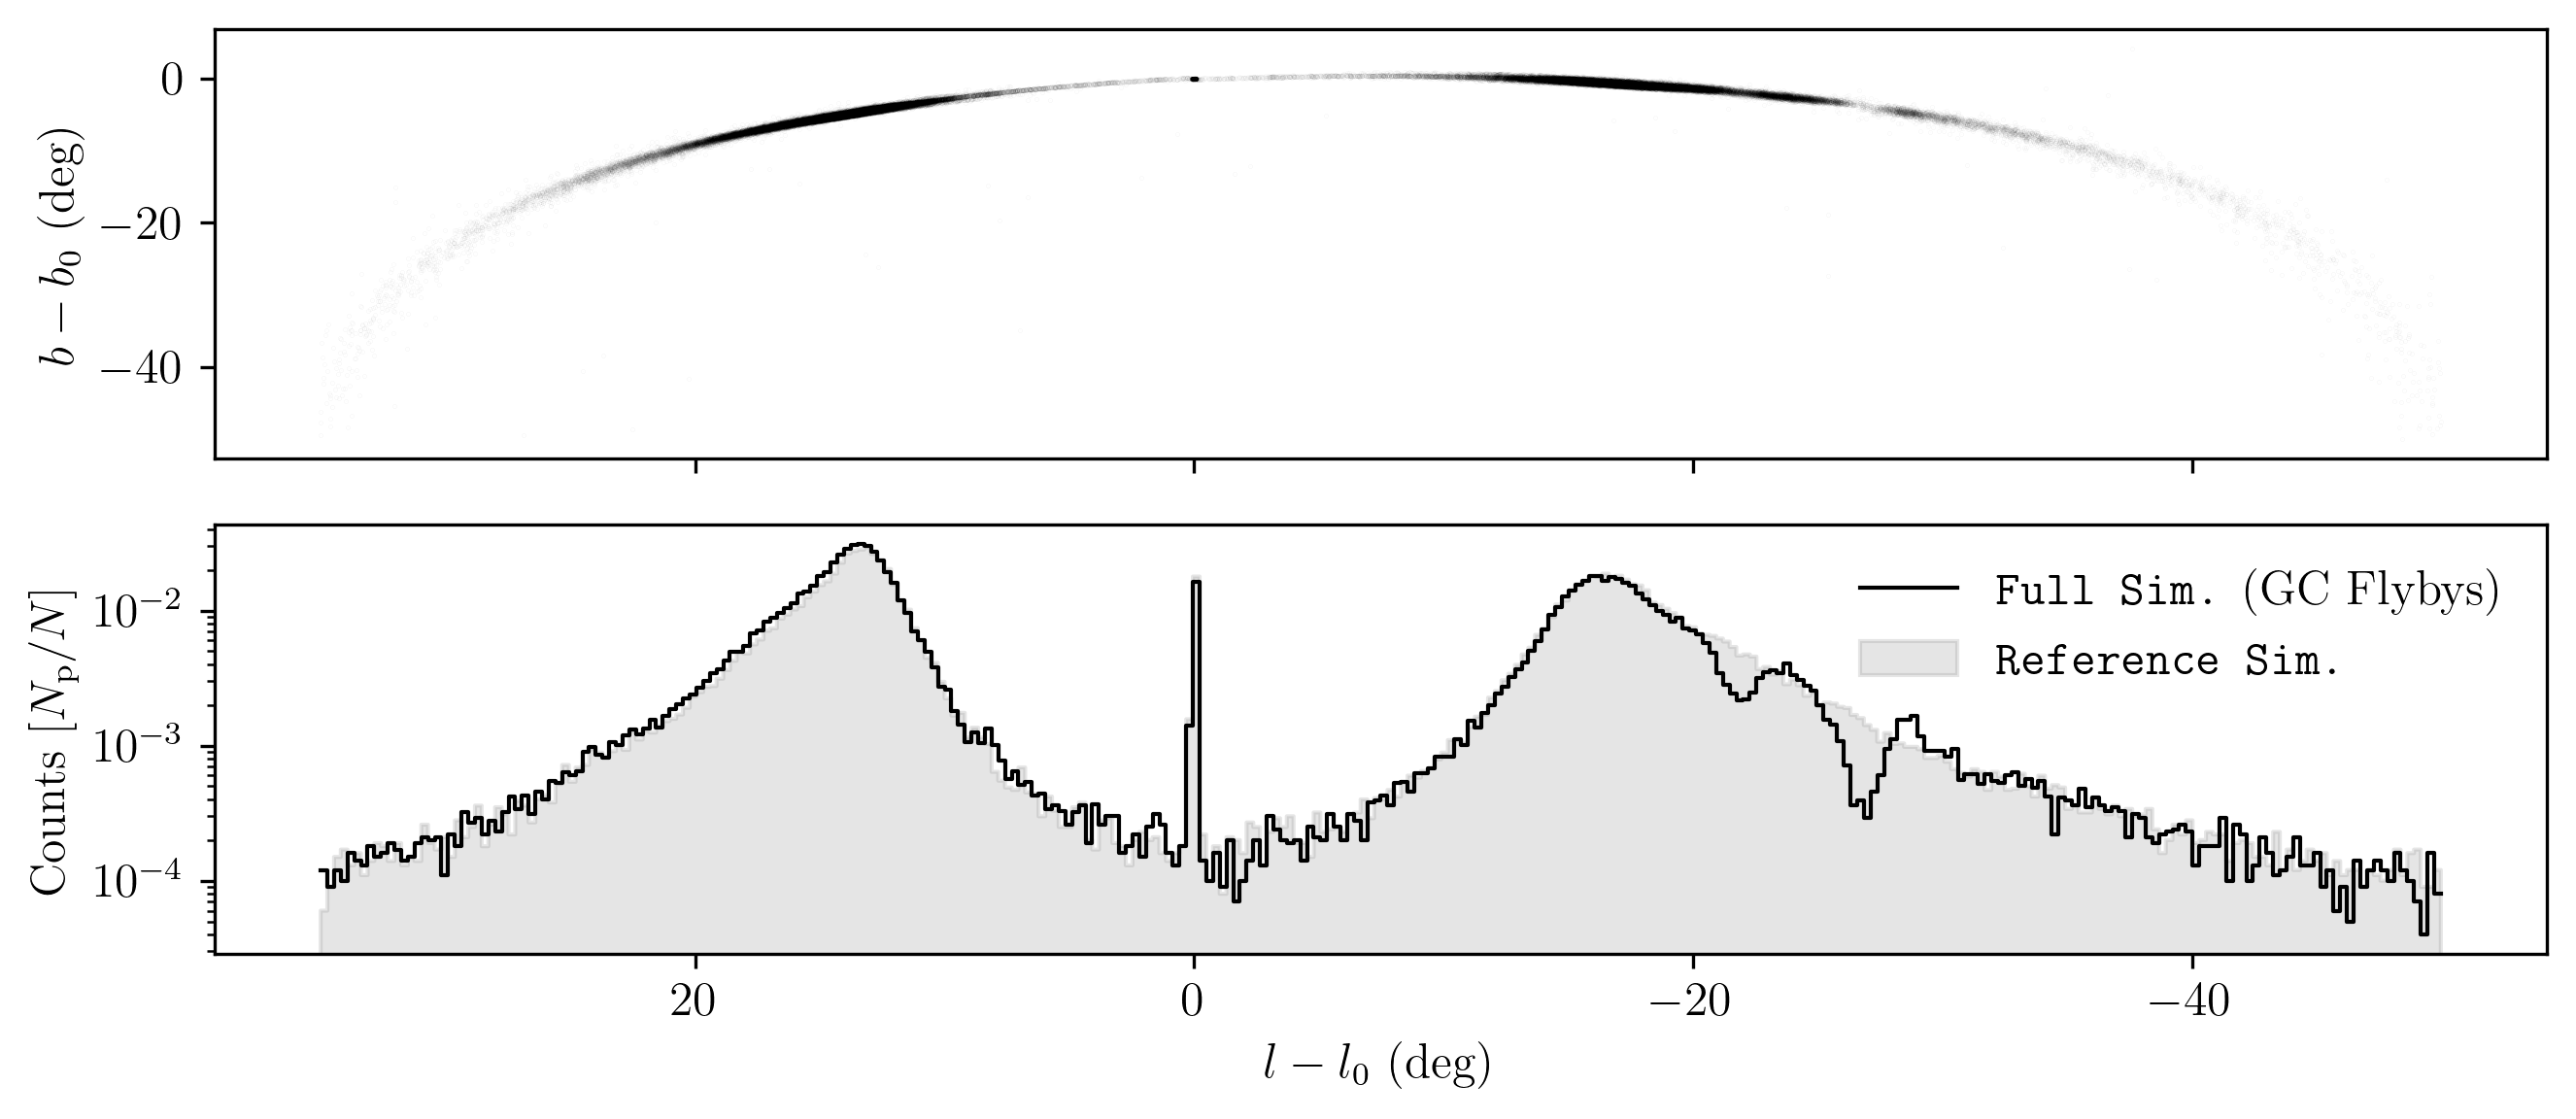
\includegraphics[width=\linewidth]{stream_on_sky_Pal5_monte-carlo-009_pouliasis2017pii-GCNBody_pouliasis2017pii.png}
    \caption{Simulated Palomar~5 stream created by modeling the host cluster as a Plummer sphere disrupting within an axis-symmetric Galactic potential plus the gravitational effect of 164 other galactic globular clusters. The top panel shows the distribution of \DIFdelbeginFL \DIFdelFL{star-particles }\DIFdelendFL \DIFaddbeginFL \DIFaddFL{star particles }\DIFaddendFL that escaped the cluster due to tidal forces. The bottom panel shows the 1D density profile marginalized over longitude. The gray fill shows a reference simulation \DIFdelbeginFL \DIFdelFL{where }\DIFdelendFL \DIFaddbeginFL \DIFaddFL{that uses }\DIFaddendFL the same conditions to produce the stream \DIFdelbeginFL \DIFdelFL{are used }\DIFdelendFL but \DIFaddbeginFL \DIFaddFL{does not include }\DIFaddendFL the \DIFdelbeginFL \DIFdelFL{effect of }\DIFdelendFL other globular clusters\DIFdelbeginFL \DIFdelFL{are not included}\DIFdelendFL . The large central peak in density \DIFdelbeginFL \DIFdelFL{are }\DIFdelendFL \DIFaddbeginFL \DIFaddFL{is }\DIFaddendFL of the particles still bound to Palomar~5. $\ell_0,b_0$ are located Palomar~5's cluster's center of mass. Two large gaps are present \DIFdelbeginFL \DIFdelFL{and are }\DIFdelendFL due to the passage of two globular clusters. $N_p$ indicates the number of particles in a bin\DIFaddbeginFL \DIFaddFL{, }\DIFaddendFL while $N$ is the total number of particles\DIFaddbeginFL \DIFaddFL{, }\DIFaddendFL which is 100,000.}
    \label{fig:stream_on_sky}
    \end{figure*}


\section{Methods}
  The most accurate model of the Palomar~5 stream would involve full modeling of the internal dynamics of the cluster\DIFdelbegin \DIFdel{. This }\DIFdelend \DIFaddbegin \DIFadd{, which }\DIFaddend would mean computing $N$-body interactions with a $\mathcal{O}(N^2)$ computation time, stellar evolution, supernovae, an initial mass distribution, treatment of binary star systems, etc. \citep[for such an example, see][]{2021NatAs...5..957G, 2016MNRAS.458.1450W}. Instead, we opt for solving the \textit{restricted-three body problem}, or as known as the \texttt{particle-test method} as we did for \citet{2023A&A...673A..44F}, which we describe here for completeness. As demonstrated by \citet{2012A&A...546L...7M}, although the restricted three-body problem neglects the internal evolution of the cluster, it still reproduces very similar stream properties \DIFdelbegin \DIFdel{. This is because }\DIFdelend \DIFaddbegin \DIFadd{since }\DIFaddend the model captures key extra-cluster physics, such as disk shocking and epicyclic stripping.\DIFaddbegin \\
  \DIFadd{Below, we first present the approach used to include the Galactic globular cluster system in our modeling (Sect.~\ref{numerical_meth}), highlighting the similarities and differences with respect to what we did in \mbox{%DIFAUXCMD
\citet{2023A&A...673A..44F}}\hskip0pt%DIFAUXCMD
; we then summarize the method used to model the mass loss from the cluster (Sect.~\ref{sec:mass_loss}) and finally discuss the quality of the numerical integration (Sect.~\ref{num_quality}). 
}\DIFaddend 

  \subsection{Numerical Methodology}\DIFaddbegin \label{numerical_meth}
    \DIFaddend We begin by extracting positions in the sky, proper motions, line-of-sight velocities\DIFaddbegin \DIFadd{, }\DIFaddend and distances, as well as masses and half-mass radii, of 165 globular clusters from the Galactic globular cluster catalog by \cite{2021MNRAS.505.5957B}.\footnote{The Baumgardt catalog has been assembled across a series of works, see: \cite{2020PASA...37...46B,2019MNRAS.482.5138B,2018MNRAS.478.1520B}. The catalog can be found on the World Wide Web at \href{https://people.smp.uq.edu.au/HolgerBaumgardt/globular/}{https://people.smp.uq.edu.au/HolgerBaumgardt/globular/}.} We then convert the initial conditions from sky coordinates into a Galactocentric reference frame, by adopting a velocity for the local standard of rest of $v_{\text{LSR}} = 240$~km~s$^{-1}$ and a peculiar velocity of the Sun equal to $(U_\odot, V_\odot, W_\odot)=(11.1, 12.24, 7.25)$~km~s$^{-1}$, as reported by \citet{2012MNRAS.427..274S}.  \DIFdelbegin \DIFdel{The position of the Sunwas set }\DIFdelend \DIFaddbegin \DIFadd{We set the Sun's position }\DIFaddend to $(x_\odot,y_\odot,z_\odot) = (-8.34,0,0.027)$~kpc\DIFdelbegin \DIFdel{, }\DIFdelend \DIFaddbegin \DIFadd{. We took the }\DIFaddend vertical position above the disk \DIFdelbegin \DIFdel{was taken }\DIFdelend from \citet{2001ApJ...553..184C} and the distance of the Sun to the Galactic center \DIFdelbegin \DIFdel{was taken }\DIFdelend from \citet{2014ApJ...783..130R}. These transformations were performed using \texttt{astropy} \citep{2013A&A...558A..33A}.

    For the Galactic potential, we used the second model from \citet{2017A&A...598A..66P}, a superposition of a thin disk, thick disk, and dark matter halo, with masses and scale lengths provided in Table~1 of \citet{2023A&A...673A..44F}. This model is time-independent throughout our simulations. This model satisfies a series of observational constraints such as local solar\DIFaddbegin \DIFadd{, }\DIFaddend stellar density, the Galactic rotation curve, etc., similarly to other Galactic models such as \texttt{MWpotential2014} from \citet{2015ApJS..216...29B} and \texttt{McMillian2017} from \citet{2017MNRAS.465...76M}. However, \DIFaddbegin \DIFadd{we use only one Galactic potential }\DIFaddend to balance data volume and computation time, \DIFdelbegin \DIFdel{we use only one Galactic potential, }\DIFdelend which should suffice. \citet{2021MNRAS.505.5978V} found that only a few outer globular clusters are strongly affected by different potential models. Generally, kinematic uncertainties are the dominant factor in differences between orbital solutions per cluster. Similarly, \citet{2024MNRAS.528.5189G} generated a globular cluster mass-loss catalog using seven different potential models and found their debris distributions to be rather model-independent, \DIFdelbegin \DIFdel{similarly }\DIFdelend \DIFaddbegin \DIFadd{similar }\DIFaddend to \citet{2023A&A...673A..44F}. While the clusters' exact positions in time may depend on the model, we assert that interaction rates and stream formation are largely independent \DIFaddbegin \DIFadd{of }\DIFaddend the choice of \DIFaddbegin \DIFadd{the }\DIFaddend Galactic potential model.

    Lastly, we select an integration time of 5~Gyr as a compromise between maximizing interaction statistics and \DIFdelbegin \DIFdel{adhering to the assumption that the galaxy can be modeled }\DIFdelend \DIFaddbegin \DIFadd{modeling the galaxy }\DIFaddend as a time-independent, constant mass distribution. \citet{2023A&A...673A.152I} analyzed the orbits of the Galactic cluster population using the same initial conditions as in this work \DIFdelbegin \DIFdel{, }\DIFdelend within five live Milky Way-like potentials from IllustrisTNG \citep{2018MNRAS.473.4077P}. They found that in all sampled potentials, orbital changes remain minimal over 5~Gyr, becoming significant only at earlier look-back times when the host galaxy had \DIFdelbegin \DIFdel{either }\DIFdelend significantly less mass or was undergoing a merger event.


    \subsubsection*{ \texttt{Full} simulations}
    There is a primary methodological departure from \citet{2023A&A...673A..44F}.  In that work, globular clusters evolved under the gravitational effect of the Galaxy only, while now we \DIFdelbegin \DIFdel{include also }\DIFdelend \DIFaddbegin \DIFadd{also include }\DIFaddend the effect of all the other Galactic globular clusters \DIFdelbegin \DIFdel{, by taking into account }\DIFdelend \DIFaddbegin \DIFadd{by considering }\DIFaddend the direct $N$-body interactions \DIFdelbegin \DIFdel{among them. To quantify these interactions}\DIFdelend \DIFaddbegin \DIFadd{between them. First}\DIFaddend , all clusters are represented by Plummer spheres, each with \DIFaddbegin \DIFadd{its own }\DIFaddend mass and half-mass \DIFdelbegin \DIFdel{radii }\DIFdelend \DIFaddbegin \DIFadd{radius }\DIFaddend as reported in the Baumgardt catalog \citep{2021MNRAS.505.5957B}. For the remainder of this paper, \DIFdelbegin \DIFdel{we refer to these simulations , where the globular clusters interactionsare taken into account as }\texttt{\DIFdel{full}} %DIFAUXCMD
\DIFdel{simulations}\DIFdelend \DIFaddbegin \DIFadd{the }\texttt{\DIFadd{full}} \DIFadd{simulations consider the gravitational forces from the globular cluster interactions}\DIFaddend . \\
    For these simulations, we proceed \DIFdelbegin \DIFdel{into }\DIFdelend \DIFaddbegin \DIFadd{in }\DIFaddend two steps:
      \begin{enumerate}
          \item First, starting from the Galactocentric positions and velocities of all 165 Galactic globular clusters, we integrate their orbits back in time for 5~Gyr under the influence of the Galaxy itself and their mutual influence. In the backward integration, the system of equations of motion for the globular clusters \DIFdelbegin \DIFdel{are thus: 
          }\DIFdelend \DIFaddbegin \DIFadd{is thus: 
          }\DIFaddend \begin{equation}
          \ddot{\vec{r}}_i = -\nabla \Phi \DIFdelbegin \DIFdel{(R_i,z_i) }\DIFdelend + \left.\sum_{j\neq i}^{N_{GC}} \frac{Gm_j}{\left(|\vec{r}_j - \vec{r}_i|^2 + b_j^2\right)^{3/2}}\right. \left(\vec{r}_j - \vec{r}_i\right),
          \end{equation}\label{eq:GCNBody} 
          \noindent where $\vec{r}$ indicates the galactocentric position vector, the index $i$ indicates the globular cluster of interest\DIFdelbegin \DIFdel{with $R_i,z_i$ being its galactocentric positions in cylindrical coordinates}\DIFdelend ; the index $j$ indicates the other globular clusters that are summed over. $N_{GC}$ is the total number of globular clusters\DIFaddbegin \DIFadd{, }\DIFaddend which in this study is 165, $m_j$ is the mass of the j-th cluster in the sample, $b_j$ is its Plummer scale radius, and $\vec{r_j}$ is its galactocentric position. $\Phi$ represents the same Galactic smooth potential that we discussed previously\citep[][Model~II, in the present case]{2017A&A...598A..66P}. Note that the masses and sizes of the globular clusters are kept constant in these simulations and \DIFaddbegin \DIFadd{are }\DIFaddend not allowed to vary with time\DIFdelbegin \DIFdel{. This equally implies }\DIFdelend \DIFaddbegin \DIFadd{, which means }\DIFaddend that we do not \DIFdelbegin \DIFdel{take into account the internal evolutionof the globular clusters in these models. We }\DIFdelend \DIFaddbegin \DIFadd{consider their internal evolution. In the Discussion section, we }\DIFaddend discuss the implications of the modeling limitations\DIFdelbegin \DIFdel{in the Discussion}\DIFdelend .

        \item Once the \DIFaddbegin \DIFadd{we find the }\DIFaddend positions and velocities of the entire globular cluster system 5~Gyr ago\DIFdelbegin \DIFdel{are found}\DIFdelend , we sample Palomar~5 with 100,000 particles from a Plummer distribution\DIFaddbegin \DIFadd{, }\DIFaddend taking the mass and half-mass radius from the Baumgardt catalog\DIFaddbegin \DIFadd{: $1.3\times10^{4}~\textrm{M}_\odot$ \& $27.6~\textrm{pc}$}\DIFaddend . We then integrate the evolution of these particles forward in time to the present day \DIFdelbegin \DIFdel{, }\DIFdelend by taking into account that each particle feels the gravitational potential of the Galaxy, that of its host cluster, and that of all the other clusters in the Galaxy. Note that we do not take \DIFdelbegin \DIFdel{into account }\DIFdelend self-gravity among particles \DIFaddbegin \DIFadd{into account}\DIFaddend . The particles experience the gravitational field yet do not contribute to it, which is a common assumption made in Galactic dynamics since the mass of an individual star is negligible compared to the mass of the larger dynamical system. The equation of motion of a generic particle among the 100,000 \DIFdelbegin \DIFdel{which }\DIFdelend \DIFaddbegin \DIFadd{that }\DIFaddend populate Palomar~5 is thus: 
        \begin{equation}
          \ddot{\vec{r}}_p = -\nabla \Phi \DIFdelbegin \DIFdel{(R_p,z_p) }\DIFdelend + \left.\sum_{j}^{N_{GC}} \frac{Gm_j}{\left(|\vec{r}_j(t) - \vec{r}_p|^2 + b_j^2\right)^{3/2}}\right. \left(\vec{r}_j(t)- \vec{r}_p\right),
          \end{equation} \label{eq:equation_of_motion_particle} where the index $p$ represents one of the 100,000 particles of interest, $\vec{r_p}$ being its position, and $j$ indexes over the globular clusters as in Eq.~\ref{eq:GCNBody}. Note that in Eq.~\ref{eq:equation_of_motion_particle}\DIFaddbegin \DIFadd{, }\DIFaddend the positions of the globular clusters are time-dependent since they are being loaded during this step and not computed, unlike Eq.~\ref{eq:GCNBody}. 

      \end{enumerate}




        The procedure described so far has been repeated 50 times, \DIFdelbegin \DIFdel{each time }\DIFdelend generating a new set of initial conditions \DIFaddbegin \DIFadd{each time}\DIFaddend , given the uncertainties on proper motions, line-of-sight velocities, distances to the Sun, and masses \DIFdelbegin \DIFdel{, }\DIFdelend of all clusters, as reported in the Baumgardt catalog. We handle these uncertainties through a Monte-Carlo approach \DIFdelbegin \DIFdel{, }\DIFdelend by sampling them with a Gaussian distribution \DIFdelbegin \DIFdel{, and by taking into account }\DIFdelend \DIFaddbegin \DIFadd{and considering }\DIFaddend the covariance term between the proper motions. \DIFdelbegin \DIFdel{For the first simulation, we }\DIFdelend \DIFaddbegin \DIFadd{We }\DIFaddend use the most probable values for the initial conditions \DIFdelbegin \DIFdel{. The uncertainties are sampled }\DIFdelend \DIFaddbegin \DIFadd{in the first simulation. We sample the uncertainties }\DIFaddend for all globular clusters. Additionally, for each \DIFdelbegin \DIFdel{re-sampling }\DIFdelend \DIFaddbegin \DIFadd{resampling }\DIFaddend of Palomar~5's mass, we also resample the distribution of the 100,000 \DIFdelbegin \DIFdel{star-particles}\DIFdelend \DIFaddbegin \DIFadd{star particles}\DIFaddend . 


      During the integration, \DIFdelbegin \DIFdel{intermediate snapshots were saved }\DIFdelend \DIFaddbegin \DIFadd{we save intermediate snapshots }\DIFaddend to facilitate the analysis of stellar streams and the effects of cluster impacts. Specifically, for each \DIFdelbegin \DIFdel{of the 50 realizations of the }\DIFdelend \DIFaddbegin \DIFadd{realization of the }\DIFaddend Palomar~5 stream, we saved $5000$ \DIFdelbegin \DIFdel{intermediate time-steps which is }\DIFdelend \DIFaddbegin \DIFadd{in snapshots, equivalent to }\DIFaddend a temporal resolution of 1 million years. We provide the parameters that specify our data volume in Table~\ref{tab:data_volume}. Using single precision floating point numbers, the size of our simulations is approximately:
    \begin{equation} \label{eq:data_volume_estimate}
      N_p \times N_{\textrm{ts}}\times N_{\textrm{phase}}\times N_{\textrm{sampling}} \times 4~\textrm{bytes}\approx 600~\textrm{Gb}.
    \end{equation}

    \begin{table}[h]
      \centering
      \begin{tabular}{|c|c|c|c|}
          \hline
          $N_p$ & $N_{\textrm{ts}}$ & $N_{\textrm{phase}}$ & $N_{\textrm{sampling}}$ \\
          \hline
          $100000$ & $5000$ & $6$ & $50$ \\
          \hline
      \end{tabular}
      \caption{The parameters determining the data volume of this experiment. where $N_p$  is the number of particles, $N_{\textrm{ts}}$ is the number of time-steps saved, $N_{\textrm{phase}}$ is the number of phase space coordinates, and $N_{\textrm{sampling}}$ is the number of Monte-Carlo samplings of the initial conditions.}
      \label{tab:data_volume}
    \end{table}

  \subsubsection*{ \texttt{Reference} simulations}

    To quantify the impact of globular cluster passages \DIFdelbegin \DIFdel{to }\DIFdelend \DIFaddbegin \DIFadd{on }\DIFaddend the density of \DIFaddbegin \DIFadd{the }\DIFaddend Palomar~5 stream, we performed a second set of simulations, which we refer to as the \texttt{reference} simulations in this paper.  These \texttt{reference} simulations use the same 50 sets of initial conditions as the \texttt{full} simulations, the same Galactic potential\DIFaddbegin \DIFadd{, }\DIFaddend but exclude mutual interactions between globular clusters. The approach adopted for this second set of simulations is thus equivalent to that adopted already in \citet{2023A&A...673A..44F}. In Eq.~\ref{eq:GCNBody}\DIFaddbegin \DIFadd{, }\DIFaddend only the gradient of the Galactic potential is considered. In Eq.~\ref{eq:equation_of_motion_particle}, of the second term on the \DIFdelbegin \DIFdel{right-side }\DIFdelend \DIFaddbegin \DIFadd{right side }\DIFaddend of the equation, only the influence of Palomar~5's Plummer sphere on Palomar~5's particles is considered. In other words, \DIFaddbegin \DIFadd{the }\DIFaddend sum iterates over only one globular cluster, the host. \DIFdelbegin \DIFdel{All the }\DIFdelend \DIFaddbegin \DIFadd{We omit all }\DIFaddend interactions with the other clusters\DIFdelbegin \DIFdel{in the Galaxy are indeed omitted. }\DIFdelend \DIFaddbegin \DIFadd{.
}\DIFaddend 

\DIFdelbegin \subsubsection*{\DIFdel{Numerical Stability}}
%DIFAUXCMD
%DIFDELCMD < 

%DIFDELCMD <     %%%
\DIFdel{The integration was conducted using a leapfrog integrator, chosen for }\DIFdelend \DIFaddbegin \subsection{\DIFadd{Mass loss}}\label{sec:mass_loss}

\DIFadd{Each of the 100,000 particles that initially populate the cluster undergoes, over time, acceleration due to the Pal~5 potential, whose mass and half-mass radius we assume to be fixed over time, and to the Galactic potential. At each time step, a certain number of particles will therefore acquire sufficient energy to no longer be gravitationally bound to the cluster itself and thus go on to populate the streams, whose mass and spatial extent grow over time. It is important to note that in the approach used:
}

\begin{enumerate}
    \item \DIFadd{The masses and sizes of the clusters (and therefore the parameters of the Plummer potentials) do not change over time, which is a blatant simplification, because in a self-consistent approach, these parameters would vary. 
    }\item \DIFadd{We use the same initial conditions for Pal~5 progenitor as it has today, and this is also a simplification, since Pal~5 - 5 Gyr years ago - must have contained at least part of the mass estimated today in its tails}\footnote{\DIFadd{We use the same approach (i.e. time-independent masses and sizes) to model the whole set of globular clusters.}}\DIFadd{. 
}\end{enumerate}

\DIFadd{The assumption in point 2 is a direct consequence of the approach described in point 1. Starting from a cluster with mass and size similar to the current ones can lead to streams with lower velocity dispersions than those we would have obtained if we had used a self-consistent approach. In a future article, we will report on the study of gap survival times depending on the masses and sizes of progenitor clusters (Ferrone et al, in prep). We note, however, that simplifications of this kind are not uncommon in literature. \mbox{%DIFAUXCMD
\citet{2017NatAs...1..633P} }\hskip0pt%DIFAUXCMD
discussed the formation of gaps in the Pal~5 tails and assumed a time-independent mass of $50,000 ~\textrm{M}_\odot$ for Pal~5, over the last 4~Gyr; \mbox{%DIFAUXCMD
\citet{2017MNRAS.470...60E} }\hskip0pt%DIFAUXCMD
adopted a N-body approach to simulate Pal~5 stream, but used Pal~5 current conditions as their progenitor's initial conditions; \mbox{%DIFAUXCMD
\citet{2019MNRAS.484.2009B} }\hskip0pt%DIFAUXCMD
simulated the Pal~5 stream as emerging from a stellar system with a velocity dispersion of 0.5~km/s (similar to that of particles escaping from our cluster, as we have verified). 
}

\DIFadd{The characteristics of the streams modeled in this paper may be considered more representative of those of clusters that are now completely dispersed, i.e. it is conceivable that completely dispersed globular clusters that left behind a population of `orphan' streams passed through characteristics similar to those of Pal~5 today (small masses and extended radii). In this sense, the initial conditions chosen (in terms of internal parameters) could be considered more representative of those of streams found in the Galaxy and for which the progenitor is now dissolved \mbox{%DIFAUXCMD
\citep[see, for example, the population of streams without progenitors described by][]{2024ApJ...967...89I} }\hskip0pt%DIFAUXCMD
than those currently typical of Galactic globular clusters}\footnote{\DIFadd{In this regard, we recall that \mbox{%DIFAUXCMD
\citet{2014ApJ...795...95B} }\hskip0pt%DIFAUXCMD
modeled the GD-1 stream as the result of the dissolution of a cluster with a mass of $2 \times 10^4 M_\odot$, and a tidal radius of $0.07$~kpc.}}




  \subsection{\DIFadd{Numerical Stability}}\label{num_quality}

    \DIFadd{We used a leapfrog integrator because of }\DIFaddend its ability to preserve phase-space volume and conserve the Hamiltonian with each integration step. \DIFdelbegin \DIFdel{This }\DIFdelend \DIFaddbegin \DIFadd{For instance, this }\DIFaddend method is preferable to \DIFdelbegin \DIFdel{, for instance, }\DIFdelend a Runge-Kutta scheme, which can introduce non-physical and significant numerical errors in systems that require long-term stability and energy conservation. One drawback of the leapfrog integrator is that it requires a uniform \DIFdelbegin \DIFdel{time-step }\DIFdelend \DIFaddbegin \DIFadd{time step }\DIFaddend across the entire computation, leading to unnecessary computations for a particle after it escapes \DIFdelbegin \DIFdel{form }\DIFdelend \DIFaddbegin \DIFadd{from }\DIFaddend the host cluster. However, energy conservation and phase-space volume preservation are paramount when modeling stellar streams. The time step was\DIFdelbegin \DIFdel{therefore }\DIFdelend \DIFaddbegin \DIFadd{, therefore, }\DIFaddend set to be small enough to conserve energy for the most interior particles within the cluster---ensuring that a higher mass loss did not arise from numerical error. \DIFdelbegin \DIFdel{For these simulations, }\DIFdelend \DIFaddbegin \DIFadd{We found that }\DIFaddend a time-step of 10,000 years was \DIFdelbegin \DIFdel{selected to maintain adequate }\DIFdelend \DIFaddbegin \DIFadd{adequate to maintain }\DIFaddend energy conservation, with a median variation of $10^{-12} \frac{\Delta E}{E_0}$, where $E_0$ is a particle's initial energy, and $\Delta E$ is the difference between its final and initial energy. 

    We also checked the \textit{reverse integrability} of the globular cluster system for the \texttt{reference} simulations. By reverse integrability, we mean the integrator's capability to track the cluster backward in time and then re-integrate it forward along the same trajectory. Integrating point masses in a static axis-symmetric potential conserves $L_z$ and $E$, which create regular periodic and non-chaotic orbits. Therefore, any drift would arise from purely numerical error. We selected a \DIFdelbegin \DIFdel{time stamp }\DIFdelend \DIFaddbegin \DIFadd{timestamp }\DIFaddend for which the drift in the final position after forward integration, compared to the initial position from the backward integration, was consistently at least two orders of magnitude smaller than the Plummer scale radius used for Palomar~5. This high precision ensures that no fictitious numerical forces \DIFdelbegin \DIFdel{influenced }\DIFdelend \DIFaddbegin \DIFadd{influence }\DIFaddend the system, preventing any artificial mass loss or retention of star particles.

\section{Results}



  \subsection{Overview}

    \begin{figure*}
      \centering
      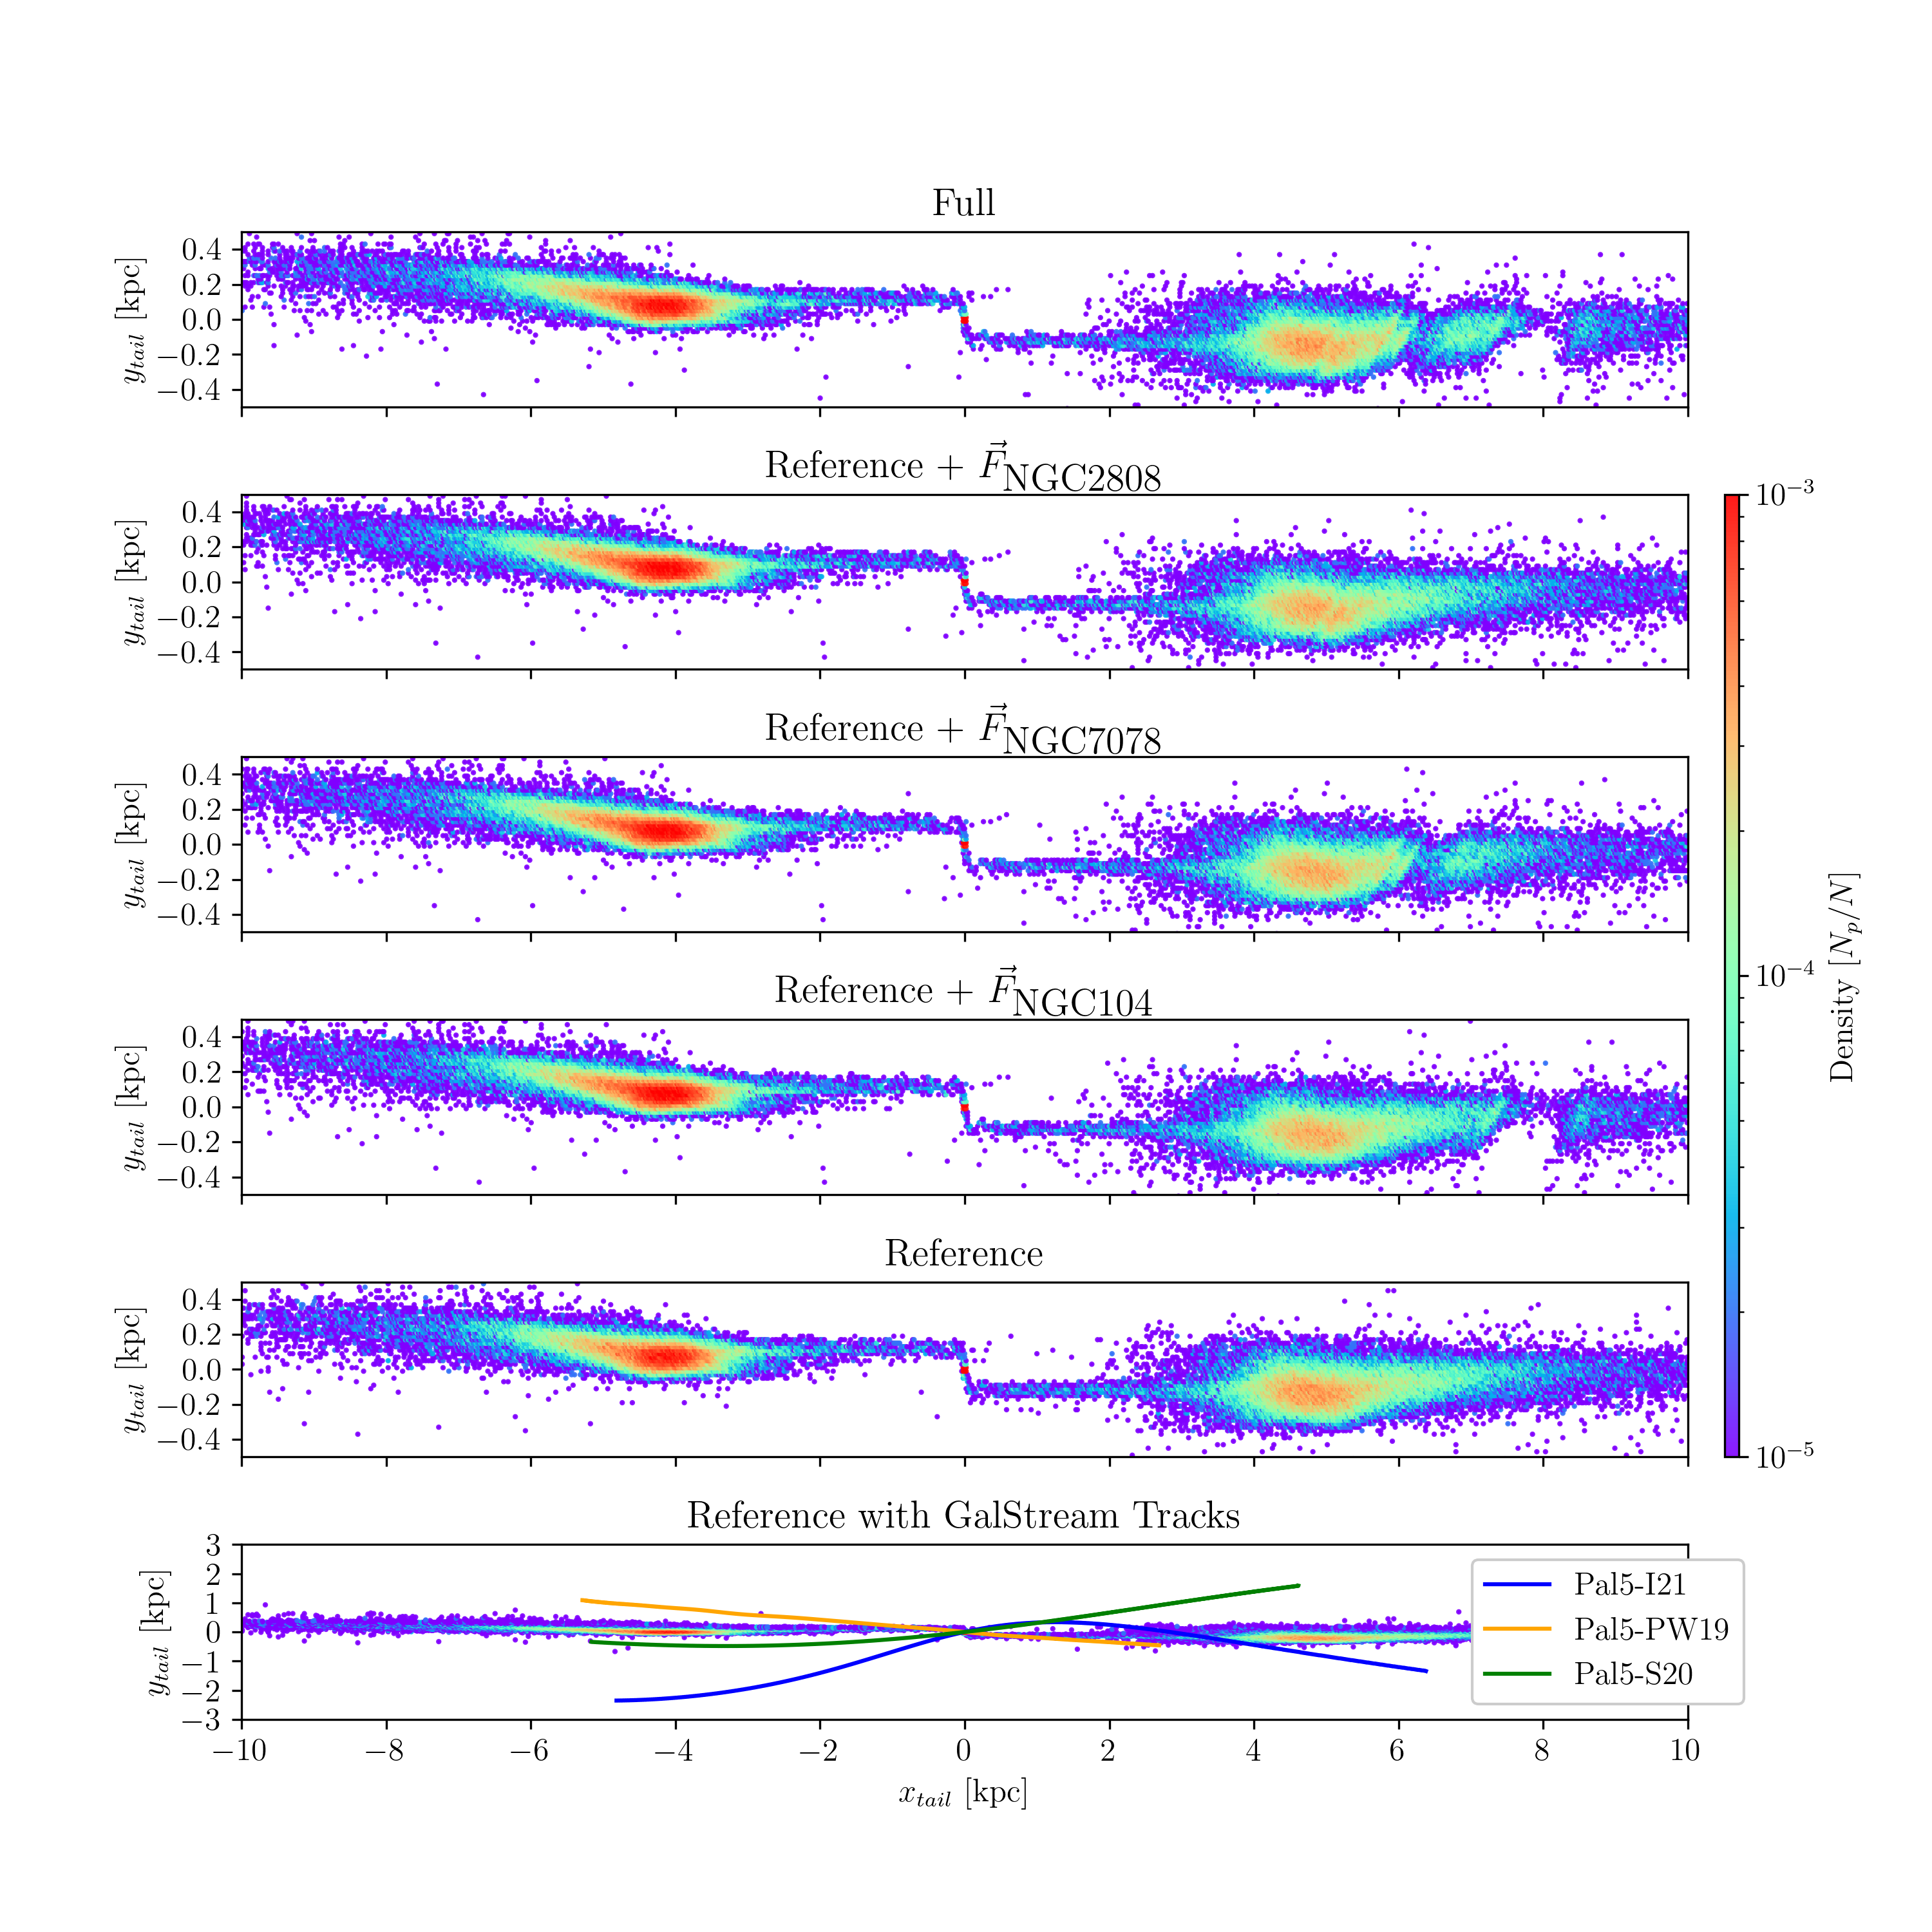
\includegraphics[width=\linewidth]{decomposition-monte-carlo-009-with-3-gaps-domidpoint-shift.png}
      \caption{Density maps of Palomar~5's stream in the tail coordinate system\DIFaddbeginFL \DIFaddFL{, where $x\prime$ is the integrate arclength along the cluster's orbit and $y\prime$ is the distance within the orbital plane}\DIFaddendFL . The color scale represents normalized particle counts (total: 100,000). The top panel shows the \texttt{full} simulation with three gaps on the stream's right-hand side. The next three panels depict simulations with identical initial conditions but exclude the gravitational influence of all clusters except those forming a given gap. The \texttt{Reference} simulation omits the influence from other globular clusters. The bottom panel compares Palomar~5's observed stream length to the \texttt{Reference} simulation, using the same Monte Carlo realization as Fig.~\ref{fig:stream_on_sky} and \texttt{Sampling~009} of Fig.~\ref{fig:gallery2}.}
      \label{fig:decomposition}
    \end{figure*} 

    \begin{figure*}
      \centering
      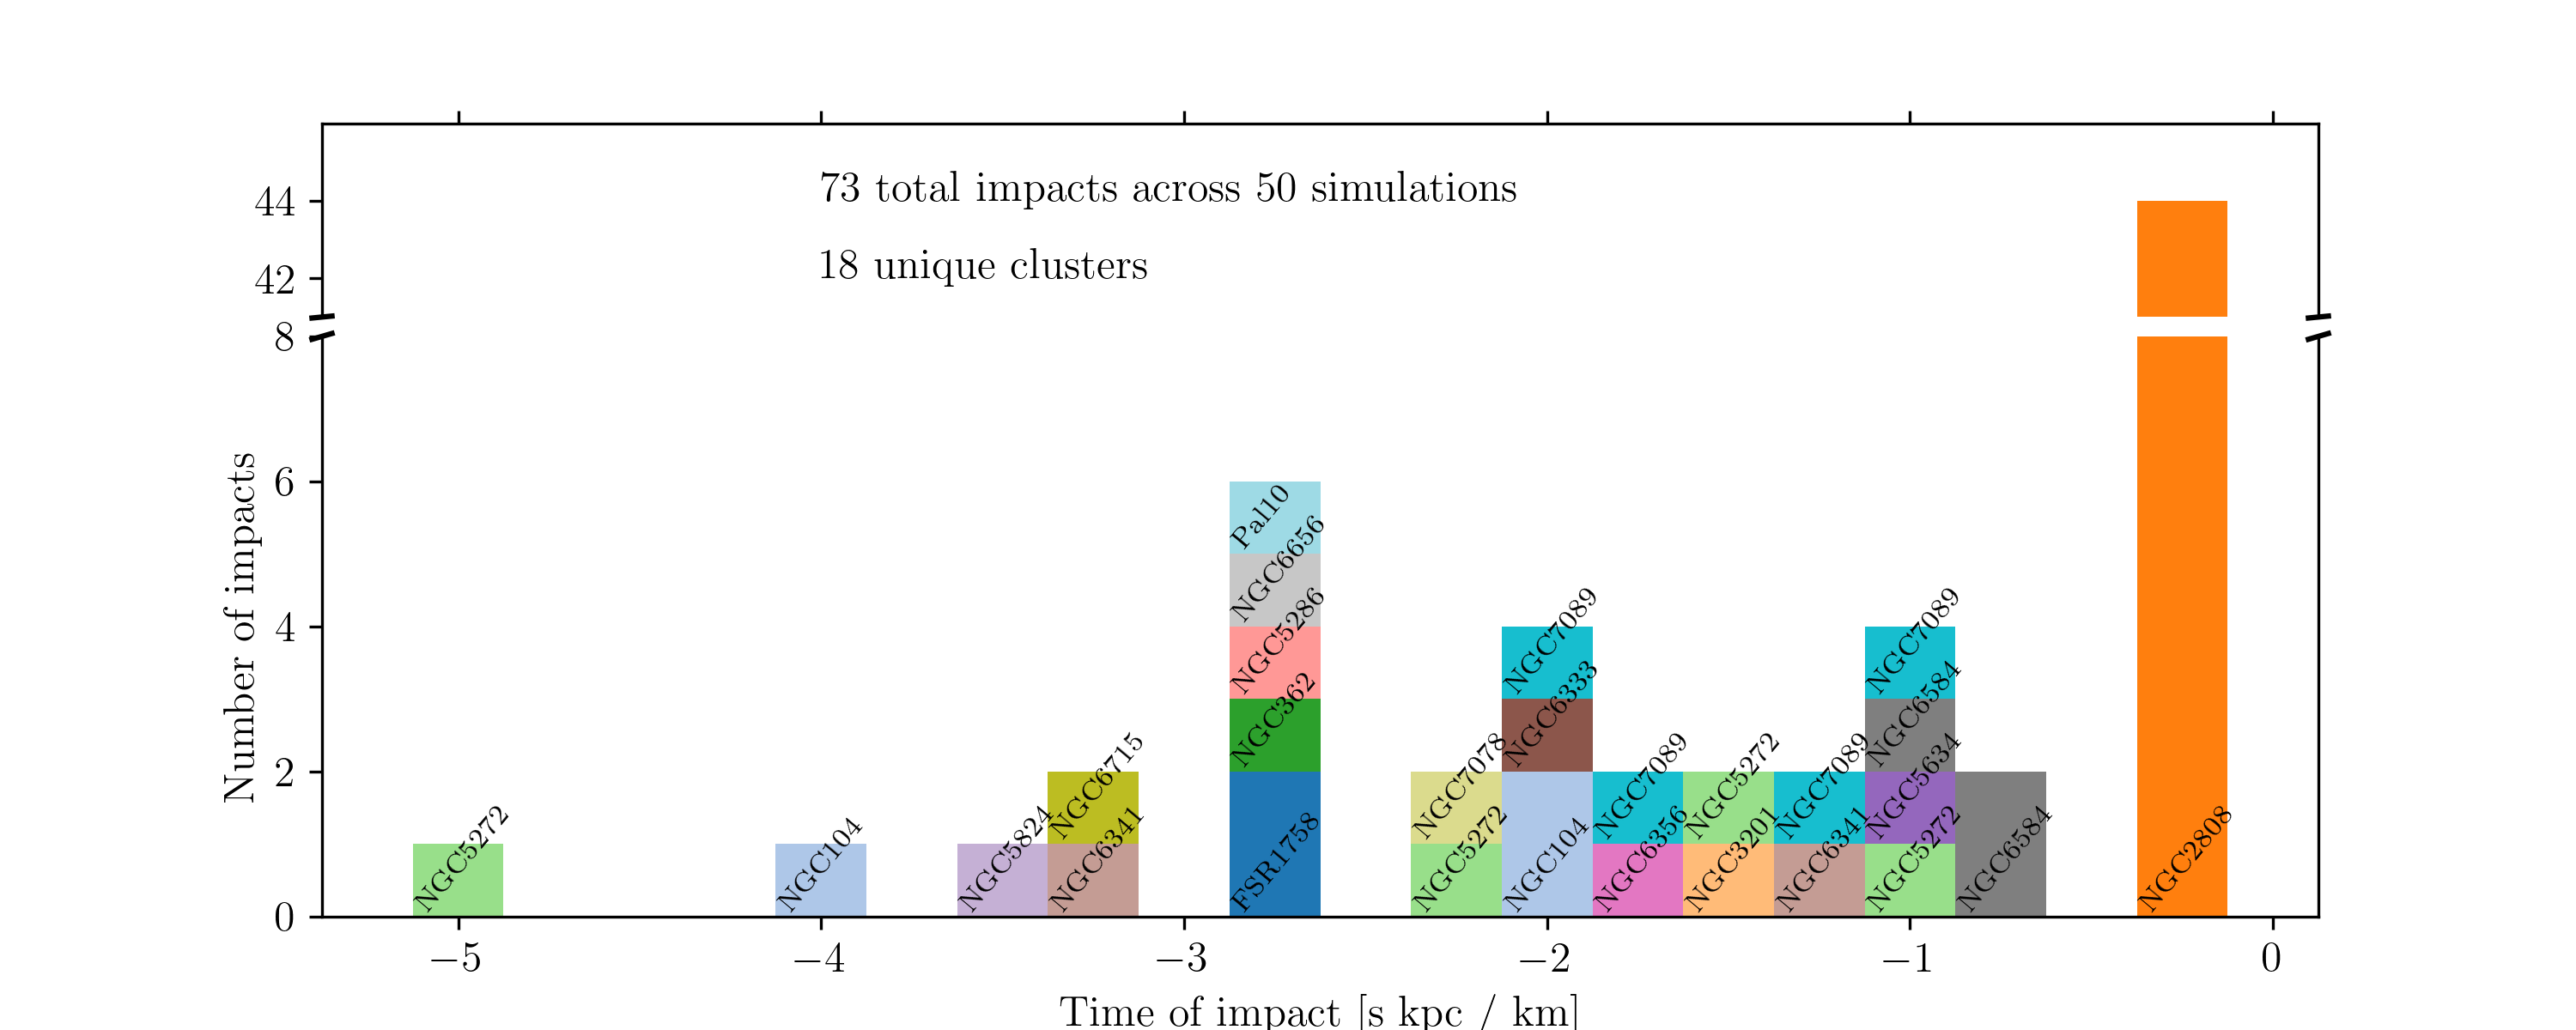
\includegraphics[width=\linewidth]{histogram_impact_time.png}
      \caption{The simulation time \DIFdelbeginFL \DIFdelFL{at which }\DIFdelendFL \DIFaddbeginFL \DIFaddFL{when }\DIFaddendFL the impacts occurred for all \DIFdelbeginFL \DIFdelFL{gap causing }\DIFdelendFL \DIFaddbeginFL \DIFaddFL{gap-causing }\DIFaddendFL flybys summed over all 50 simulations. Each perturbing cluster is \DIFdelbeginFL \DIFdelFL{label }\DIFdelendFL \DIFaddbeginFL \DIFaddFL{labeled }\DIFaddendFL and \DIFdelbeginFL \DIFdelFL{is color consistent}\DIFdelendFL \DIFaddbeginFL \DIFaddFL{color-consistent}\DIFaddendFL . \DIFdelbeginFL \DIFdelFL{The }\DIFdelendFL \DIFaddbeginFL \DIFaddFL{We report the }\DIFaddendFL time axis \DIFdelbeginFL \DIFdelFL{is given }\DIFdelendFL in simulation units, with 1~s~kpc~km~$^{-1}$ corresponding to roughly 1~Gyr. Note that the \DIFaddbeginFL \DIFaddFL{plot breaks the }\DIFaddendFL y-axis \DIFdelbeginFL \DIFdelFL{is broken }\DIFdelendFL to accommodate the large number of encounters from \DIFdelbeginFL \DIFdelFL{NGC2808, }\DIFdelendFL \DIFaddbeginFL \DIFaddFL{NGC~2808 }\DIFaddendFL without overshadowing the other interactions.}
      \label{fig:histogram_impact_time}
    \end{figure*}


    
    %DIF <  To our knowledge, this is the first study to investigate the gravitational interactions between all Galactic globular clusters. While we did not  observe significant changes to orbital properties of the clusters, when subject to their mutual interactions -- a result which is  expected given the small sizes and vast distances between the clusters -- we do 
    %DIF <  This is no longer true after Sergey showed me the papers from Ischenko et al for the globular cluster ineractions
    \DIFdelbegin %DIFDELCMD < 

%DIFDELCMD <     %%%
\DIFdelend The presence of the other globular clusters \DIFdelbegin \DIFdel{has a clear effect on }\DIFdelend \DIFaddbegin \DIFadd{affects }\DIFaddend the properties of \DIFaddbegin \DIFadd{the }\DIFaddend Palomar~5 stream. \DIFdelbegin \DIFdel{A particularly clear example of this effect is shown in }\DIFdelend Fig.~\ref{fig:stream_on_sky} \DIFaddbegin \DIFadd{presents an obvious example of this effect, }\DIFaddend which we selected for its prominent gaps. Two of these gaps are \DIFdelbegin \DIFdel{clearly }\DIFdelend visible in Galactic coordinates and become even more apparent when marginalizing over latitude to reconstruct the 1D density profile of the stream \DIFdelbegin \DIFdel{, }\DIFdelend as a function of longitude.     

    Regarding the shape of the density distribution, the central peak corresponds to the still-intact globular cluster whose stars have not yet escaped. The \DIFdelbegin \DIFdel{density peaks in the stream are of }\DIFdelend \DIFaddbegin \DIFadd{stream's density peaks are }\DIFaddend the same order as the cluster itself\DIFdelbegin \DIFdel{. This }\DIFdelend \DIFaddbegin \DIFadd{, which }\DIFaddend is inconsistent with reality\DIFdelbegin \DIFdel{, }\DIFdelend \DIFaddbegin \DIFadd{; }\DIFaddend the cluster's peak density should be higher than the stream's\DIFdelbegin \DIFdel{peak density}\DIFdelend . Of course, this discrepancy is a result of our modeling choices. \DIFdelbegin \DIFdel{We use the present day }\DIFdelend \DIFaddbegin \DIFadd{Since we use the present-day }\DIFaddend mass and radius for Palomar~5 for the whole \DIFdelbegin \DIFdel{duration of the simulation. Consequently the system is modeled as being }\DIFdelend \DIFaddbegin \DIFadd{simulation duration, the system is }\DIFaddend less dense than it should have been. In turn, our simulations have a strong initial mass loss\DIFaddbegin \DIFadd{, }\DIFaddend which adds to the amplitudes of the profile density peaks of Fig.~\ref{fig:stream_on_sky}. This inaccuracy is acceptable for the scope of this work. First is that Palomar~5's tails indeed have more mass than the cluster itself. \citet{2017ApJ...842..120I} reports that there could be three times as much mass in Palomar~5's tails as the cluster itself. Secondly, the exact form of the density distribution is less important than having a population of particles present that can probe a cluster flyby event.

    To \DIFdelbegin \DIFdel{make a more quantitative comparison between }\DIFdelend \DIFaddbegin \DIFadd{compare }\DIFaddend the \texttt{reference} and \texttt{full} simulations \DIFaddbegin \DIFadd{more quantitatively}\DIFaddend , we work in the tail coordinate system, in which the stream\DIFdelbegin \DIFdel{is aligned }\DIFdelend \DIFaddbegin \DIFadd{'s central axis aligns }\DIFaddend with the cluster's orbit. \DIFdelbegin \DIFdel{The definition of }\DIFdelend \DIFaddbegin \DIFadd{We based }\DIFaddend this coordinate system \DIFdelbegin \DIFdel{is based }\DIFdelend on the work of \citet{2004AJ....127.2753D} and \DIFdelbegin \DIFdel{is shown }\DIFdelend \DIFaddbegin \DIFadd{present it }\DIFaddend in Fig.~\ref{fig:TailCoordinates}. Briefly, in this system\DIFaddbegin \DIFadd{, }\DIFaddend the $x_{\textrm{tail}}$ coordinate represents the position of a particle along the orbit relative to the globular cluster. Positive values of $x_{\textrm{tail}}$ are ahead of the cluster\DIFaddbegin \DIFadd{, }\DIFaddend while negative $x_{\textrm{tail}}$ is behind the cluster. The $y_{\textrm{tail}}$ coordinate measures the particle's distance within the orbital plane, where positive values indicate that the particle is farther from the Galactic center and negative values indicate that it is closer. Fig.~\ref{fig:decomposition} shows a comparison between one of the 50 realizations of \DIFaddbegin \DIFadd{the }\DIFaddend Palomar~5 stream\DIFaddbegin \DIFadd{, }\DIFaddend taking into account the gravitational interactions with all other globular clusters in the Galaxy (top panel) and omitting them (bottom panel). This comparison clearly shows the presence of two wide ($\sim$100~pc and $\sim$1~kpc) gaps in the leading tail and of a more subtle under-density at $x_{\textrm{tail}}\sim 5$~kpc (we refer the reader to Appendix~\ref{sec:gap_detection} for a detailed description of the under-densities and gaps detection method). 

    To find out which globular clusters were responsible \DIFdelbegin \DIFdel{of }\DIFdelend \DIFaddbegin \DIFadd{for }\DIFaddend creating these gaps \DIFdelbegin \DIFdel{, }\DIFdelend and when close passages took place, we estimated the gravitational acceleration along the orbit of Palomar~\DIFdelbegin \DIFdel{5 and }\DIFdelend \DIFaddbegin \DIFadd{5. We }\DIFaddend represented it in the ($t$, $\tau$) space. $t$ is the simulation time\DIFaddbegin \DIFadd{, }\DIFaddend and $\tau$ \DIFdelbegin \DIFdel{is }\DIFdelend indicates how long it will take for Palomar~5 to reach \DIFdelbegin \DIFdel{, }\DIFdelend \DIFaddbegin \DIFadd{a given point in its orbit }\DIFaddend or how long ago it passed\DIFdelbegin \DIFdel{, a given point on its orbit}\DIFdelend . The use of $\tau$ is advantageous because the growth of the stream is approximately linear in $\tau$. 
    On the other hand, \DIFaddbegin \DIFadd{streams }\DIFaddend in physical space \DIFdelbegin \DIFdel{streams on eccentric orbits indeed grow in time yet the growth rate is modulated }\DIFdelend \DIFaddbegin \DIFadd{grow linearly. Yet, their eccentricity modulates this growth }\DIFaddend with periodic expansion and contraction depending on the orbital phase \citep[see the top panel of Fig.~5.][for an example]{2016MNRAS.457.3817S}. Adopting this \DIFdelbegin \DIFdel{time space, }\DIFdelend \DIFaddbegin \DIFadd{time-space }\DIFaddend and reporting the gravitational acceleration along \DIFaddbegin \DIFadd{the }\DIFaddend Palomar~5 orbit in this space, \DIFdelbegin \DIFdel{the identification of the globular clusters which }\DIFdelend \DIFaddbegin \DIFadd{identifying the globular clusters that }\DIFaddend produced the perturbation \DIFdelbegin \DIFdel{, }\DIFdelend and the time \DIFdelbegin \DIFdel{at which }\DIFdelend it occurred becomes \DIFdelbegin \DIFdel{straight forward}\DIFdelend \DIFaddbegin \DIFadd{straightforward}\DIFaddend . We refer the reader to Appendix~\ref{sec:Perturber_Identification} for an in-depth \DIFdelbegin \DIFdel{description of the procedure }\DIFdelend \DIFaddbegin \DIFadd{procedure description}\DIFaddend . In this way, we could identify that the clusters responsible for creating gaps in the simulation of \DIFaddbegin \DIFadd{the }\DIFaddend Palomar~5 stream reported in Fig.~\ref{fig:decomposition} are NGC~2808, NGC~7078\DIFaddbegin \DIFadd{, }\DIFaddend and NGC~104 \DIFdelbegin \DIFdel{, }\DIFdelend and that their close passages occurred 200~Myr, -1.9\DIFaddbegin \DIFadd{, }\DIFaddend and -2.1~Gyr ago, respectively. 

    To further probe \DIFdelbegin \DIFdel{that }\DIFdelend \DIFaddbegin \DIFadd{whether }\DIFaddend the three clusters above are responsible \DIFdelbegin \DIFdel{of }\DIFdelend \DIFaddbegin \DIFadd{for }\DIFaddend producing the gaps observed in this simulation, we conducted additional experiments by including only the perturbation of each \DIFdelbegin \DIFdel{of these three clusters }\DIFdelend \DIFaddbegin \DIFadd{cluster }\DIFaddend at a time \DIFdelbegin \DIFdel{, }\DIFdelend and neglecting the gravitational perturbations of all the other clusters in the Galaxy.
    \DIFdelbegin \DIFdel{The results of these simulations are reported }\DIFdelend \DIFaddbegin 

    \DIFadd{To verify that the three suspected clusters are responsible for producing the gaps, we conducted experiments by including one perturbed at a time and excluding all others. We present these results }\DIFaddend in the middle panels of Fig.~\ref{fig:decomposition} and clearly show that NGC~2808, NGC~7078\DIFaddbegin \DIFadd{, }\DIFaddend and NGC~104 are the clusters responsible for creating the under-dense regions observed in the leading tails of Palomar~5. It is worth noting that the times at which the passages of these clusters occurred, according to our analysis, are in agreement with the observed width of the corresponding gaps: the encounter with NGC~2808 being very recent (only 200~Myr ago), its induced gap is still very thin, because it takes time for a perturbation to grow into an extended gap, as it is the case for those induced by the passages of  NGC~7078 and NGC~104, which occurred in earlier times. It is also interesting to emphasize that gaps as thin as those generated by the passage of NGC~2808, 200~Myr ago, can be detected by working in the tail coordinate system and by making a comparative analysis (\texttt{full} versus \texttt{reference} simulations): they are so thin that they cannot be directly identified in Galactic coordinates (see Fig.~\ref{fig:stream_on_sky}).\\

    The analysis presented in Fig.~\ref{fig:decomposition} has been repeated for the whole set of simulations, and \DIFdelbegin \DIFdel{is reported in }\DIFdelend Appendix~\ref{sec:gallery_of_gaps} \DIFaddbegin \DIFadd{reports all of them }\DIFaddend for completeness. For all of the streams, morphologically speaking, the only changes appear to be the existence of gaps or not. We do not observe a thickening of the streams due to an increased velocity dispersion. 

    From this analysis\DIFaddbegin \DIFadd{, }\DIFaddend we can derive a statistical view of \DIFdelbegin \DIFdel{: }\DIFdelend 1) the number of gaps generated on the Palomar~5 stream by the \DIFdelbegin \DIFdel{whole }\DIFdelend system of Galactic globular clusters\DIFdelbegin \DIFdel{; }\DIFdelend \DIFaddbegin \DIFadd{, }\DIFaddend 2) the clusters \DIFdelbegin \DIFdel{which }\DIFdelend \DIFaddbegin \DIFadd{that }\DIFaddend generated these gaps\DIFaddbegin \DIFadd{, }\DIFaddend and the time history of these perturbations. From this, we can then quantify \DIFdelbegin \DIFdel{: }\DIFdelend 3) the properties of the perturbers (their masses, sizes\DIFdelbegin \DIFdel{and their }\DIFdelend \DIFaddbegin \DIFadd{, and }\DIFaddend orbital parameters) as well as 4) the impact geometry of the encounters, which allows us to understand which encounters are more favorable to generate gaps in the Palomar~5 stream. In the following, we will present \DIFaddbegin \DIFadd{the }\DIFaddend results of this analysis, \DIFdelbegin \DIFdel{by starting from }\DIFdelend addressing points 1) and 2).





  \subsection{The history and statistics of gap creations in Palomar~5 stream}\label{sect:history}


      


    By applying the methodology described above to the whole set of simulations, we can reconstruct the history of close passages of Galactic globular clusters to Palomar~5's stream \DIFdelbegin \DIFdel{, }\DIFdelend in the last 5~Gyr, which -- we remind the reader -- is the time interval investigated in our simulations.  \DIFdelbegin \DIFdel{The results of this analysis are reported in }\DIFdelend Fig.~\ref{fig:histogram_impact_time} and \DIFdelbegin \DIFdel{in }\DIFdelend Table~\ref{tab:gaps_per_perturber} \DIFaddbegin \DIFadd{present results of this analysis}\DIFaddend . NGC~2808 \DIFdelbegin \DIFdel{impacts }\DIFdelend \DIFaddbegin \DIFadd{impacted }\DIFaddend Palomar~5's stream about 200 Myr ago in 44 out of 50 simulations, creating a small gap at a similar position to the one reported in Fig.~\ref{fig:decomposition} in each case. Since this interaction occurred less than one orbital period ago, despite the uncertainties\DIFaddbegin \DIFadd{, }\DIFaddend the orbital solutions remain \DIFdelbegin \DIFdel{nontheless }\DIFdelend similar and thus produce consistent results across all simulations. However, as we continue to turn back time further, the uncertainties in the initial conditions allow the \DIFdelbegin \DIFdel{for the }\DIFdelend various orbital solutions to diverge from one another. Thus, in one configuration\DIFaddbegin \DIFadd{, }\DIFaddend a cluster can impact the stream at a given time\DIFaddbegin \DIFadd{, }\DIFaddend and yet at the same moment\DIFaddbegin \DIFadd{, }\DIFaddend in a different set of initial conditions, it could be on the other side of the galaxy. \DIFaddbegin \DIFadd{We will discuss the necessary conditions for creating a gap in Appendix~\ref{sec:gaps_vs_gcmass}. 
    }\DIFaddend 


    \begin{table}[h]
      \centering
      \begin{tabular}{|ll|ll|ll|}
      \hline
      NGC2808 & 44 & NGC7089 & 5 & NGC5272 & 4 \\
      NGC6584 & 3 & NGC6341 & 2 & NGC6656 & 2 \\
      NGC104 & 2 & NGC3201 & 1 & NGC5634 & 1 \\
      NGC5286 & 1 & NGC362 & 1 & NGC5824 & 1 \\
      NGC6356 & 1 & NGC6333 & 1 & NGC6715 & 1 \\
      FSR1758 & 1 & NGC7078 & 1 & Pal10 & 1 \\
      \hline
      \end{tabular}
      \caption{The number of gaps created by each perturber across all 50 simulations of Palomar~5's tidal tail. These data are color-coded and illustrated in Fig.~\ref{fig:histogram_impact_time}.}
      \label{tab:gaps_per_perturber}
    \end{table} 

    In total, we report the finding of 73 gaps in our 50 simulations\DIFdelbegin \DIFdel{which is on average }\DIFdelend \DIFaddbegin \DIFadd{, which is, on average, }\DIFaddend 1.5 gaps/simulation\DIFdelbegin \DIFdel{and were created by 18 different perturbers . The distribution of }\DIFdelend \DIFaddbegin \DIFadd{. Eighteen different perturbers provoke the gaps. Table~\ref{table:gap_distribution} presents the distribution of the }\DIFaddend number of gaps appearing per simulation\DIFdelbegin \DIFdel{is presented in Table~\ref{table:gap_distribution}}\DIFdelend . If we consider NGC~2808 \DIFdelbegin \DIFdel{to be }\DIFdelend an outlier and exclude it from the experiment, we observe an average of 0.6 gaps per simulation.  

    \begin{table}[h]
      \centering
        \begin{tabular}{|l|c|c|c|c|c|}
          \hline
          Number of Gaps & 0 & 1 & 2 & 3 & 4 \\
          \hline
          Number of Sims. & 4 & 25 & 16 & 4 & 1 \\
          \hline
        \end{tabular}
        \vspace{0.5cm}
      \caption{Occurrence of gaps in Palomar~5 streams,  in our simulations. More specifically, the table reports the number of simulations (second row) for \DIFdelbeginFL \DIFdelFL{which }\DIFdelendFL a given number of gaps (first row)\DIFdelbeginFL \DIFdelFL{is found}\DIFdelendFL . }\label{table:gap_distribution}
    \end{table}

    We need a more sophisticated statistic \DIFdelbegin \DIFdel{that can be compared to }\DIFdelend \DIFaddbegin \DIFadd{to compare our results to }\DIFaddend other simulations, so we turn to the \textit{gap creation rate} developed by \citet{2012ApJ...748...20C}. The gap creation rate is the number of gaps that appear per \DIFdelbegin \DIFdel{time and }\DIFdelend \DIFaddbegin \DIFadd{unit time and is }\DIFaddend normalized by the \DIFdelbegin \DIFdel{length of the stream}\DIFdelend \DIFaddbegin \DIFadd{stream's length}\DIFaddend . For our simulations, this rate is given by: \begin{equation} \label{eq:gap_creation_rate} \mathcal{R}_{\textrm{Pal 5}} =  \frac{1}{T}\int_{0}^T l^{-1}(t) \sum_i \delta(t-t_i) dt,\end{equation}where $T$ is the total integration time, $l(t)$ is the length of the stream, and $\sum_i \delta(t-t_i)$ sums over the gap occurrences, with $i$ indexing over the number of gaps in a given simulation. Here, $\delta$ represents the Dirac delta function. This expression can be simplified to:\begin{equation}\mathcal{R}_{\textrm{Pal 5}} =  \frac{1}{T} \sum_i \frac{1}{l (t_i)}. \end{equation}

    This computation allows us to analyze the distribution of gap creation rates across all simulations. Notice that since the gap creation rate \textit{adds in parallel}, naturally\DIFaddbegin \DIFadd{, }\DIFaddend gaps that occur at earlier times when the stream was shorter are weighted higher than those that occur when the stream is longer. \DIFdelbegin \DIFdel{The results are shown in }\DIFdelend Fig.~\ref{fig:gapcreationrate} \DIFdelbegin \DIFdel{. This }\DIFdelend \DIFaddbegin \DIFadd{presents these results which are }\DIFaddend is roughly consistent with a simple estimate of the average gap creation rate: with 73 gaps over 5~Gyr of integration time for a stream about 20 kpc in length, the naive estimate is approximately 0.015~km~s$^{-1}$~kpc$^{-2} $ (which is roughly equivalent to $0.015~\rm{Gyr^{-1}kpc^{-1}}$). This \DIFaddbegin \DIFadd{naive estimate }\DIFaddend is about double the weighted mean gap creation rate of 0.009~km~s$^{-1}$~kpc$^{-2}$ \DIFdelbegin \DIFdel{. The naive estimate }\DIFdelend \DIFaddbegin \DIFadd{and }\DIFaddend is higher because it does not account for the growth of the stream over time, unlike Eq.~\ref{eq:gap_creation_rate}.

    \begin{figure}
      \centering
      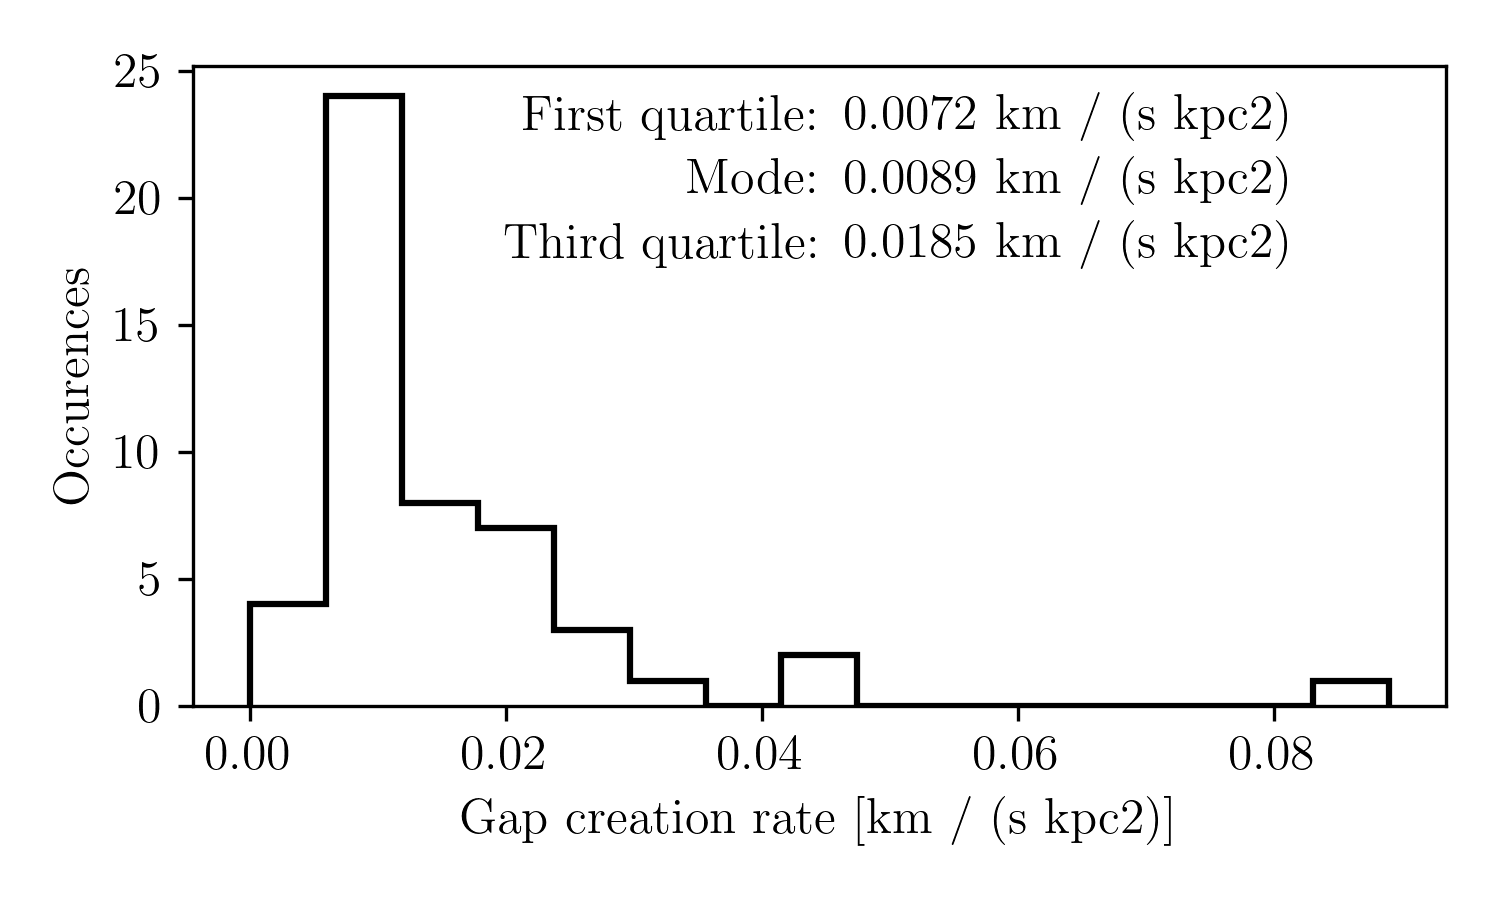
\includegraphics[width=\linewidth]{gap_creation_rate.png}
      \caption{The distribution of the number of gaps normalized over the total integration time and unit stream length, as described by Eq.~\ref{eq:gap_creation_rate} for the whole set of 50 \texttt{full} simulations. }
      \label{fig:gapcreationrate}
    \end{figure}


    Lastly, we note that of the 73 observed gaps\DIFdelbegin \DIFdel{only 8 }\DIFdelend \DIFaddbegin \DIFadd{, only eight }\DIFaddend are in the trailing tail\DIFaddbegin \DIFadd{, }\DIFaddend and the rest are in the leading tail\DIFdelbegin \DIFdel{. This }\DIFdelend \DIFaddbegin \DIFadd{, which }\DIFaddend is a surprising result. A priori, since the \DIFdelbegin \DIFdel{number of star-particles }\DIFdelend \DIFaddbegin \DIFadd{star particles }\DIFaddend escape at similar rates from the \DIFdelbegin \DIFdel{L1 and L2 }\DIFdelend \DIFaddbegin \DIFadd{L$_1$ and L$_2$ }\DIFaddend Lagrange points, each tail is of similar length and density. The main difference between the two tails is that the leading tail is closer to the Galactic center than the trailing tail by about 400~pc. Since the lengths are equal, and the offset between the tails is \DIFdelbegin \DIFdel{small }\DIFdelend \DIFaddbegin \DIFadd{slight }\DIFaddend compared to the galactocentric distance of about 10 kpc, we expected the \DIFdelbegin \DIFdel{number of }\DIFdelend gaps in each tail to be more or less the same. We can compute the probability of observing the unequal occurrences through the binomial distribution. First, \DIFdelbegin \DIFdel{the }\DIFdelend since the 44 gaps linked to NGC~2808 are the same fly-by, they are not independent events. We remove them from this consideration\DIFdelbegin \DIFdel{. This }\DIFdelend \DIFaddbegin \DIFadd{, which }\DIFaddend leaves 21 gaps in the leading tail and 8 in the trailing. The probability of observing up to 8 successes in 29 trials, given a 50\% chance of success, is 1.2\%--unlikely, but possible. Additionally, other perturbers impact at consistent times, which may \DIFdelbegin \DIFdel{also }\DIFdelend violate the assumption of independent events, as seen with NGC~2808.


   
  \subsection{Impact geometry and parameters of the perturbers}\label{sect:geometry}

    \begin{figure*}
      \centering
      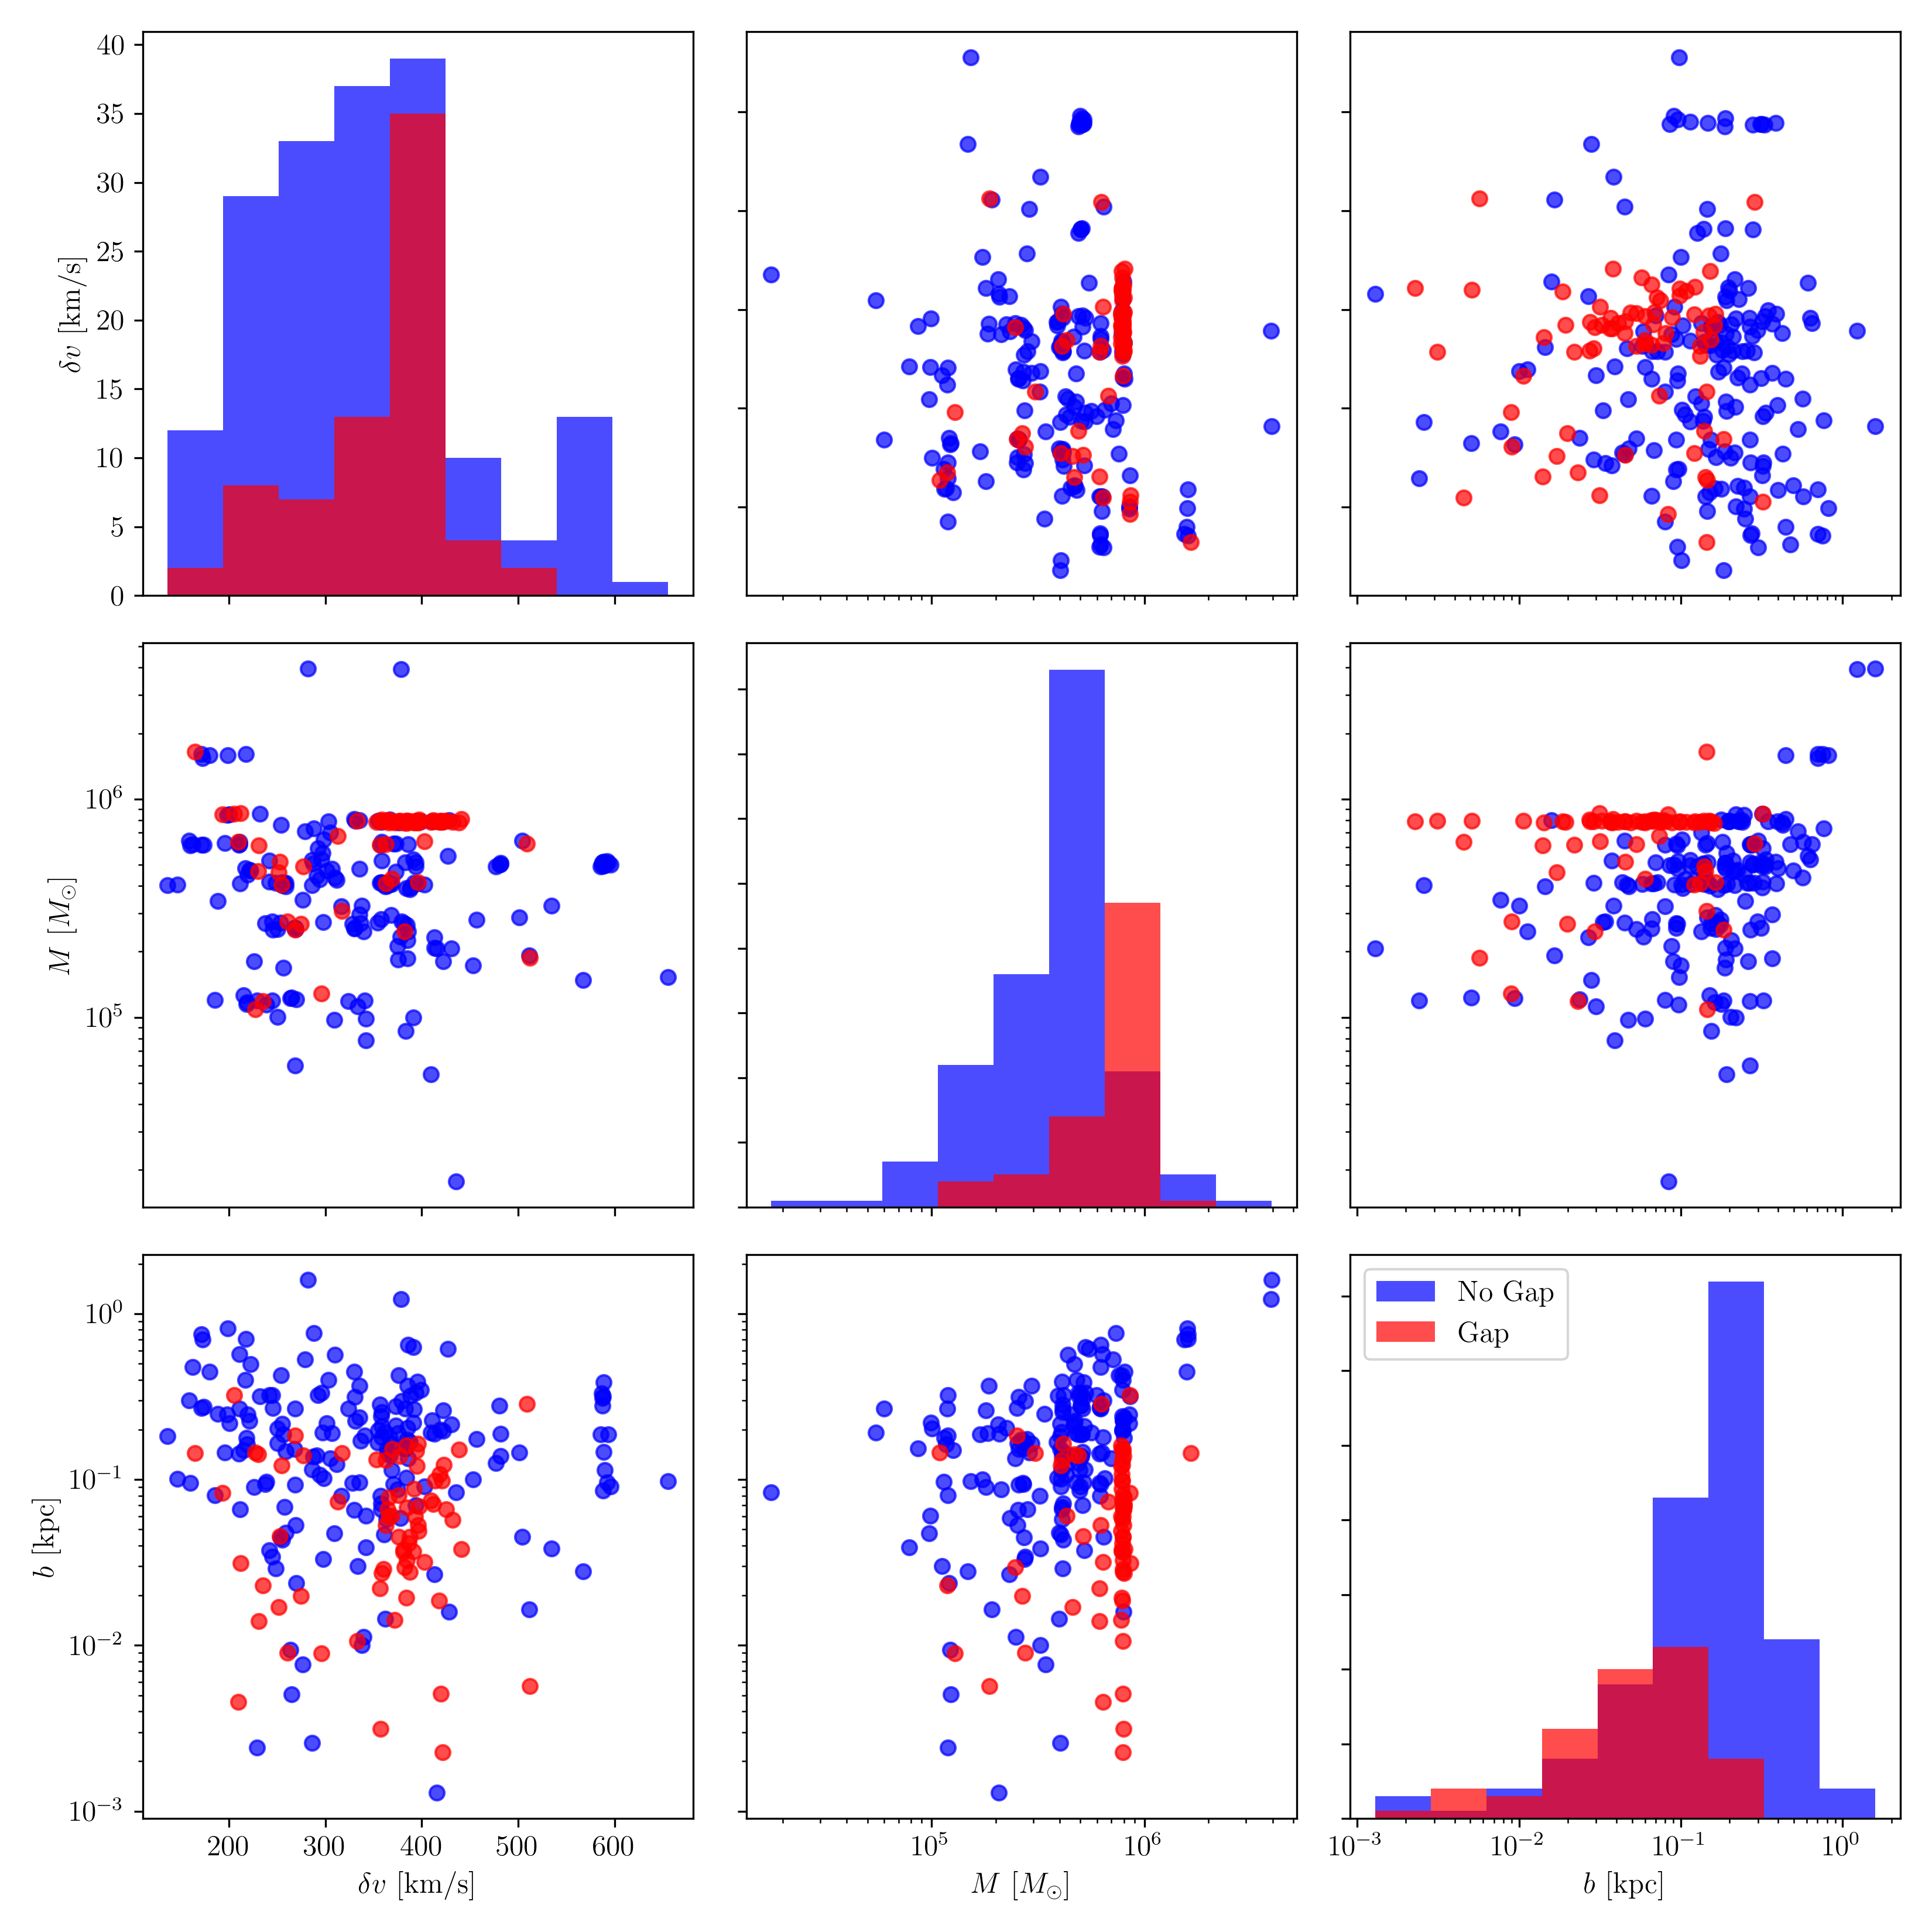
\includegraphics[width=\linewidth]{impact_geometry_statistics.png}
      \caption{The distribution and relationship between the impact variables from Eq.~\ref{eq:change_in_momentum} for all close fly-bys considered. The \DIFaddbeginFL \DIFaddFL{colors indicate the }\DIFaddendFL encounters that cause gaps \DIFaddbeginFL \DIFaddFL{and }\DIFaddendFL are \DIFdelbeginFL \DIFdelFL{labeled with }\DIFdelendFL the same \DIFdelbeginFL \DIFdelFL{colors }\DIFdelendFL as \DIFdelbeginFL \DIFdelFL{from }\DIFdelendFL Fig.~\ref{fig:histogram_impact_time}\DIFdelbeginFL \DIFdelFL{in the scatter plot}\DIFdelendFL , with white \DIFdelbeginFL \DIFdelFL{rings }\DIFdelendFL edges for visibility \DIFdelbeginFL \DIFdelFL{, }\DIFdelendFL and binned in red for the histograms. The \DIFaddbeginFL \DIFaddFL{black histogram shows the }\DIFaddendFL close encounters that did not lead to gaps\DIFdelbeginFL \DIFdelFL{are shown in black}\DIFdelendFL . Indeed, no obvious trend \DIFaddbeginFL \DIFaddFL{has emerged }\DIFaddendFL delimiting these planes into \DIFdelbeginFL \DIFdelFL{gap producing }\DIFdelendFL \DIFaddbeginFL \DIFaddFL{gap-producing }\DIFaddendFL or not\DIFdelbeginFL \DIFdelFL{emerges}\DIFdelendFL .}
      \label{fig:impact_geometry_statistics}    
    \end{figure*}



    With the perturbers identified, we perform statistics \DIFdelbegin \DIFdel{in the pursuit of understanding }\DIFdelend \DIFaddbegin \DIFadd{to understand }\DIFaddend what conditions are necessary for a globular cluster to induce a gap on the Palomar~5 stream. We turn to impact theory, which in its simplest form is presented in works such as \citet{2008gady.book.....B}. Consider two particles: one stationary and the other moving past it. The \DIFaddbegin \DIFadd{impact parameter is the }\DIFaddend distance between the two particles at their closest approach\DIFdelbegin \DIFdel{is known as the impact parameter. To simplify the analysis, the }\DIFdelend \DIFaddbegin \DIFadd{. The }\DIFaddend \textit{impulse approximation} is employed, which assumes that the velocity of the perturber remains unchanged during the interaction. This assumption simplifies the computation.

    To understand how the impacted particle is perturbed, one needs to compute its change in momentum, which is determined by integrating the force acting on the particle \DIFdelbegin \DIFdel{over the duration of the }\DIFdelend \DIFaddbegin \DIFadd{throughout the }\DIFaddend interaction. A useful approximation for this change in momentum, per unit mass, is the force at the closest approach multiplied by an estimate of the interaction time:
    \begin{equation} \label{eq:change_in_momentum} \Delta p \approx \text{Force} \times \text{interaction time} = \frac{GM}{b^2} \times 2\frac{b}{\delta v} = 2\frac{GM}{b \delta v}, \end{equation}where $M$ is the mass of the perturber, $b$ is the impact parameter, $\delta v$ is the relative velocity of the perturber with respect to the particle, and $G$ is the gravitational constant. 


    This equation asserts that a more massive perturber, passing closer to the particle \DIFdelbegin \DIFdel{, }\DIFdelend and moving more slowly, will have a greater impact. It is important to note that the momentum change is inversely proportional to the velocity of the perturber. Note that this contrasts with the intuition from elastic collisions\DIFaddbegin \DIFadd{, }\DIFaddend such as those between billiard balls\DIFaddbegin \DIFadd{, }\DIFaddend where higher velocities result in greater impacts.

    \citet{2015MNRAS.450.1136E} extended this impact theory from one point mass impacting another to studying how an extended body impacts a stream \DIFdelbegin \DIFdel{. This quantifies }\DIFdelend \DIFaddbegin \DIFadd{by quantifying }\DIFaddend the change in momentum of a given particle as a function of its distance from the point of greatest impact along the stream. \DIFdelbegin \DIFdel{In their analysis, the perturber was modeled }\DIFdelend \DIFaddbegin \DIFadd{\mbox{%DIFAUXCMD
\citet{2015MNRAS.450.1136E} }\hskip0pt%DIFAUXCMD
models their perturber }\DIFaddend as a Plummer sphere, like in our simulations. Since the stream \DIFdelbegin \DIFdel{is not zero-dimensional and }\DIFdelend has length, \DIFdelbegin \DIFdel{both }\DIFdelend \DIFaddbegin \DIFadd{one needs to consider }\DIFaddend the parallel and perpendicular components of the \DIFdelbegin \DIFdel{perturber velocity must be considered}\DIFdelend \DIFaddbegin \DIFadd{velocity to describe the impact fully}\DIFaddend . Consequently, five parameters determine the change in velocity of a given stream particle: $M$, $r_p$, $b$, $W_\parallel$, and $W_\perp$, which are the \DIFdelbegin \DIFdel{: }\DIFdelend mass of the perturber, size of the perturber, impact parameter, parallel and perpendicular components of the relative velocity. As detailed in Appendix~\ref{sec:reconstruction}, we calculated these parameters for all our \texttt{full} simulations \DIFdelbegin \DIFdel{, }\DIFdelend by selecting -- for each of them --  the strongest \DIFdelbegin \DIFdel{5 }\DIFdelend \DIFaddbegin \DIFadd{five }\DIFaddend flybys of a perturber with the Palomar~5 stream. Thus, we compute \DIFdelbegin \DIFdel{a total of  }\DIFdelend 250 impacts \DIFdelbegin \DIFdel{, }\DIFdelend and flag those that give way to gaps. 


    Visual inspection of the five key impact parameters ($M$, $r_p$, $b$, $W_\parallel$, and $W_\perp$) did not reveal a clear distinction between flybys that create gaps and those that do not. Therefore, we only present the quantities from Eq.~\ref{eq:change_in_momentum} in Fig.~\ref{fig:impact_geometry_statistics}. 
    Note that \DIFdelbegin \DIFdel{in this figure , we show }\DIFdelend \DIFaddbegin \DIFadd{this figure shows }\DIFaddend the total relative velocity rather than separating parallel and perpendicular components \DIFdelbegin \DIFdel{, because}\DIFdelend \DIFaddbegin \DIFadd{because, }\DIFaddend from a visual inspection, we could not find any specific trends when \DIFaddbegin \DIFadd{we plotted }\DIFaddend the two velocity components \DIFdelbegin \DIFdel{were plotted }\DIFdelend separately. We also \DIFdelbegin \DIFdel{exclude }\DIFdelend \DIFaddbegin \DIFadd{excluded }\DIFaddend the characteristic cluster radius, \DIFdelbegin \DIFdel{as it }\DIFdelend \DIFaddbegin \DIFadd{which }\DIFaddend showed little correlation with the results, likely due to the narrow range of globular cluster radii (see Fig.~\ref{fig:mass_size_plane}). This factor might be more significant for dark matter sub-halos, where size variation is greater.

      
  
    While Fig.~\ref{fig:impact_geometry_statistics} demonstrates that mass, relative velocity, or impact parameter alone cannot predict gap formation, one interesting result emerges: \DIFdelbegin \DIFdel{no gaps are created from interactions with }\DIFdelend impact parameters greater than 300~pc \DIFaddbegin \DIFadd{do not create gaps}\DIFaddend . The stream widths are roughly 200~pc, as seen in Appendix~\ref{sec:gallery_of_gaps}. This finding is even more evident when examining the $b$-$M$ plane. A series of perturbers at roughly $\sim8 \times 10^5 M_\odot$ highlights NGC~2808's flybys, where all encounters with impact parameters under 200~pc result in gaps, while those beyond this distance do not. In other words, even the most massive \DIFdelbegin \DIFdel{globulars }\DIFdelend \DIFaddbegin \DIFadd{globular clusters }\DIFaddend with masses greater than about $10^6 M_\odot$ cannot cause gaps if their impact parameters are greater than \DIFdelbegin \DIFdel{about }\DIFdelend \DIFaddbegin \DIFadd{roughly }\DIFaddend $300$~pc. \DIFdelbegin \DIFdel{It is interesting to note that for values of the impact parameter below this threshold}\DIFdelend \DIFaddbegin \DIFadd{Interestingly}\DIFaddend , even fast encounters ($\delta v > 300$~km/s) can produce gaps \DIFdelbegin \DIFdel{. Perhaps, }\DIFdelend \DIFaddbegin \DIFadd{for impact parameter values below this threshold. Perhaps }\DIFaddend this is not surprising since the range of possible relative velocities is much less than mass and impact \DIFdelbegin \DIFdel{parameter which vary }\DIFdelend \DIFaddbegin \DIFadd{parameters, which vary by }\DIFaddend two and three orders \DIFdelbegin \DIFdel{, respectively while }\DIFdelend \DIFaddbegin \DIFadd{of magnitude, respectively. In contrast, }\DIFaddend the relative velocities only vary by about a factor of three.

    \begin{figure}
      \centering
      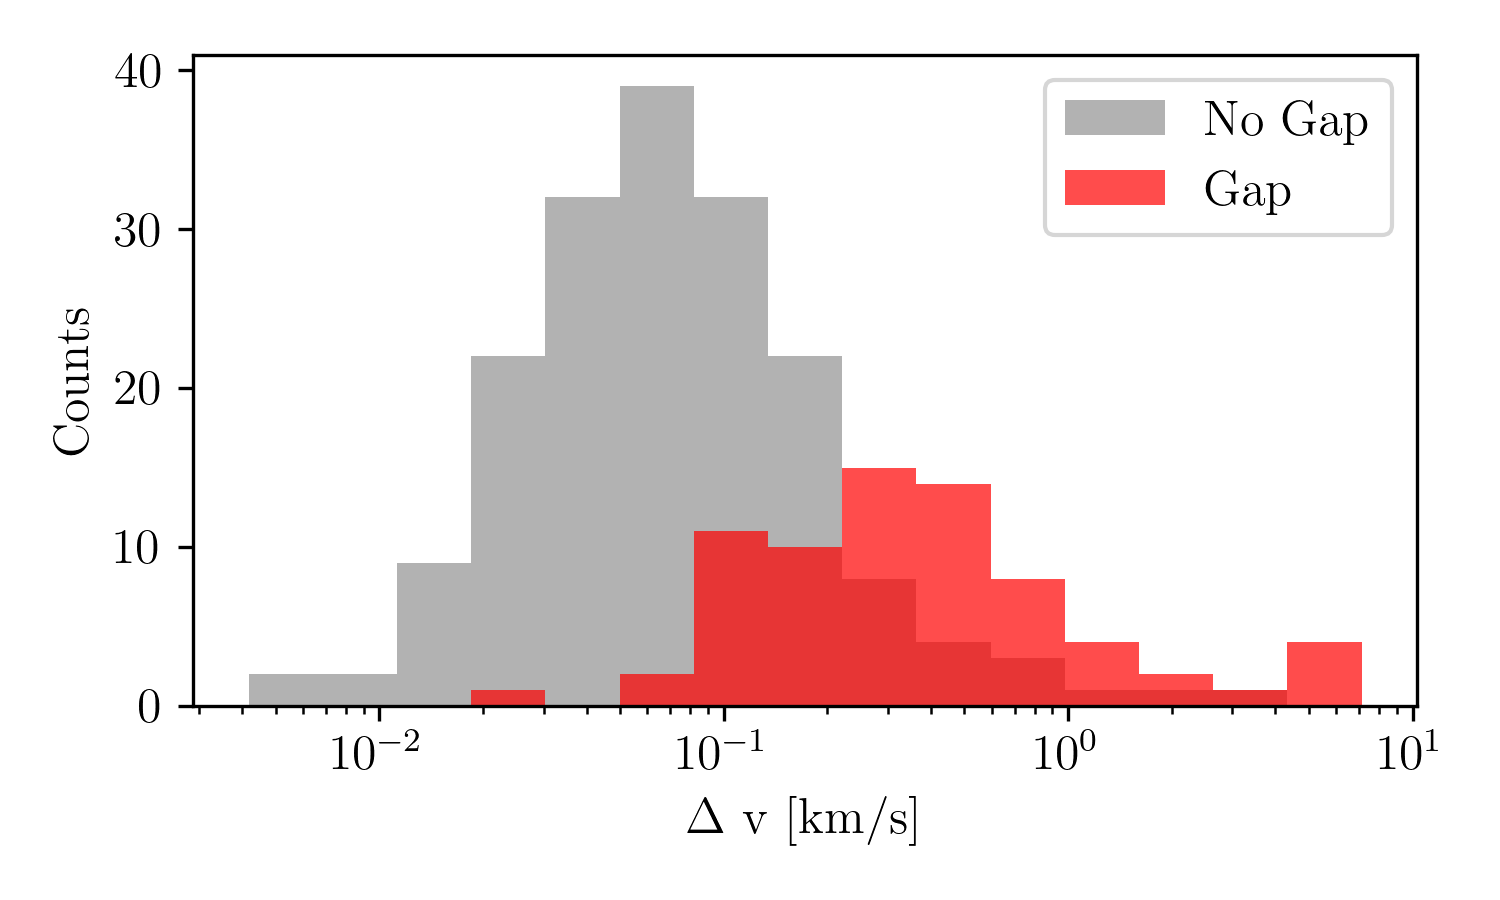
\includegraphics[width=1\linewidth]{impact_geometry_statistics_deltaP.png}
      \caption{The distribution of imparted change in momentum (per unit mass) from a cluster flyby given by Eq.~\ref{eq:change_in_momentum}. The data set includes the top 5 strongest flybys from each simulation. Those that cause gaps are colored, stacked, and overlain atop \DIFdelbeginFL \DIFdelFL{of }\DIFdelendFL those that \DIFdelbeginFL \DIFdelFL{do--the distribution of which }\DIFdelendFL \DIFaddbeginFL \DIFaddFL{do not--which }\DIFaddendFL is \DIFdelbeginFL \DIFdelFL{outlined in grey}\DIFdelendFL \DIFaddbeginFL \DIFaddFL{the gray distribution}\DIFaddendFL . Note that the meaning of the colors is the same as in Fig.~\ref{fig:histogram_impact_time}.}
      \label{fig:deltap}
    \end{figure}

    \begin{figure*}
      \centering
      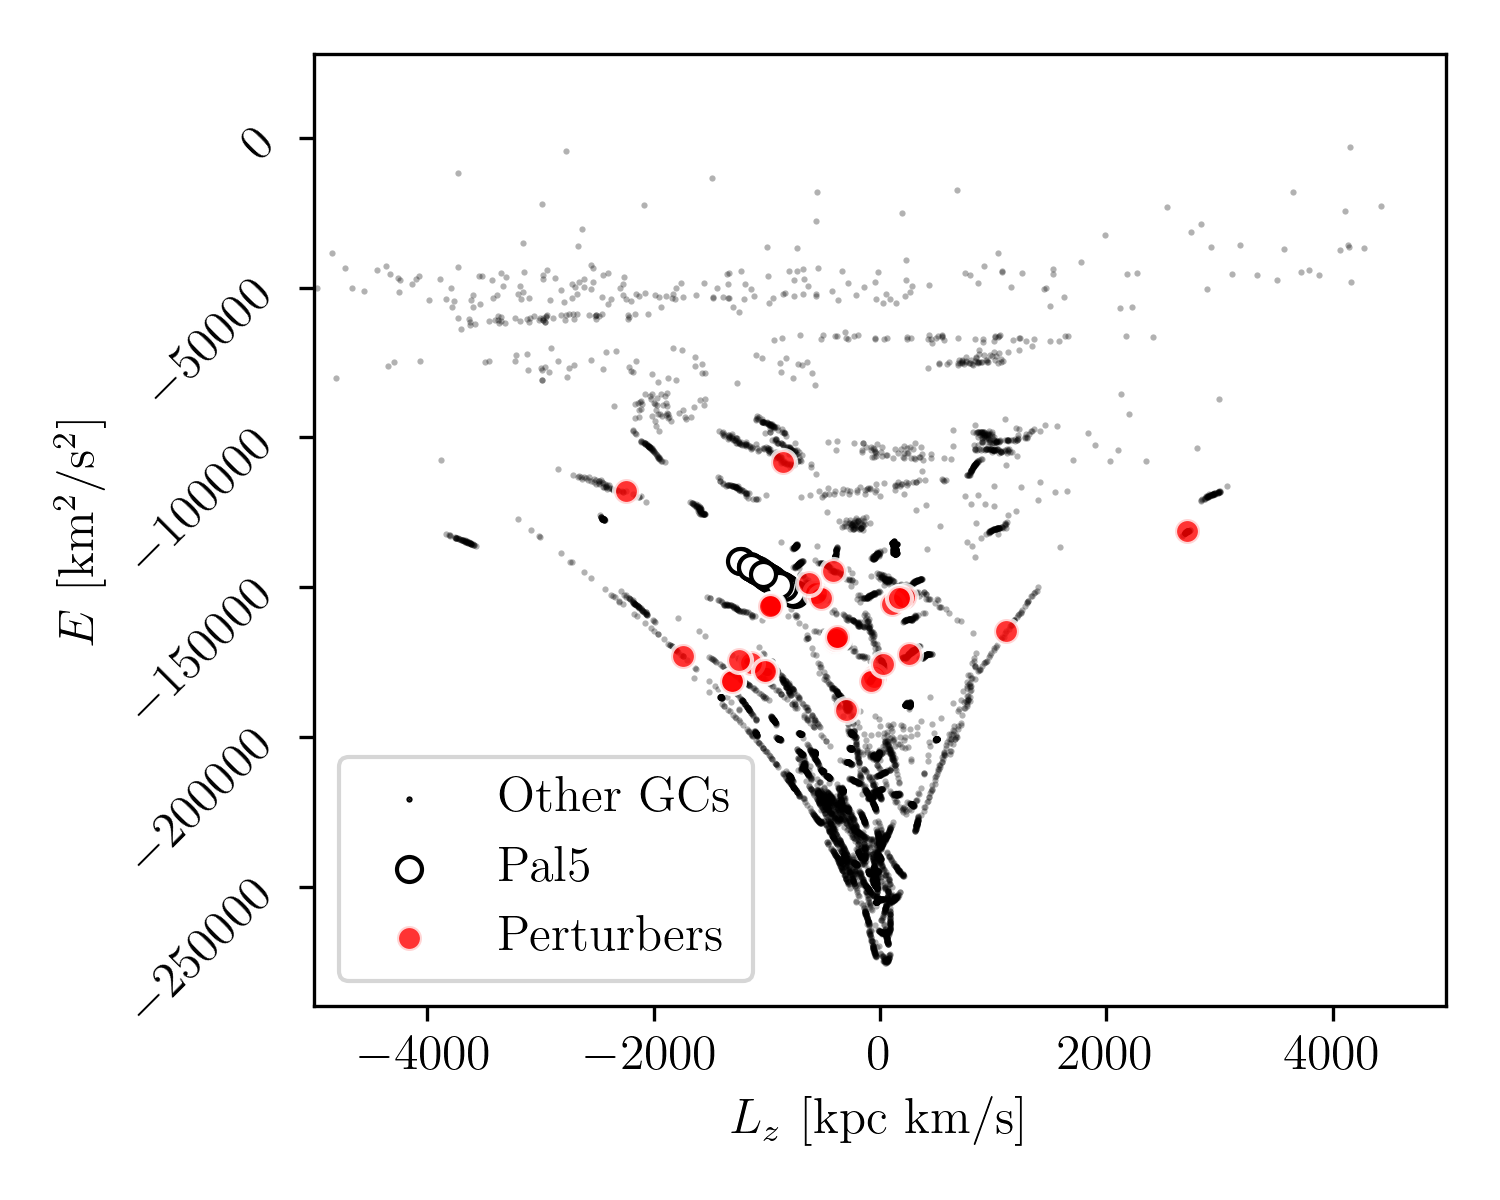
\includegraphics[width=0.45\linewidth]{E_Lz_perturbers.png}
      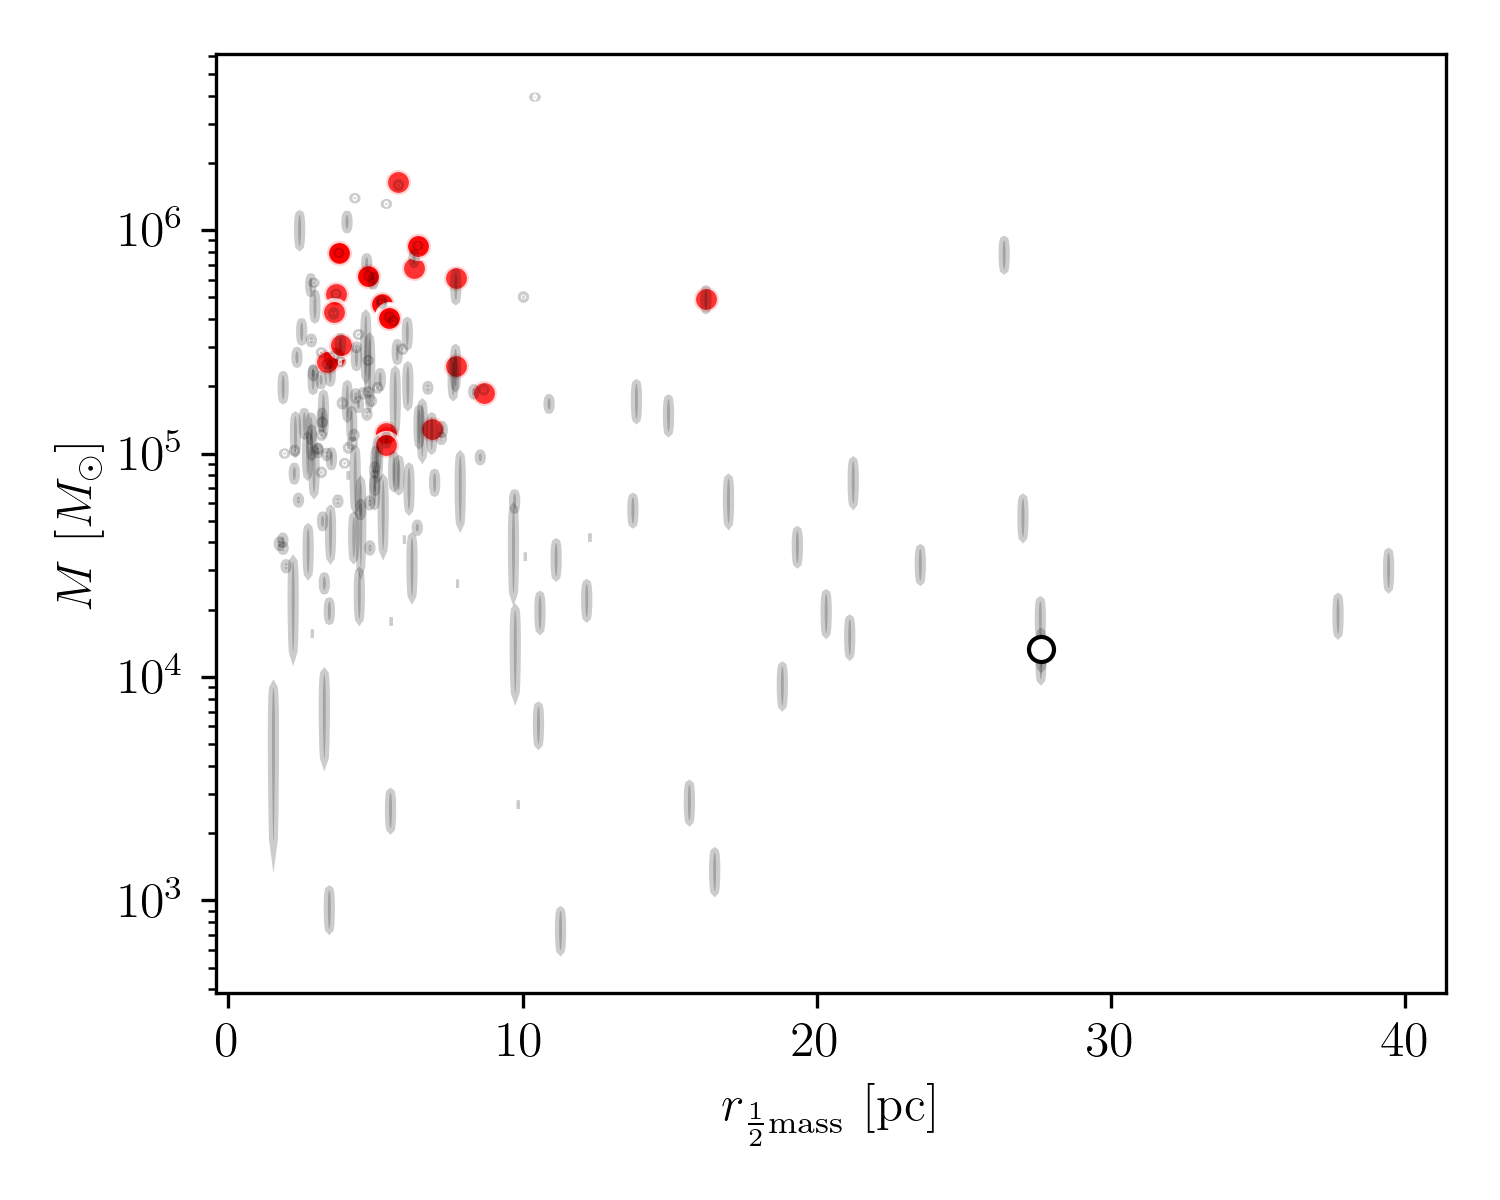
\includegraphics[width=0.45\linewidth]{mass_size_plane.png}
      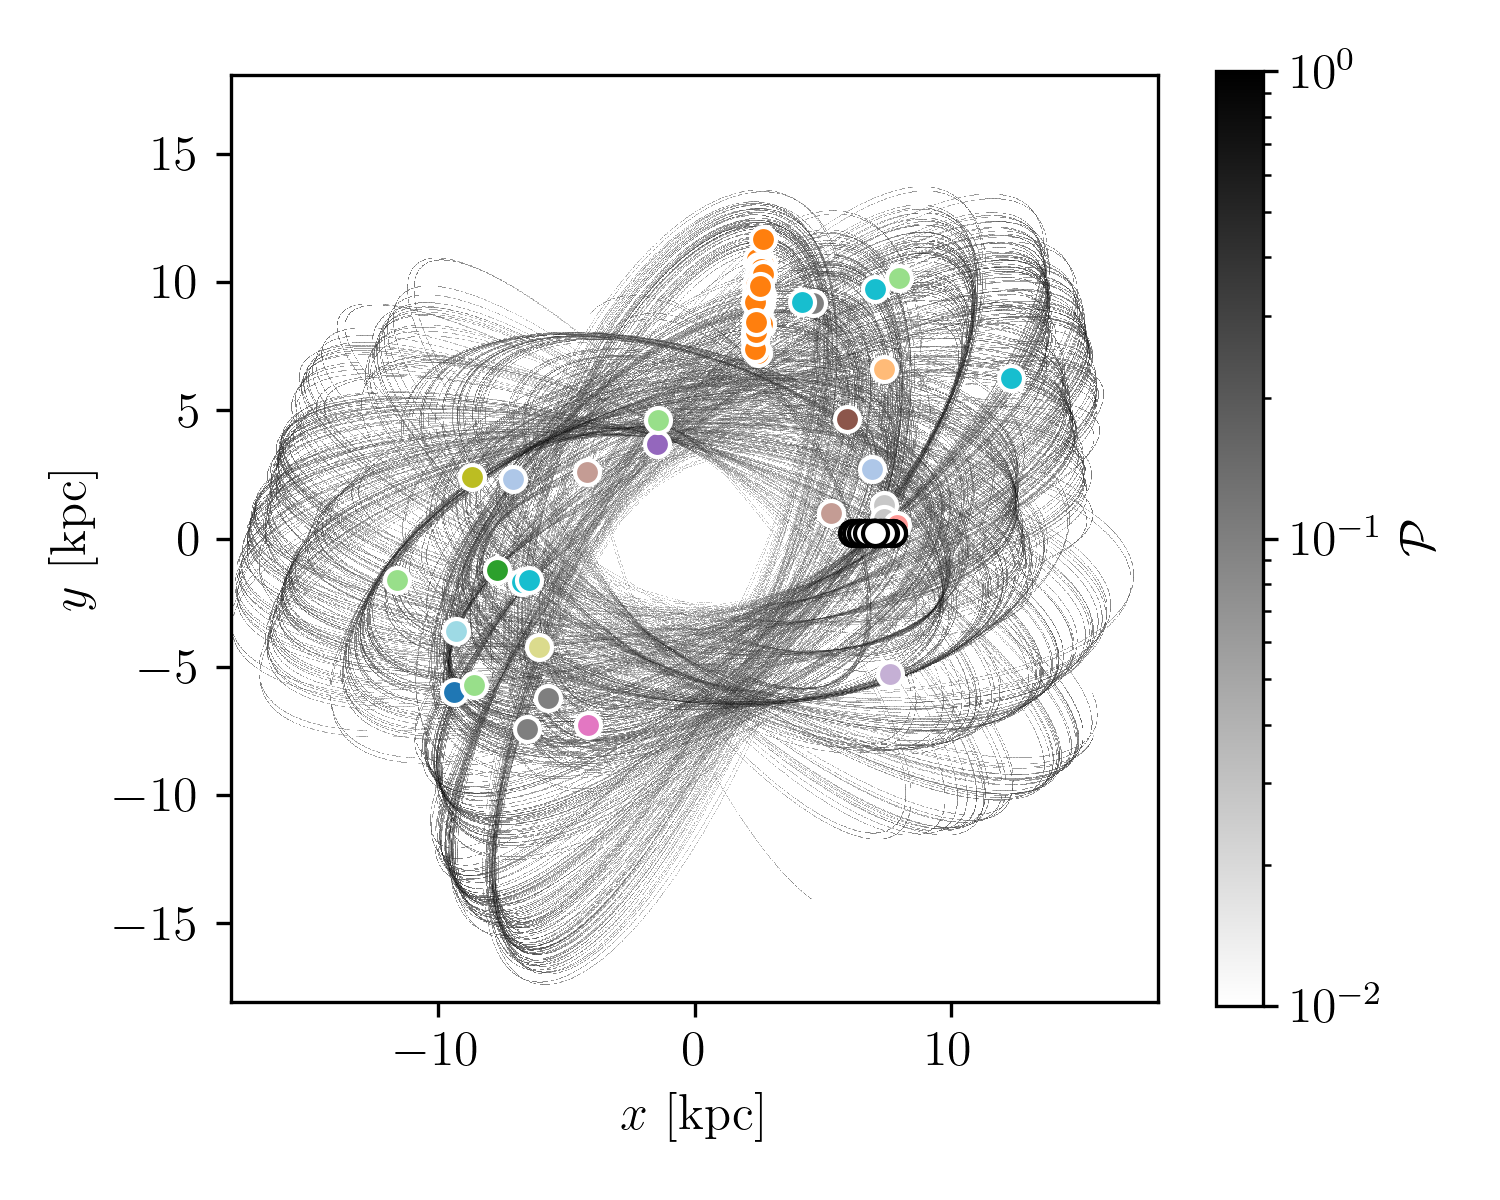
\includegraphics[width=0.45\linewidth]{impact_stats_phase_space_xy.png}
      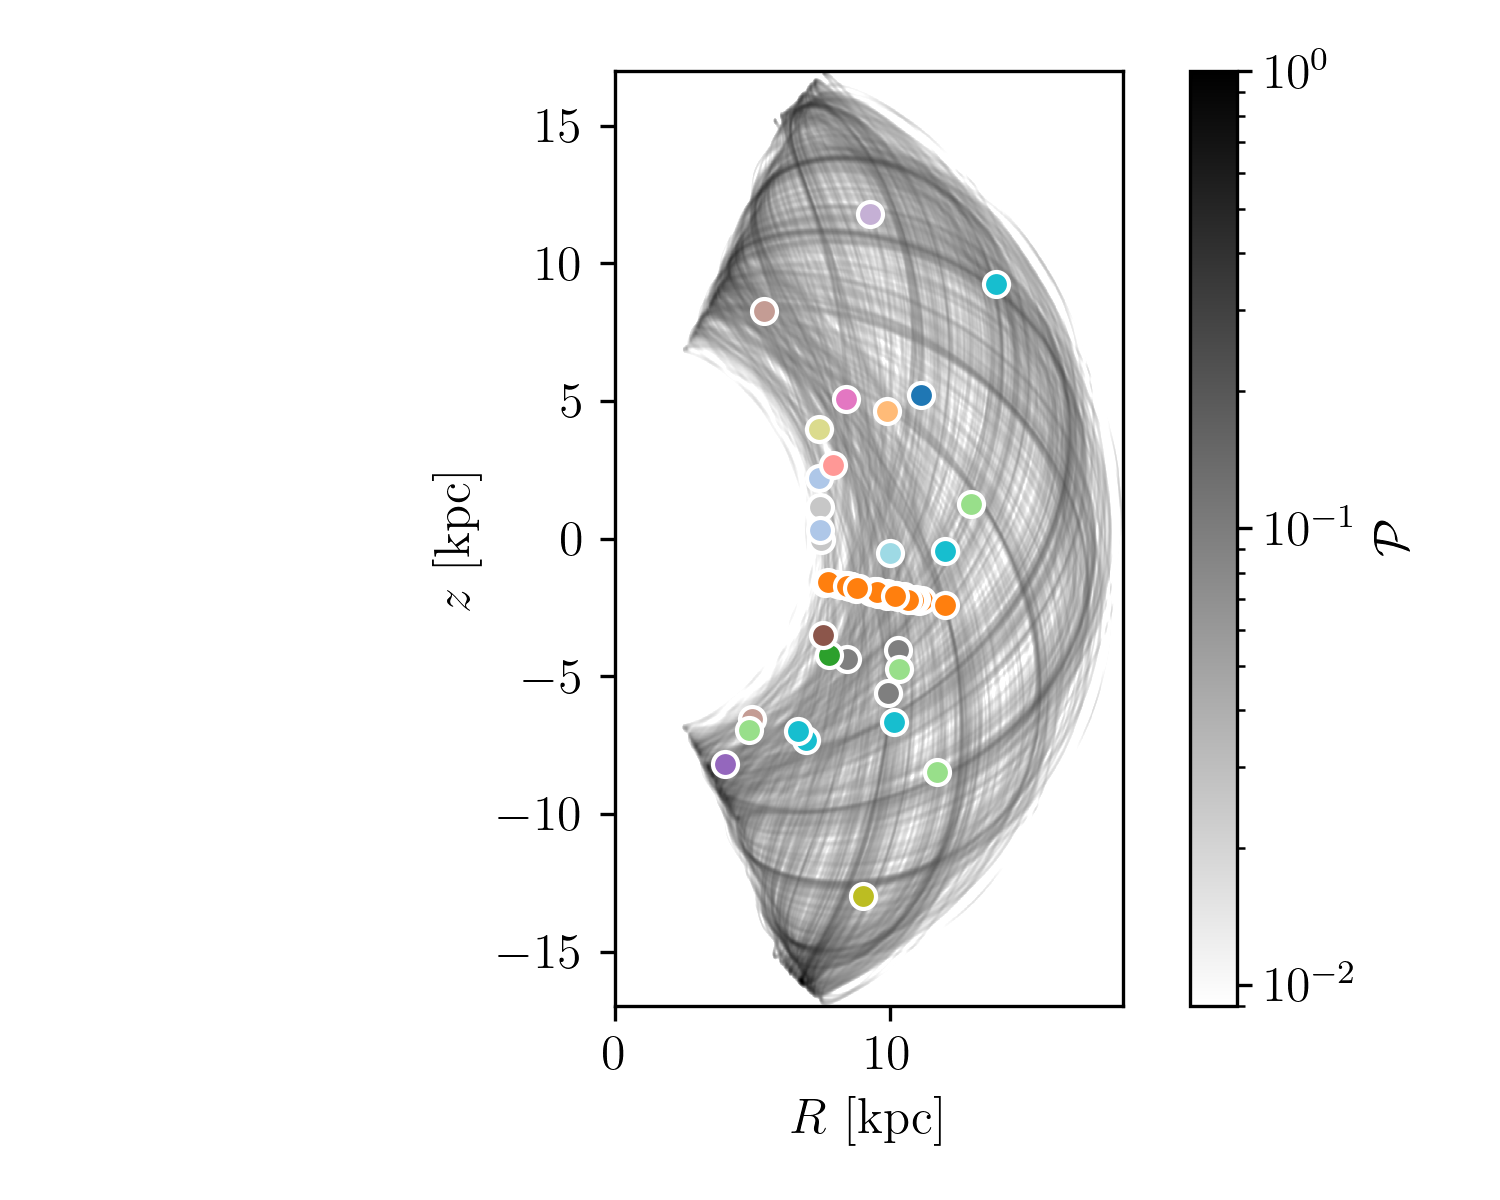
\includegraphics[width=0.45\linewidth]{impact_stats_phase_space.png}
      \caption{\textit{Characteristics of gap causing clusters}. \textit{Top Left:} Energy-angular momentum space of the globular clusters in the simulations, with 50~$\times$~165 data points representing all sampled initial conditions. Clusters impacting Palomar~5 are shown with colored markers\DIFdelbeginFL \DIFdelFL{; }\DIFdelendFL \DIFaddbeginFL \DIFaddFL{, }\DIFaddendFL large for the samplings that induce a gap and small for those that do not. \DIFdelbeginFL \DIFdelFL{Non-gap-causing clusters are shown in }\DIFdelendFL \DIFaddbeginFL \DIFaddFL{The }\DIFaddendFL small gray dots \DIFaddbeginFL \DIFaddFL{represent the non-gap-causing clusters}\DIFaddendFL . The 50 white dots indicate Palomar~5's sampled initial conditions for the current day position. The \DIFdelbeginFL \DIFdelFL{circular velocity-curve is drawn with a }\DIFdelendFL light-pink dashed curve \DIFaddbeginFL \DIFaddFL{shows the circular velocity curve}\DIFaddendFL . \textit{Top Right:} Mass-size plane of the globular clusters in the simulations, with uncertainties on the masses indicated as vertical lines. We remind the reader that the globular cluster catalog \DIFdelbeginFL \DIFdelFL{at this time }\DIFdelendFL \DIFaddbeginFL \DIFaddFL{currently }\DIFaddendFL does not provide uncertainties for clusters' characteristic radii. \textit{Bottom Left:} Palomar~5's orbit in the Galactocentric xy plane. The \DIFdelbeginFL \DIFdelFL{gray-scale }\DIFdelendFL \DIFaddbeginFL \DIFaddFL{gray scale }\DIFaddendFL represents all 50 stacked orbits, with $\mathcal{P}$ indicating the probability of Palomar~5's position, normalized to $\mathcal{P}_\textrm{max}=1$. The colored markers indicate \DIFdelbeginFL \DIFdelFL{where }\DIFdelendFL the \DIFaddbeginFL \DIFaddFL{position of the }\DIFaddendFL perturber \DIFdelbeginFL \DIFdelFL{was located }\DIFdelendFL when it impacted the stream and \textit{not} its \DIFdelbeginFL \DIFdelFL{present day }\DIFdelendFL \DIFaddbeginFL \DIFaddFL{present-day }\DIFaddendFL position. \textit{Bottom Right:} same as \DIFaddbeginFL \DIFaddFL{the }\DIFaddendFL bottom left but in the meridional plane. In all panels\DIFaddbeginFL \DIFaddFL{, }\DIFaddendFL the colors of the markers and histogram bars correspond to specific \DIFdelbeginFL \DIFdelFL{perturber }\DIFdelendFL \DIFaddbeginFL \DIFaddFL{perturbers }\DIFaddendFL as specified in Fig.~\ref{fig:histogram_impact_time}.}
      \label{fig:mass_size_plane}
    \end{figure*}

      
    Once all the key impact parameters \DIFaddbegin \DIFadd{are }\DIFaddend estimated, we can use Eq.~\ref{eq:change_in_momentum} and calculate $\Delta p$, the change in momentum (per unit mass) imparted by a cluster flyby on Palomar~5 stream. \DIFdelbegin \DIFdel{The result  is shown in }\DIFdelend Fig.~\ref{fig:deltap} \DIFdelbegin \DIFdel{, where }\DIFdelend \DIFaddbegin \DIFadd{shows }\DIFaddend the distribution of imparted change in momentum \DIFdelbegin \DIFdel{is shown }\DIFdelend for all impacts \DIFdelbegin \DIFdel{which }\DIFdelend \DIFaddbegin \DIFadd{that }\DIFaddend produce a gap \DIFdelbegin \DIFdel{, and }\DIFdelend compared to those that do not\DIFdelbegin \DIFdel{produce one}\DIFdelend . On average, encounters \DIFdelbegin \DIFdel{which }\DIFdelend \DIFaddbegin \DIFadd{that }\DIFaddend lead to gap \DIFdelbegin \DIFdel{creations }\DIFdelend \DIFaddbegin \DIFadd{creation }\DIFaddend impart a change in momentum on stream particles\DIFaddbegin \DIFadd{, }\DIFaddend which is a factor of 10 higher than \DIFdelbegin \DIFdel{that of encounters which }\DIFdelend \DIFaddbegin \DIFadd{encounters that }\DIFaddend do not form gaps (but with some overlap in the low-velocity tail). Interestingly, changes in momentum\DIFaddbegin \DIFadd{, }\DIFaddend which lead to gap creations\DIFaddbegin \DIFadd{, }\DIFaddend extend over a large range in velocities. There is a factor of about 100 between the smallest and largest changes with NGC~2808 (orange color in the histogram) imparting changes in the velocity of stream particles\DIFaddbegin \DIFadd{, }\DIFaddend which redistribute over the whole range of $\Delta p$. 

    In addition to characterizing the parameters governing cluster encounters with the stream, since we know which clusters have produced gaps on the tail of Palomar~5, we can also verify their orbital and structural properties. \DIFdelbegin \DIFdel{This is shown in }\DIFdelend Fig~\ref{fig:mass_size_plane} \DIFaddbegin \DIFadd{shows just this}\DIFaddend , where we first show the \DIFaddbegin \DIFadd{clusters' }\DIFaddend mass and size (i.e.\DIFaddbegin \DIFadd{, }\DIFaddend half-mass radius) \DIFdelbegin \DIFdel{of the clusters }\DIFdelend that cause gaps on the tails of Palomar~5, dividing them from those that do not. As can be seen, no cluster with mass below $10^5 M_\odot$ causes gaps on the Palomar~5 stream, and all perturbers, except FSR~1758\DIFaddbegin \DIFadd{, }\DIFaddend have a half-mass radius below 10~pc. Even more interesting is their distribution in the E-L$_z$ plane, which shows that the clusters that cause gaps are on both direct and retrograde orbits (\DIFdelbegin \DIFdel{respectively, }\DIFdelend negative and positive values of $L_z$)\DIFdelbegin \DIFdel{, but all confined to }\DIFdelend \DIFaddbegin \DIFadd{. However, all of the perturbers exist in }\DIFaddend an energy interval between $-2$ and $-1 \times10^5~\textrm{km}^2\textrm{s}^{-2}$\DIFdelbegin \DIFdel{. This }\DIFdelend \DIFaddbegin \DIFadd{, which }\DIFaddend is because only clusters within Palomar~5's orbital space can interact with the stream: clusters with higher orbital energies tend to have larger \DIFdelbegin \DIFdel{apocenter }\DIFdelend \DIFaddbegin \DIFadd{apocenters }\DIFaddend than that of Palomar~5 and thus spend most of their time away from Palomar~5's orbital volume. 

    Finally, it is worth commenting on the location of impacts with the stream, whether they occur when Palomar~5 is close to its pericenter\DIFdelbegin \DIFdel{or not. As it can be seen from }\DIFdelend \DIFaddbegin \DIFadd{. }\DIFaddend Fig.~\ref{fig:mass_size_plane}\DIFdelbegin \DIFdel{(bottom panel ) }\DIFdelend \DIFaddbegin \DIFadd{'s bottom panel shows that }\DIFaddend encounters can occur at all orbital phases of Palomar~5, when it is close to \DIFaddbegin \DIFadd{the }\DIFaddend pericenter, but also very far away from it, at the outskirts of its orbital space. However, when taken all together, the location of \DIFdelbegin \DIFdel{gap creating }\DIFdelend \DIFaddbegin \DIFadd{gap-creating }\DIFaddend impacts shows a strong negative correlation with the galactocentric radius $r$, with the number $N$ of encounters favorable to gap formation going as $N = -2.5r + 50$ (with a Pearson coefficient of -0.86). While there are more clusters near the Galactic center, clusters naturally spend more time near their apocenters, and the lower relative velocities in these regions should favor gap creation. However, this result suggests that \DIFaddbegin \DIFadd{the }\DIFaddend cluster Galactic number density outweighs these factors \DIFdelbegin \DIFdel{in }\DIFdelend \DIFaddbegin \DIFadd{when }\DIFaddend determining the number of gaps. \DIFdelbegin \DIFdel{It should be noted that these }\DIFdelend \DIFaddbegin \DIFadd{The }\DIFaddend results are for Palomar~5 only\DIFdelbegin \DIFdel{. Streams }\DIFdelend \DIFaddbegin \DIFadd{, and a future study would need to investigate streams }\DIFaddend along various orbits \DIFdelbegin \DIFdel{need to be studied in order for this conclusionto be generalized}\DIFdelend \DIFaddbegin \DIFadd{before generalizing this conclusion}\DIFaddend .


    %DIF < Our results are consistent with the findings from \citet{2021MNRAS.505.5978V}, who identified a wide range of orbital solutions for the least bound clusters, including both retrograde and prograde orbits. In our potential model, only three clusters samplings had positive orbital energies.
%DIF > Our results are consistent with the findings from \citet{2021MNRAS.505.5978V}, who identified a wide range of orbital solutions for the least bound clusters, including retrograde and prograde orbits. In our potential model, only three cluster samplings had positive orbital energies.


  \subsection{Comparison to observations}

    We briefly compare our simulated gaps to the literature on Palomar~5. In the bottom panel of Fig.~\ref{fig:decomposition}, we compare the tracks of Palomar~5 that were compiled in \texttt{galstreams} by \citet{2023MNRAS.520.5225M}. The mid-point positions of the streams do not have the same \DIFdelbegin \DIFdel{galacto-centric }\DIFdelend \DIFaddbegin \DIFadd{galactocentric }\DIFaddend positions as Palomar~5 from Baumgardt's catalog\DIFdelbegin \DIFdel{and are thus }\DIFdelend \DIFaddbegin \DIFadd{, and the difference creates an }\DIFaddend offset when projected into tail coordinates. Moreover, since we sample the distances to Palomar~5, the galactocentric position within the Baumgardt catalog varies. To combat this, we position the mid-point of the \DIFdelbegin \DIFdel{Galstream }\DIFdelend \DIFaddbegin \texttt{\DIFadd{Galstream}} \DIFaddend tracks at the \DIFaddbegin \DIFadd{cluster's }\DIFaddend center of mass\DIFdelbegin \DIFdel{of the cluster, which allows }\DIFdelend \DIFaddbegin \DIFadd{, allowing }\DIFaddend us to compare the length of the observed tracks to our simulated streams. We use the three tracks Pal5-PW19, Pal5-S20, and Pal5-I21 from \citet{2019AJ....158..223P}, \citet{2020MNRAS.495.2222S}, and \citet{2021ApJ...914..123I}, respectively. For each track, we find the distance from the cluster in either direction\DIFdelbegin \DIFdel{and }\DIFdelend \DIFaddbegin \DIFadd{, }\DIFaddend count the number of gaps \DIFdelbegin \DIFdel{that fall }\DIFdelend within this range\DIFdelbegin \DIFdel{. This is presented }\DIFdelend \DIFaddbegin \DIFadd{, and present this }\DIFaddend in Fig.~\ref{fig:GapsWithinSight}. In the maximum limit\DIFaddbegin \DIFadd{, }\DIFaddend many gaps could appear \DIFdelbegin \DIFdel{, }\DIFdelend at a rate of about one per realization. However, \DIFdelbegin \DIFdel{at the shortest reported stream-length }\DIFdelend only a few gaps occur \DIFdelbegin \DIFdel{.
      }\DIFdelend \DIFaddbegin \DIFadd{at the shortest reported stream length. We note, in particular, that the gap generated by the recent perturbation induced on the stream by the passage of NGC~2808 (whose occurrence is very likely according to our models) sits in a portion of the simulated tail which is at the edge of the observed one (see bottom panel in Fig.~2). This element and the fact that this gap is skinny, because it is very recent, probably make its detection difficult. 
      }\DIFaddend \begin{figure}
        \centering
        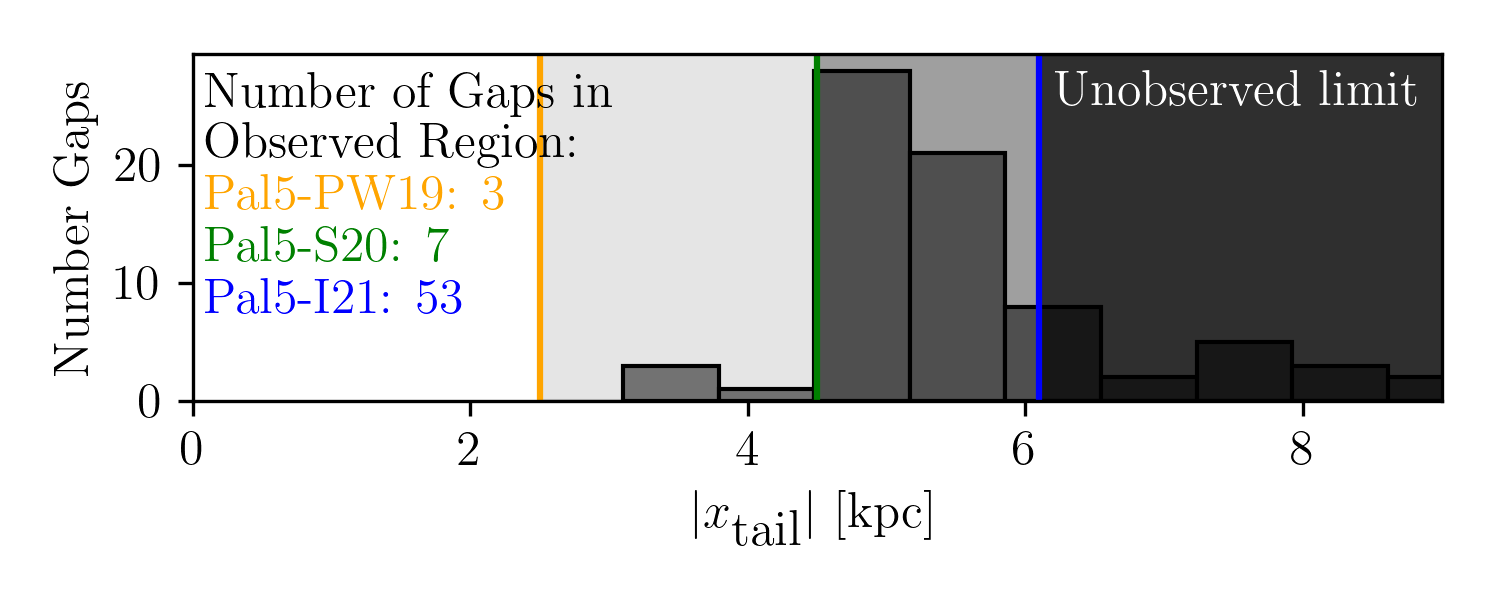
\includegraphics[width=\linewidth]{GapWithinSight.png}
        \caption{The distribution of gaps as a function of absolute distance from the center of mass of Palomar 5's globular cluster. \DIFdelbeginFL \DIFdelFL{The }\DIFdelendFL \DIFaddbeginFL \DIFaddFL{We count the }\DIFaddendFL number of gaps within the observable range \DIFdelbeginFL \DIFdelFL{is evaluated }\DIFdelendFL on an individual track basis, with track lengths determined by the minimum and maximum $x'$-coordinates from the bottom panel of Fig.~\ref{fig:decomposition}. The ranges for \citet{2019AJ....158..223P}, \citet{2020MNRAS.495.2222S}, and \citet{2021ApJ...914..123I} are shown for their respective dimensions, and the number of gaps within these ranges is indicated in the figure. Vertical bars mark the $x' > 0$ limit of the stream--we only show the \DIFdelbeginFL \DIFdelFL{right hand }\DIFdelendFL \DIFaddbeginFL \DIFaddFL{right-hand }\DIFaddendFL side instead of both for clarity, as most gaps are located on the right-hand side of the stream in any case. }
        \label{fig:GapsWithinSight}
      \end{figure}    

    We observe \DIFdelbegin \DIFdel{that there are no gaps near }\DIFdelend \DIFaddbegin \DIFadd{no gaps }\DIFaddend within 3~kpc \DIFdelbegin \DIFdel{to }\DIFdelend \DIFaddbegin \DIFadd{of }\DIFaddend the cluster in our simulation. There may be a few reasons for the absence of gaps in the portion of the tails closer to the cluster center. First, as \citet{2016MNRAS.457.3817S} demonstrated, the dispersion of action-frequencies in the stream plays a role. For instance, the frequency corresponding to the azimuthal action, $J_\phi$, is $\dot\theta_\phi = - \frac{\mathcal{\partial H}}{\partial J_\phi}$ and where $\theta_\phi$ is the angle describing the position of the particle phase space between momentum ($p_\phi$) and position ($\phi$) axes---where $\phi$ is the azimuthal angle between the x-y axes in physical space. \DIFdelbegin \DIFdel{Regions of the stream }\DIFdelend \DIFaddbegin \DIFadd{Stream regions }\DIFaddend with well-separated frequencies are more susceptible to gap formation, while those with a wide frequency range (near the cluster) tend to erase the history of impacts. Thus, for a gap to form, the imparted change in frequency must exceed the range of frequencies in the impacted region. \DIFdelbegin \DIFdel{Thus}\DIFdelend \DIFaddbegin \DIFadd{Therefore}\DIFaddend , the strong flybys \DIFdelbegin \DIFdel{that occurred }\DIFdelend close to the cluster were inconsequential for gap formation. 

    Another possible explanation is the different \DIFdelbegin \DIFdel{thickness }\DIFdelend \DIFaddbegin \DIFadd{thicknesses }\DIFaddend of the simulated tails at different distances from the \DIFdelbegin \DIFdel{center of the cluster}\DIFdelend \DIFaddbegin \DIFadd{cluster's center}\DIFaddend . At distances \DIFdelbegin \DIFdel{of less than about }\DIFdelend \DIFaddbegin \DIFadd{less than }\DIFaddend 3~kpc from Palomar~5, the tails are \DIFdelbegin \DIFdel{very thin}\DIFdelend \DIFaddbegin \DIFadd{skinny}\DIFaddend , with a typical thickness \DIFdelbegin \DIFdel{being }\DIFdelend \DIFaddbegin \DIFadd{of }\DIFaddend less than 100~pc. \DIFdelbegin \DIFdel{In order to }\DIFdelend \DIFaddbegin \DIFadd{To }\DIFaddend cause gaps in these regions, the clusters would have to pass close to the stream, with impact parameters similar to the thickness itself. Note that the thinness of the tails at these distances is probably a direct consequence of the initial parameters we chose for the simulation. \DIFdelbegin \DIFdel{We have assumed for }\DIFdelend \DIFaddbegin \DIFadd{For }\DIFaddend Palomar~5, 5~Gyr years ago, \DIFaddbegin \DIFadd{we assumed }\DIFaddend the same internal parameters (mass and size) \DIFdelbegin \DIFdel{that the cluster has }\DIFdelend \DIFaddbegin \DIFadd{as the cluster }\DIFaddend today. With such parameters, after 5~Gyr of evolution, our system has lost most of its mass, and therefore\DIFaddbegin \DIFadd{, }\DIFaddend the part of the tails closest to the cluster itself, whose density depends mainly on the most recent mass loss \citep[see, for example, Fig.~A.3 in][]{2012A&A...546L...7M}, is necessarily very thin because the simulated cluster has essentially no more mass to lose. This last point \DIFdelbegin \DIFdel{has also }\DIFdelend \DIFaddbegin \DIFadd{also has }\DIFaddend a consequence in the gap creation rate, which we derived at the end of Sect.~\ref{sect:geometry}: with only 70\% of the tail  ($\sim$ 14~kpc over 20~kpc, excluding the innermost $\pm 3$~kpc from the cluster center) \DIFdelbegin \DIFdel{really }\DIFdelend suitable for forming gaps, the gap creation rates are about 50$\%$ higher than those estimated in the \DIFdelbegin \DIFdel{aforementioned }\DIFdelend \DIFaddbegin \DIFadd{previous }\DIFaddend section, where values have been derived taking into account the full tail extent. This gap creation rate would \DIFdelbegin \DIFdel{be still not }\DIFdelend \DIFaddbegin \DIFadd{still not be }\DIFaddend high enough to reproduce the number of gaps in Palomar~5's tails, as reported by \citet{2012ApJ...760...75C}. \DIFdelbegin \DIFdel{In their study , they indeed }\DIFdelend \DIFaddbegin \DIFadd{Their study }\DIFaddend suggested the presence of five gaps with a 99~\% detection confidence, leading to a gap creation rate of 0.17~Gyr$^{-1}$~kpc$^{-1}$. If correct, this rate would be too high to be explained by Galactic globular clusters only. 

\DIFaddbegin \DIFadd{An additional explanation for the absence of gaps in the inner regions of a stream is given in App.~\ref{sec:gaps_vs_gcmass}. Briefly, the eccentricity of an orbit induces tidal shocking at the pericenter passages that cause episodes of increased mass loss where the escaped stars leave with a higher mean velocity and greater velocity dispersion. In essence, streams from progenitors on eccentric orbits are made of two components: a continuous flow of stars plus many packets of stars that burst out from pericenter passages. The gap impact occurs at a single position, creating a gap in each subpopulation. However, the gaps have different drift rates across the groups, and they eventually go out of phase, erasing the impact's signature. The packets of stars disperse with time. However, bursts contribute to more escaped stars as the simulation evolves than the continuous outflow. As a result, at late stages of the simulation, the region nearest to the globular cluster is made of distinct yet overlapping populations. After an impact in this location, the impact site between the groups quickly goes out of phase. 
}

  
  
\DIFaddend \section{Discussion}

  The simulations presented in this paper suggest that, in the last 5~Gyr of evolution, Palomar~5's stream could have experienced multiple close encounters with other Galactic globular clusters, some of which \DIFdelbegin \DIFdel{are able to }\DIFdelend \DIFaddbegin \DIFadd{can }\DIFaddend create gaps -- even a few kpc wide -- in its tails. Currently, the \DIFdelbegin \DIFdel{presence -- or not -- of gaps }\DIFdelend \DIFaddbegin \DIFadd{literature debates whether or not a gap exists }\DIFaddend in the observed portion of Palomar~5 tails\DIFdelbegin \DIFdel{is debated: }\DIFdelend \DIFaddbegin \DIFadd{. }\DIFaddend \citet{2016ApJ...819....1I} found no statistically significant gap in Palomar~5 tails, while \citet{2017MNRAS.470...60E}, analyzing the same data-set as \citet{2016ApJ...819....1I}, suggested the presence of a few dips and gaps in the tails, at angular distances between $2^\circ$ and $9^\circ$ from the cluster center \citep[see also][]{ 2020ApJ...889...70B}. While our simulations produced 73 gaps across 50 realizations, only about 22 are beyond the current length of the observed portion of the stream\DIFdelbegin \DIFdel{. This means}\DIFdelend \DIFaddbegin \DIFadd{, which means, }\DIFaddend on average, we obtain at least one gap from a globular cluster within the past 5~Gyr. However, we did not attempt to create mock observations or simulate a full detection process accounting for the challenges of disentangling field stars from stream stars. While such an analysis would be valuable, it is beyond the scope of this study.

  
  Our simulations produce a stream for Palomar~5 that is longer than the currently observed extent. In simulations, stream detections are straightforward because we can use reference runs to clearly separate stream particles from the field and compare against a known ``true'' structure. In contrast, observational data are inherently more challenging due to magnitude limits, contamination from field stars, and the lack of a ground truth for comparison. 

  The \DIFdelbegin \DIFdel{aforementioned factors }\DIFdelend \DIFaddbegin \DIFadd{factors mentioned above }\DIFaddend could lead one to \DIFdelbegin \DIFdel{the conclusion }\DIFdelend \DIFaddbegin \DIFadd{conclude }\DIFaddend that the number of gaps identified in this study could represent an upper limit. However, this conclusion is incomplete. Globular clusters lose mass and evaporate over time, leading to an incomplete catalog of perturbers. Moreover, the present-day masses used in our simulations are likely lower than the historical masses of these clusters. For example, \citet{2024ApJ...976...54P} conducted a study simulating the dissolution of a realistic globular cluster population \DIFdelbegin \DIFdel{, in the aims of identifying }\DIFdelend \DIFaddbegin \DIFadd{to identify }\DIFaddend how many stellar streams we should expect in the Milky Way and used a mock catalog of globular clusters with \DIFdelbegin \DIFdel{an initial amount with }\DIFdelend masses above 10$^4 M_\odot$ totaling \DIFdelbegin \DIFdel{at }\DIFdelend about 10,000 clusters. \DIFdelbegin \DIFdel{This }\DIFdelend \DIFaddbegin \DIFadd{Their setup }\DIFaddend implies that more perturbers could have been present in the past, potentially increasing the frequency and number of gaps in Palomar~5's stream.


  We note that our results seem to be in tension with the conclusions of \citet{2019MNRAS.484.2009B}, who presented a numerical study of Palomar~5 tails, orbiting a Milky Way-like potential, where both dark matter sub-halos and baryonic sub-structures (Galactic bar, spiral arms, giant molecular clouds, globular clusters) were taken into account to quantify the importance of these latter in density variations in Pal5 streams. While their methods are extremely similar to ours, their analysis diverges significantly. Specifically, \citet{2019MNRAS.484.2009B} focused on examining power spectra, analyzing variations in the one-dimensional stream density in stellar counts along the length of the stream. \DIFdelbegin %DIFDELCMD < 

%DIFDELCMD <   %%%
\DIFdelend Upon comparison with our simulations, we observe that the power spectra from our \texttt{full} simulations that include globular clusters and the \texttt{reference} simulations that do not \DIFdelbegin \DIFdel{, are not significantly different}\DIFdelend \DIFaddbegin \DIFadd{significantly differ}\DIFaddend . We suggest that this may be due to the signal from only one or two gaps caused by globular clusters not being sufficient to produce notable differences in the overall power spectrum. Additionally, \citet{2019MNRAS.484.2009B} may not have inspected the profiles for individual gaps, which \DIFdelbegin \DIFdel{could explain why these features were not reported in their study}\DIFdelend \DIFaddbegin \DIFadd{may be why they did not report them}\DIFaddend . Further investigations would be needed to confirm this interpretation and \DIFdelbegin \DIFdel{to }\DIFdelend thoroughly assess the impact of globular clusters on stream density profiles. \\

  \DIFdelbegin \DIFdel{The }\DIFdelend \DIFaddbegin \DIFadd{\mbox{%DIFAUXCMD
\citet{2017MNRAS.470...60E} }\hskip0pt%DIFAUXCMD
is another work that discusses the impact of globular clusters in producing gaps on the Pal~5 stream. In section~6.3 of their article, \mbox{%DIFAUXCMD
\citet{2017MNRAS.470...60E} }\hskip0pt%DIFAUXCMD
discuss the fact that globular clusters with masses greater than $10^6~\textrm{M}_\odot$ are rare in the Galaxy, especially at distances compatible with the orbit of Pal~5, while -- based on previous works -- they estimate that sub-halos of dark matter of similar mass are at least three times greater in number. This difference leads them to conclude that the gaps they report in the Pal~5 streams are more likely to be induced by dark matter sub-halos than by globular clusters. 
  However, as we show in this paper, even clusters with masses below $10^6~\textrm{M}\odot$ can produce gaps. The clusters perturbing the Pal~5 stream are clusters with masses up to 10 times lower than those considered by \mbox{%DIFAUXCMD
\citet{2017MNRAS.470...60E}}\hskip0pt%DIFAUXCMD
. It is thus possible that \mbox{%DIFAUXCMD
\citet{2017MNRAS.470...60E} }\hskip0pt%DIFAUXCMD
have underestimated the }\DIFaddend impact of globular clusters\DIFdelbegin \DIFdel{close }\DIFdelend \DIFaddbegin \DIFadd{' close passages on a stream such as Pal~5. We can derive from \mbox{%DIFAUXCMD
\citet{2016MNRAS.457.3817S}}\hskip0pt%DIFAUXCMD
's third figure that a more concentrated system delivers a higher velocity kick but over a shorter distance, while a more spread out system will affect more stars yet perturb them less. It is more difficult, however, to make a comparative analysis between the role of clusters and sub-halos at equal stellar mass. Being less dense than globular clusters, sub-halos should produce less intense perturbations on streams (for fixed impact parameters and relative velocities). A systematic comparative analysis to quantify the role of clusters and sub-halos in producing gaps and perturbations in stellar streams still needs to be done.
}

  \DIFadd{The impact of globular clusters' close }\DIFaddend interactions with stellar streams has also been the object of another recent paper \DIFdelbegin \DIFdel{, }\DIFdelend by \citet{2022ApJ...941..129D}, who concluded that the chance for GD-1 gaps, which have been reported in \DIFdelbegin \DIFdel{a number of }\DIFdelend \DIFaddbegin \DIFadd{several }\DIFaddend works \citep[see, for example, ][]{2019ApJ...880...38B,2018MNRAS.477.1893D,2020AAS...23533607D} to be produced by globular clusters is very low. This result is not necessarily in contradiction with ours \DIFdelbegin \DIFdel{, }\DIFdelend since GD-1 has a pericenter which is almost twice that of Palomar~5 \citep[see, for example][]{2019MNRAS.486.2995M}. As \DIFdelbegin \DIFdel{we have }\DIFdelend discussed in Sect.~\ref{sect:geometry}, the number, $N$, of close encounters \DIFdelbegin \DIFdel{which }\DIFdelend \DIFaddbegin \DIFadd{that }\DIFaddend lead to gap creation is anti-correlated with the distance $r$ to the Galactic center. If we naively use the same radial dependence of gaps from Palomar~5 for GD-1 by swapping a pericenter from 6~kpc to 16~kpc, we would reduce the number of gap-favorable impacts \DIFdelbegin \DIFdel{of }\DIFdelend \DIFaddbegin \DIFadd{by }\DIFaddend more than a factor of 2. Moreover, we note that \citet{2022ApJ...941..129D} \DIFdelbegin \DIFdel{pre-select }\DIFdelend \DIFaddbegin \DIFadd{pre-selects }\DIFaddend the globular clusters \DIFdelbegin \DIFdel{which }\DIFdelend \DIFaddbegin \DIFadd{that }\DIFaddend could have experienced a close encounter with the GD-1 stream \DIFdelbegin \DIFdel{, }\DIFdelend by selecting only clusters \DIFdelbegin \DIFdel{which }\DIFdelend \DIFaddbegin \DIFadd{that }\DIFaddend pass at a distance less than 0.5 kpc from the stream, having a relative velocity smaller than  300 km/s. As shown in our Fig.~\ref{fig:impact_geometry_statistics}, bottom-left panel, in the case of Palomar~5\DIFaddbegin \DIFadd{, }\DIFaddend this choice would lead to \DIFdelbegin \DIFdel{exclude }\DIFdelend \DIFaddbegin \DIFadd{excluding }\DIFaddend most of the encounters favorable to gap creation, which turn out to have relative velocities above 300 km/s\DIFaddbegin \DIFadd{, }\textbf{\DIFadd{reducing the total to just 19 gaps}}\DIFaddend . It would be interesting to repeat a similar study as the one made by \citet{2022ApJ...941..129D} for GD-1, \DIFdelbegin \DIFdel{this time }\DIFdelend imposing no selection on possible candidate clusters.\\

  As already suggested in previous works which have studied the impact of baryonic structures on Palomar~5 tails \citep{2017NatAs...1..633P, 2019MNRAS.484.2009B}, \DIFdelbegin \DIFdel{it is possible that this cluster lies }\DIFdelend \DIFaddbegin \DIFadd{this cluster may lie }\DIFaddend in a region of the phase-space which is not favorable to distinguish gaps created by dark matter sub-halos from gaps created by baryonic structures, such as the Galactic bar and giant molecular clouds. \DIFdelbegin \DIFdel{With our study , we show }\DIFdelend \DIFaddbegin \DIFadd{Our study shows }\DIFaddend that close encounters with globular clusters constitute a further element that confuses a simple interpretation of the observed Palomar~5 stream gaps (if any). Other clusters and streams in the orbital energy range of Palomar~5 may suffer \DIFdelbegin \DIFdel{of }\DIFdelend \DIFaddbegin \DIFadd{from }\DIFaddend the same difficulty. Going to lower orbital energies \DIFdelbegin \DIFdel{make the situation even worse, }\DIFdelend \DIFaddbegin \DIFadd{worsens the situation }\DIFaddend because the effect of the Galactic bar, giant molecular clouds\DIFaddbegin \DIFadd{, }\DIFaddend and interactions with globular clusters becomes even more efficient. In the innermost regions of the Galaxy, where the density of dark matter sub-halos is \DIFdelbegin \DIFdel{expected to be }\DIFdelend maximal, globular cluster streams are intrinsically more difficult to find, in addition to the fact that the dynamical times in these regions become so small that the stars lost from globular clusters do not redistribute themselves for the most part into thin structures \citep[see][]{2023A&A...673A..44F}. It is thus probably only at larger distances from the Galactic center than those spanned by Palomar~5's orbit that the impact of dark matter sub-halos may become dominant, but \DIFdelbegin \DIFdel{it should be borne }\DIFdelend \DIFaddbegin \DIFadd{bear }\DIFaddend in mind that at these distances\DIFaddbegin \DIFadd{, }\DIFaddend the number density of sub-halos also decreases. In the future, it will be interesting to apply the type of study conducted here to the whole set of \DIFdelbegin \DIFdel{clusters for which streams have been found }\DIFdelend \DIFaddbegin \DIFadd{streams }\DIFaddend to quantify the regime in which they are \DIFdelbegin \DIFdel{found, whether }\DIFdelend favorable to the creation of gaps from baryonic structures\DIFdelbegin \DIFdel{or not}\DIFdelend .


  
\section{Conclusions}
  Our study demonstrates that globular cluster flybys can produce density gaps in the stellar streams of Palomar~5. The occurrence and characteristics of these gaps depend on the \DIFaddbegin \DIFadd{stream's }\DIFaddend dynamical and structural properties\DIFdelbegin \DIFdel{of the stream, the mass of the perturber}\DIFdelend , \DIFaddbegin \DIFadd{the perturber's mass, }\DIFaddend and the impact parameter. While our simulations predict the formation of gaps in Palomar~5's tails, the predicted gaps do not align with the regions of the stream currently observed. Several factors contribute to the absence of simulated gaps in the observed portions of Palomar~5's tails, including the stream's varying thickness, the dispersion of \DIFdelbegin \DIFdel{action-frequencies }\DIFdelend \DIFaddbegin \DIFadd{action frequencies }\DIFaddend near the cluster, and the initial conditions adopted in our simulations. 

  The broader implications of our findings indicate that globular cluster interactions add a layer of complexity to interpreting stellar stream substructures, complicating efforts to distinguish between baryonic and dark matter-induced gaps. While Palomar~5's phase-space region may not be ideal for isolating the impact of dark matter sub-halos, extending this analysis to other streams, particularly those at larger galactocentric distances, could provide clearer insights. 

  Future work should involve a systematic comparison of gap creation rates across various Galactic potentials and extend the scope to a wider range of streams and globular clusters. \DIFdelbegin \DIFdel{This would help identify }\DIFdelend \DIFaddbegin \DIFadd{Such a work could disentangle }\DIFaddend regimes where baryonic and dark matter-induced substructures can \DIFdelbegin \DIFdel{be disentangled}\DIFdelend \DIFaddbegin \DIFadd{dominate gap creation}\DIFaddend , shedding light on the elusive influence of dark matter sub-halos on stellar streams. Additionally, we can continue to add realistic physics to the Galactic environment\DIFdelbegin \DIFdel{such as: }\DIFdelend \DIFaddbegin \DIFadd{, such as }\DIFaddend the merger of the Sagittarius dwarf galaxy, the passages of the Large and Small Magellanic clouds, as well as a \DIFdelbegin \DIFdel{time evolving }\DIFdelend \DIFaddbegin \DIFadd{time-evolving }\DIFaddend globular cluster population that compensates for the clusters' mass loss, evaporation, and similarly add members from the current incomplete census.


  
\section*{Data Availability}

  The code used to produce the data in these simulations is publicly available at https://github.com/salvatore-ferrone/tstrippy. Examples \DIFdelbegin \DIFdel{on the codes }\DIFdelend \DIFaddbegin \DIFadd{of the }\DIFaddend installation and use \DIFaddbegin \DIFadd{of the code }\DIFaddend are provided at https://tstrippy.readthedocs.io. The simulations will also be made publicly available at etidal-project.obspm.fr.



\begin{acknowledgements}
  This work has made use of the computational resources available at the Paris Observatory, as well as those obtained through the DARI grant A1020410154 (PI: P. Di Matteo) \DIFdelbegin \DIFdel{, }\DIFdelend and of the Astropy, Numpy\DIFaddbegin \DIFadd{, }\DIFaddend and Matplotlib libraries (Astropy Collaboration 2013, 2018; Harris et al. 2020; Hunter 2007). SF, PDM\DIFdelbegin \DIFdel{and MM would like to thank the Ecole }\DIFdelend \DIFaddbegin \DIFadd{, and MM thank the École }\DIFaddend Doctorale 127 for its financial support. MM thanks the CNR STM program, thanks to which the collaboration on this research topic began. 
\end{acknowledgements}




\bibliographystyle{aa} % or another style like plain, unsrt, etc.
\bibliography{bibliography} % replace 'references' with the name of your .bib file



\begin{appendix}

  
  \section{Gap Detection} \label{sec:gap_detection}
    For each of the 50 simulations, we compare the final snapshots between the \texttt{reference} and \texttt{full} simulations using the tail coordinate system, as shown in Fig.~\ref{fig:TailCoordinates}. \DIFdelbegin \DIFdel{The }\DIFdelend \DIFaddbegin \DIFadd{We only saved the }\DIFaddend \texttt{reference} \DIFdelbegin \DIFdel{simulations were only saved }\DIFdelend \DIFaddbegin \DIFadd{simulations }\DIFaddend at the final time-stamps, thus from Eq.~\ref{eq:data_volume_estimate} where $N_{ts}$=1, leading to a data volume of about one hundred measly megabytes. We inspect these differences by generating 2D density maps of the streams. Additionally, we marginalize over the $y'$-coordinate to produce 1D density profiles along the $x'$-axis. \DIFdelbegin \DIFdel{These comparisons are shown }\DIFdelend \DIFaddbegin \DIFadd{We show these comparisons }\DIFaddend in the results section (see Fig.~\ref{fig:profiles}).
    \begin{figure}
      \centering
      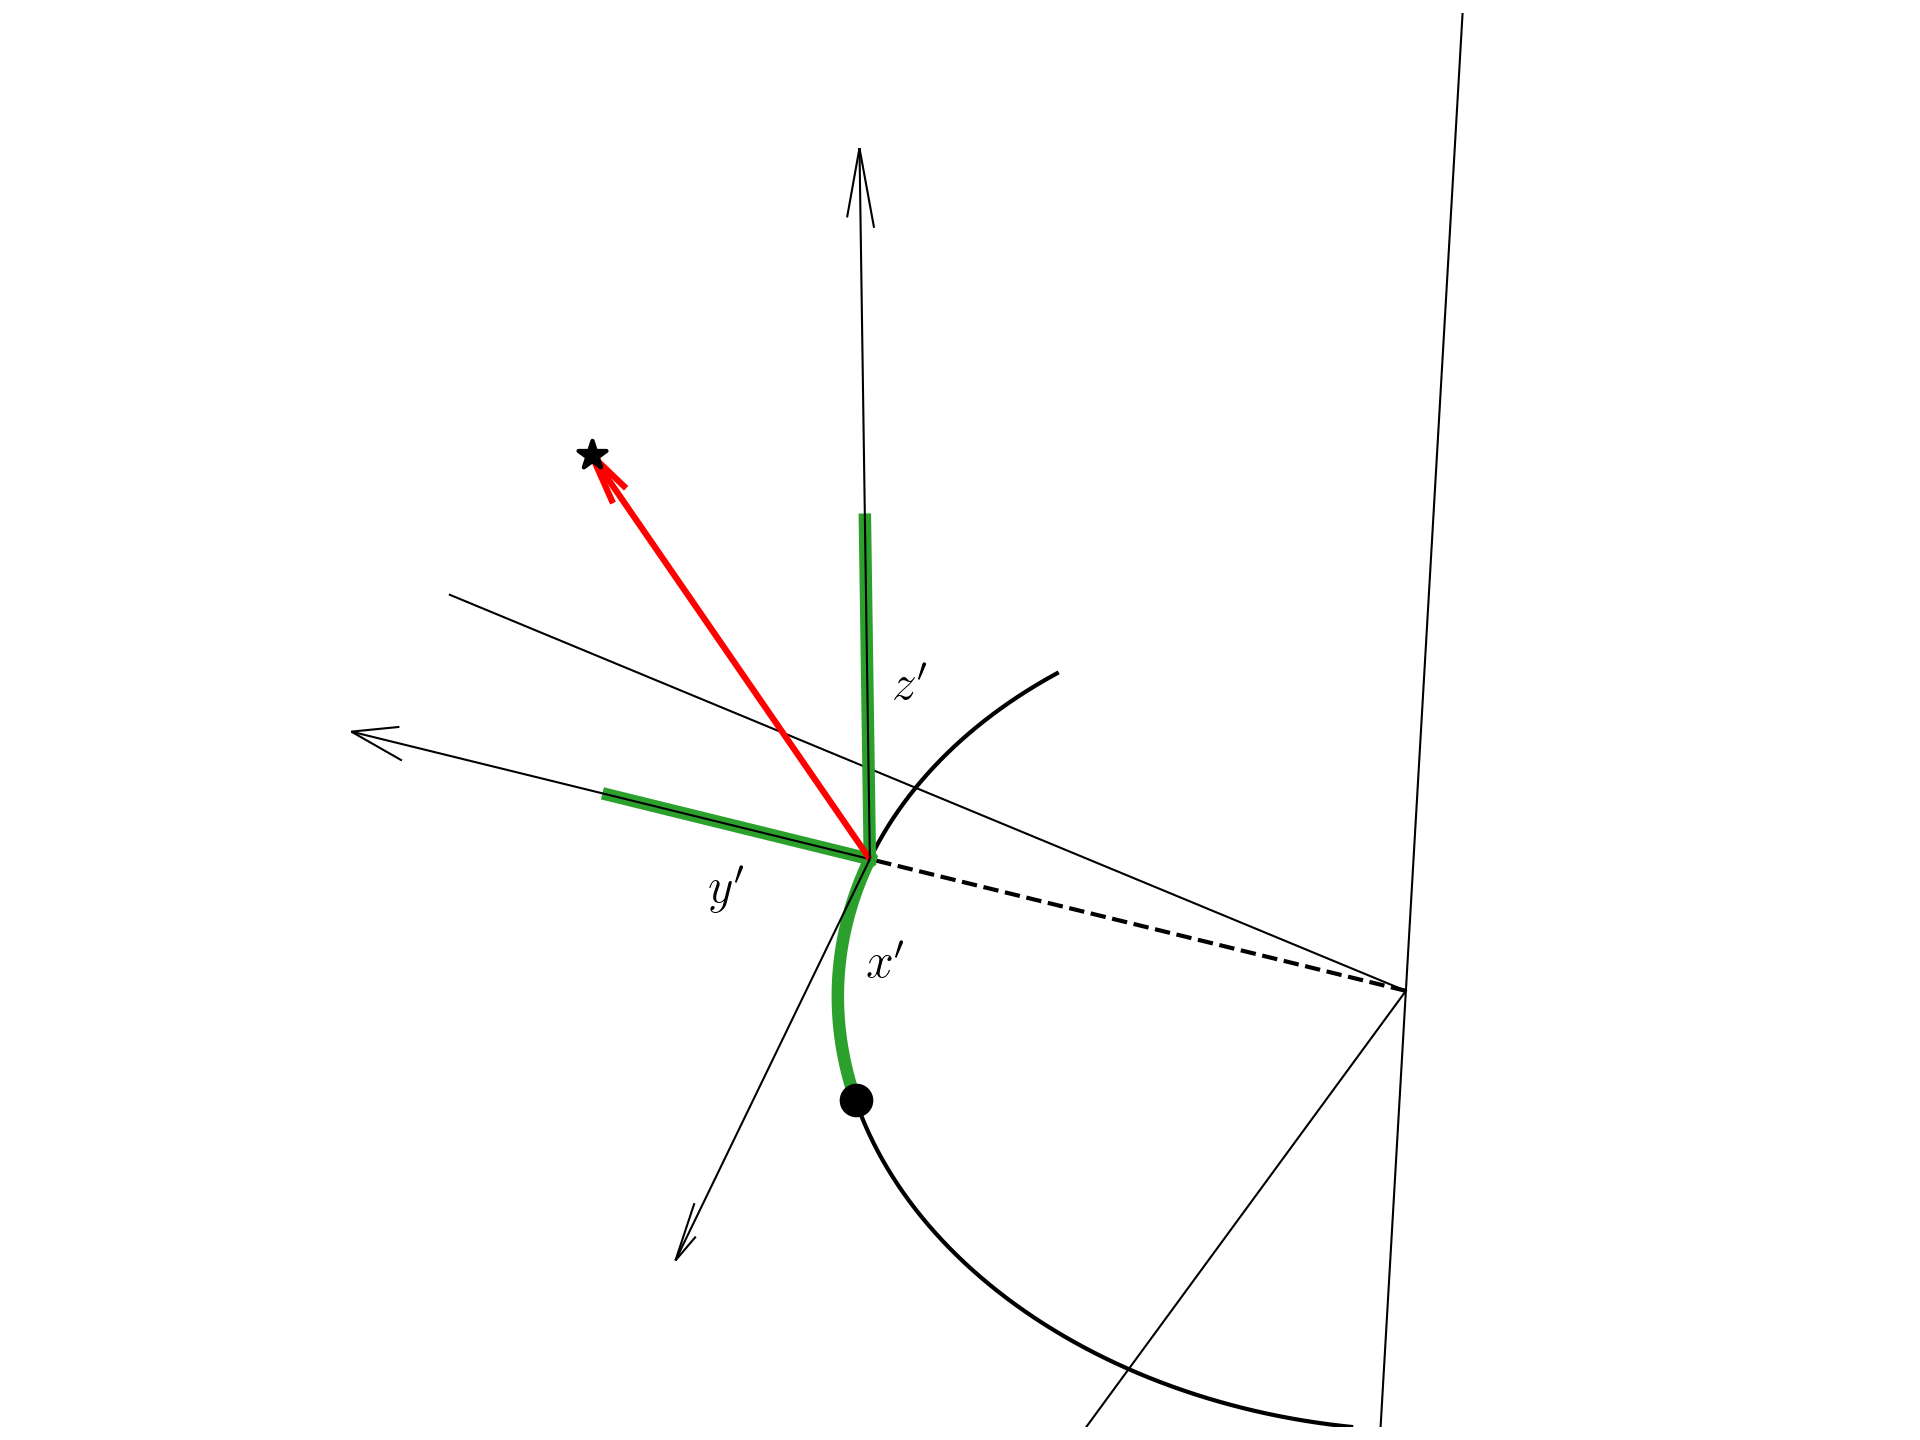
\includegraphics[width=\linewidth]{tailcoordinates.png}
      \caption{A demonstration of the transformation from galactic coordinates to tail coordinates. The black dot represents the globular cluster, while the thick black line shows a segment of its orbit. \DIFdelbeginFL \DIFdelFL{A }\DIFdelendFL \DIFaddbeginFL \DIFaddFL{The }\DIFaddendFL star \DIFdelbeginFL \DIFdelFL{particle is marked with }\DIFdelendFL \DIFaddbeginFL \DIFaddFL{symbol indicates }\DIFaddendFL a star \DIFdelbeginFL \DIFdelFL{symbol}\DIFdelendFL \DIFaddbeginFL \DIFaddFL{particle}\DIFaddendFL . The red vector points from the nearest point on the cluster's orbit to the star particle. \DIFdelbeginFL \DIFdelFL{Its projection onto the }\DIFdelendFL \DIFaddbeginFL \DIFaddFL{The }\DIFaddendFL galactocentric \DIFdelbeginFL \DIFdelFL{unit }\DIFdelendFL \DIFaddbeginFL \DIFaddFL{position }\DIFaddendFL vector is \DIFdelbeginFL \DIFdelFL{shown in green and labeled }\DIFdelendFL \DIFaddbeginFL \DIFaddFL{the }\DIFaddendFL $y'$\DIFaddbeginFL \DIFaddFL{-axis}\DIFaddendFL . The \DIFdelbeginFL \DIFdelFL{red vector is also projected onto }\DIFdelendFL \DIFaddbeginFL \DIFaddFL{local orbital plane, }\DIFaddendFL the \DIFdelbeginFL \DIFdelFL{vector perpendicular to both }\DIFdelendFL \DIFaddbeginFL \DIFaddFL{cross-product between }\DIFaddendFL the \DIFdelbeginFL \DIFdelFL{orbital tangent }\DIFdelendFL \DIFaddbeginFL \DIFaddFL{orbit's local position }\DIFaddendFL and \DIFdelbeginFL \DIFdelFL{the galactocentric }\DIFdelendFL \DIFaddbeginFL \DIFaddFL{velocity }\DIFaddendFL vector, \DIFdelbeginFL \DIFdelFL{which }\DIFdelendFL defines the \DIFdelbeginFL \DIFdelFL{local orbital plane and is labeled }\DIFdelendFL $z'$\DIFaddbeginFL \DIFaddFL{-axis}\DIFaddendFL . \DIFdelbeginFL \DIFdelFL{The }\DIFdelendFL \DIFaddbeginFL \DIFaddFL{We project the red vector on each of these axes. We measure the x' coordinate as the }\DIFaddendFL path length along the orbit from the cluster to the nearest point\DIFdelbeginFL \DIFdelFL{is denoted as }\DIFdelendFL \DIFaddbeginFL \DIFaddFL{. Positive }\DIFaddendFL $x'$, \DIFdelbeginFL \DIFdelFL{with $x'$ being positive if the particle }\DIFdelendFL \DIFaddbeginFL \DIFaddFL{$y'$, $z'$ indicate that a star }\DIFaddendFL is ahead of the cluster\DIFaddbeginFL \DIFaddFL{, farther from the galactic center, and above the orbital plane, respectively}\DIFaddendFL .}
      \label{fig:TailCoordinates}
    \end{figure}

    \begin{figure*}
      \centering
      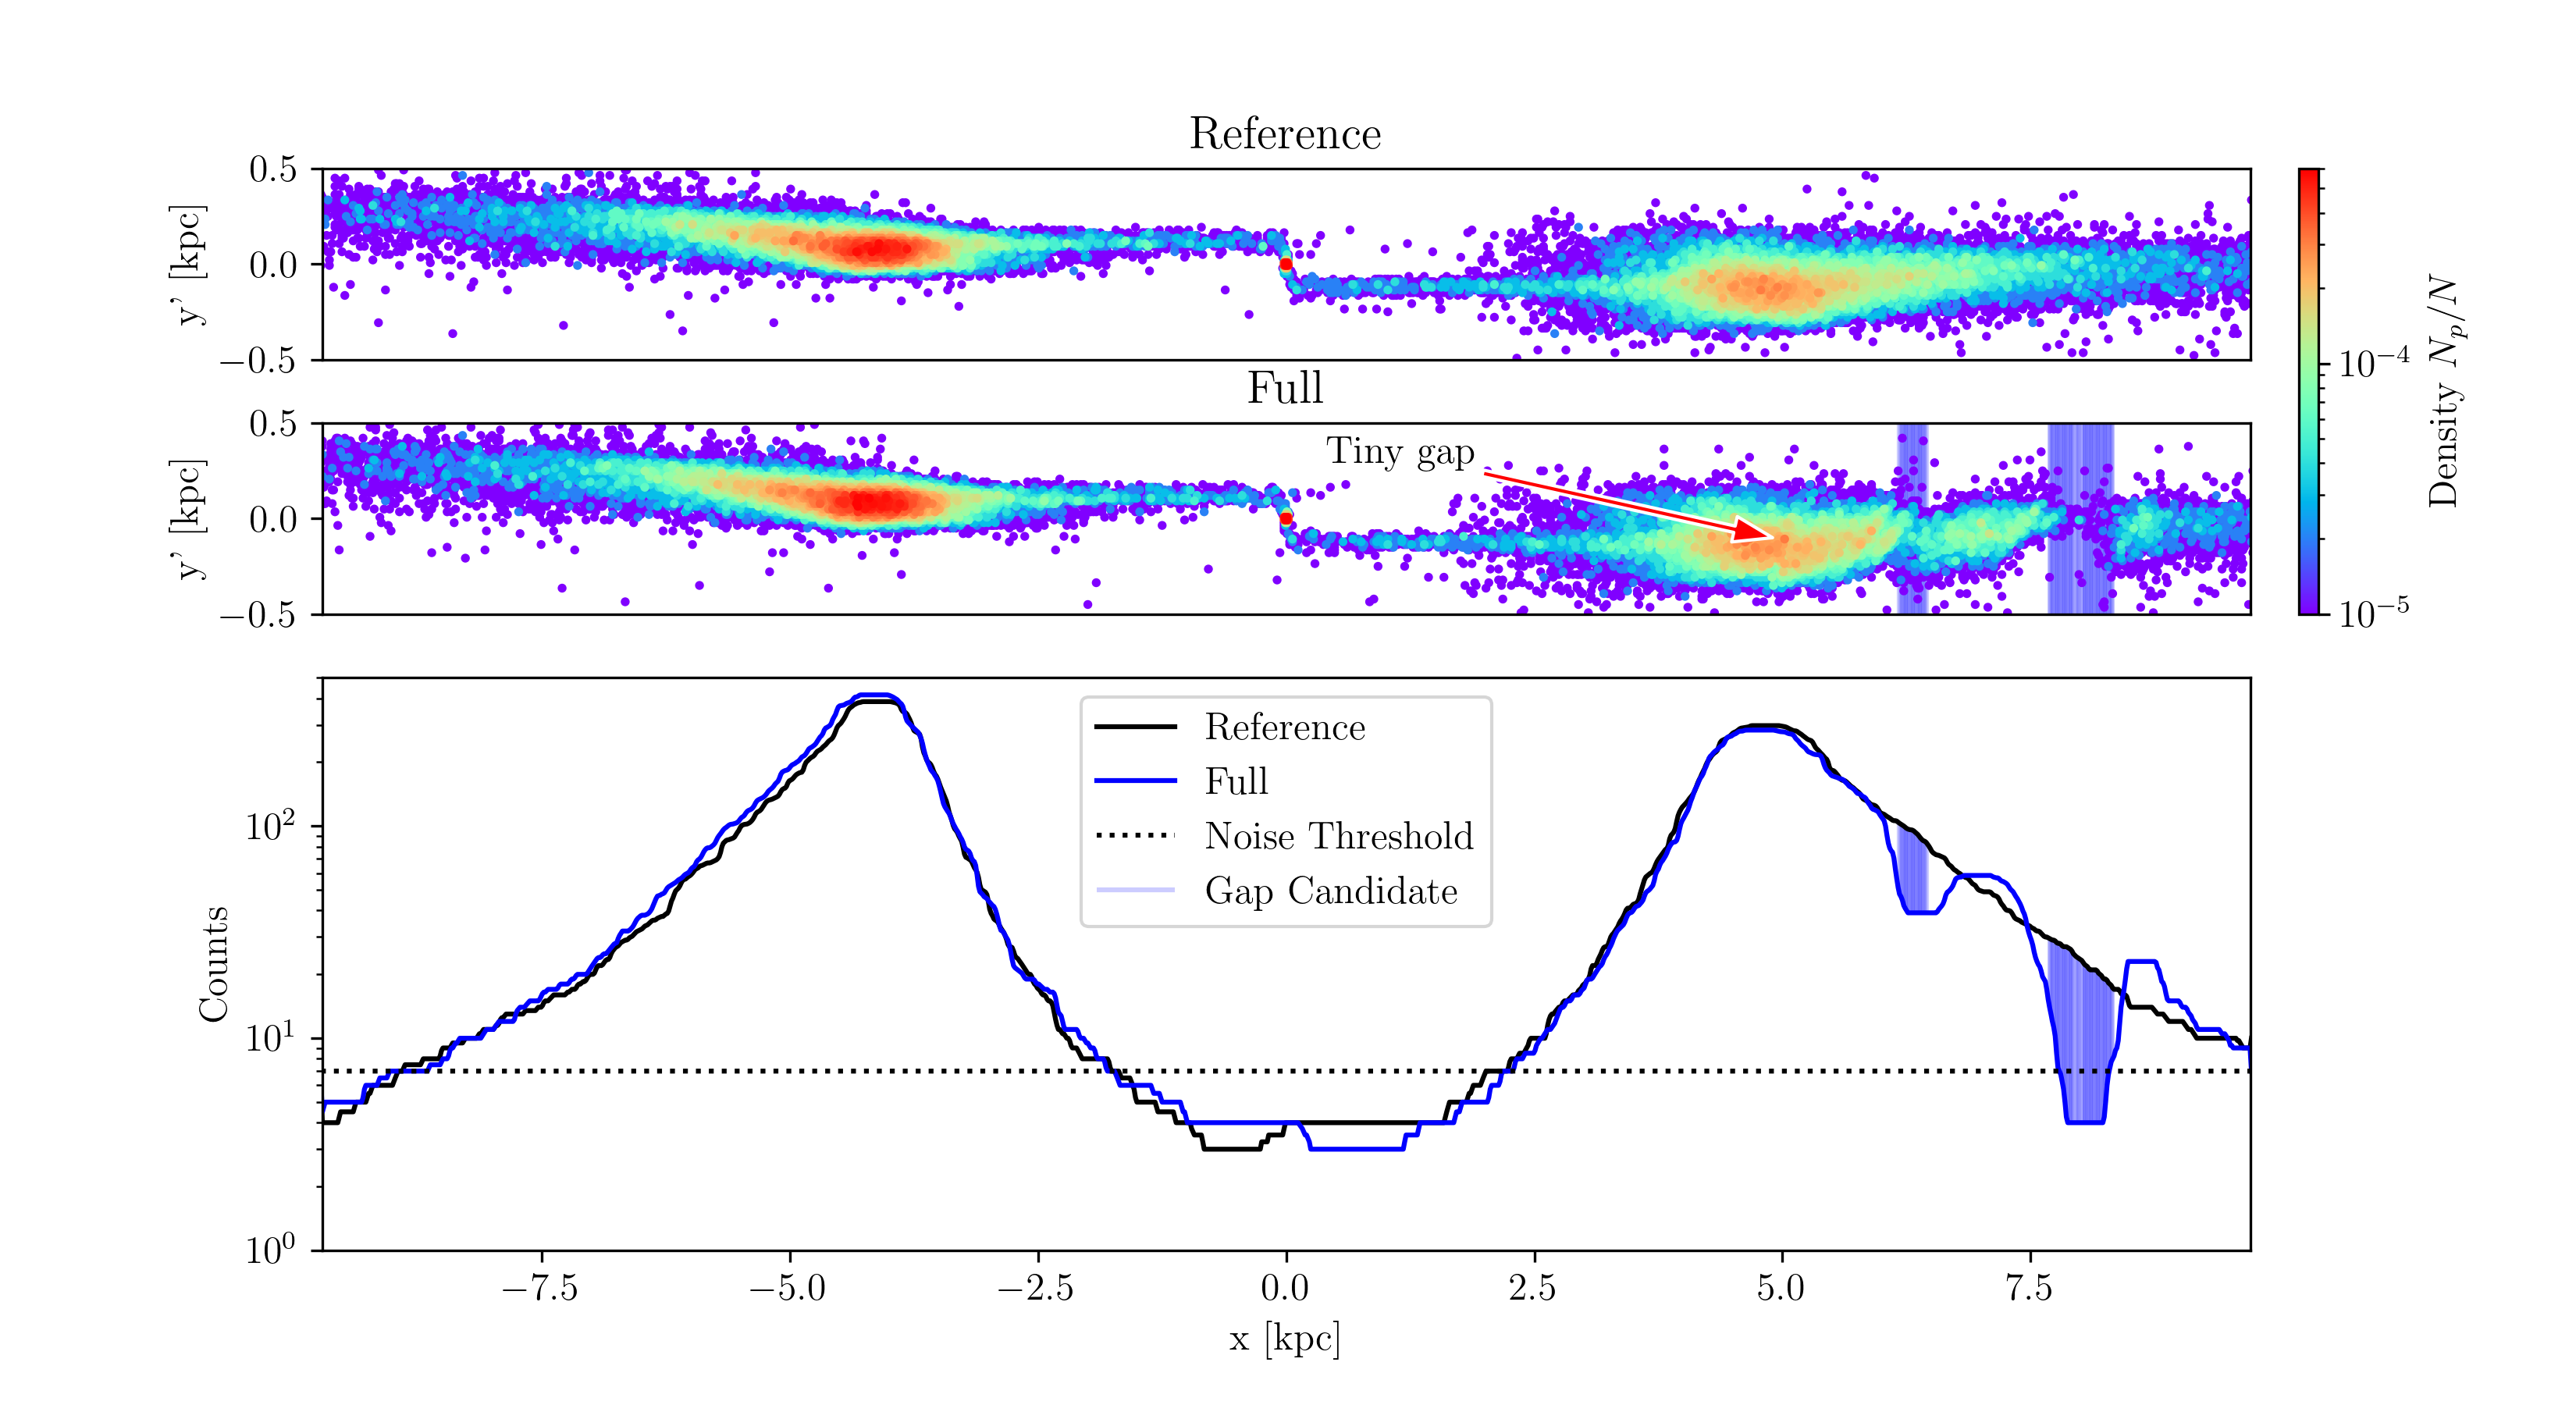
\includegraphics[width=\linewidth, trim=20 0 15 0]{monte-carlo-009-pouliasis2017pii-GCNBody-2000-milisigma-5-noisefactor-20-boxcarindexlength-shifted-0.png}
      \caption{A comparison between the density maps and profiles of the \texttt{full} and \texttt{reference} simulations is presented. The \DIFaddbeginFL \DIFaddFL{blue vertical bars highlight the }\DIFaddendFL locations where the \texttt{full} simulation is less dense than the \texttt{reference} simulation by 2-$\sigma$\DIFdelbeginFL \DIFdelFL{is highlighted by blue vertical bars}\DIFdelendFL . \DIFdelbeginFL \DIFdelFL{Bins }\DIFdelendFL \DIFaddbeginFL \DIFaddFL{We do not consider bins }\DIFaddendFL below the noise threshold \DIFdelbeginFL \DIFdelFL{are not considered }\DIFdelendFL when measuring the differences between the two 1D profiles. \DIFdelbeginFL \DIFdelFL{The }\DIFdelendFL \DIFaddbeginFL \DIFaddFL{We smoothed the }\DIFaddendFL 1D profiles \DIFdelbeginFL \DIFdelFL{have been smoothed }\DIFdelendFL with a median box-car filter.}
      \label{fig:profiles}
      \end{figure*}

    To construct the 1D density profiles, we bin the data using the $\sqrt{N}$ rule, where $N$ is the number of data points ($N_p = 10^5$). After binning the 1D profiles, we apply a \DIFaddbegin \DIFadd{median }\DIFaddend boxcar smoothing technique. \DIFdelbegin \DIFdel{This raw profile density curve is smoothed with the median box-car filter. }\DIFdelend At each bin, \DIFdelbegin \DIFdel{a selected }\DIFdelend \DIFaddbegin \DIFadd{we select a }\DIFaddend number of adjacent data points from both sides\DIFdelbegin \DIFdel{are placed }\DIFdelend \DIFaddbegin \DIFadd{, place them }\DIFaddend in a list\DIFdelbegin \DIFdel{. The bin is then replaced }\DIFdelend \DIFaddbegin \DIFadd{, and replace the central value of the bin }\DIFaddend with the median. We \DIFdelbegin \DIFdel{choose to }\DIFdelend use 10 adjacent points per side, \DIFdelbegin \DIFdel{which correspond }\DIFdelend \DIFaddbegin \DIFadd{corresponding }\DIFaddend to a smoothing length of approximately 1~kpc. This procedure reduces high-frequency noise and smooths the profiles. For instance, notice the absence of a high mass peak indicating \DIFdelbegin \DIFdel{for }\DIFdelend the center of mass in the bottom panel of Fig.~\ref{fig:profiles}.

    With the smoothed 1D density profiles in hand, we search \DIFdelbegin \DIFdel{for }\DIFdelend regions where the \texttt{full} simulations are significantly under-dense compared to \texttt{reference} simulations, surpassing stochastic fluctuations. \DIFdelbegin \DIFdel{To accomplish this, we }\DIFdelend \DIFaddbegin \DIFadd{We }\DIFaddend first impose a signal-to-noise ratio threshold, $\mathcal{SNR}$. The signal is \DIFdelbegin \DIFdel{defined as }\DIFdelend the log of the counts per bin from the \texttt{reference} 1D density profile\DIFdelbegin \DIFdel{, and errors are propagated }\DIFdelend \DIFaddbegin \DIFadd{; we propagate errors }\DIFaddend assuming a Poisson distribution. We then compute a threshold for the number of counts in the \texttt{reference} simulation, $N_v$, using the transcendental equation:
    \begin{equation}
        \mathcal{SNR} = \ln(10) \log_{10}\left(N_v\right) \sqrt{N_v}.
      \end{equation} \label{eq:density_threshold}
    By setting $\mathcal{SNR} = 5$, we solve for $N$ using \texttt{scipy.optimize.fsolve}, finding that $N$ must be greater than 7. After discarding insignificant bins (i.e., those with counts below the threshold), we compute the log ratio of the counts between the \texttt{reference} and \texttt{full} simulations:
    \begin{equation}
        \mathcal{R}_i = \log_{10}\left(\frac{N_{f,i}}{N_{v,i}}\right),
      \end{equation}
    where $\mathcal{R}_i$ is the log ratio, $N_{f,i}$ are the counts from the \texttt{full} simulation, and $N_{v,i}$ are the counts from the \texttt{reference} simulation for each bin $i$. We then analyze the \DIFdelbegin \DIFdel{distribution of }\DIFdelend $\mathcal{R}_i$ \DIFaddbegin \DIFadd{distribution}\DIFaddend . If the differences between the density profiles are primarily due to stochastic processes of similar magnitude, this distribution should resemble a Gaussian\DIFaddbegin \DIFadd{, }\DIFaddend as expected from the central limit theorem. Thus, we flag all regions where the density is \DIFdelbegin \DIFdel{under-dense }\DIFdelend \DIFaddbegin \DIFadd{underdense }\DIFaddend by more than two standard deviations, which should highlight regions whose \DIFdelbegin \DIFdel{under-density }\DIFdelend \DIFaddbegin \DIFadd{underdensity }\DIFaddend is unlikely to be the result of the sum of stochastic processes but rather the passage of another globular cluster. 

    However, this method has its limitations, especially when detecting smaller gaps. As outlined by \citet{2015MNRAS.450.1136E}, \DIFdelbegin \DIFdel{a }\DIFdelend \DIFaddbegin \DIFadd{since gap growth is a dispersion phenomenon, a }\DIFaddend small gap is not indicative of a weak impact \DIFdelbegin \DIFdel{, }\DIFdelend but a recent one. \DIFdelbegin \DIFdel{This is because gap growth is a dispersion phenomenon. }\DIFdelend Additionally, since our streams have finite width, some gaps are oblique with respect to the stream axis. In such cases, marginalizing over $y'$ erases the gap's signal, making it impossible to detect in a 1D profile. This limitation is particularly evident in gaps caused by NGC~2808, as discussed in the results. Therefore, this quantitative analysis serves as an \textit{aid} to visual inspection rather than a complete substitute for it. This method helps \DIFdelbegin \DIFdel{particularly with large subtle gaps that }\DIFdelend \DIFaddbegin \DIFadd{with significant, subtle gaps }\DIFaddend the eye does not notice in the 2D maps. \DIFdelbegin \DIFdel{These profiles are included in the }\DIFdelend Appendix~\ref{sec:gallery_of_gaps} \DIFaddbegin \DIFadd{presents these profiles}\DIFaddend .


  \section{Perturber Identification} \label{sec:Perturber_Identification}

    \DIFdelbegin \DIFdel{A key question we }\DIFdelend \DIFaddbegin \DIFadd{We }\DIFaddend seek to answer \DIFdelbegin \DIFdel{is: from }\DIFdelend \DIFaddbegin \DIFadd{a key question: From }\DIFaddend the gaps present at the end of the simulation, who caused them? To address this, we examine the evolution of stream density over time. Instead of using the x'-coordinate, we introduce $\tau$, which represents time rather than distance. Specifically, $\tau$ indicates how long \DIFdelbegin \DIFdel{it will take for a cluster to reach, }\DIFdelend \DIFaddbegin \DIFadd{a cluster will take to reach a given point in its orbit }\DIFaddend or how long ago it passed\DIFdelbegin \DIFdel{, a given point on its orbit. This }\DIFdelend \DIFaddbegin \DIFadd{. This choice of coordinates }\DIFaddend is advantageous because the growth of the stream is approximately linear in $\tau$\DIFdelbegin \DIFdel{whereas }\DIFdelend \DIFaddbegin \DIFadd{. In contrast, }\DIFaddend in physical space, streams on eccentric orbits expand and contract depending on the orbital phase.


    \citet{2016MNRAS.457.3817S} extended the analysis of \citet{2015MNRAS.450.1136E}, demonstrating that action-angle variables provide a useful coordinate system for analyzing stream evolution, as actions are conserved \DIFdelbegin \DIFdel{and the angles associated with the stream's growth evolve }\DIFdelend \DIFaddbegin \DIFadd{quantities and their associated angles grow }\DIFaddend linearly over time. Although we became aware of this work only after completing our analysis, we note that $\tau$ is a suitable approximation and behaves similarly to the angle variable corresponding to the azimuthal action: \DIFdelbegin \DIFdel{$\tau \approx \theta_{\phi,i} - \theta_{\phi,\text{GC}}$}\DIFdelend \DIFaddbegin \DIFadd{$\tau \approx \theta_{\phi, i} - \theta_{\phi,\text{GC}}$}\DIFaddend .

    The core of our analysis is presented in Fig.~\ref{fig:force-on-orbit}. The bottom panel shows the evolution of the stream density over time. To avoid \DIFdelbegin \DIFdel{extreme }\DIFdelend \DIFaddbegin \DIFadd{extremely }\DIFaddend low-density regions at the stream's edges, we applied the same density threshold as from Eq.~\ref{eq:density_threshold} to focus on the more significant areas of the stream. Next, we modeled Palomar~5's orbit as a proxy for its stream and sampled points along the orbit to measure the gravitational force exerted by other globular clusters. \DIFdelbegin \DIFdel{This force data is displayed in the }\DIFdelend \DIFaddbegin \DIFadd{The }\DIFaddend top panel of Fig.~\ref{fig:force-on-orbit} \DIFdelbegin \DIFdel{, showing }\DIFdelend \DIFaddbegin \DIFadd{shows }\DIFaddend how the total gravitational acceleration on Palomar~5's stream evolves over its length throughout the simulation.

    \begin{figure*}
      \centering
      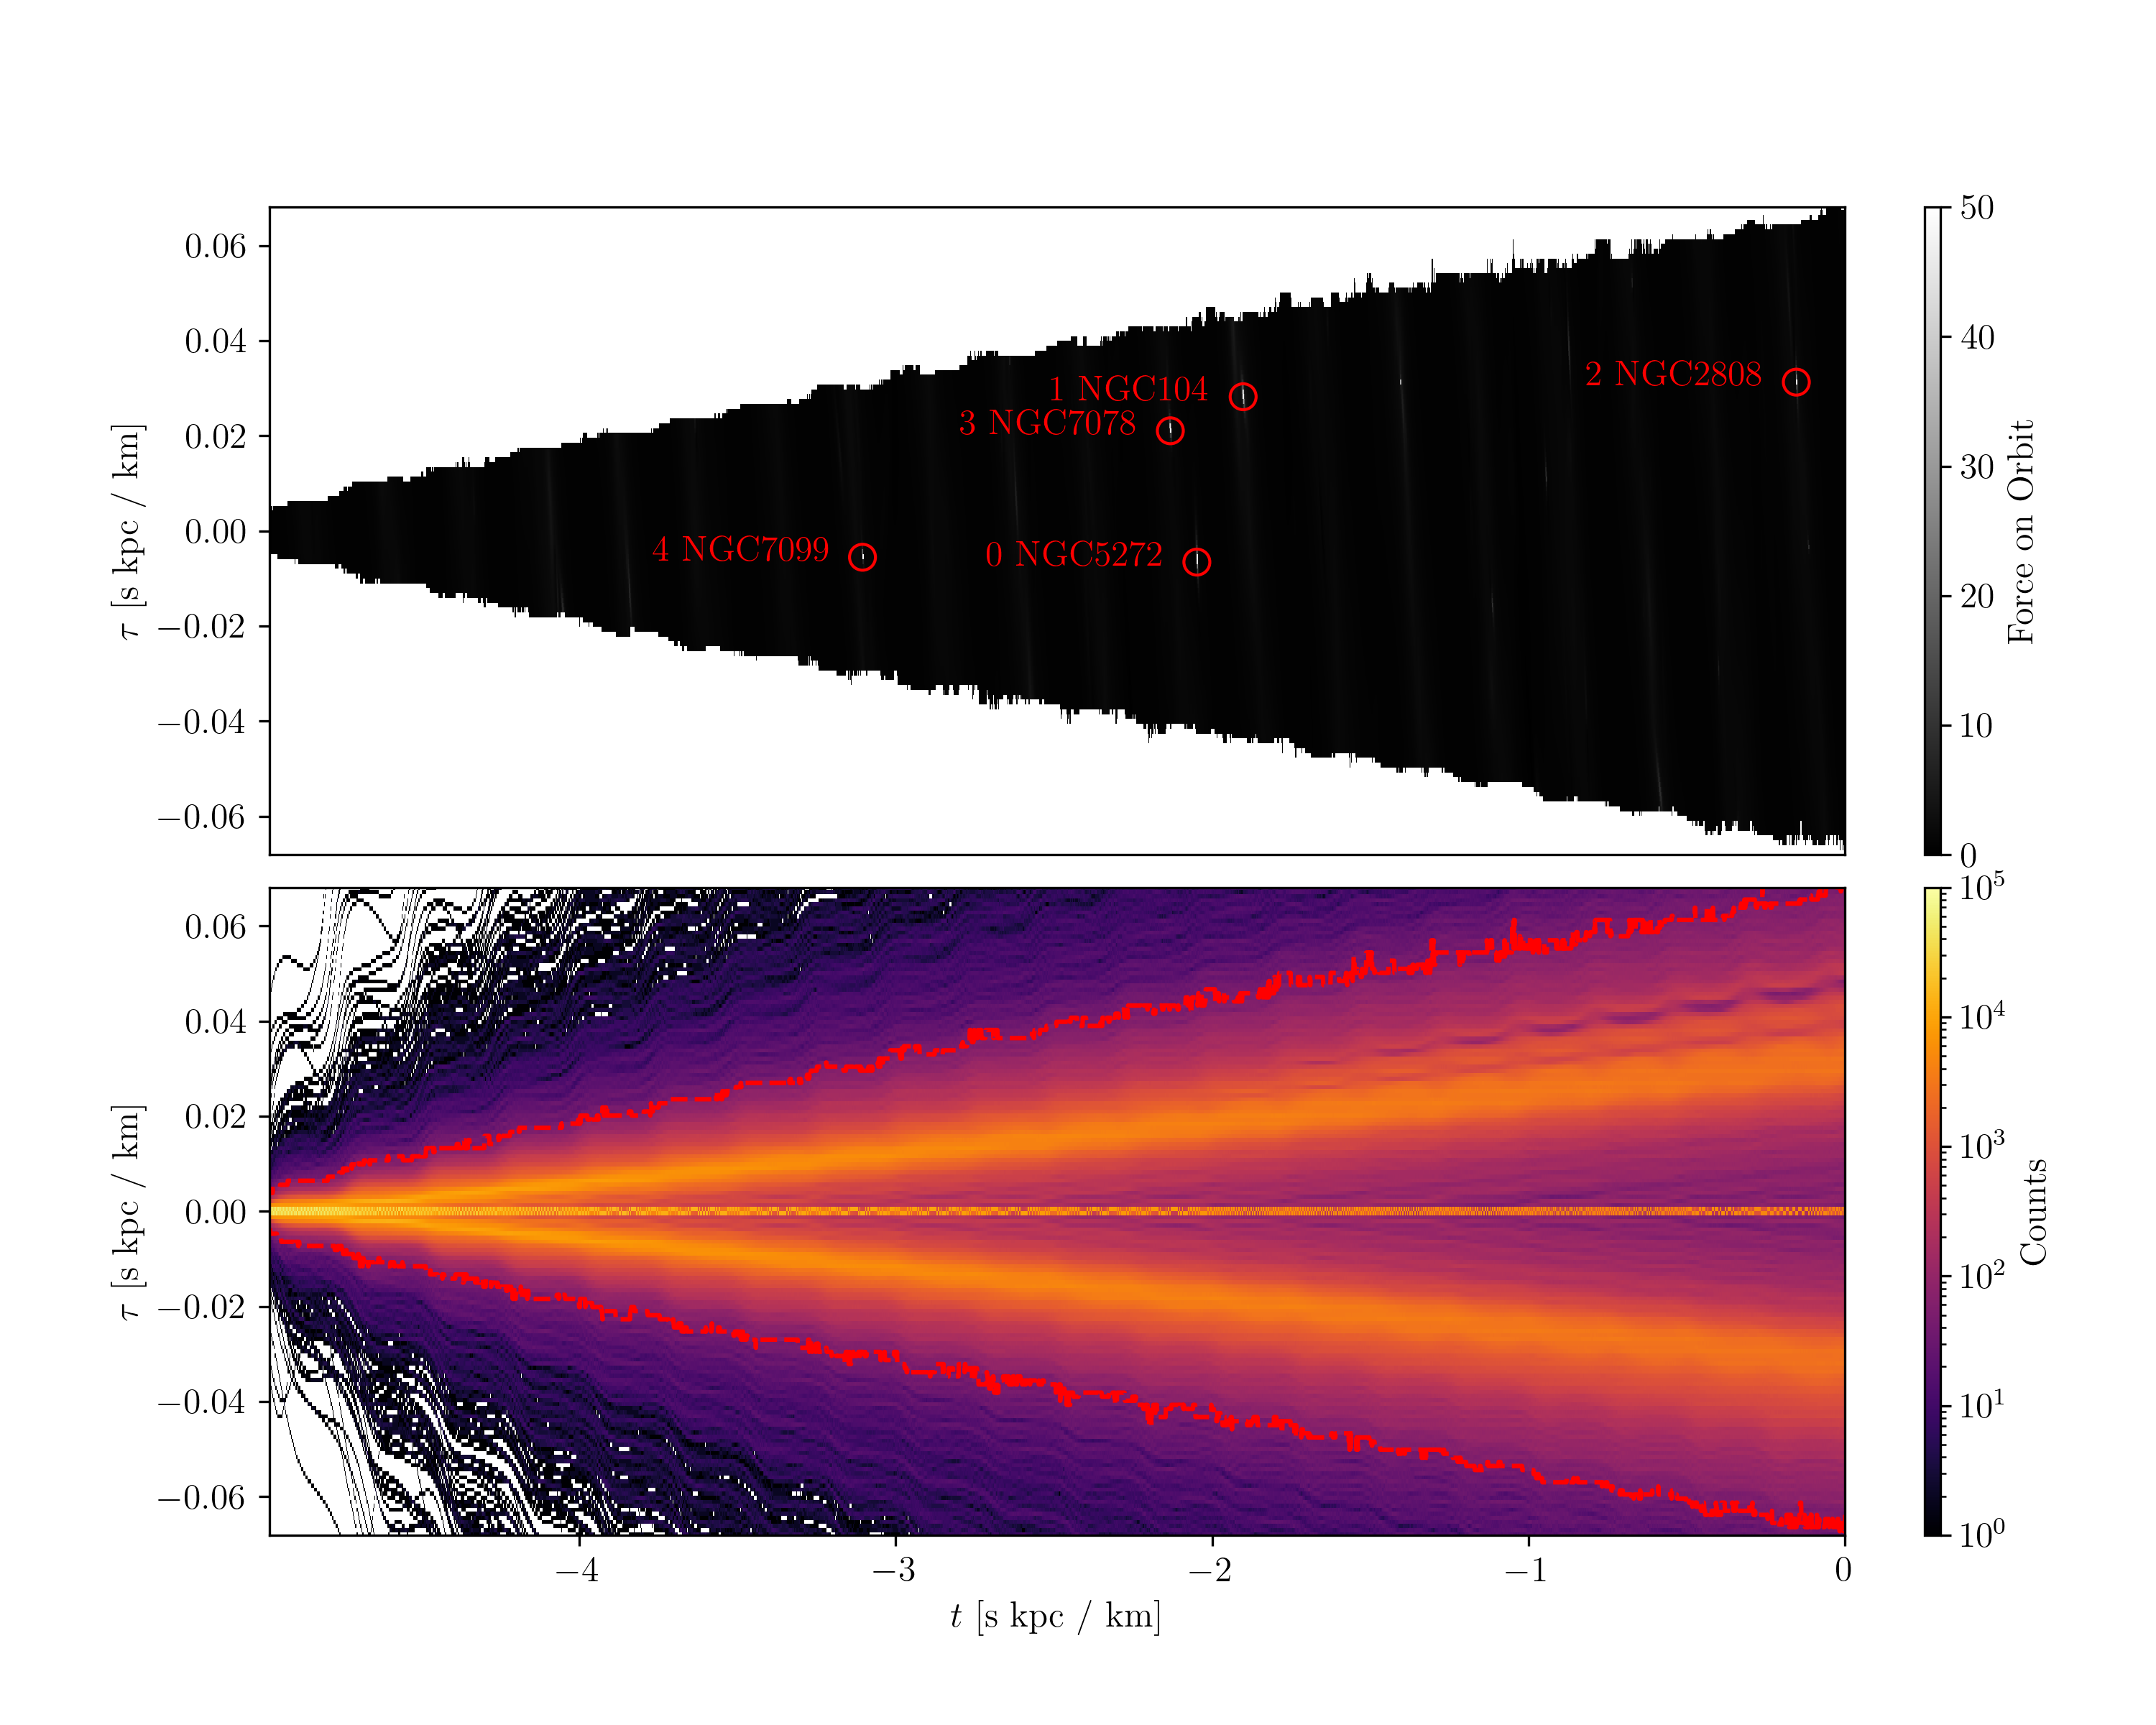
\includegraphics[width=\linewidth]{force_on_orbit-monte-carlo-009.png}
      \caption{This figure demonstrates how we determined which globular clusters were responsible for the gaps. The y-axis is $\tau$, \DIFdelbeginFL \DIFdelFL{which is }\DIFdelendFL a coordinate in units of time that indicates how far ahead or behind it is from a globular cluster. The x-axis is the simulation time, $t$, where 0~s km~kpc$^{-1}$ indicates \DIFaddbeginFL \DIFaddFL{the }\DIFaddendFL present time. The bottom plot showcases the evolution of the stream density \DIFdelbeginFL \DIFdelFL{in }\DIFdelendFL \DIFaddbeginFL \DIFaddFL{over }\DIFaddendFL simulation time. \DIFdelbeginFL \DIFdelFL{The density was }\DIFdelendFL \DIFaddbeginFL \DIFaddFL{We }\DIFaddendFL used \DIFaddbeginFL \DIFaddFL{the density }\DIFaddendFL to determine a suitable \DIFdelbeginFL \DIFdelFL{length of the }\DIFdelendFL stream \DIFdelbeginFL \DIFdelFL{at a given function. This }\DIFdelendFL length\DIFdelbeginFL \DIFdelFL{was then }\DIFdelendFL \DIFaddbeginFL \DIFaddFL{. Subsequently, we }\DIFaddendFL used \DIFaddbeginFL \DIFaddFL{this length }\DIFaddendFL to extract a piece of Palomar~5's orbit. This orbital segment \DIFdelbeginFL \DIFdelFL{is used to approximate }\DIFdelendFL \DIFaddbeginFL \DIFaddFL{approximates }\DIFaddendFL the stream. Then, \DIFaddbeginFL \DIFaddFL{we compute }\DIFaddendFL the gravitational force from all other \DIFaddbeginFL \DIFaddFL{stream stand-in }\DIFaddendFL clusters\DIFdelbeginFL \DIFdelFL{was computed on the orbit. This is }\DIFdelendFL \DIFaddbeginFL \DIFaddFL{, }\DIFaddendFL shown in the top plot\DIFdelbeginFL \DIFdelFL{, where the }\DIFdelendFL \DIFaddbeginFL \DIFaddFL{. The }\DIFaddendFL gravitational force is \DIFdelbeginFL \DIFdelFL{in }\DIFdelendFL measured in acceleration and is given in integration units: km$^2$~kpc$^{-1}$~s$^{-2}$. Moments of high acceleration indicate the passage of another cluster. The \DIFaddbeginFL \DIFaddFL{red circles indicate the }\DIFaddendFL top 5 strongest passages\DIFdelbeginFL \DIFdelFL{are labeled with red circles }\DIFdelendFL \DIFaddbeginFL \DIFaddFL{, }\DIFaddendFL as well as the \DIFdelbeginFL \DIFdelFL{name }\DIFdelendFL \DIFaddbeginFL \DIFaddFL{names }\DIFaddendFL of the clusters. The example shown in this plot is the same simulation as Fig.~\ref{fig:stream_on_sky}.}
      \label{fig:force-on-orbit}
    \end{figure*}  


    We then used \texttt{scipy}'s \texttt{ndimage} \citep{2020NatMe..17..261V} package to identify the top five local maxima in the data space of gravitational acceleration $\vec{g}$ as a function of time $t$ and the stream coordinate $\tau$. \DIFdelbegin \DIFdel{This is done by first smoothing the image }\DIFdelend \DIFaddbegin \DIFadd{First, we smooth the data space }\DIFaddend by taking a \DIFdelbegin \DIFdel{5 point }\DIFdelend \DIFaddbegin \DIFadd{5-point }\DIFaddend moving average kernel. Secondly, we use \DIFaddbegin \DIFadd{a }\DIFaddend maximum filter to locate coordinates in the ($t,\tau$) data plane \DIFdelbegin \DIFdel{who }\DIFdelend \DIFaddbegin \DIFadd{that }\DIFaddend are local maxima to at least \DIFdelbegin \DIFdel{10-adjacent }\DIFdelend \DIFaddbegin \DIFadd{10 adjacent }\DIFaddend data points. \DIFdelbegin \DIFdel{These locations are then ordered and }\DIFdelend \DIFaddbegin \DIFadd{We order these locations and save }\DIFaddend the top five strongest interactions\DIFdelbegin \DIFdel{are saved. Once these local maxima were identified}\DIFdelend \DIFaddbegin \DIFadd{. Then}\DIFaddend , we iterated over the contributions of individual globular clusters to determine which cluster contributed the most to each peak in $\vec{g}$. \DIFdelbegin \DIFdel{Each significant peak was labeled }\DIFdelend \DIFaddbegin \DIFadd{We label each significant peak }\DIFaddend with the corresponding globular cluster.


    Afterward, we cross-referenced these peaks with the locations of the gaps identified by studying the density maps and profiles from Fig.~\ref{fig:profiles}. \DIFdelbegin \DIFdel{For large gaps resulting from strong interactions, we observed that after an impact , }\DIFdelend \DIFaddbegin \DIFadd{The impact leaves }\DIFaddend a low-density wake \DIFdelbegin \DIFdel{is left behind }\DIFdelend in the ($t,\tau$) plane \DIFdelbegin \DIFdel{, which can be seen }\DIFdelend \DIFaddbegin \DIFadd{for large gaps resulting from strong interactions. the bottom panel of Fig.~\ref{fig:force-on-orbit} shows the wakes }\DIFaddend corresponding to the impacts of NGC~104 and NGC~\DIFdelbegin \DIFdel{7808 in the bottom panel of Fig.~\ref{fig:force-on-orbit}.
}\DIFdelend \DIFaddbegin \DIFadd{7808.
}\DIFaddend 



    Fig.~\ref{fig:force-on-orbit} contains some interesting information. Notice the periodic ribbons of force in the $(t,\tau)$ plane. \DIFdelbegin \DIFdel{This is }\DIFdelend \DIFaddbegin \DIFadd{The ribbons are }\DIFaddend due to pericenter passages where Palomar~5 is getting closer to the center of mass of the globular cluster system. Additionally, for the impacts of NGC~104 and NGC~\DIFdelbegin \DIFdel{C7078}\DIFdelend \DIFaddbegin \DIFadd{7078}\DIFaddend , wakes can be observed in the density map. Another important aspect is that the strongest peak in gravitational force does not necessarily create a gap. Notice how NGC~5272, which was labeled with 0 to indicate that it has the greatest local maxima, does not have a gap. The reason for this is manifold\DIFdelbegin \DIFdel{, for }\DIFdelend \DIFaddbegin \DIFadd{. For }\DIFaddend instance, the force needs to be modulated with \DIFdelbegin \DIFdel{the }\DIFdelend time since the change in momentum is the determining factor and not the peak magnitude of the force.  Additionally, there is an offset of about 200~pc between the stream and the orbit, as seen when viewing the stream in tail coordinates, so peaks upon the orbit are good proxies for the stream but are not definitive. We found that the top five greatest impacts accounted for all gaps, except for Sampling~014 as shown in Fig.~\ref{fig:gallery3}, whose gap from NGC~6584 corresponded to the 7th peak. 

    \DIFdelbegin \DIFdel{The }\DIFdelend \DIFaddbegin \DIFadd{We compile the }\DIFaddend results of this analysis \DIFdelbegin \DIFdel{were compiled }\DIFdelend into a table. \DIFdelbegin \DIFdel{If a gap was attributed to a particular globular cluster, it was }\DIFdelend \DIFaddbegin \DIFadd{Each row of the table corresponds to a gap; its corresponding suspects are the columns. The culprit is }\DIFaddend labeled as \texttt{TRUE}\DIFdelbegin \DIFdel{; otherwise, it was marked as }\texttt{\DIFdel{FALSE}}%DIFAUXCMD
\DIFdelend . For a handful of simulations, to \DIFdelbegin \DIFdel{double check that the verdict made correctly when passing from suspect to culprit, we re-compute the simulations}\DIFdelend \DIFaddbegin \DIFadd{double-check that we make the correct verdict, we recompute the simulations, }\DIFaddend yet individually adding one globular cluster at a time. As a result, we \DIFdelbegin \DIFdel{are able to }\DIFdelend \DIFaddbegin \DIFadd{can }\DIFaddend confirm that singular gaps arise from the suspected clusters\DIFdelbegin \DIFdel{, an example of which is shown in }\DIFdelend \DIFaddbegin \DIFadd{. }\DIFaddend Fig.~\ref{fig:decomposition} \DIFaddbegin \DIFadd{shows one such example}\DIFaddend . 



    \section{Reconstruction of the impact geometry} \label{sec:reconstruction}

    As discussed in Sect~\ref{sect:geometry},  five parameters determine the change in velocity of a given stream particle: $M$, $r_p$, $b$, $W_\parallel$, and $W_\perp$. In the following, we describe how we estimated these parameters during impacts in our simulations.
    To achieve this, we \DIFdelbegin \DIFdel{begin by identifying the approximate moments of impact from }\DIFdelend \DIFaddbegin \DIFadd{identify the impact of }\DIFaddend the most significant clusters, as determined in the previous analysis in Sec.~\ref{sec:Perturber_Identification}. Then, we refine these estimates \DIFdelbegin \DIFdel{in order to to pinpoint both }\DIFdelend \DIFaddbegin \DIFadd{to pinpoint }\DIFaddend the exact location of the impact along the stream and the precise moment it occurred. To do so, we fit a third-order parametric polynomial to the stream \DIFdelbegin \DIFdel{, }\DIFdelend using the saved snapshots from our simulations:
      \begin{equation}
        \vec{s}(\tau) = 
        \left\{
          \begin{aligned}
            x(\tau) &= a_0 + a_1 \tau + a_2 \tau^2 + a_3 \tau^3 \\ 
            y(\tau) &= b_0 + b_1 \tau + b_2 \tau^2 + b_3 \tau^3 \\
            z(\tau) &= c_0 + c_1 \tau + c_2 \tau^2 + c_3 \tau^3
          \end{aligned}
        \right.
        \end{equation}  
      where $x$, $y$, and $z$ represent the parametric line describing the stream in galactocentric coordinates, $\tau$ is the stream coordinate in time as described in the Appendix~\ref{sec:Perturber_Identification}, and is used as the independent variable to parameterize the position along the stream. The coefficients $a_i$, $b_i$, and $c_i$ are the polynomial coefficients. We found that a second-order polynomial was insufficient to capture the curvature along the full length of the stream, with divergence at the ends of the tails. A third-order polynomial was sufficient and desirable, as \DIFdelbegin \DIFdel{it is }\DIFdelend the lowest order \DIFdelbegin \DIFdel{that }\DIFdelend adequately captures the \DIFdelbegin \DIFdel{path of the stream}\DIFdelend \DIFaddbegin \DIFadd{stream's path }\DIFaddend over the entire length under consideration.

      In this analysis, \DIFdelbegin \DIFdel{only }\DIFdelend \DIFaddbegin \DIFadd{we only consider }\DIFaddend one side of the stream\DIFdelbegin \DIFdel{is considered}\DIFdelend . For instance, if the impact candidate was in the leading tail, only the star particles with $\tau > 0$ are used to constrain the stream track. The polynomial coefficients were determined through a minimization method using the Nelder-Mead algorithm from \texttt{scipy}'s optimization package.

      Since \DIFaddbegin \DIFadd{we saved }\DIFaddend the simulation snapshots \DIFdelbegin \DIFdel{were saved }\DIFdelend at a temporal resolution of 1\DIFdelbegin \DIFdel{Myr--—rather }\DIFdelend \DIFaddbegin \DIFadd{~Myr--rather }\DIFaddend than at the integration time-step, which would have generated \DIFdelbegin \DIFdel{an excessive amount of data—--we }\DIFdelend \DIFaddbegin \DIFadd{excessive data, we must }\DIFaddend interpolate between snapshots to more precisely estimate the impact geometry. \DIFdelbegin \DIFdel{This is achieved by fitting the streamat five time-steps }\DIFdelend \DIFaddbegin \DIFadd{We fit the stream's shape with a parametric third-order polynomial at the five time steps }\DIFaddend surrounding the approximate impact time\DIFdelbegin \DIFdel{, }\DIFdelend \DIFaddbegin \DIFadd{. This time is }\DIFaddend a period of 5\DIFdelbegin \DIFdel{Myr, which sufficiently covers }\DIFdelend \DIFaddbegin \DIFadd{~Myr, sufficiently covering }\DIFaddend the interaction time. The interaction time can be estimated as $t \approx \frac{100~\text{pc}}{300~\frac{\text{km}}{\text{s}}} \approx 0.3~\text{Myr}$.

      \DIFdelbegin \DIFdel{As a result, }\DIFdelend \DIFaddbegin \DIFadd{Then, we use a cubic spline interpolation for the coefficients describing the stream's shape, which allows us to describe }\DIFaddend each polynomial coefficient \DIFdelbegin \DIFdel{can now be expressed }\DIFdelend as a function of time. Consequently, we can parameterize the stream as a function of both simulation time and position along the stream:
      \begin{equation}
        \vec{s}(t,\tau) = 
        \left\{
        \begin{aligned}
          x(t,\tau) &= a_0(t) + a_1(t)\tau + a_2(t) \tau^2 + a_3(t)\tau^3 \\ 
          y(t,\tau) &= b_0(t) + b_1(t)\tau + b_2(t) \tau^2 + b_3(t)\tau^3 \\
          z(t,\tau) &= c_0(t) + c_1(t)\tau + c_2(t) \tau^2 + c_3(t)\tau^3.
          \end{aligned}
        \right.
      \end{equation}
      The values of the coefficients as a function of time are obtained through linear interpolation, ensuring that the coefficients at the snapshot times match the values constrained by the simulation data.

      Next, we fit the trajectory of the perturber with a second-order polynomial. With equations for both the stream and the perturber as functions of time, we identify the time and location of impact by minimizing a cost function, defined as the distance between the stream and the perturber:
      \begin{equation} 
        b(t, \tau) = \left\lVert \vec{s}(t, \tau) - \vec{p}(t) \right\rVert, 
        \end{equation}
      \DIFdelbegin \DIFdel{where }\DIFdelend \DIFaddbegin \DIFadd{Where }\DIFaddend $\vec{s}(t, \tau)$ is the galactocentric position of a point on the stream, $\vec{p}(t)$ is the position of the perturber, and $b$ is the distance between the two. The minimum value of $b$, denoted as $\text{min}(b)$, represents the impact parameter. \DIFdelbegin \DIFdel{The minimization is carried out }\DIFdelend \DIFaddbegin \DIFadd{We perform the minimization }\DIFaddend using \texttt{scipy}'s optimization package with the \textit{L-BFGS-B} method, which allows us to place bounds on $t$ and $\tau$, ensuring no extrapolation occurs \citep{davidon1991variable}.

      Once this minimization is \DIFdelbegin \DIFdel{performed}\DIFdelend \DIFaddbegin \DIFadd{done}\DIFaddend , determining the relative velocity becomes straightforward. Since the minimization provides the impact parameter, time of impact, and \DIFaddbegin \DIFadd{the }\DIFaddend corresponding value of $\tau$, we can compute the derivatives of the parametric equations at $t_{\text{min}}$ and $\tau_{\text{min}}$. The parallel and perpendicular components of the perturber's velocity relative to the stream are given by:
      \begin{equation}
        \begin{aligned}
          \delta \vec{v} &=\vec{v_p} - \vec{v_s} \\
          w_\parallel &= \left(\delta \vec{v}\right)\cdot \hat{v_s}\\  
          w_\perp &=  \sqrt{\Delta v ^2 - w_\parallel ^ 2}
          \end{aligned}
        \end{equation}
      where $\vec{v}_p$ and $\vec{v}_s$ are the velocities of the perturber and the stream, respectively. \DIFdelbegin \DIFdel{For each of the }\DIFdelend \DIFaddbegin \DIFadd{We compute the strongest five flybys for each of the }\DIFaddend 50 \DIFdelbegin \DIFdel{simulations, this information was computed for the strongest 5 flybys of a perturber with the stream}\DIFdelend \DIFaddbegin \DIFadd{simulations}\DIFaddend . Thus, we \DIFdelbegin \DIFdel{compute }\DIFdelend \DIFaddbegin \DIFadd{created }\DIFaddend a sample of 250 impacts \DIFdelbegin \DIFdel{, and flag }\DIFdelend \DIFaddbegin \DIFadd{and flagged }\DIFaddend those that give rise to gaps. We refer the reader to Sect.~\ref{sect:geometry} for the presentation and discussion of the results.



\DIFaddbegin \section{\DIFadd{Survival of gaps in streams emerging from more massive globular clusters}}\label{sec:gaps_vs_gcmass}

    \DIFadd{In Section~\ref{sec:mass_loss}, we emphasized that the conditions chosen to simulate the formation and evolution of streams around Pal~5 are probably unrealistic. By choosing, as we did, the same values for the mass and size of the cluster 5 billion years ago as the cluster has today, we did not take into account the loss of mass and internal evolution of the cluster over time. In particular, the velocity dispersion of the stars in a cluster and the velocity dispersion of the stars leaving the cluster and entering the stream depend on the cluster's mass. It is therefore legitimate to ask whether, using a progenitor with a different mass and/or size, the gaps survive and whether, in particular, gaps formed several billion years ago can still be visible today. 
}

  \begin{figure*}
      \centering
      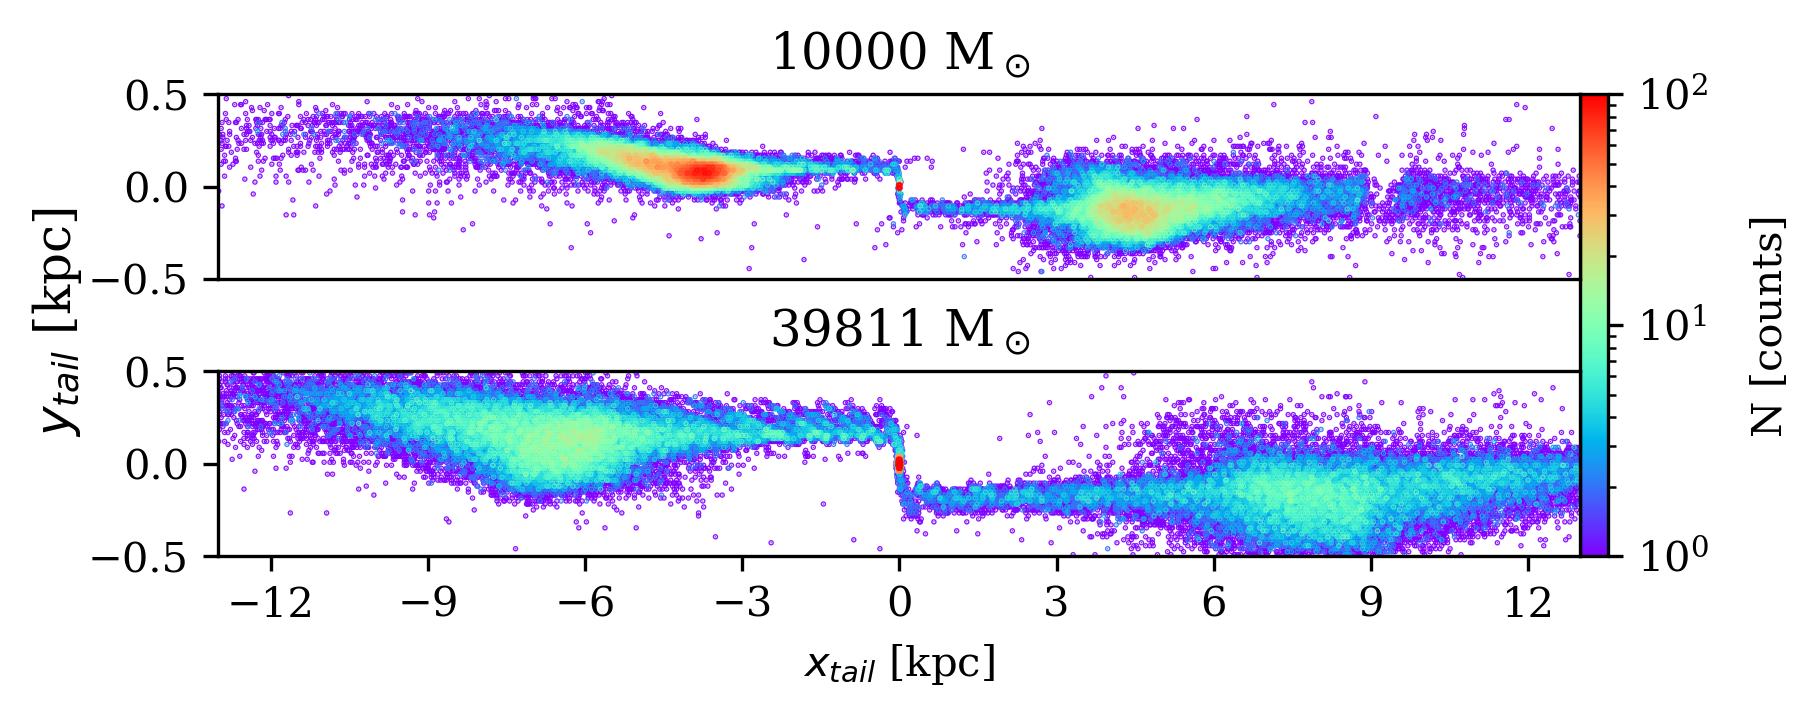
\includegraphics[width=1\linewidth]{gap_no_more.png}
      \caption{\DIFaddFL{When the mass of Palomar~5 is increased, the gap is lost.}}
      \label{fig:gap_no_more}
  \end{figure*}

  \DIFadd{While we anticipate that a specific study on this aspect is in preparation (Ferrone et al, in prep), we would like to preview a few results here. Fig.~\ref{fig:gap_no_more} shows two streams with the same orbital parameters that were impacted by NGC~7078. The top panel shows a stream that comes from a host mass of $10,000$~$M_\odot$, while in the second panel we increased the mass to $\sim40,000$~$M_\odot$. For simplicity, both clusters have the same half-mass radius of 27~pc. The encounter occurred about two and a half billion years ago by NGC~7078, which has a mass of $5.16\times10^{5}~M_\odot$. The gap persists for the lighter host, yet is barely visible in the case of the more massive host. 
}

  \DIFadd{Fig.~\ref{fig:decoherence_shocked_outflow} dissects the more massive stream of Fig.~\ref{fig:gap_no_more} and instructs us why the gap does not persist. The bottom panel shows the total density distribution, and dissects it into two profiles: stars that either are }\textit{\DIFadd{leaked}} \DIFadd{or }\textit{\DIFadd{shocked}} \DIFadd{out of the cluster. By shocked, we mean the stars that are lost during pericenter passages. Tidal forces generally scale with $r^{-3}$, thus significantly strengthening through their pericenter passages. See Fig.~3 of \mbox{%DIFAUXCMD
\citet{2004AJ....127.2753D} }\hskip0pt%DIFAUXCMD
for an illustration of the magnitude of the tidal forces along an orbit. A consequence of the pericenter passages is that many more stars escape, fleeing with a higher mean velocity and velocity dispersion, which can be visualized in the }\textit{\DIFadd{Christmas tree}} \DIFadd{illustration in Fig.~A.3 of \mbox{%DIFAUXCMD
\citet{2012A&A...546L...7M}}\hskip0pt%DIFAUXCMD
. We consider the continous outflow of stars between pericenter passages to be }\textit{\DIFadd{leaked}} \DIFadd{stars. We identify pericenter passages by computing each local minimum of the cluster's galactic-centric 3D radius with }\texttt{\DIFadd{scipy.signal.find\_peaks}}\DIFadd{. The duration of each shock is: $t_{\textrm{shock}}$ = 2$\sqrt{r/|\nabla\Phi|}$, where $r$ is the galactocentric radius and $|\nabla\Phi|$ is the magnitude of the acceleration from the galactic potential. Stars within this range about a given pericenter passage are all given the same color and shown as individual groups in the first, second, third, and fourth panels of Fig.~\ref{fig:decoherence_shocked_outflow}.
}


  \DIFadd{Each group can be simplified as one-dimensional collisionless dispersion. These packets of stars can be described as a population with the same initial position that drifts about a mean velocity, $\langle v \rangle$, with velocity dispersion, $\sigma_v$. The density evolution is a Gaussian whose amplitude decreases inversely with time, and whose standard deviation grows linearly with time:
  }\begin{equation}    
          \DIFadd{\rho(x,t) = \frac{1}{\sigma_v t \sqrt{2\pi} }\textrm{exp}\left(-\frac{1}{2}\left(\frac{x-\langle v \rangle t}{\sigma_v t}\right)^2\right).
  }\end{equation}

  \DIFadd{It is important to note that within a single packet, the stars self-segregate. The position of the density peak is at $\langle v \rangle t$, while the faster stars are ahead and the slower ones are behind. The packets are separated by a distance of $\langle  v\rangle T$, where $T$ is the orbital period. Regarding our simulations, since the mass and radius of the host are held constant, the mean velocity and velocity dispersion are the same across all packets. Secondly, the density of each packet decreases since the easier-to-remove stars are stripped early on. 
}

  \DIFadd{Consider an impact that happens at $x\prime$. The distance from the impact site to each packet is: $\delta x= x\prime - \langle v\rangle \left(t-n T\right)$, where $n$ is the packet index, with $n=0$ being the first packet escaped at the first pericenter passage in the simulation. Note that $\delta x\propto n$, and velocity segregation means $v\propto x$. Therefore, the different parts of the separate packets are hit at a given impact site. The earlier packets are hit in regions where the stars have lower velocities than the later packets. As a result, the gaps in the later packets quickly overtake those from the earlier packets. As a result, the gaps across the packets go out of phase and interfere destructively.
}

  \DIFadd{In the simplest consideration, of two gaps of the same dimension $\sigma_x$ and an offset of $\delta x$, the gaps are out of phase when the separation is greater than the width: $1<\sigma_x/\delta x$. In the temporal analysis of the stream presented in Fig.~\ref{fig:decoherence_shocked_outflow}, we did not observe at any point of the simulation that the gap initially persisted to then go out of phase. Drawing from the wisdom in \mbox{%DIFAUXCMD
\citet{2015MNRAS.450.1136E} }\hskip0pt%DIFAUXCMD
\& \mbox{%DIFAUXCMD
\citet{2016MNRAS.457.3817S}}\hskip0pt%DIFAUXCMD
, we see the contrast between the density peaks and the density minimum of a gap, as well as the width, grow in time, somewhere between $\propto \sqrt{t}$ and linear. In this simplified 1D collisionless dispersion analysis, the gaps between the different packets space apart linearly in time with $\delta x\propto \delta vt$, where $\delta v$ is the mean velocity of the about the impact site for two different packets. This inclines us to believe that the gaps space apart before they become significantly deep or wide, however this need not be the general case. 
}

  \DIFadd{Nonetheless, we believe this is the first consideration of decomposing the stream into packets of tidal bursts to understand the effect of the internal dynamics on gap persistence. Since gap persistence depends on the mass and internal evolution of the cluster, characterizing the gap can constrain our knowledge of the internal evolution. 
}


  \begin{figure}
      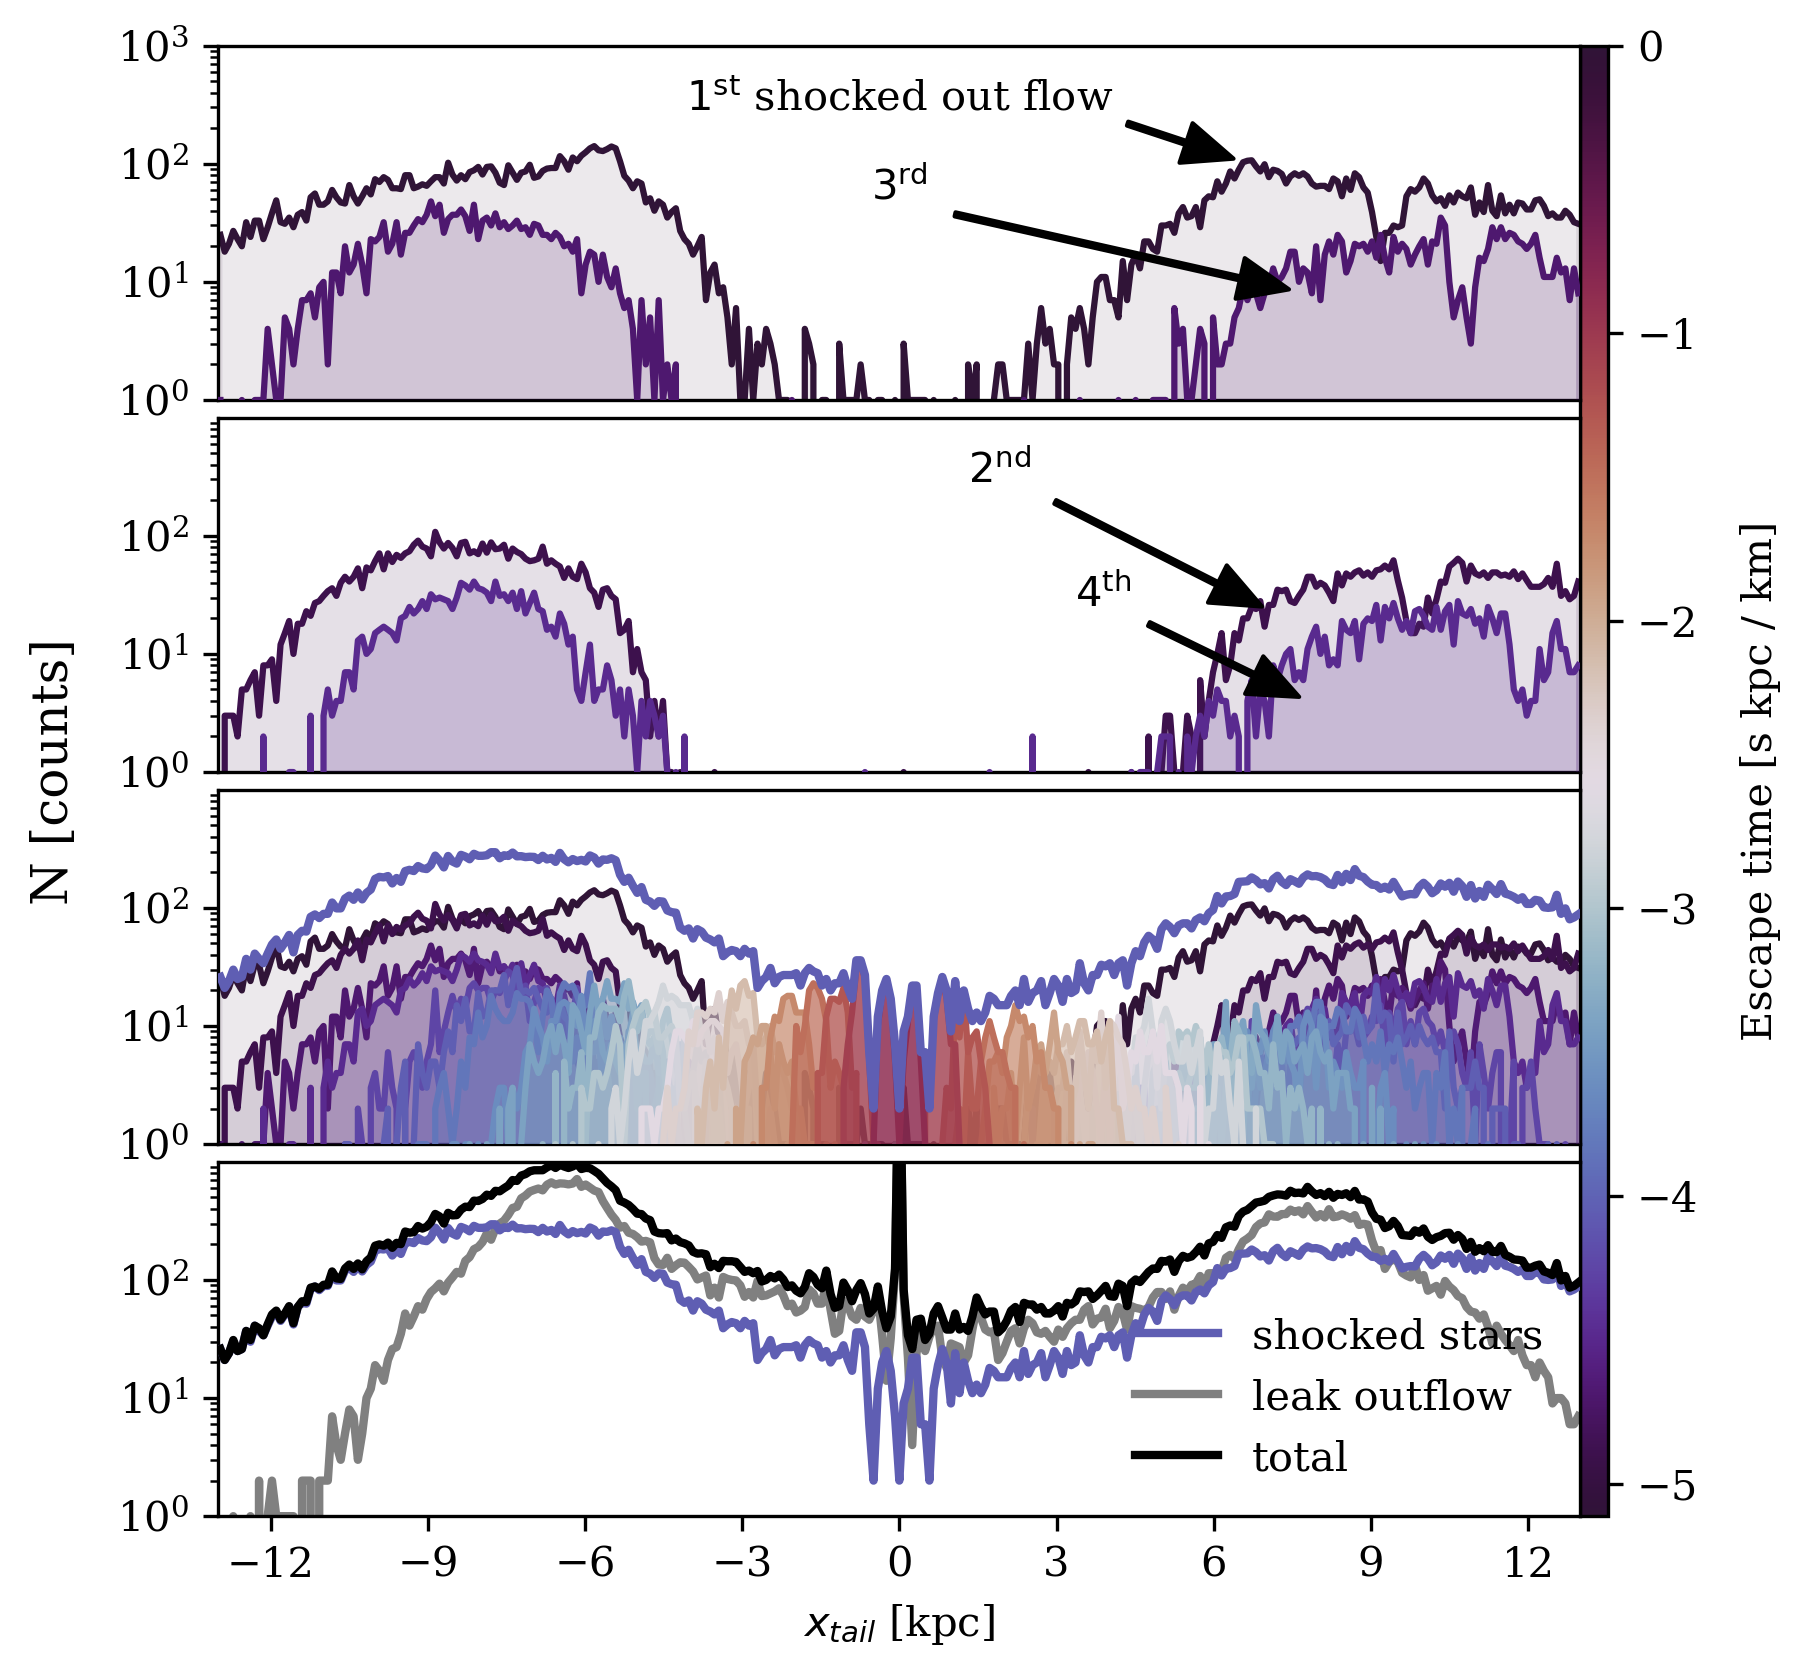
\includegraphics[width=\linewidth]{decoherence_shocked_outflow.png}
      \caption{\DIFaddFL{We dissect the one-dimensional density of the stream from the bottom panel of Fig.~\ref{fig:gap_no_more}. We divide the stars into two categories: the multiple groups that are shocked out at different pericenter passages, or those that leak out of the cluster continuously. The bottom panel shows the leaked population in blue, and each group that was shocked out at each pericenter passage is color-coded by the escape time. The sum of the leaked and shocked outflow gives the total profile density, which is shown in black. The top four panels display the first shocked groups from different pericenter passages, shown individually. Each group shows the gap resulting from the impact of NGC~7078 $\sim$2.5~Gyr ago, yet they are progressively offset as explained in the text.}}
      \label{fig:decoherence_shocked_outflow}
  \end{figure}



  \DIFaddend \section{Gallery of Gaps} \label{sec:gallery_of_gaps}
    Figures~\ref{fig:gallery0}-\ref{fig:gallery11} include all of the realizations of the \texttt{full} simulations of Palomar~5 in tail coordinates. \DIFdelbegin \DIFdel{If a gapis present, it is indicated by a red arrow with }\DIFdelend \DIFaddbegin \DIFadd{A red arrow aids the reader in identifying the gap, accompanied by }\DIFaddend the responsible globular cluster. For the gaps that are not easily visible, we show the 1D profiles showing the significant under-densities compared to the \texttt{reference} simulations. For instance, the second and last panels of Fig.~\ref{fig:gallery0}. However, \DIFdelbegin \DIFdel{maginalizing }\DIFdelend \DIFaddbegin \DIFadd{marginalizing }\DIFaddend the 2D distribution to 1D can erase the signal of oblique gaps. Thus, not all gaps \DIFdelbegin \DIFdel{that are visible }\DIFdelend in the 2D space are \DIFdelbegin \DIFdel{flagged }\DIFdelend \DIFaddbegin \DIFadd{visible }\DIFaddend in the density profiles. For example, in \texttt{Sampling 000}, the gaps from NGC~2808 and NGC~5634 are not flagged \DIFaddbegin \DIFadd{as }\DIFaddend present in the marginalized density profile.

    \begin{figure*}
      \centering
      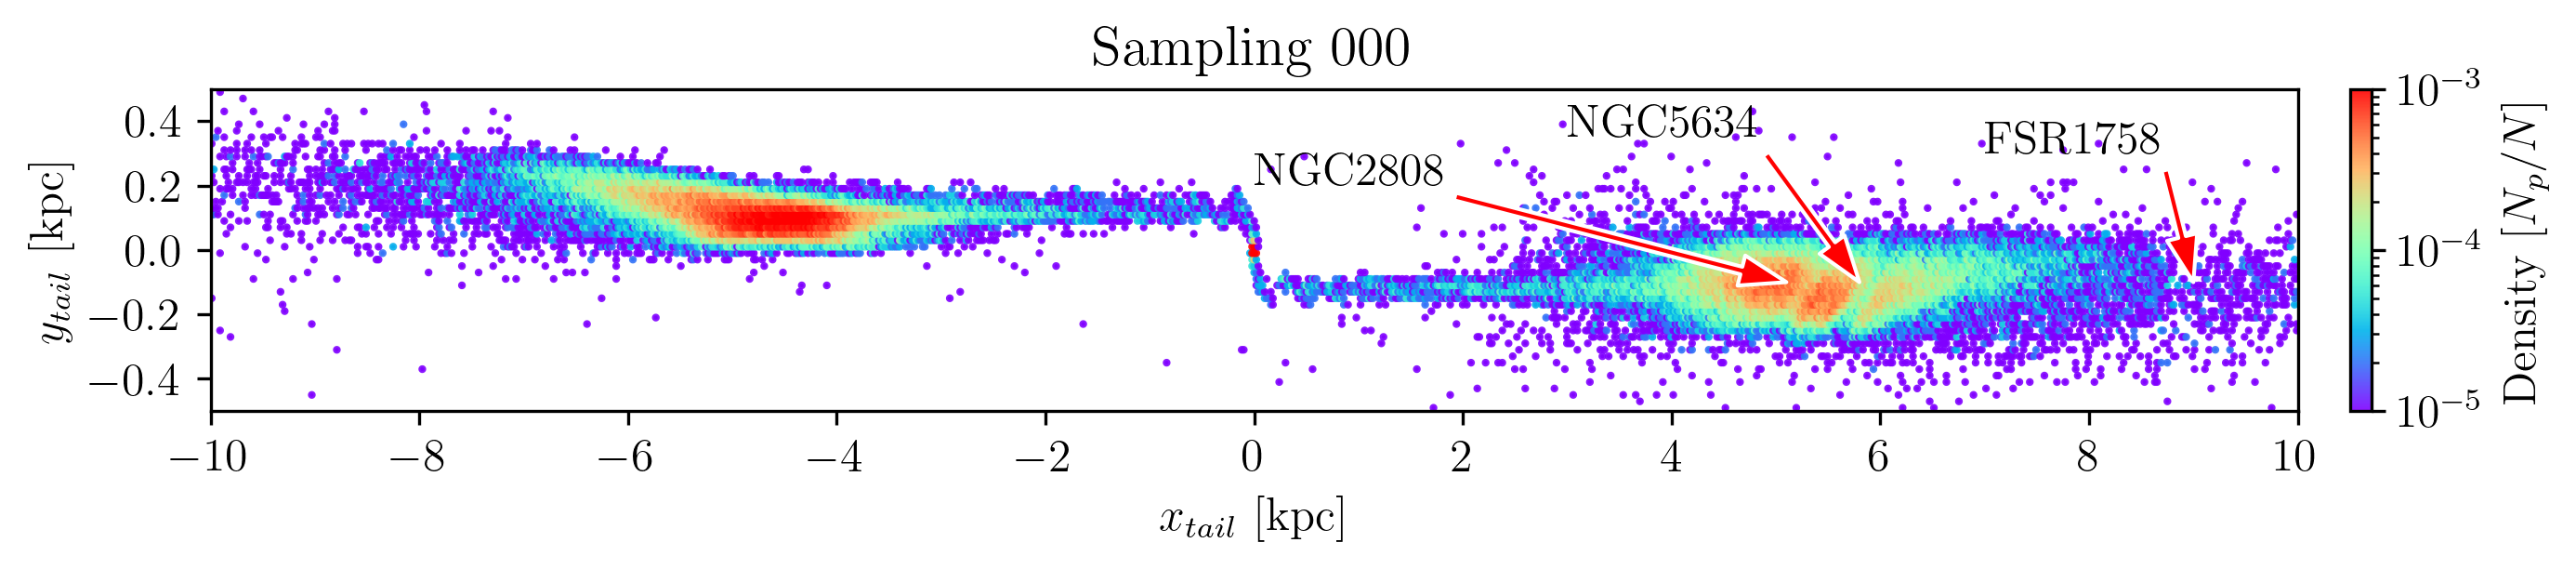
\includegraphics[width=\linewidth]{gallery_of_gaps_monte-carlo-000.png}
      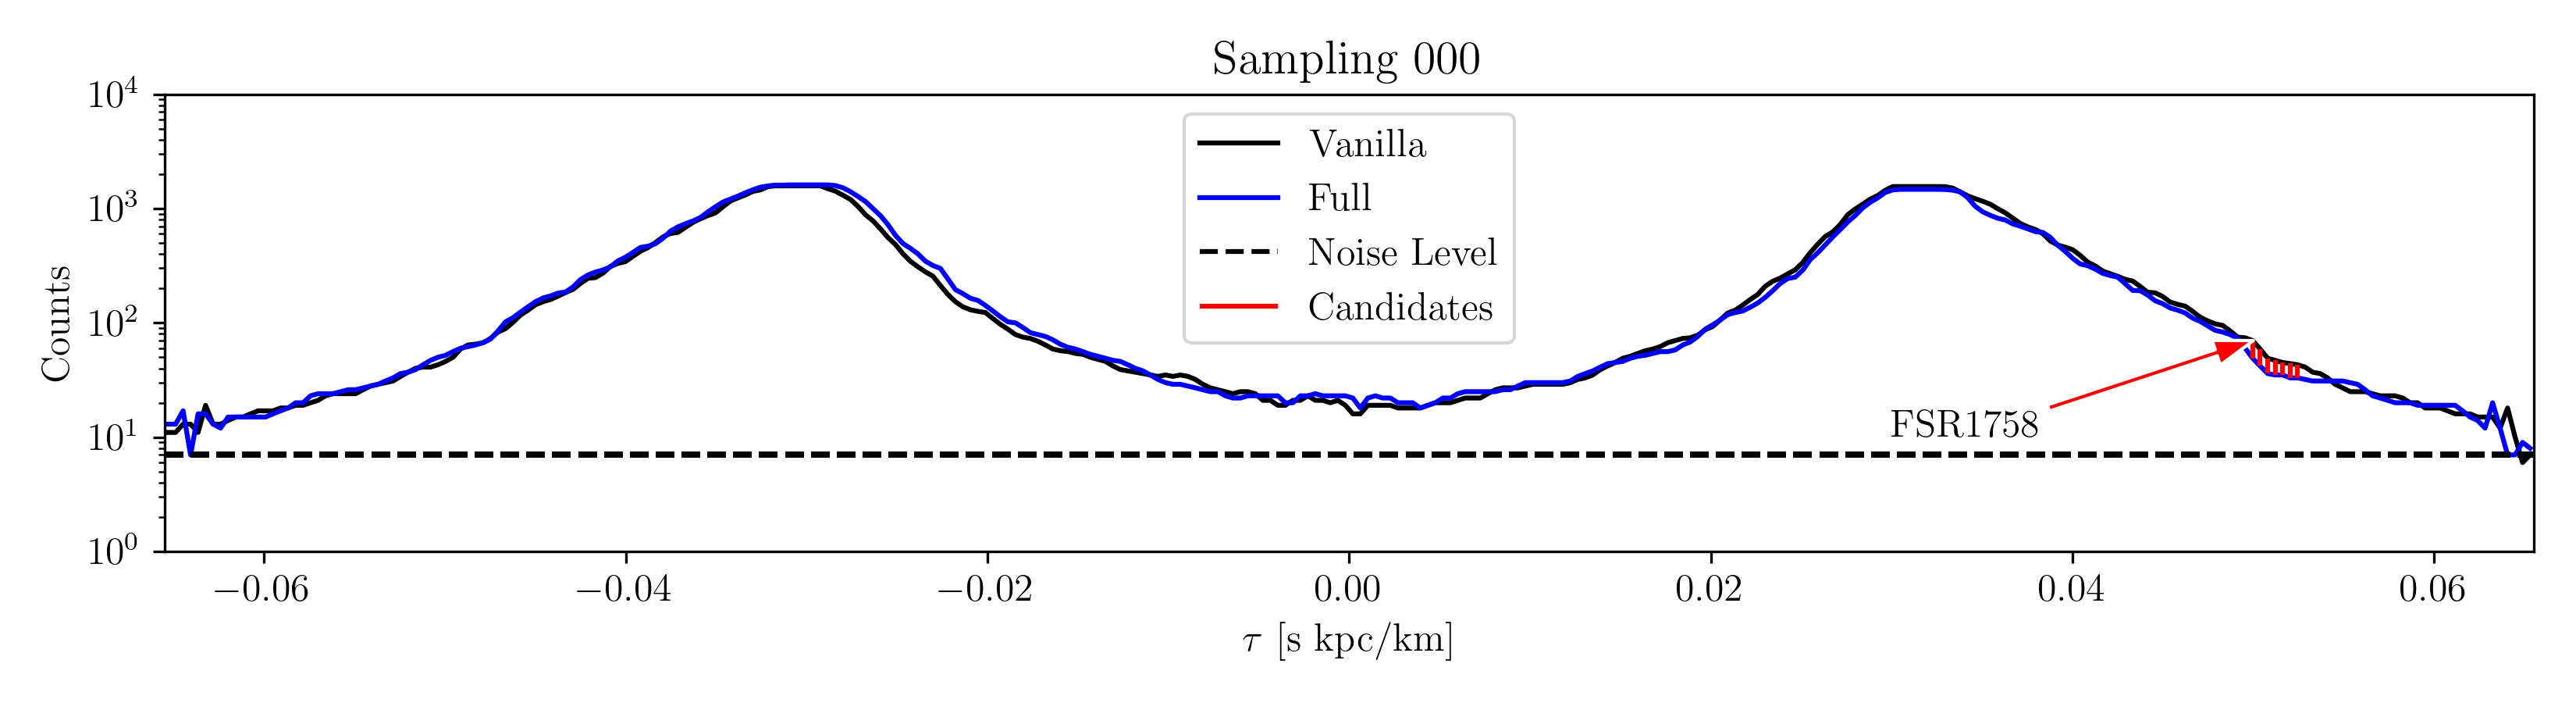
\includegraphics[width=\linewidth]{tau-profile-monte-carlo-000.png}
      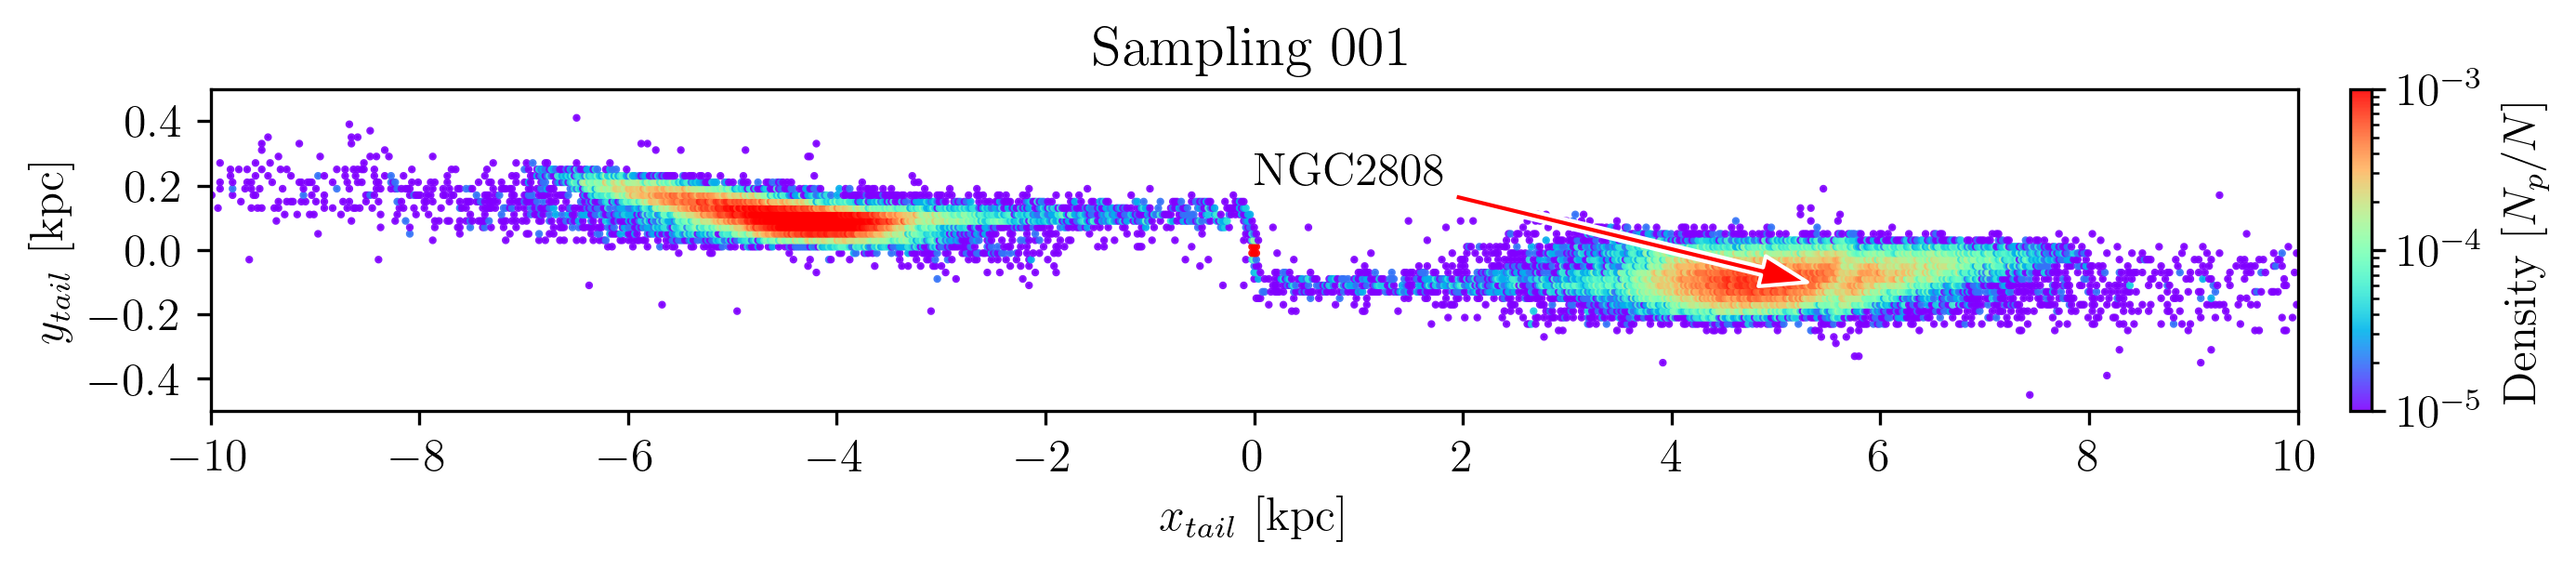
\includegraphics[width=\linewidth]{gallery_of_gaps_monte-carlo-001.png}
      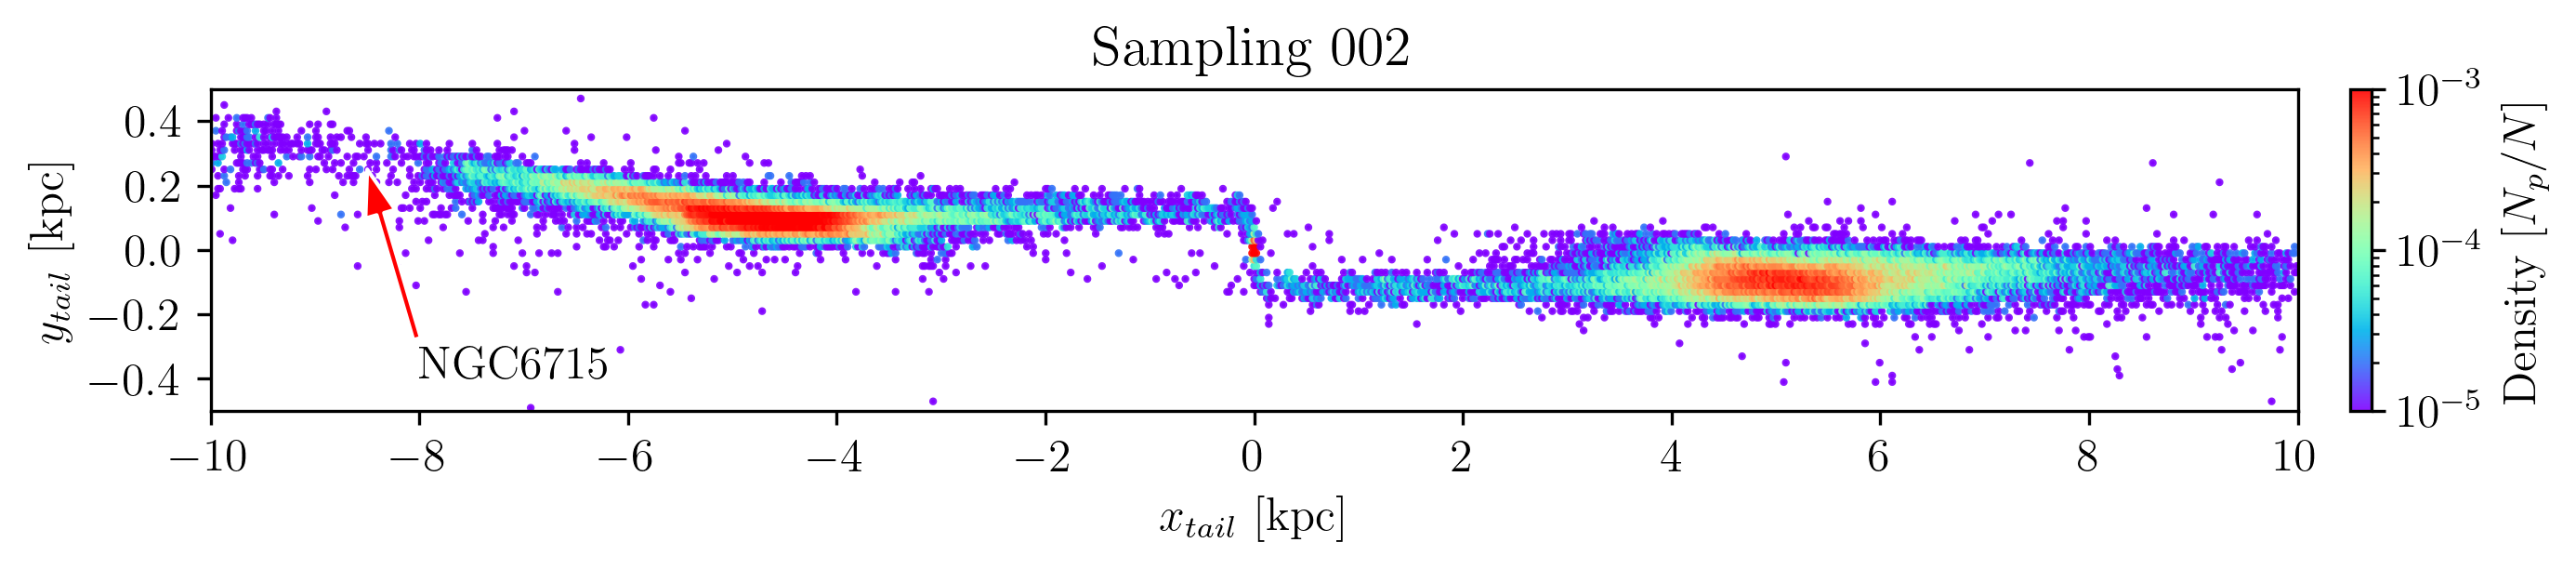
\includegraphics[width=\linewidth]{gallery_of_gaps_monte-carlo-002.png}
      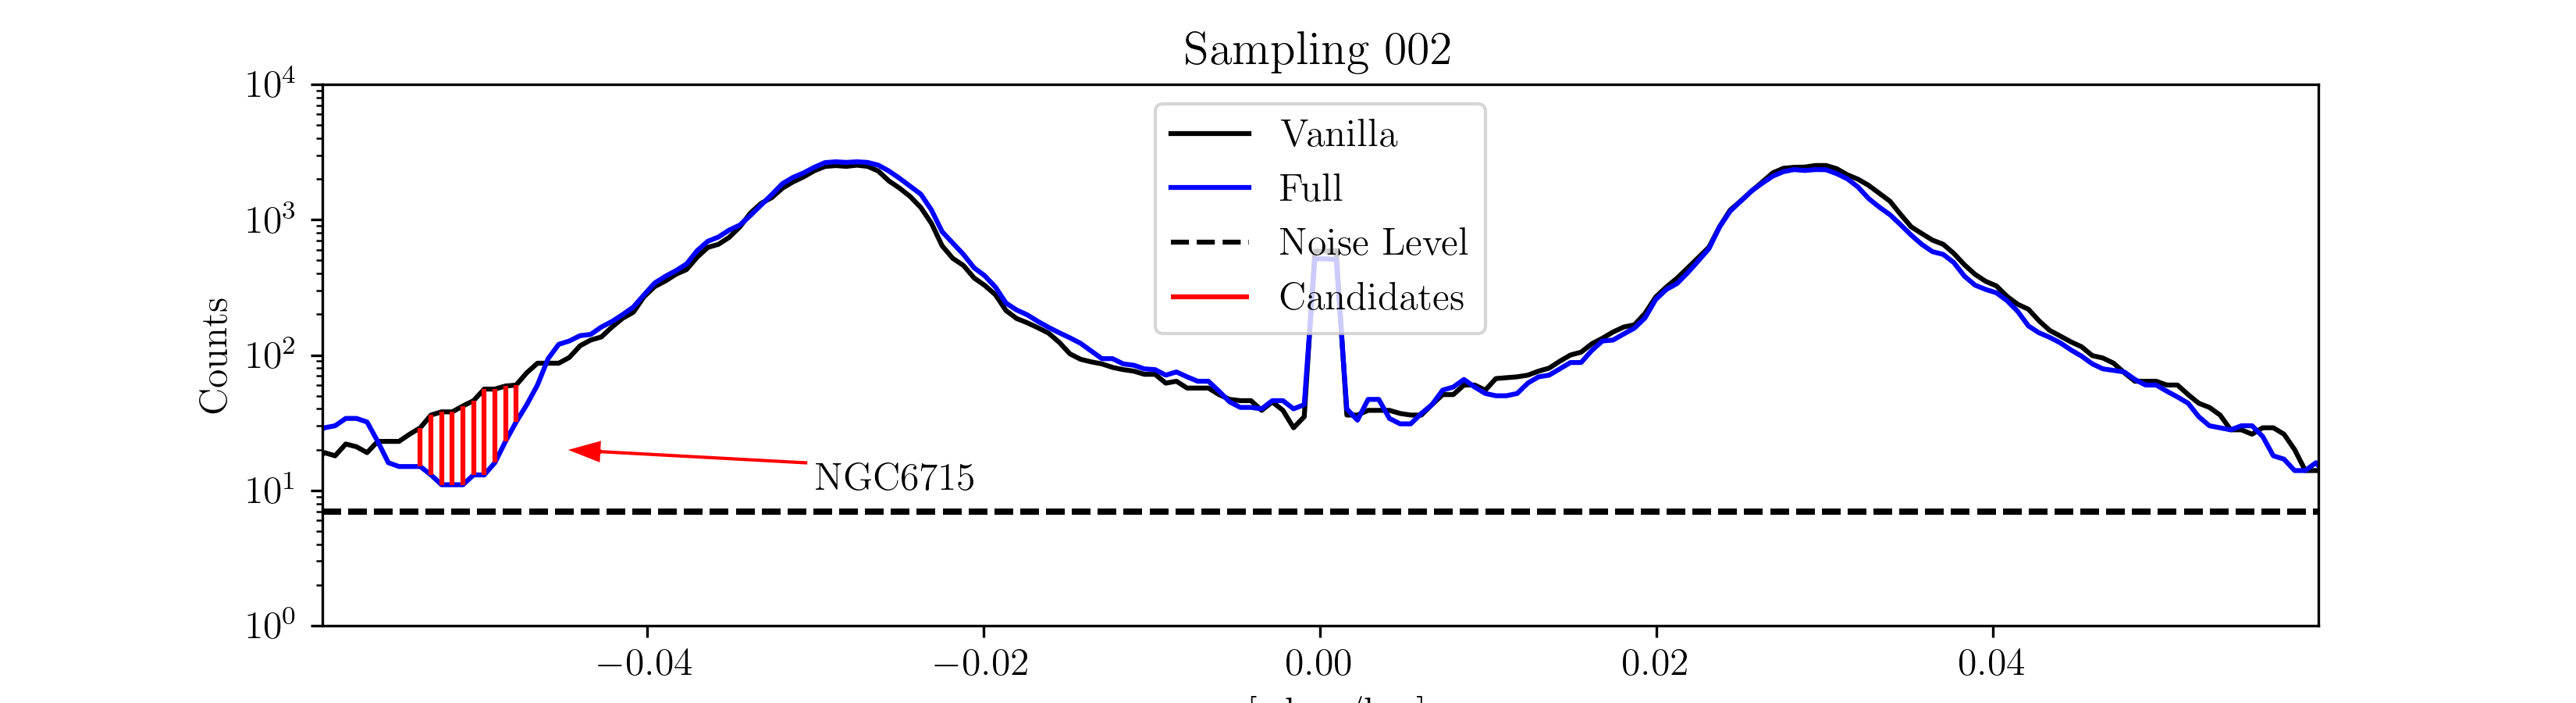
\includegraphics[width=\linewidth]{tau-profile-monte-carlo-002.png}
      \caption{First gap gallery. See the text in Appendix~\ref{sec:gallery_of_gaps} for a description.}
      \label{fig:gallery0}
      \end{figure*}    


    \begin{figure*}
      \centering
      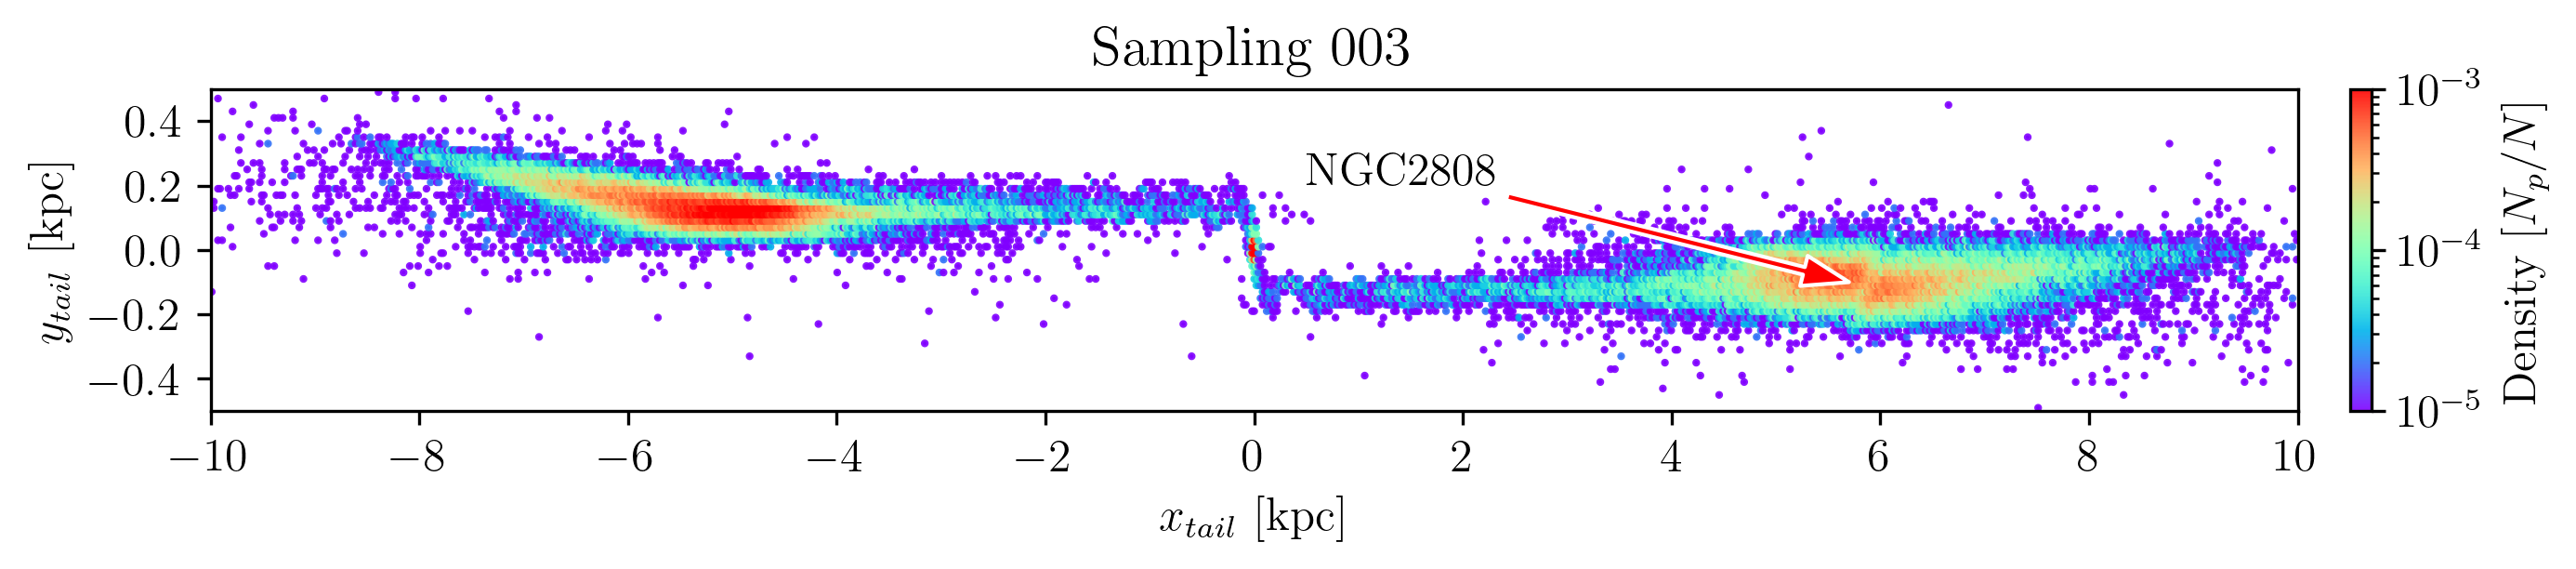
\includegraphics[width=\linewidth]{gallery_of_gaps_monte-carlo-003.png}      
      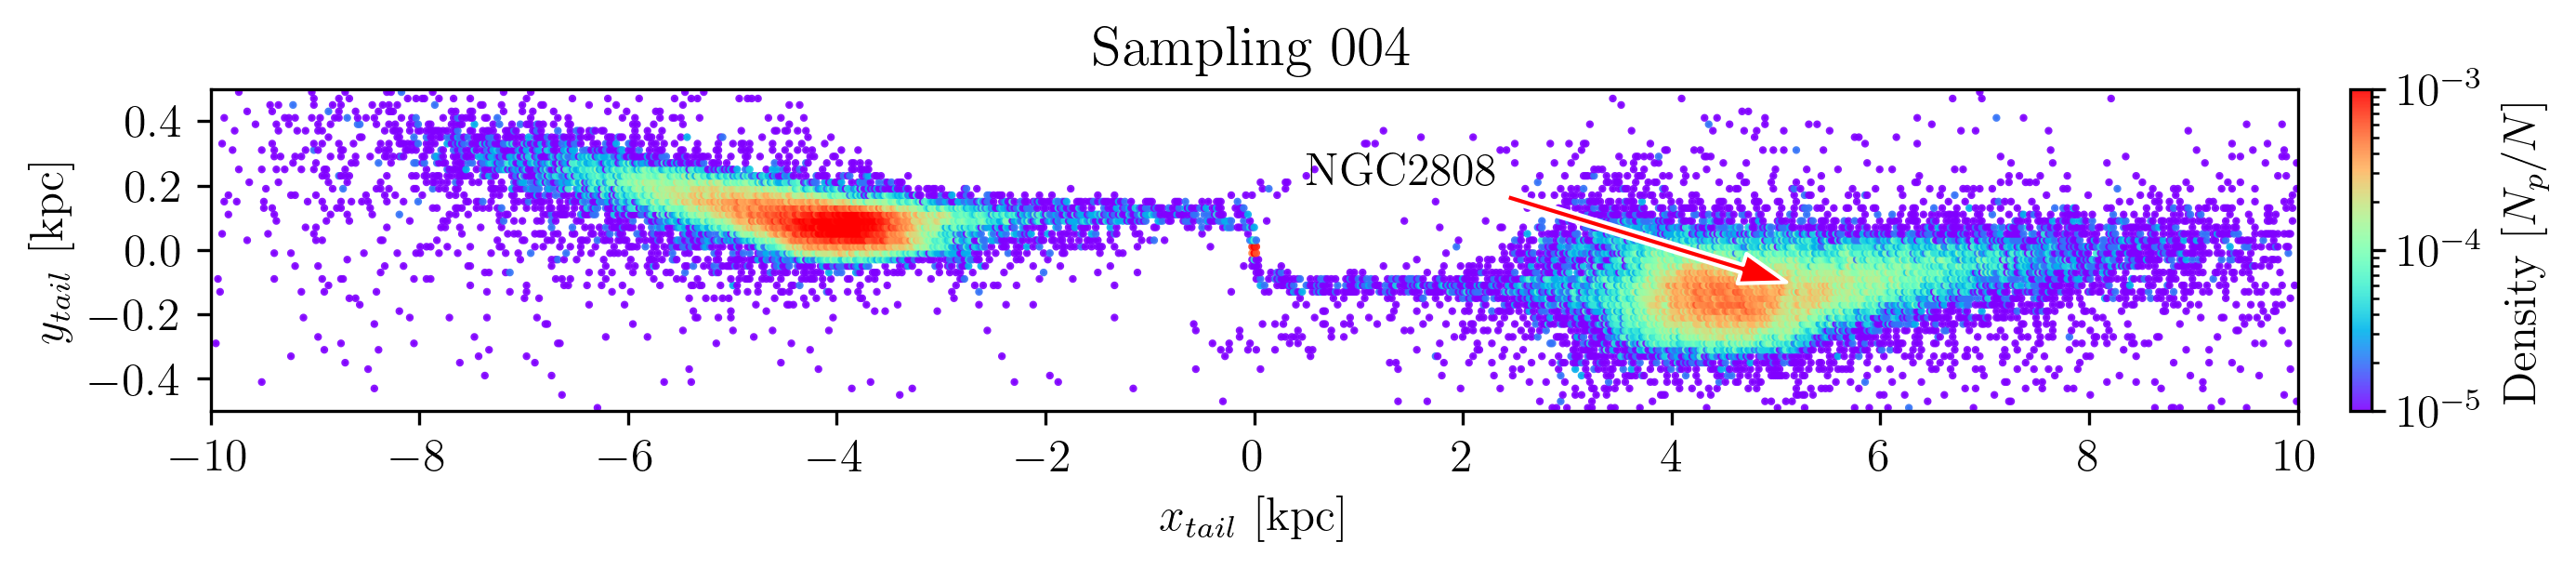
\includegraphics[width=\linewidth]{gallery_of_gaps_monte-carlo-004.png}
      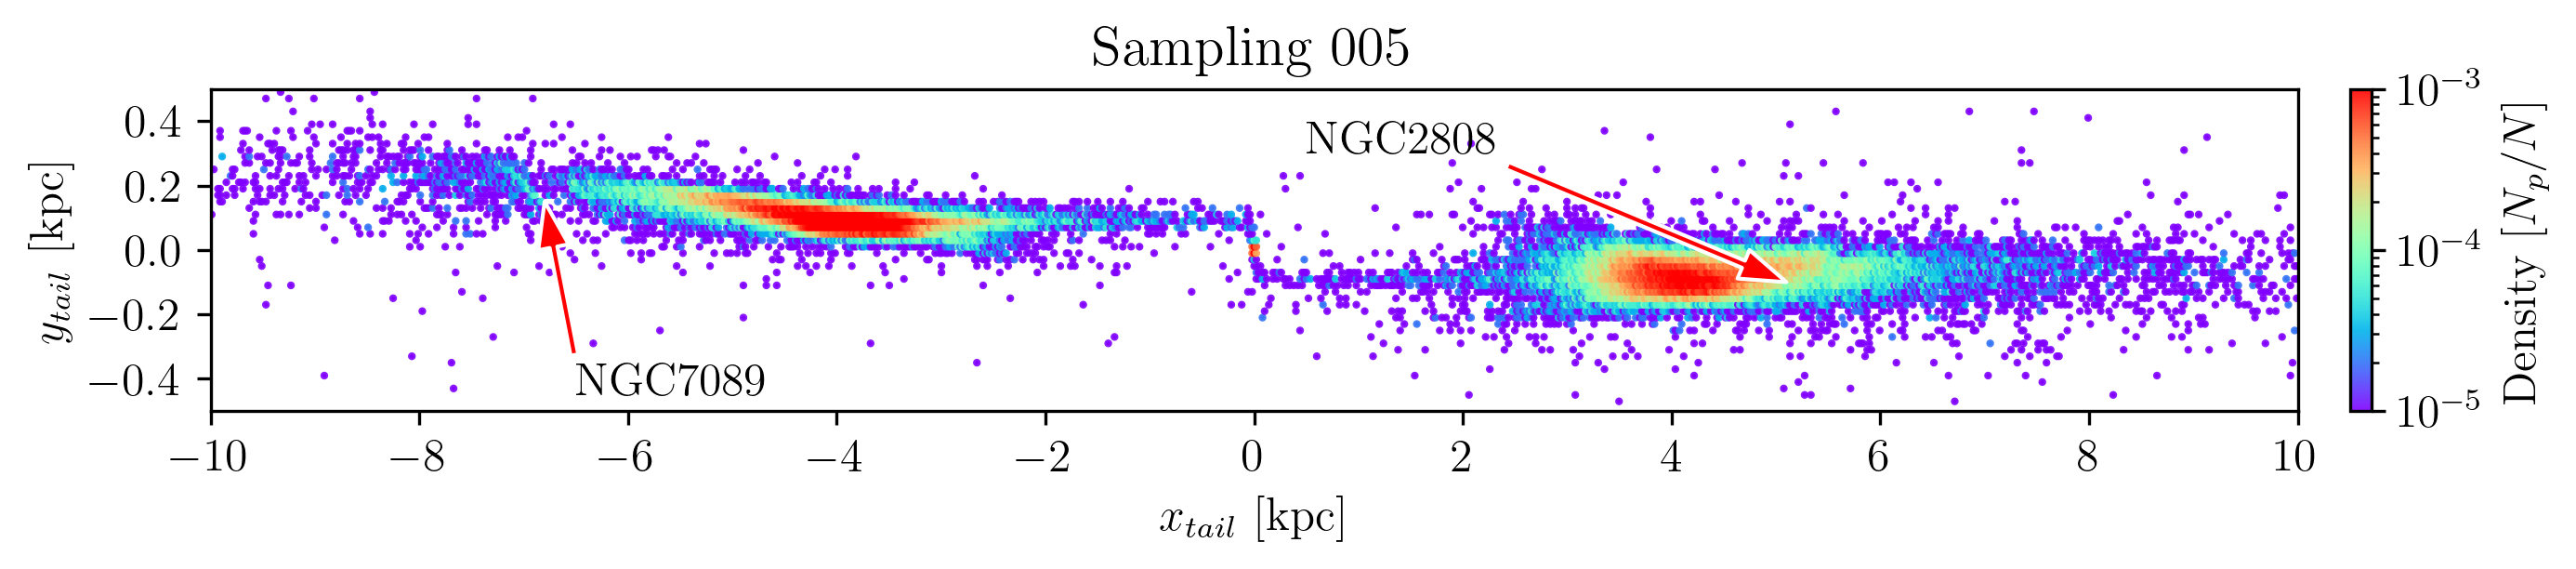
\includegraphics[width=\linewidth]{gallery_of_gaps_monte-carlo-005.png}
      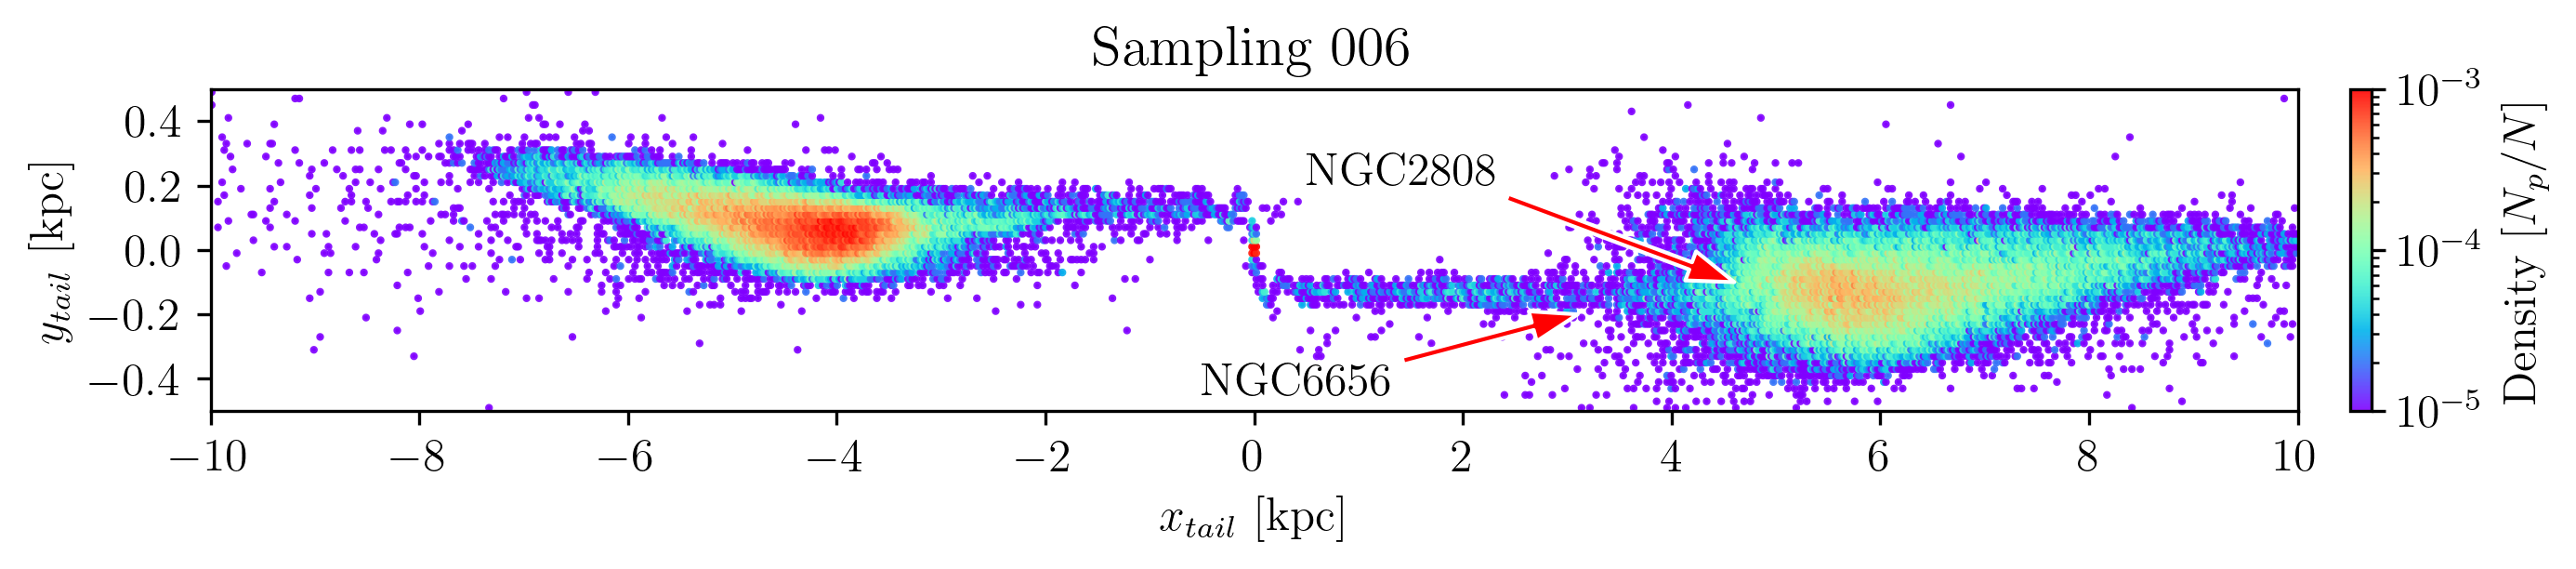
\includegraphics[width=\linewidth]{gallery_of_gaps_monte-carlo-006.png}
      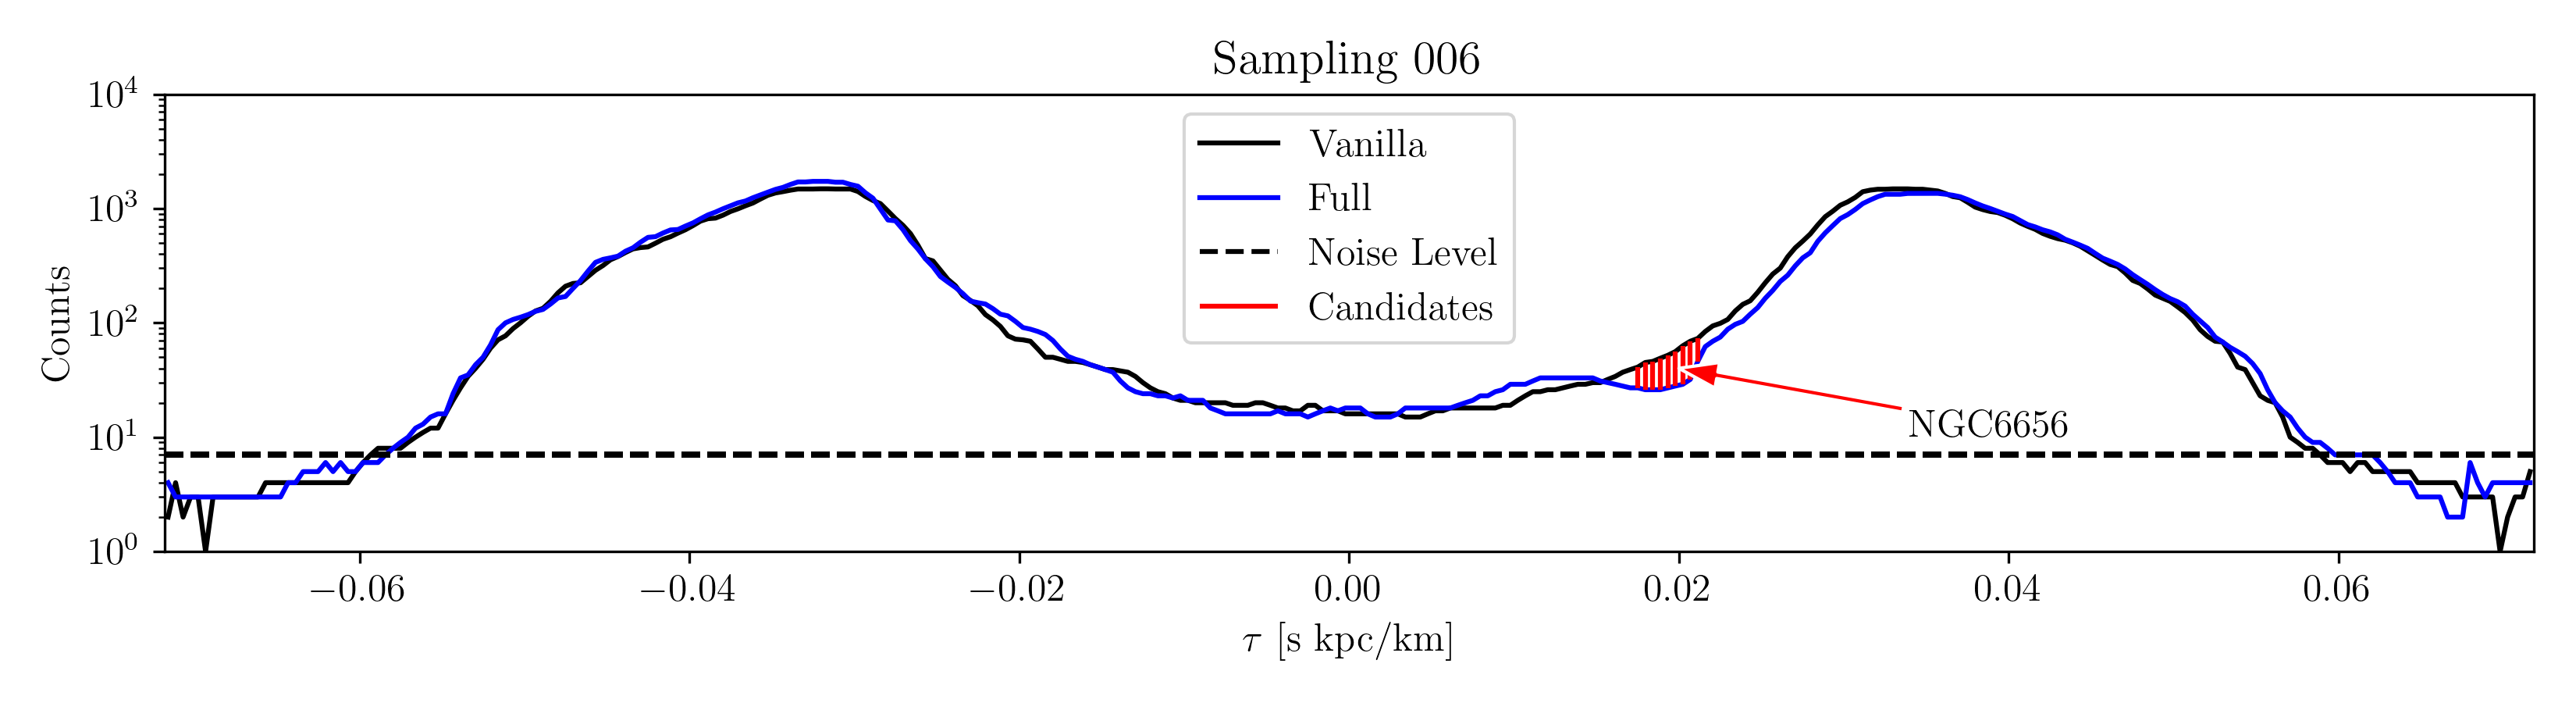
\includegraphics[width=\linewidth]{tau-profile-monte-carlo-006.png}
      \caption{Second gap gallery}
      \label{fig:gallery1}
      \end{figure*}        


    \begin{figure*}
      \centering
      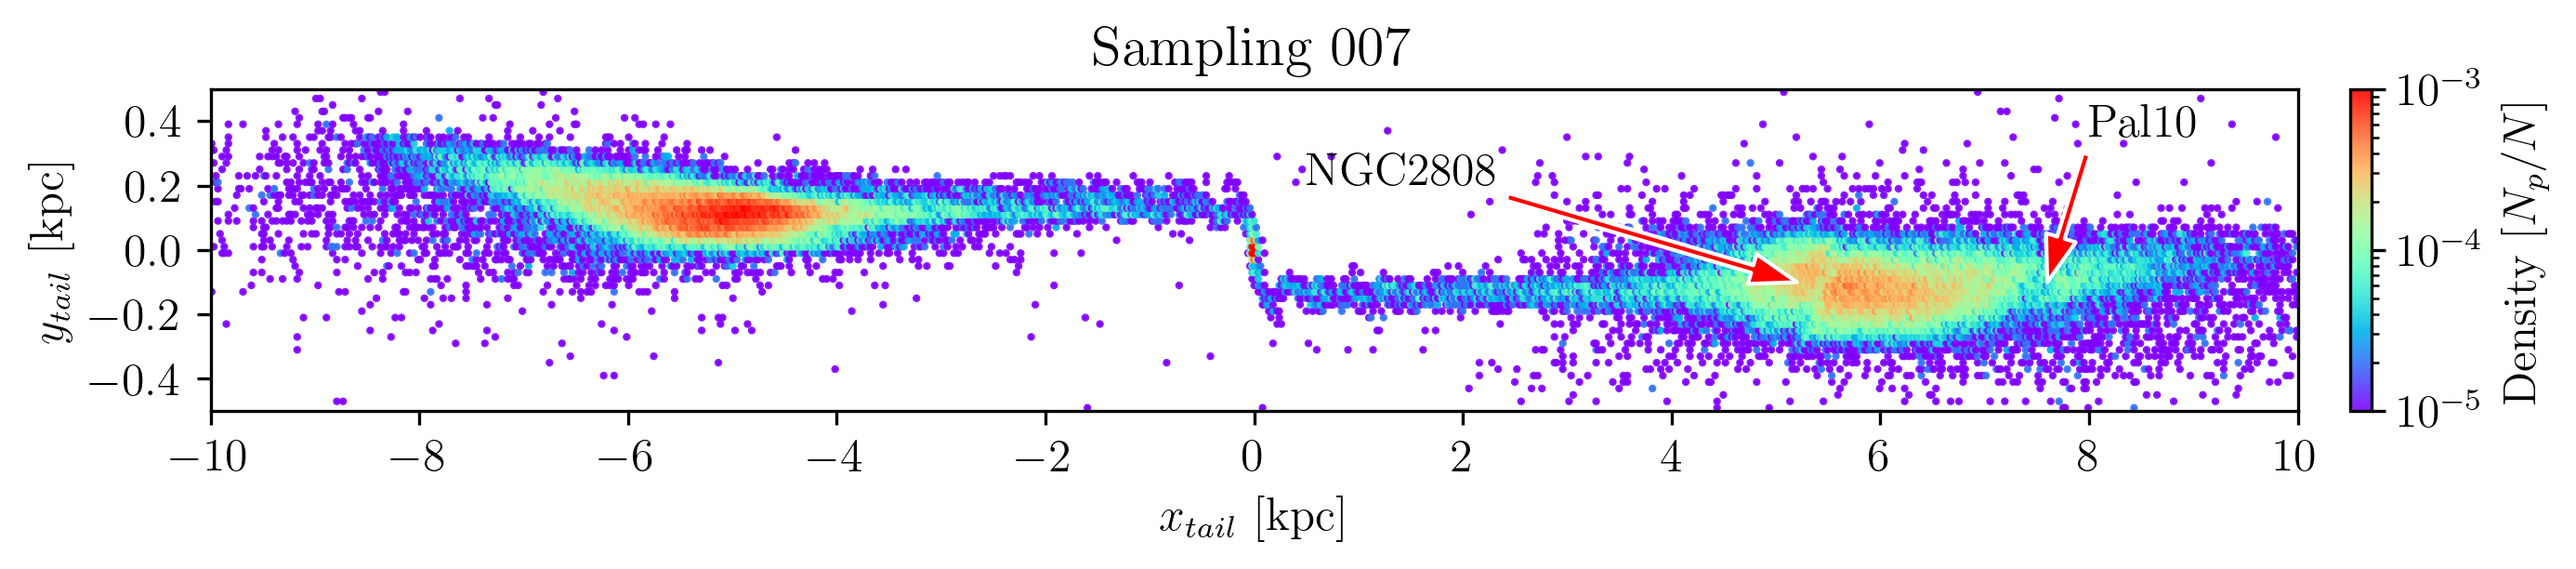
\includegraphics[width=\linewidth]{gallery_of_gaps_monte-carlo-007.png}
      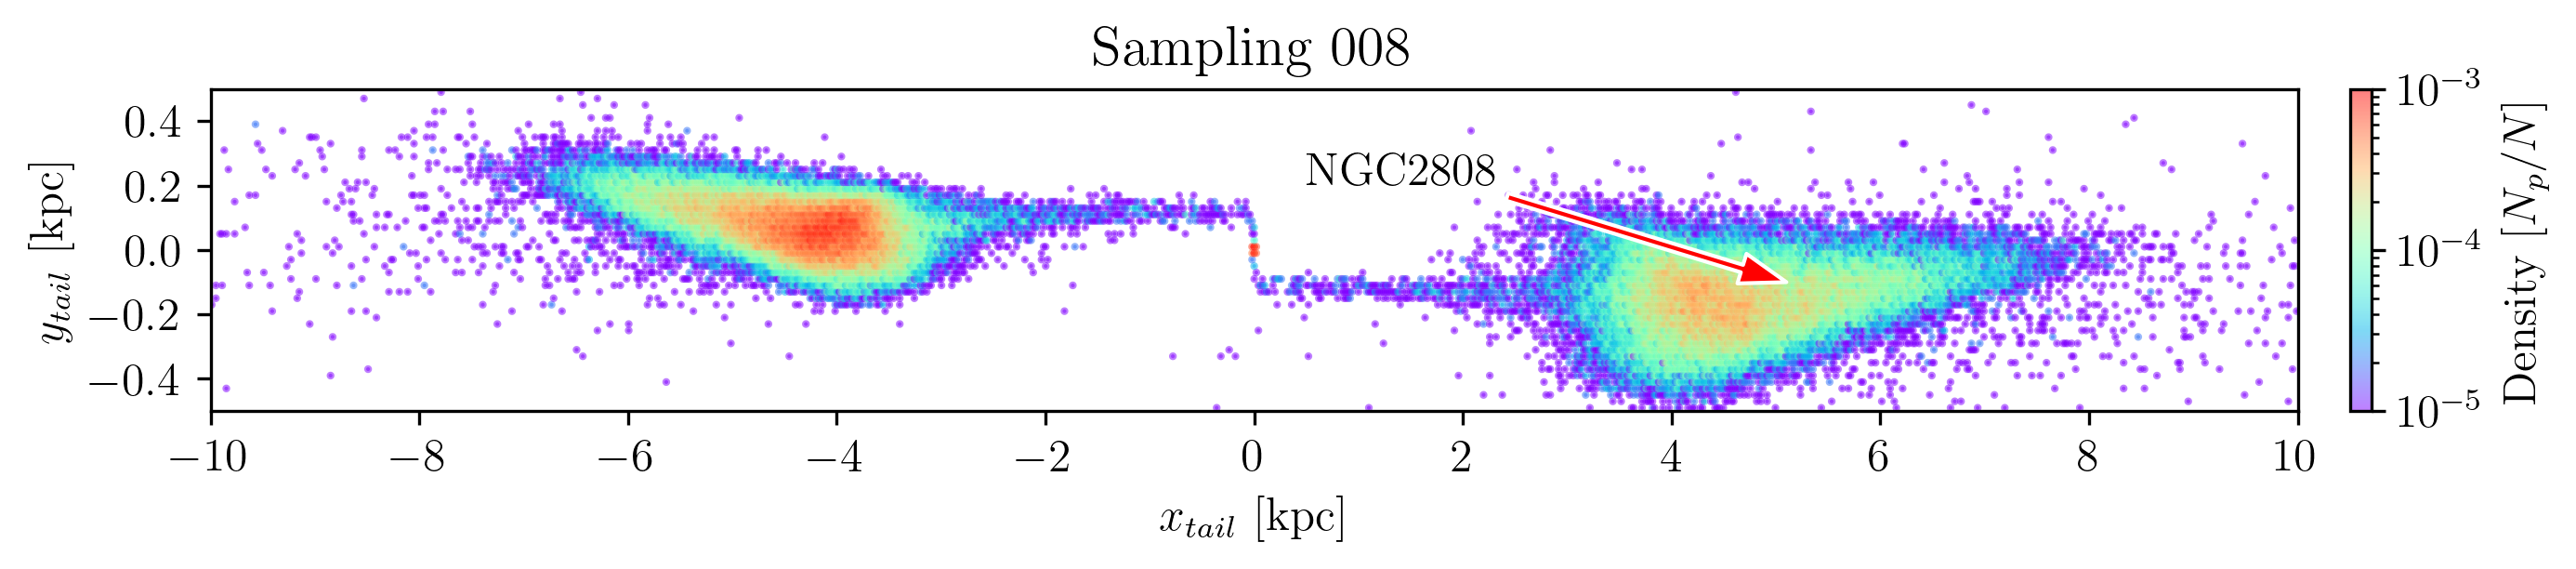
\includegraphics[width=\linewidth]{gallery_of_gaps_monte-carlo-008.png}
      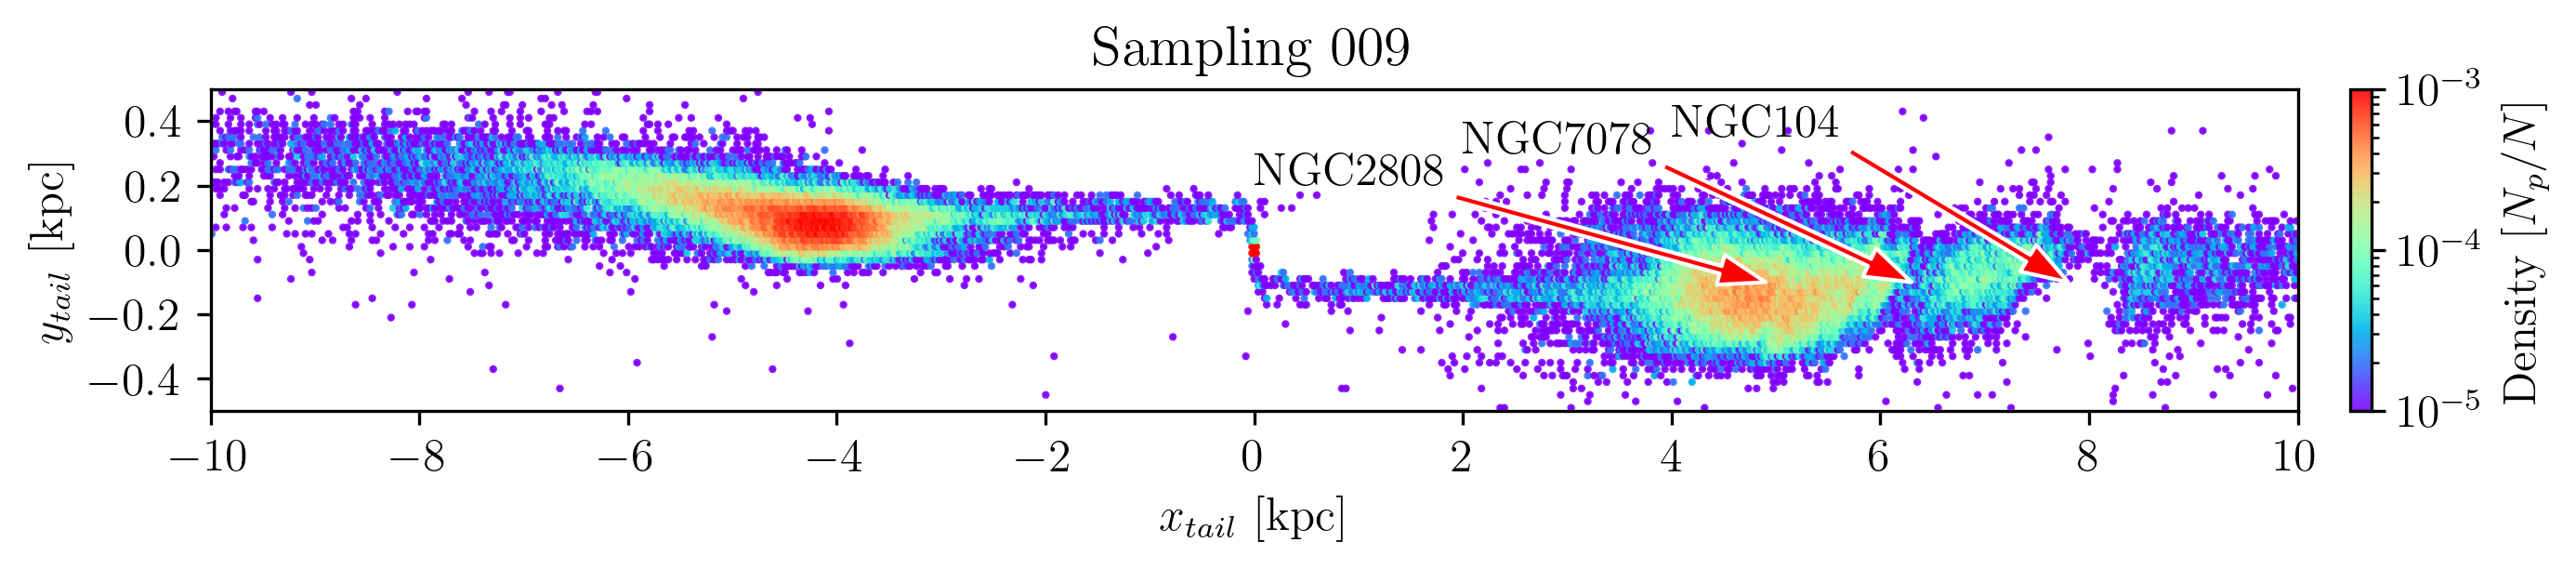
\includegraphics[width=\linewidth]{gallery_of_gaps_monte-carlo-009.png}      
      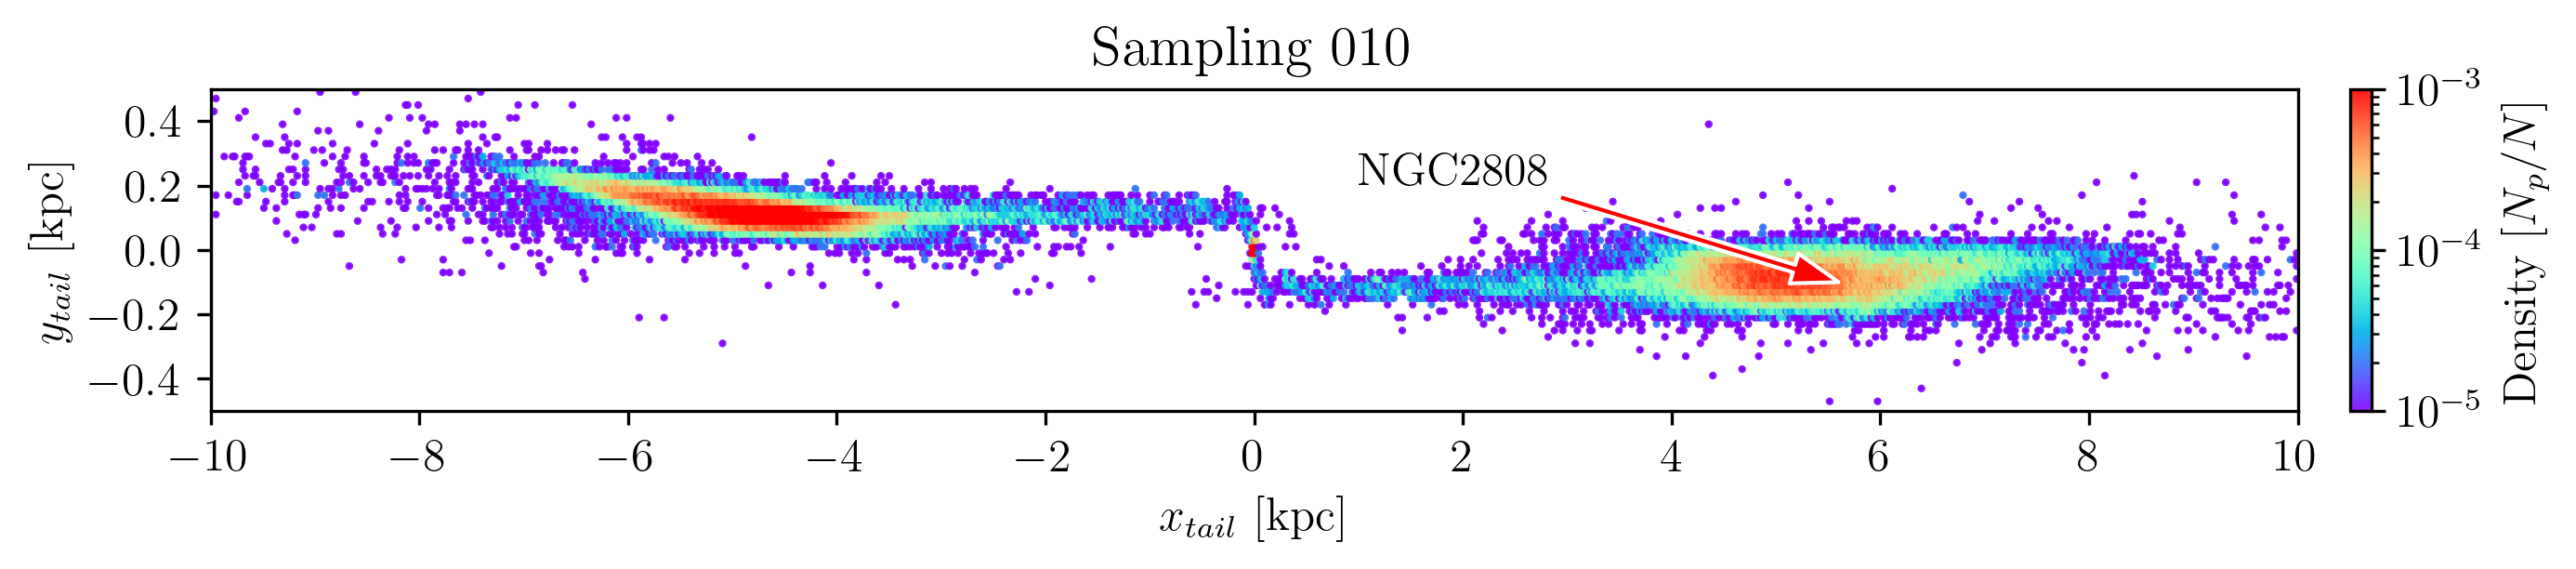
\includegraphics[width=\linewidth]{gallery_of_gaps_monte-carlo-010.png}
      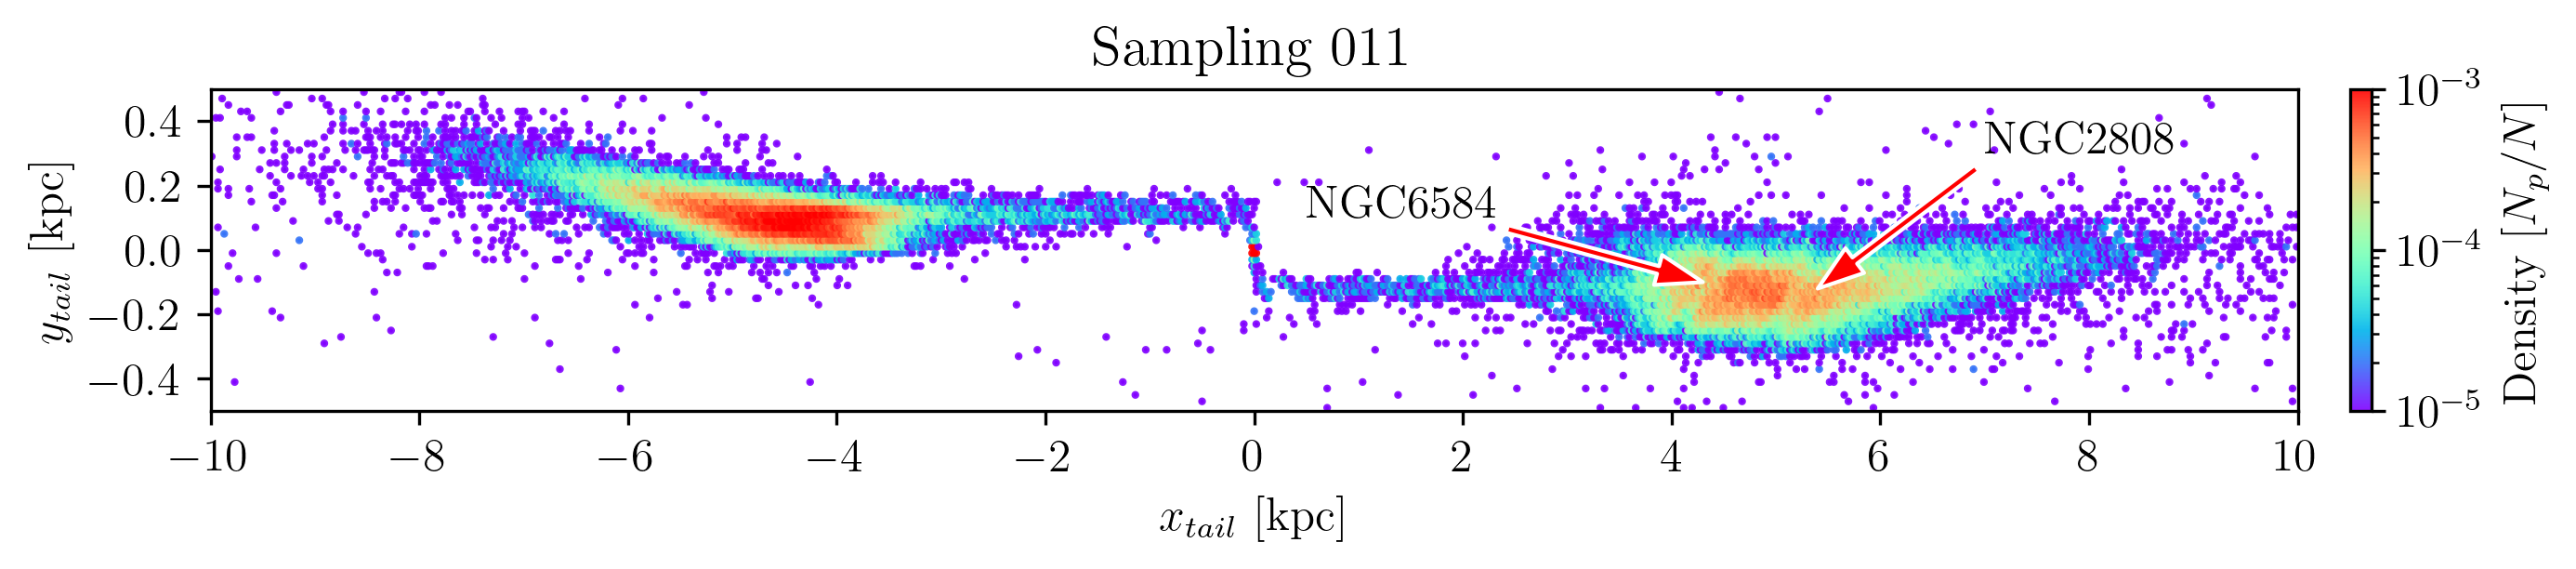
\includegraphics[width=\linewidth]{gallery_of_gaps_monte-carlo-011.png}
      \caption{Third gap gallery}
      \label{fig:gallery2}
      \end{figure*}        


    \begin{figure*}
      \centering
      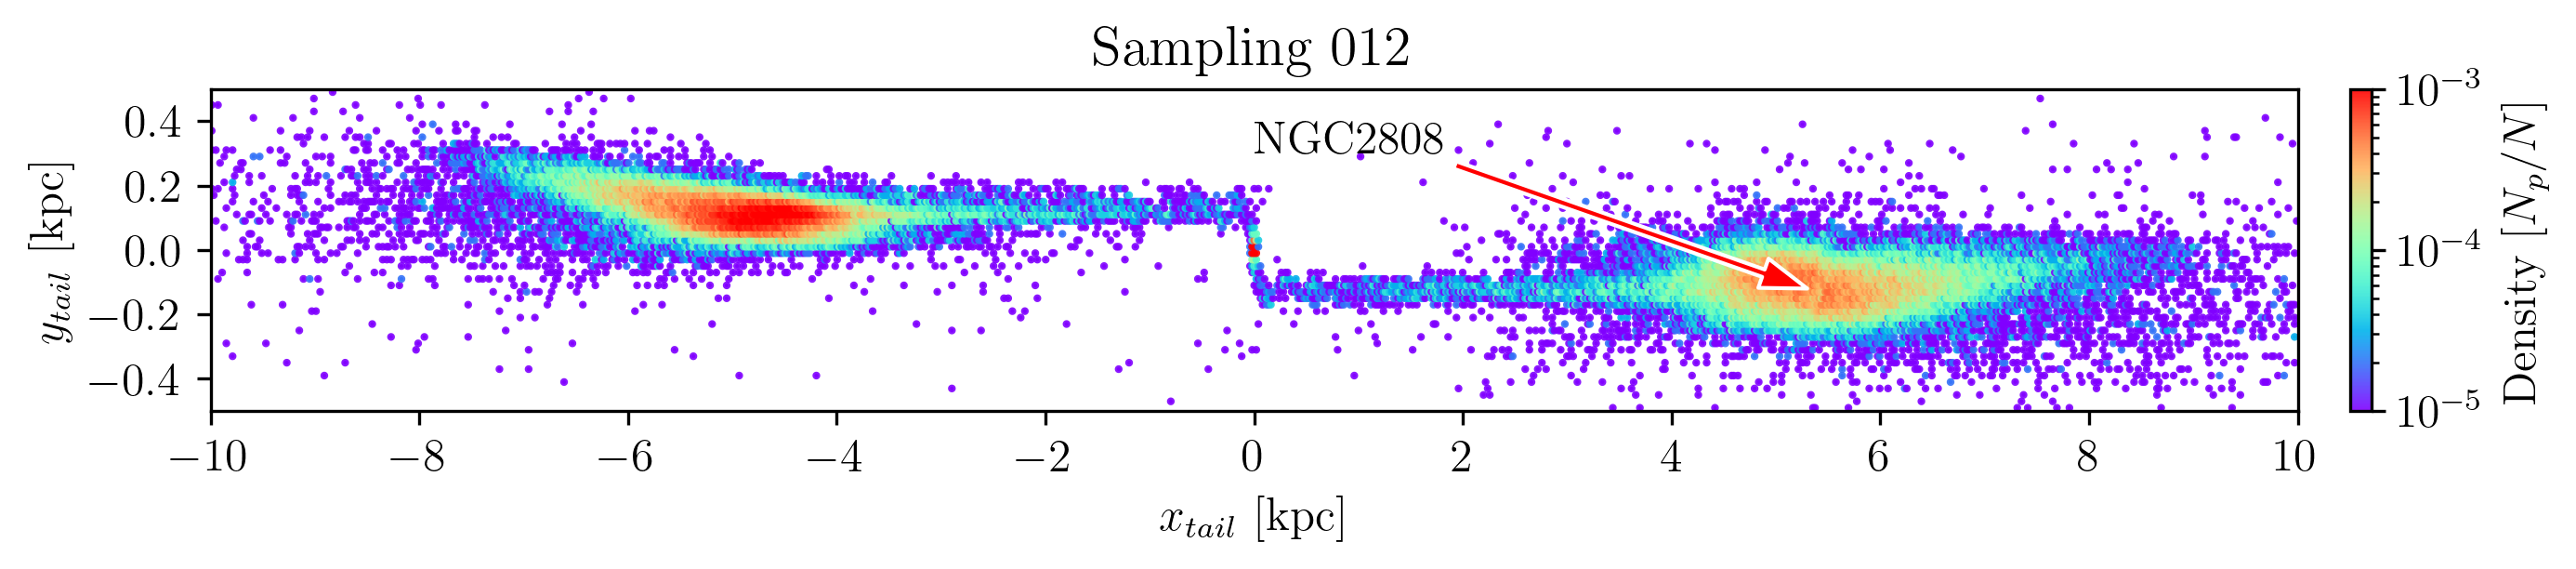
\includegraphics[width=\linewidth]{gallery_of_gaps_monte-carlo-012.png}
      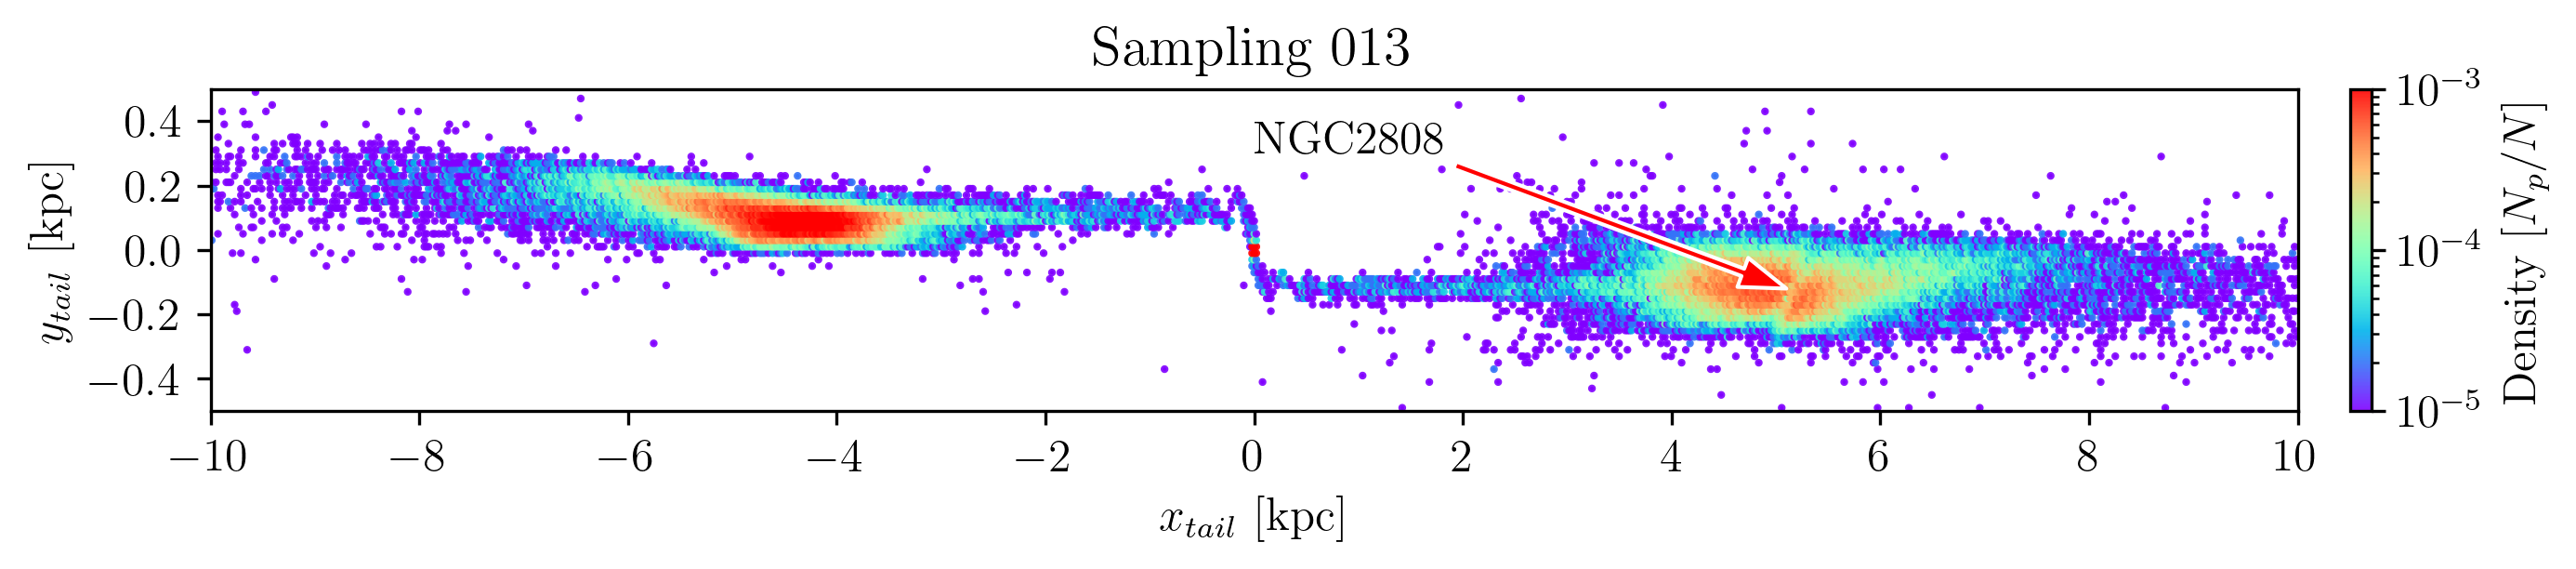
\includegraphics[width=\linewidth]{gallery_of_gaps_monte-carlo-013.png}
      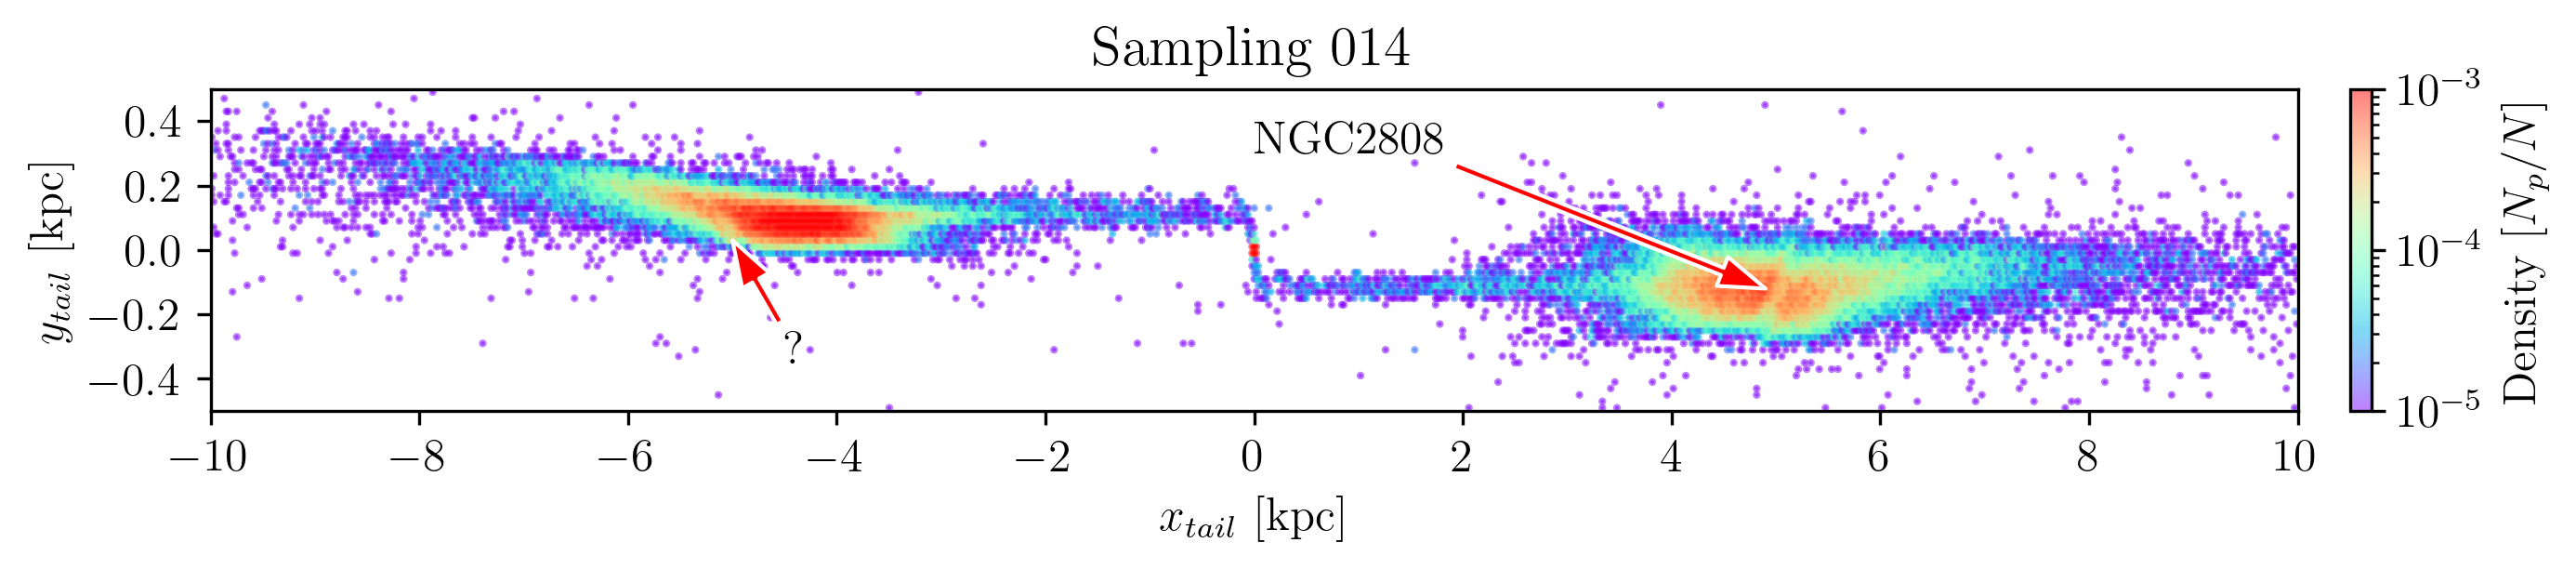
\includegraphics[width=\linewidth]{gallery_of_gaps_monte-carlo-014.png}      
      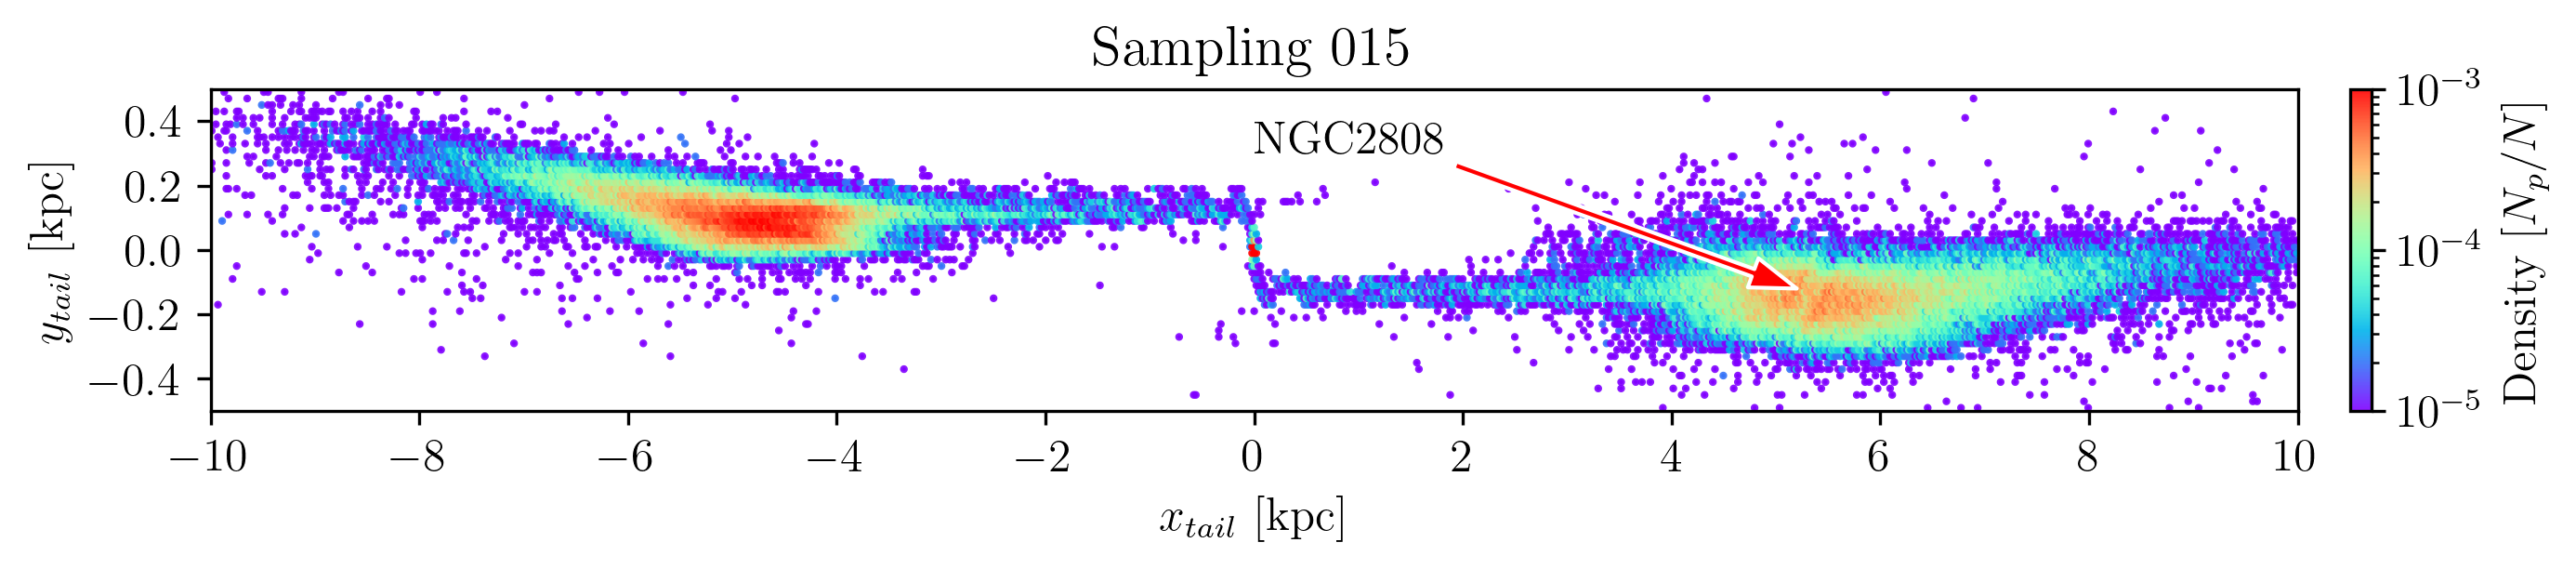
\includegraphics[width=\linewidth]{gallery_of_gaps_monte-carlo-015.png}
      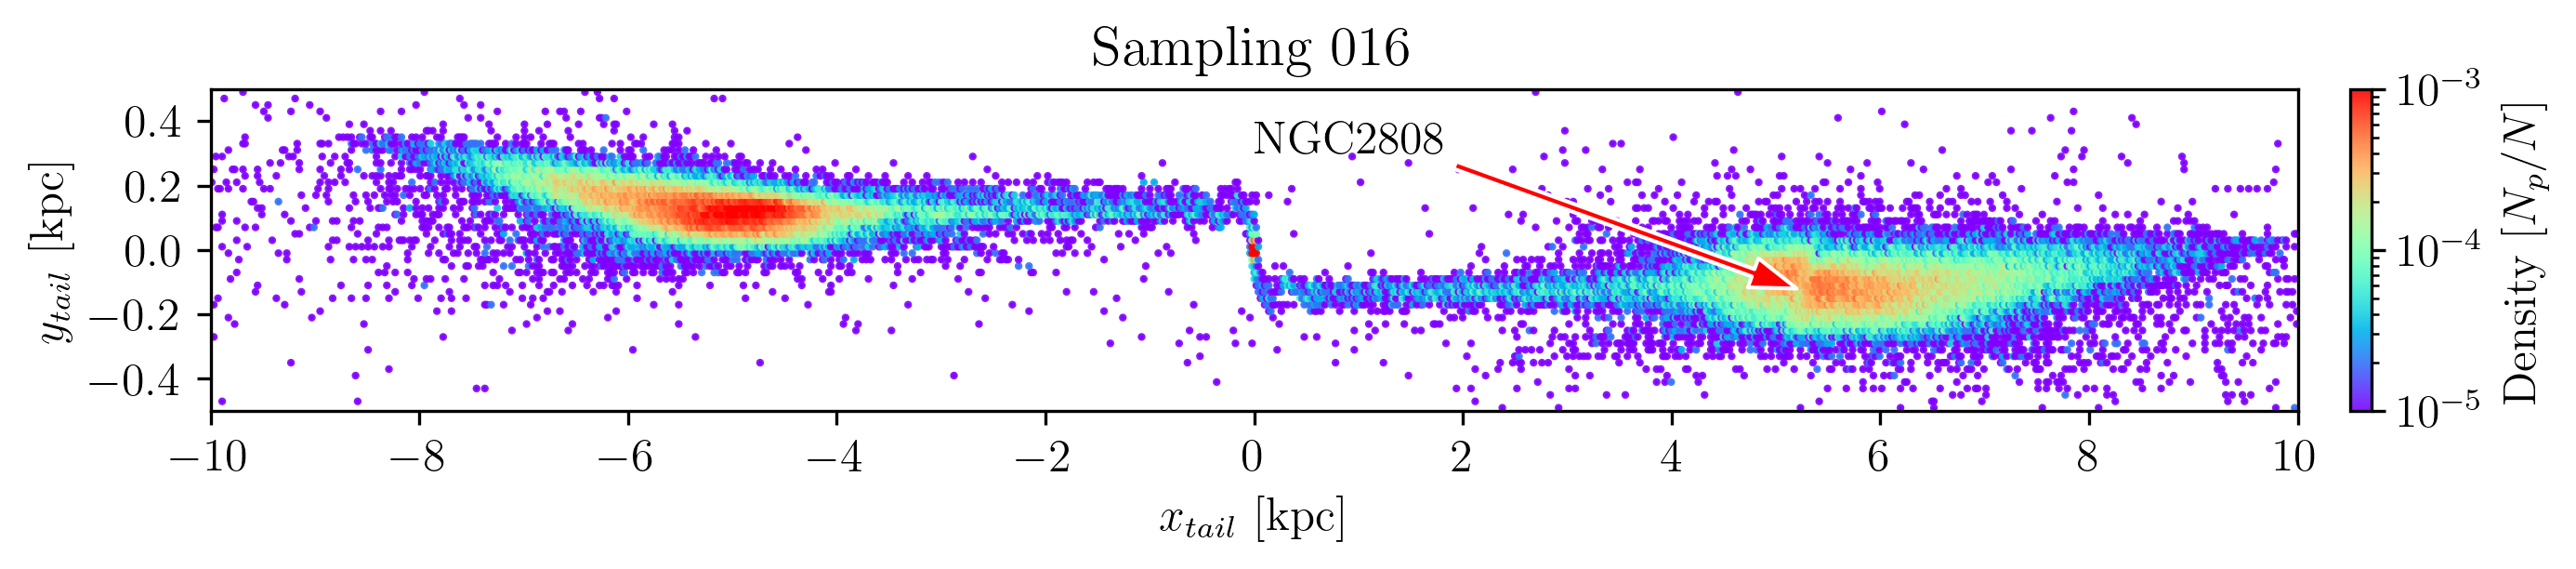
\includegraphics[width=\linewidth]{gallery_of_gaps_monte-carlo-016.png}
      \caption{Fourth gap gallery}
      \label{fig:gallery3}
      \end{figure*}        

    \begin{figure*}
      \centering
      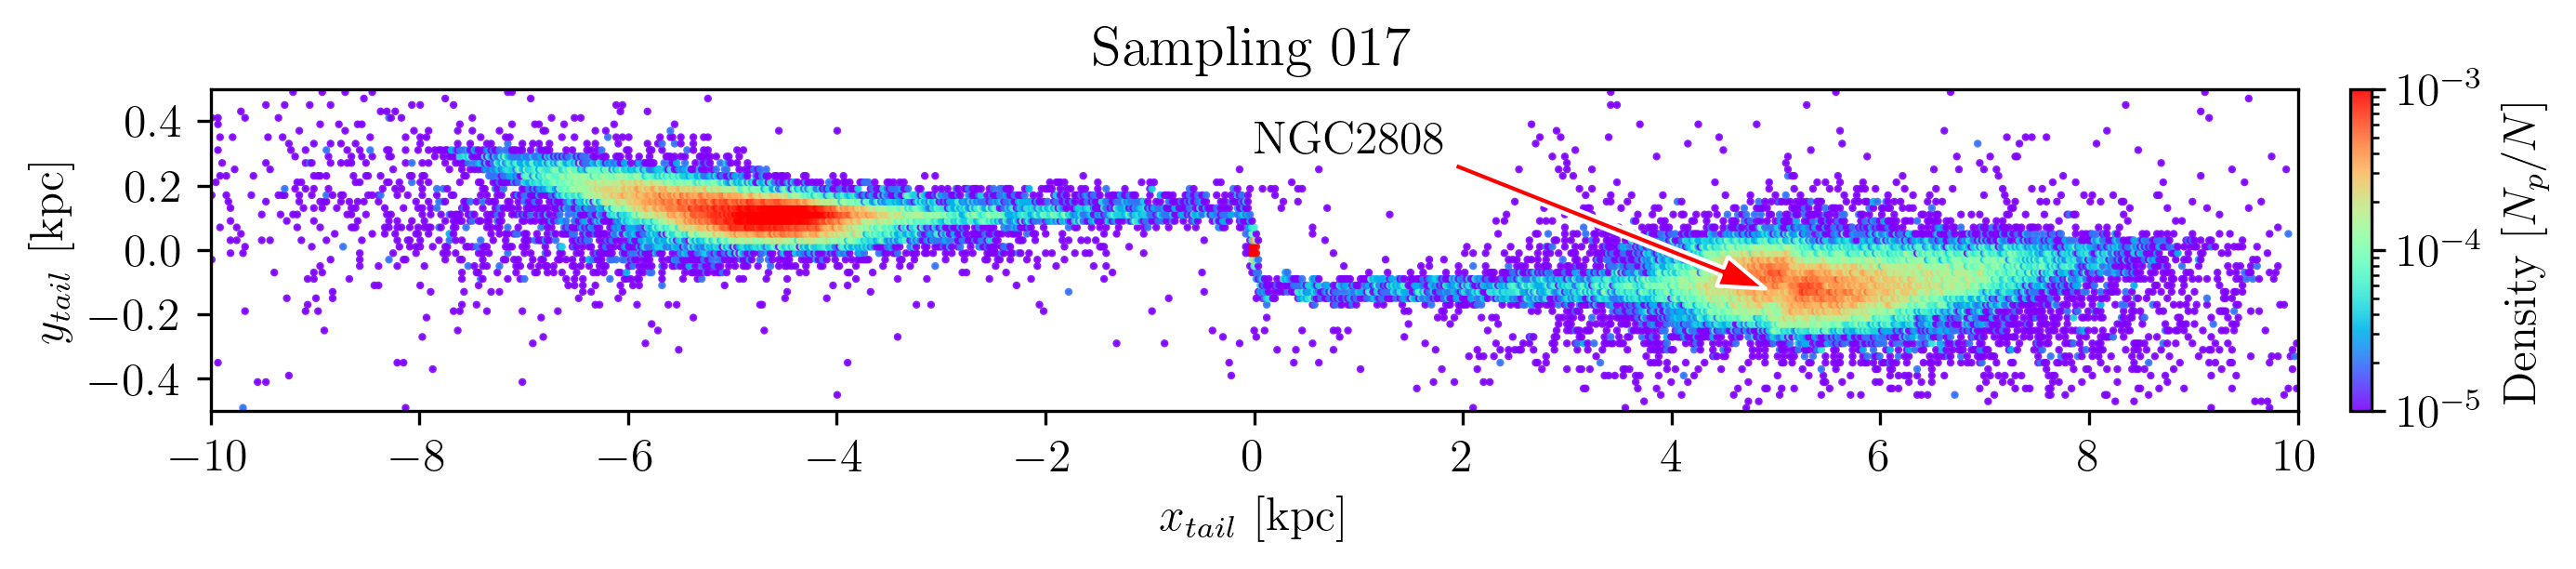
\includegraphics[width=\linewidth]{gallery_of_gaps_monte-carlo-017.png}
      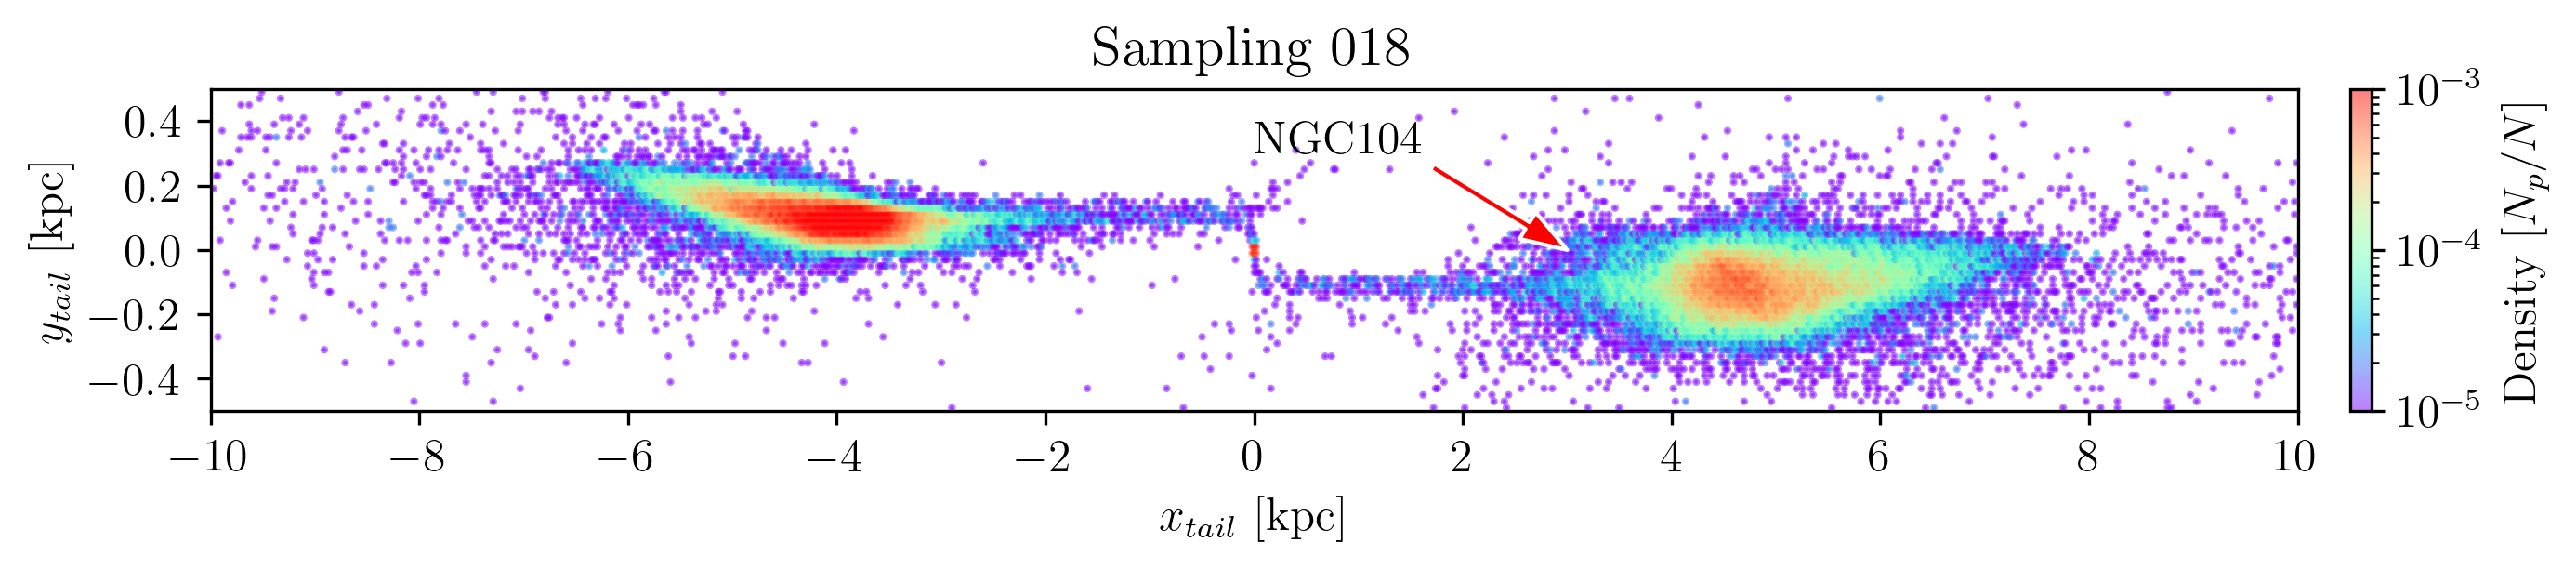
\includegraphics[width=\linewidth]{gallery_of_gaps_monte-carlo-018.png}
      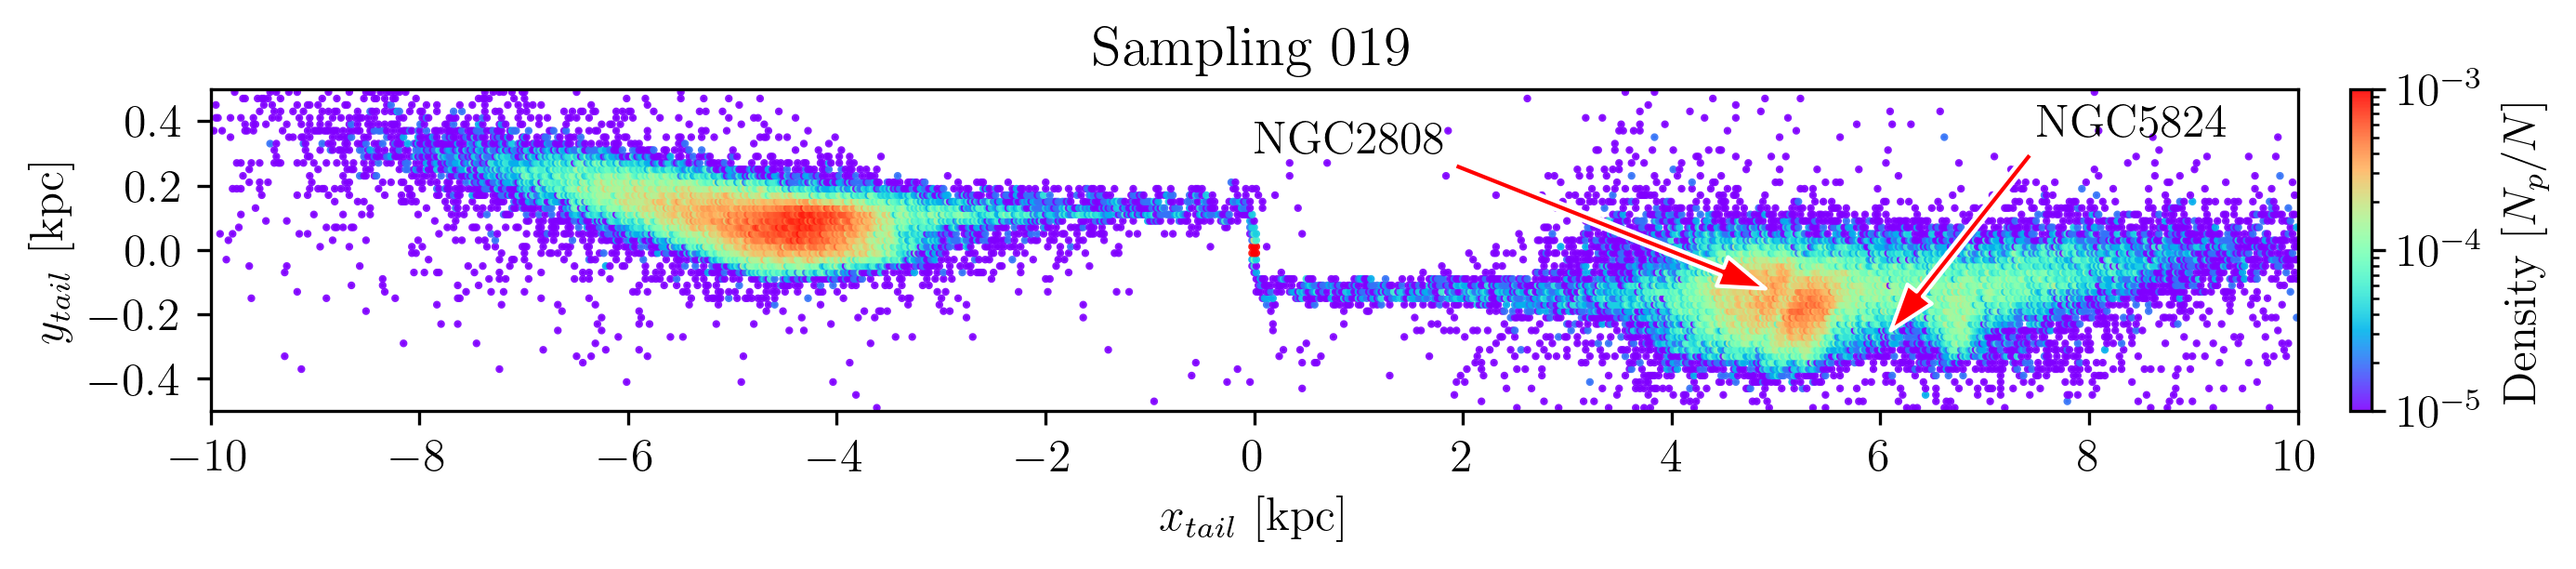
\includegraphics[width=\linewidth]{gallery_of_gaps_monte-carlo-019.png}      
      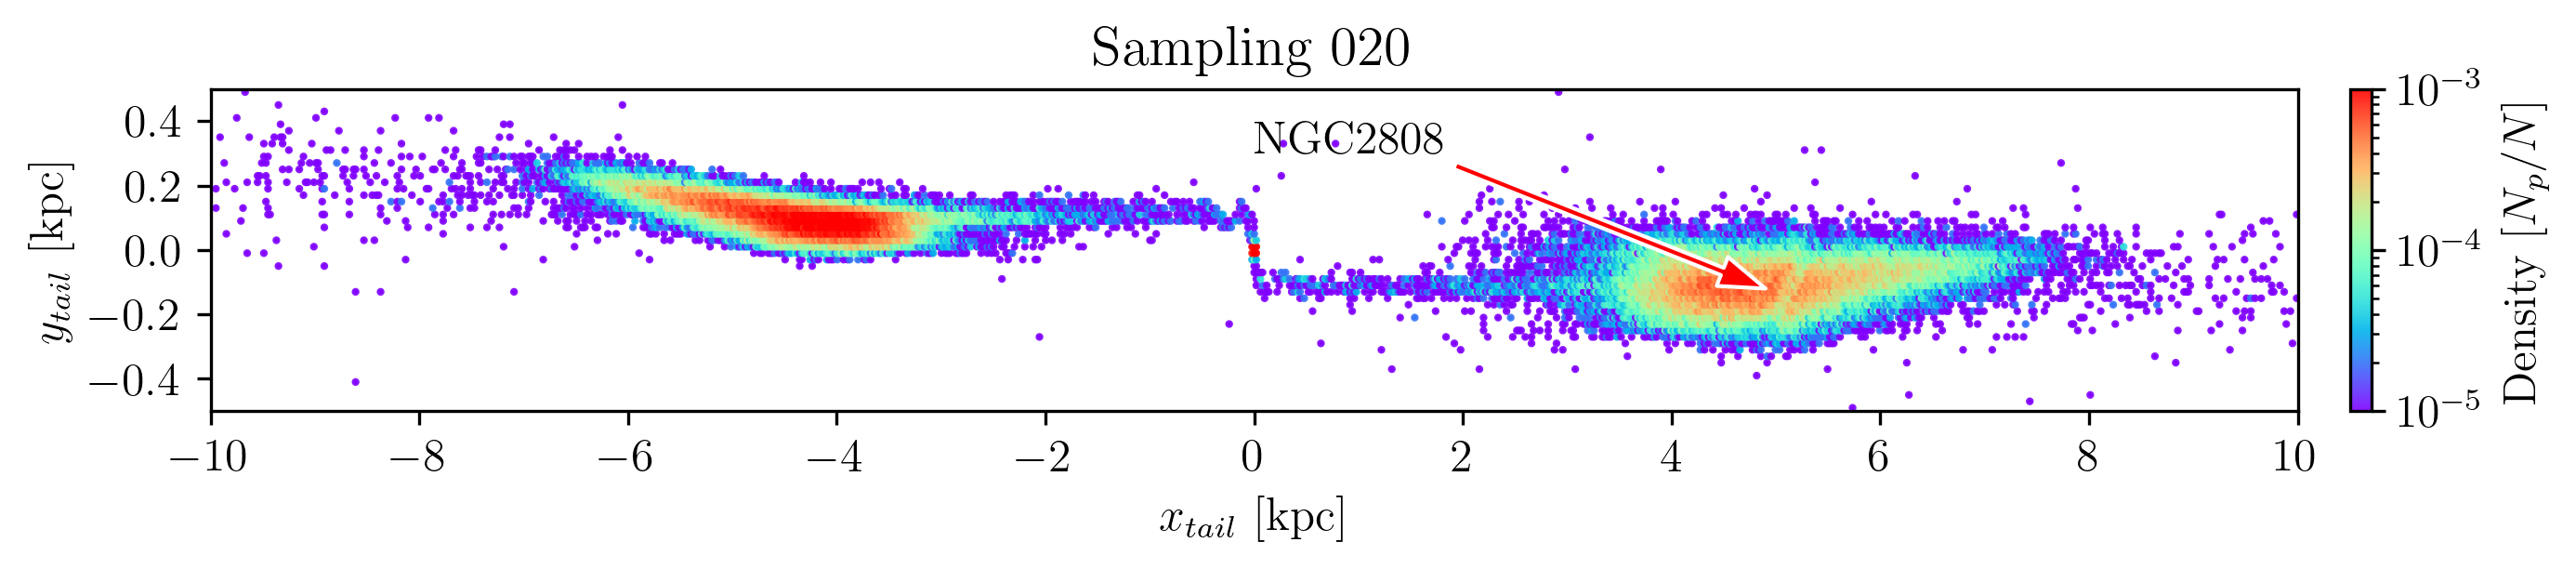
\includegraphics[width=\linewidth]{gallery_of_gaps_monte-carlo-020.png}
      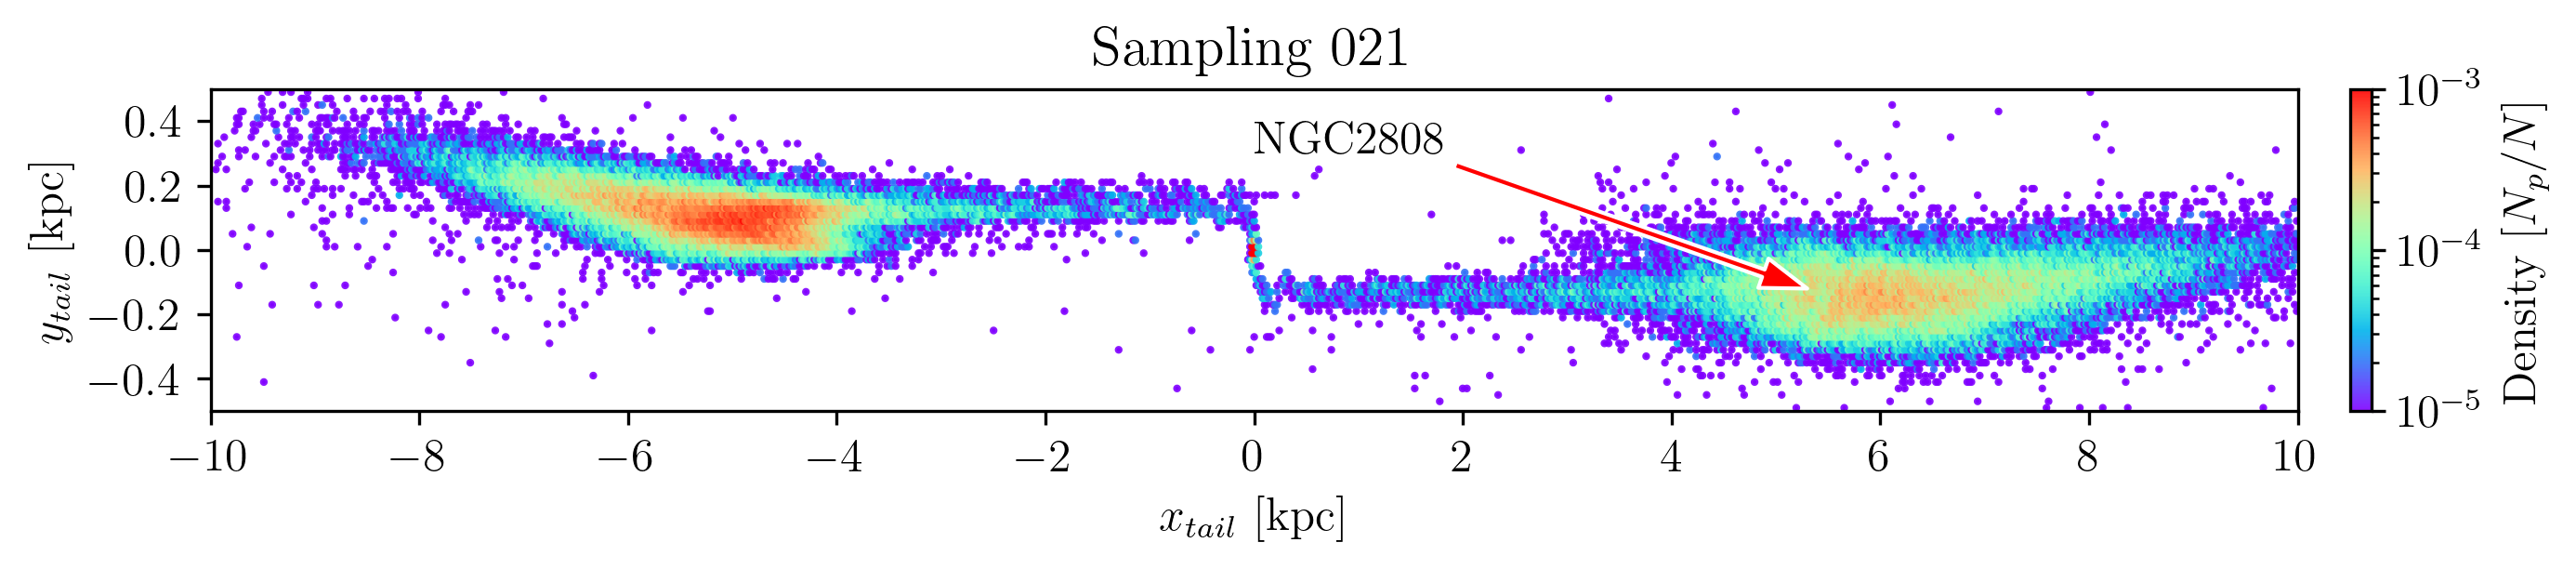
\includegraphics[width=\linewidth]{gallery_of_gaps_monte-carlo-021.png}
      \caption{Fifth gap gallery}
      \label{fig:gallery4}
      \end{figure*}        

    \begin{figure*}
      \centering
      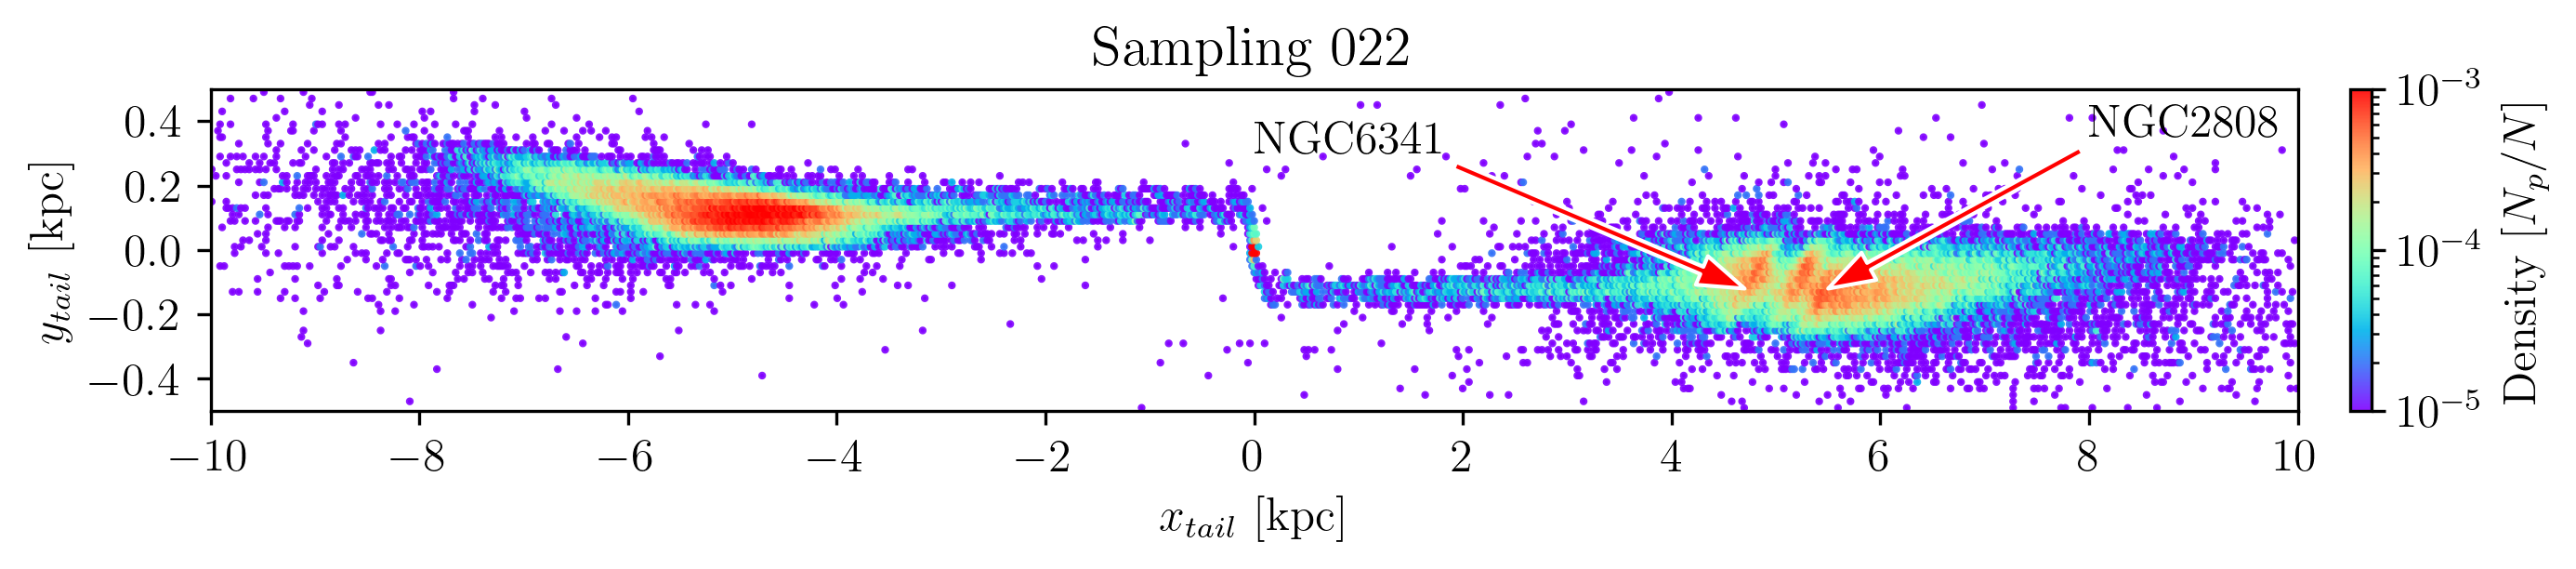
\includegraphics[width=\linewidth]{gallery_of_gaps_monte-carlo-022.png}
      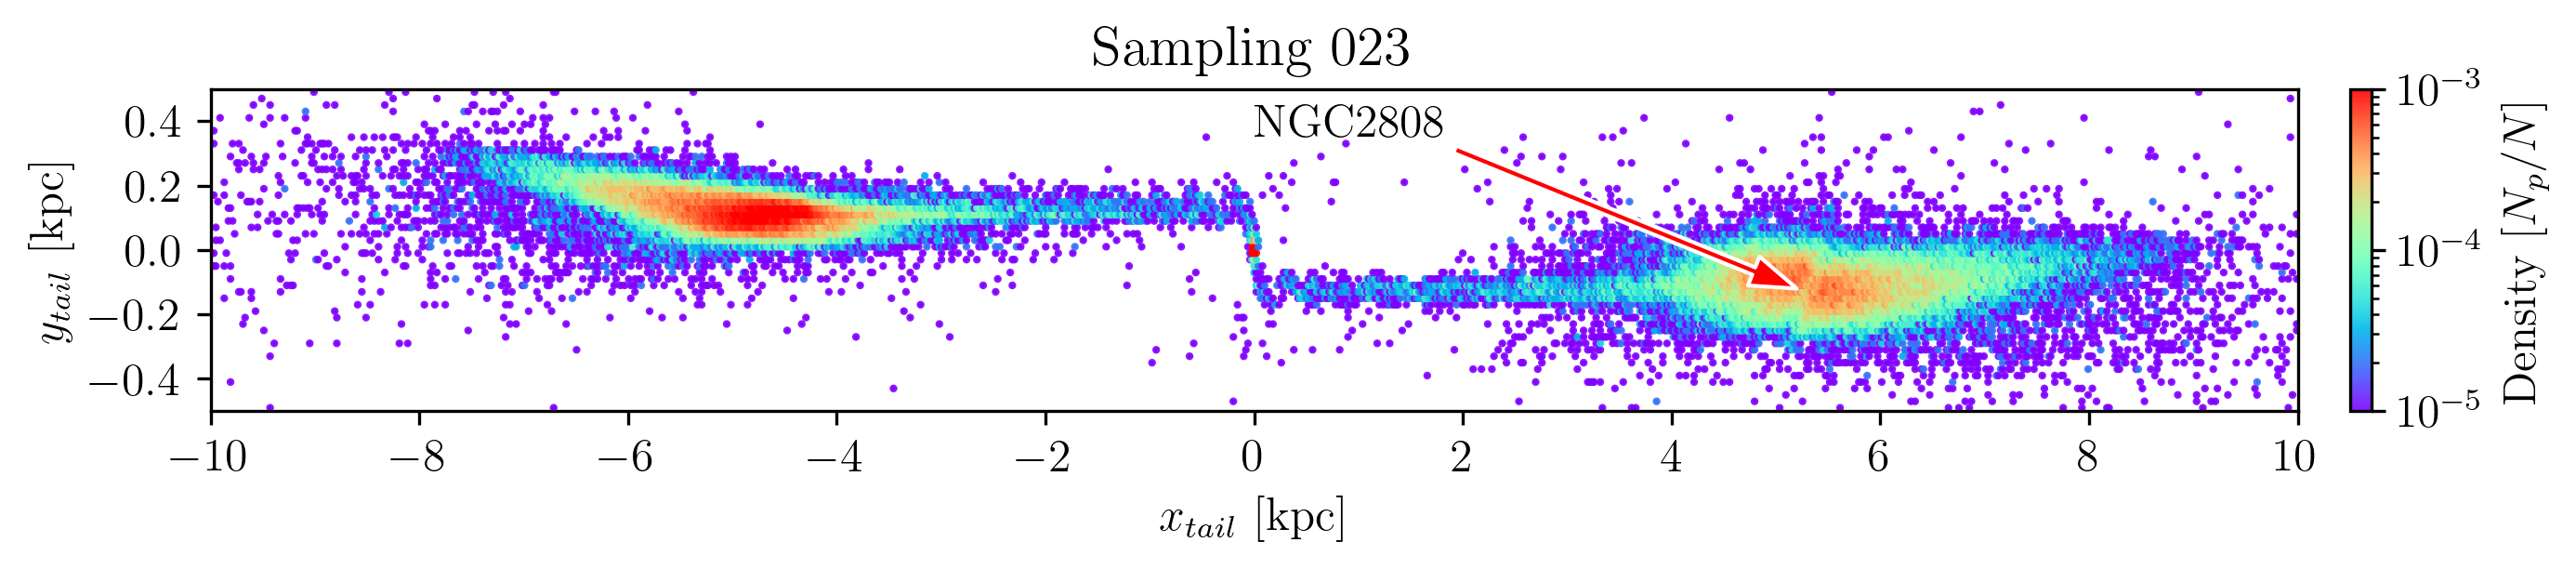
\includegraphics[width=\linewidth]{gallery_of_gaps_monte-carlo-023.png}
      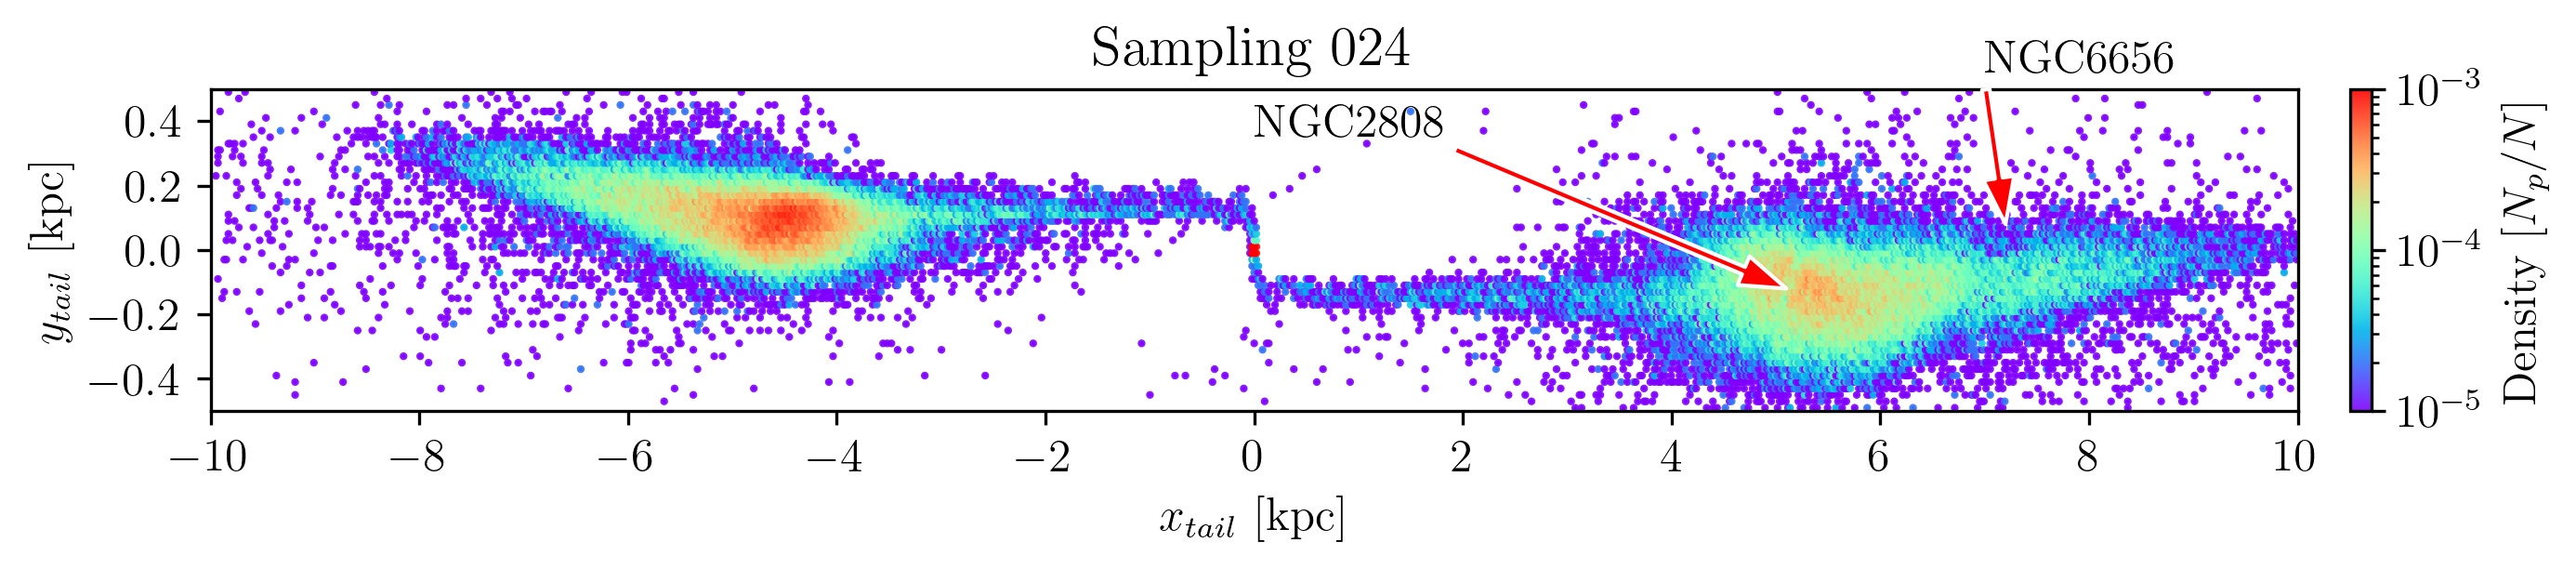
\includegraphics[width=\linewidth]{gallery_of_gaps_monte-carlo-024.png}   
      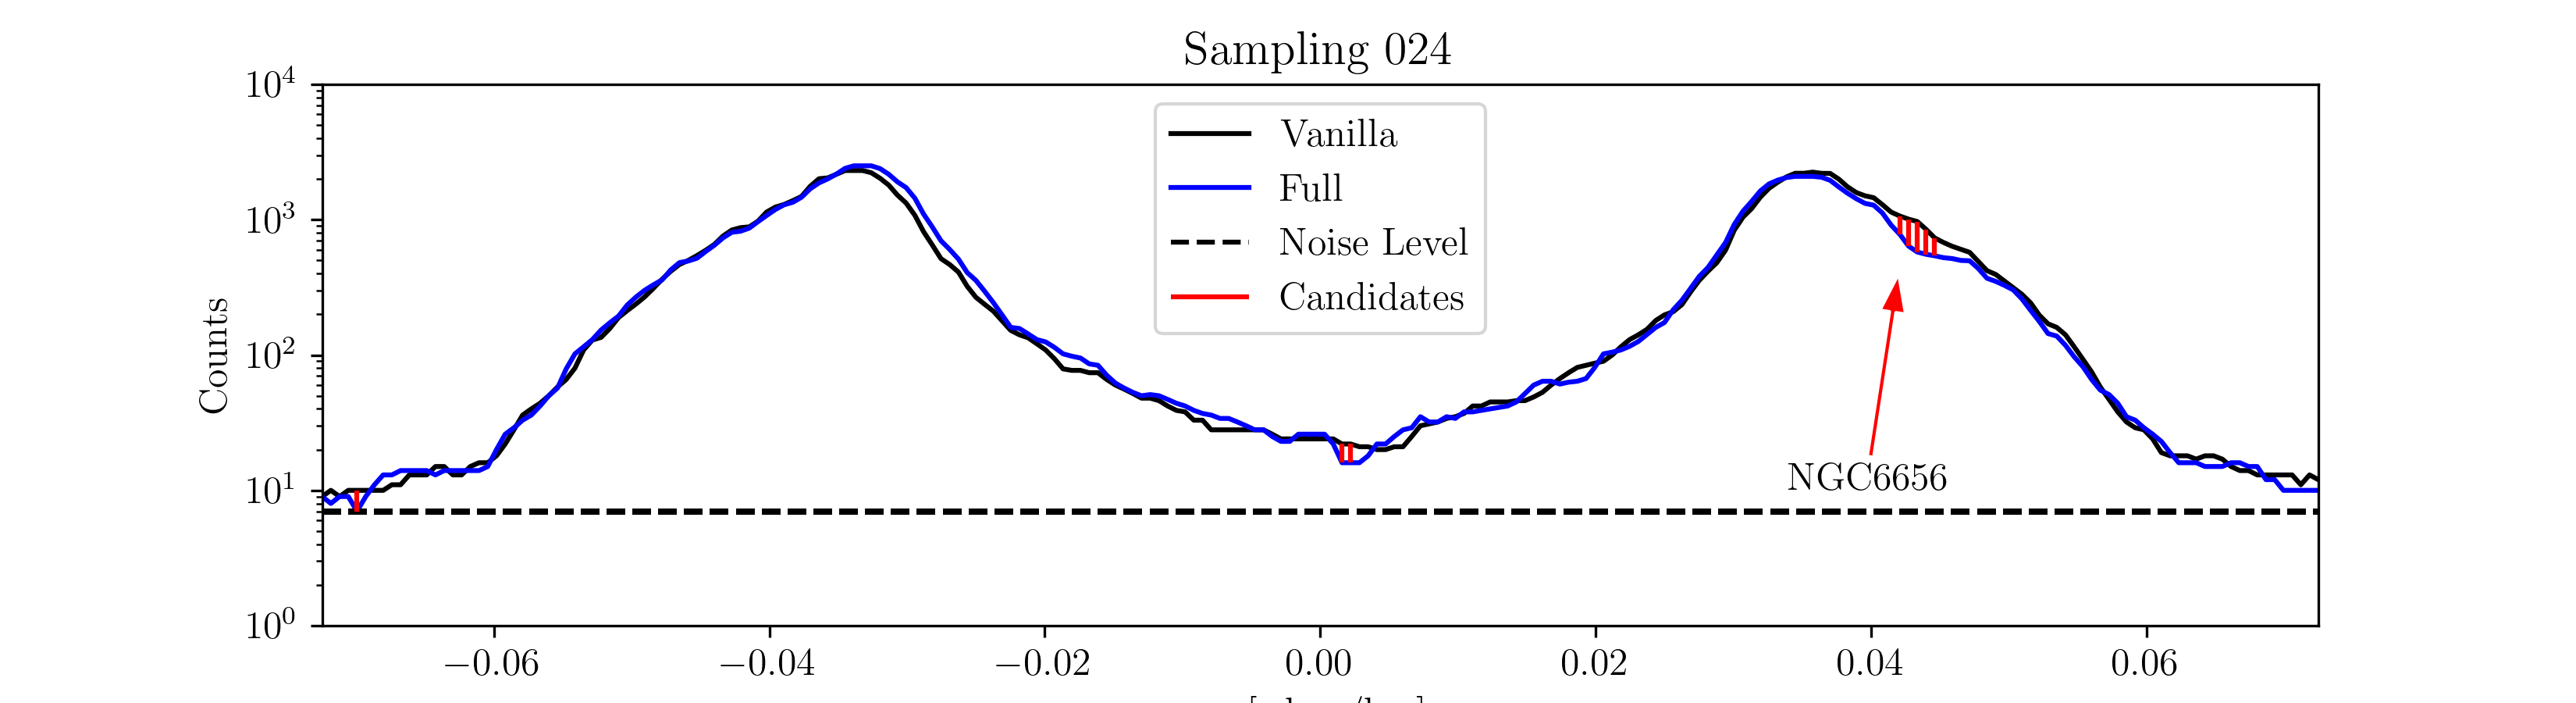
\includegraphics[width=\linewidth]{tau-profile-monte-carlo-024.png}
      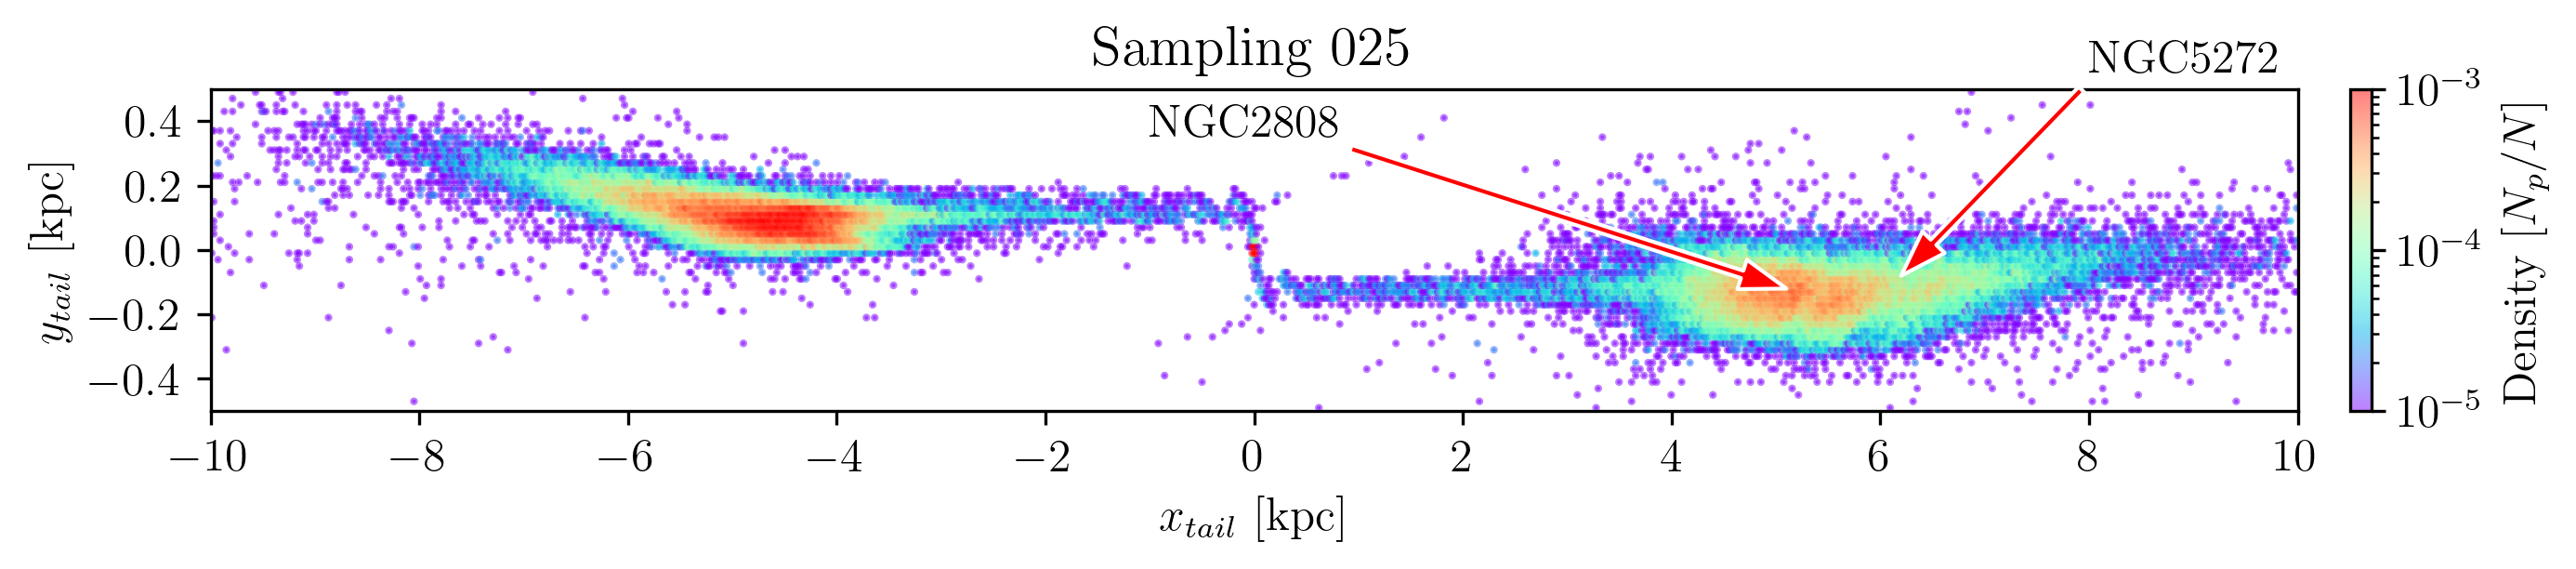
\includegraphics[width=\linewidth]{gallery_of_gaps_monte-carlo-025.png}
      \caption{Sixth gap gallery}
      \label{fig:gallery5}
      \end{figure*}        

    \begin{figure*}
      \centering
      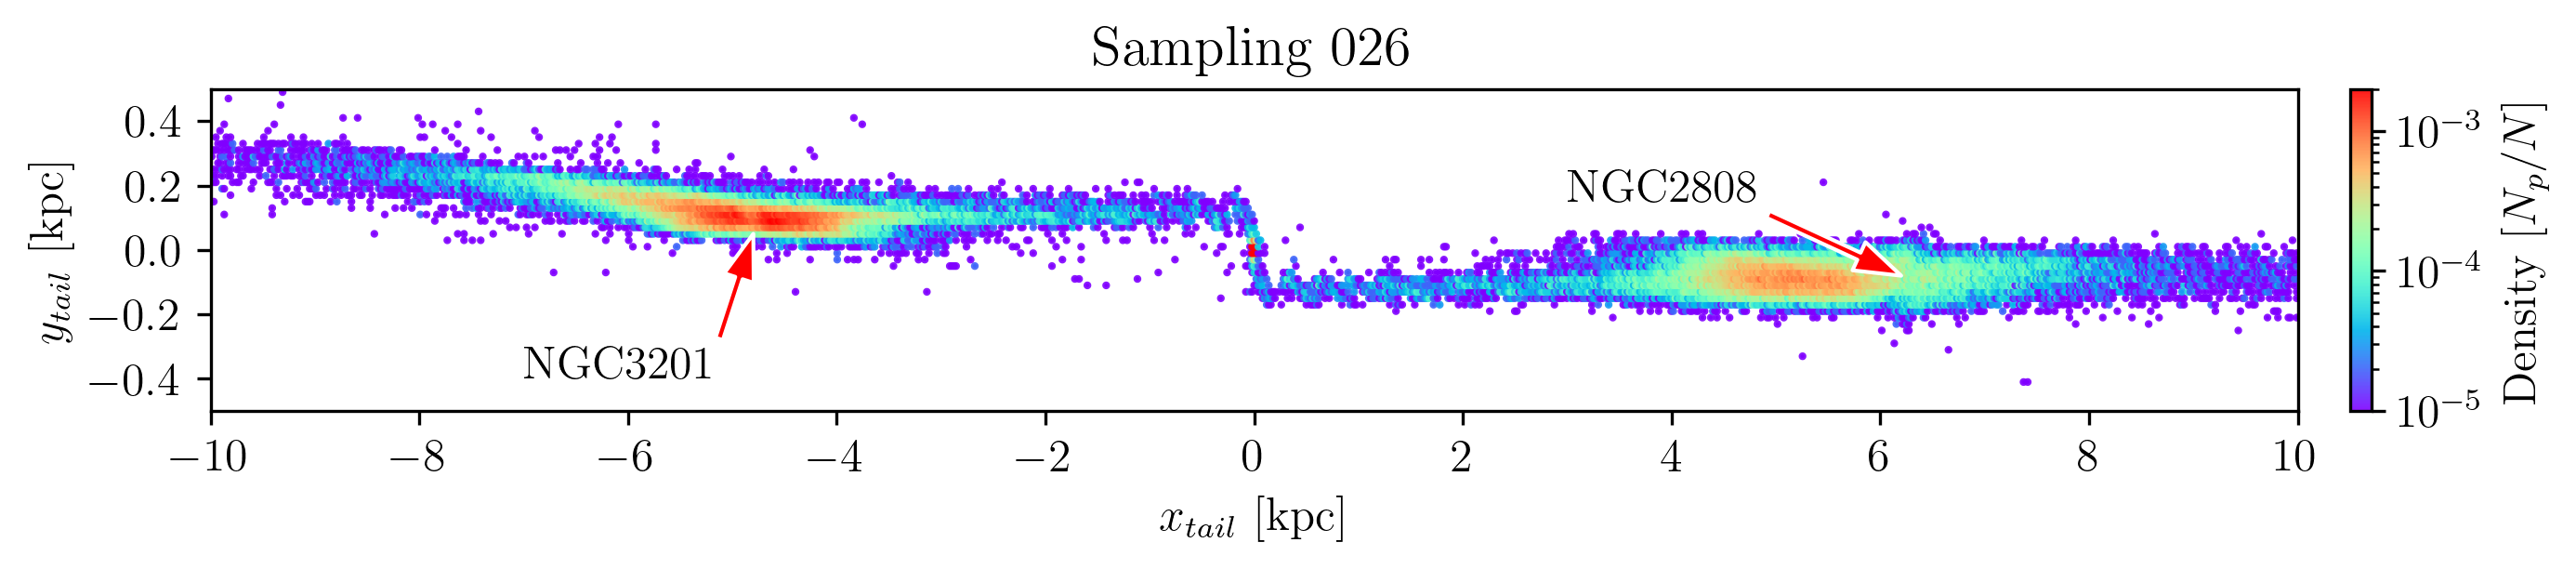
\includegraphics[width=\linewidth]{gallery_of_gaps_monte-carlo-026.png}
      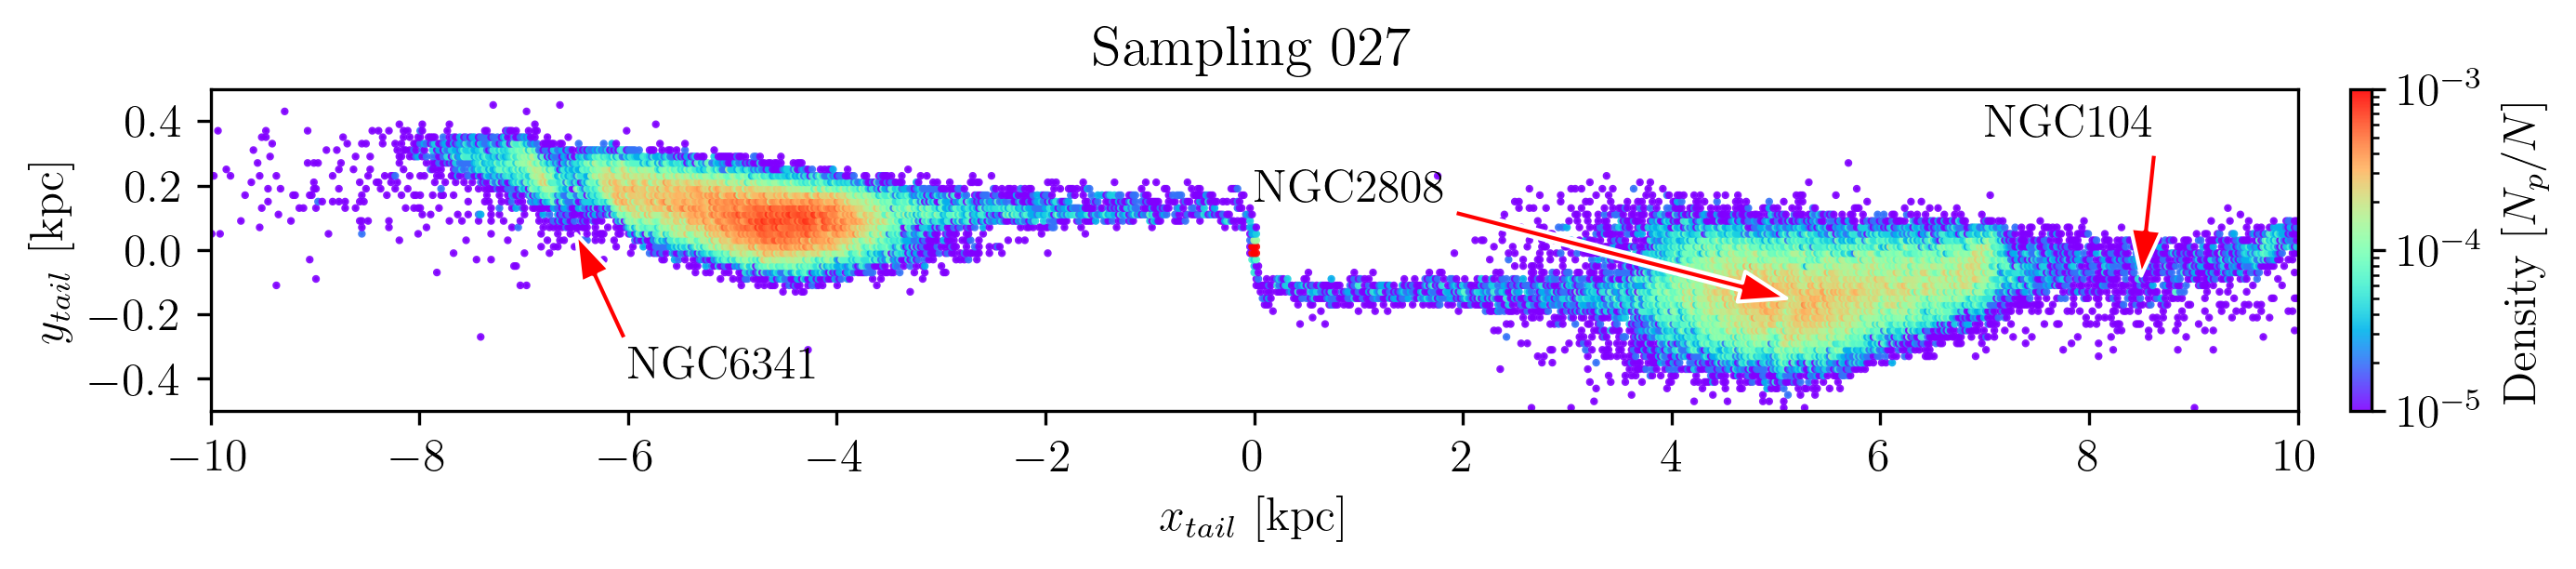
\includegraphics[width=\linewidth]{gallery_of_gaps_monte-carlo-027.png}
      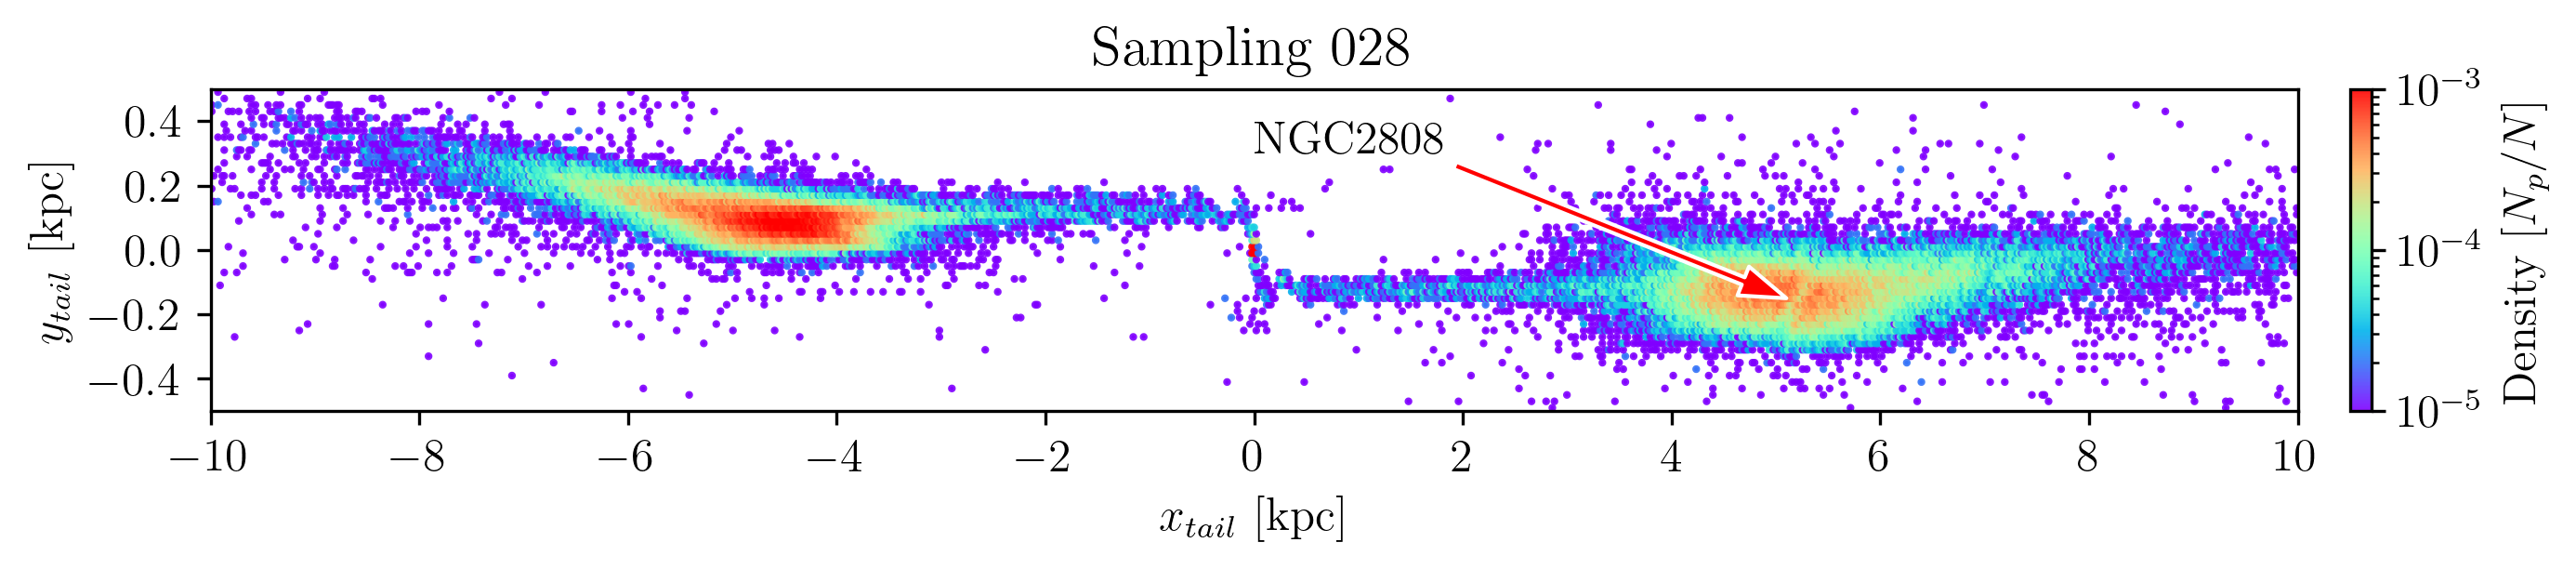
\includegraphics[width=\linewidth]{gallery_of_gaps_monte-carlo-028.png}
      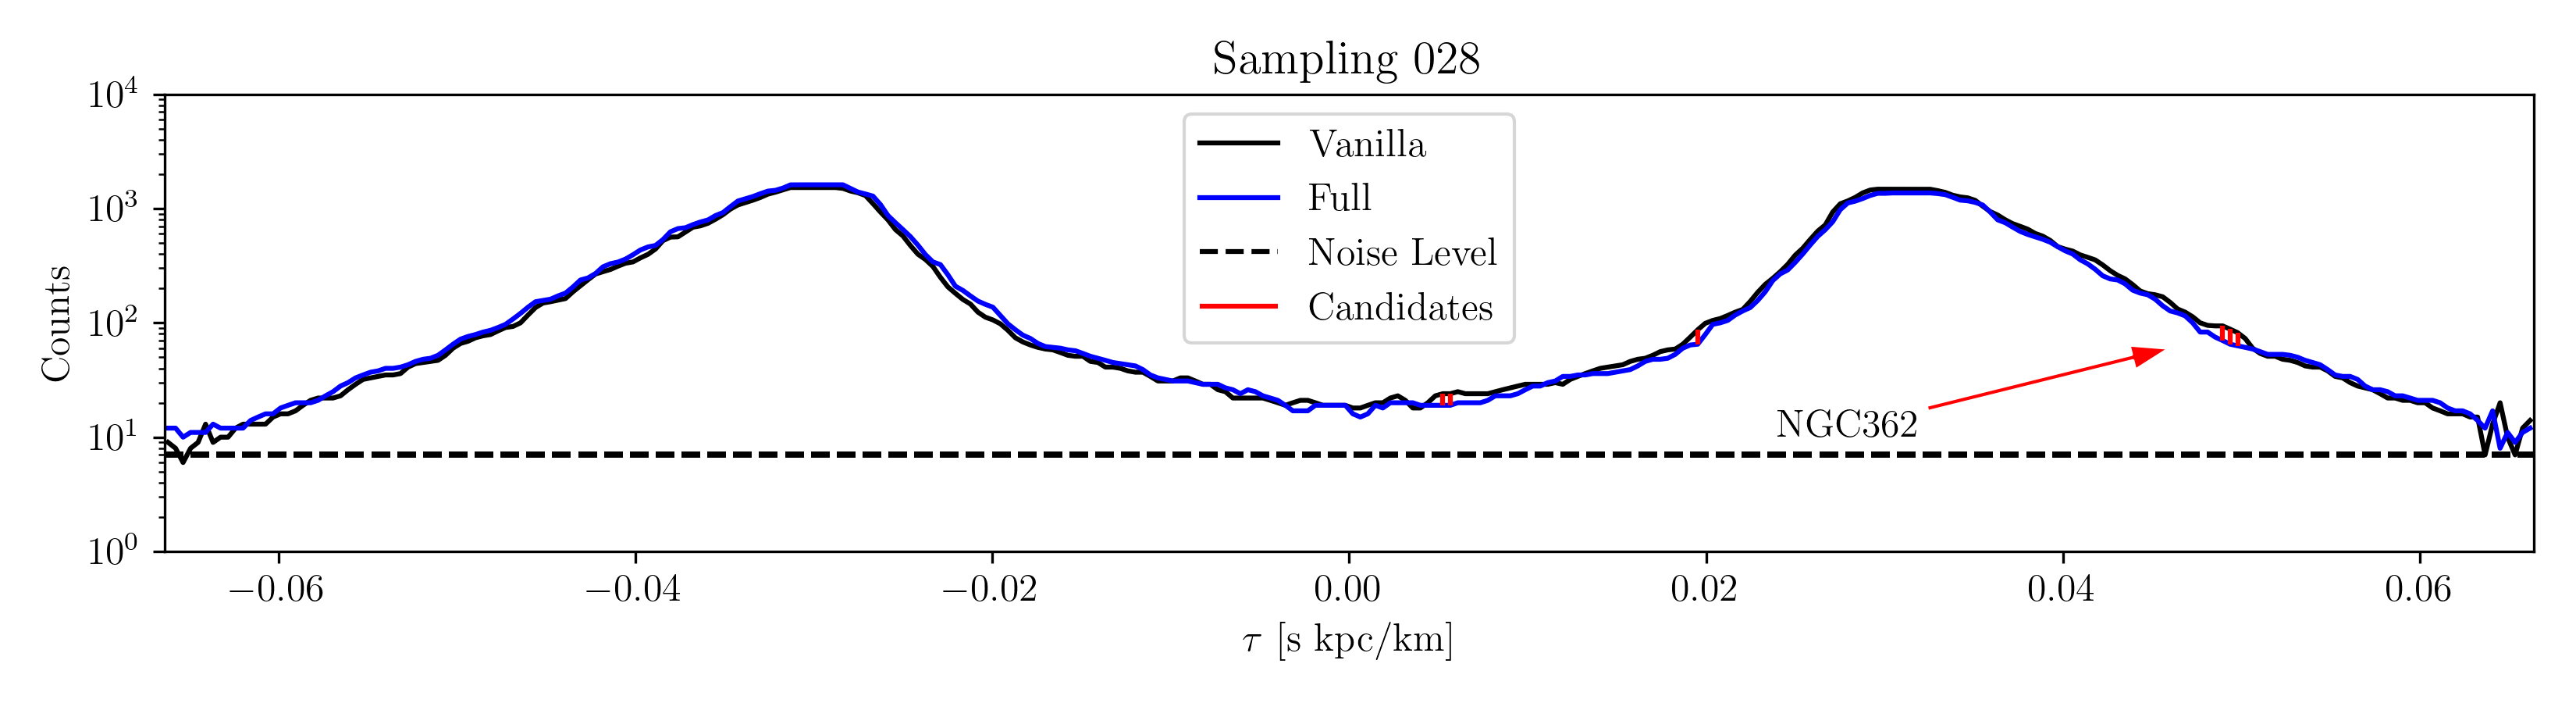
\includegraphics[width=\linewidth]{tau-profile-monte-carlo-028.png}
      \caption{Seventh gap gallery}
      \label{fig:gallery6}
      \end{figure*}        

    \begin{figure*}
      \centering      
      \includegraphics[width=\linewidth]{gallery_of_gaps_monte-carlo-029.png}    
      \includegraphics[width=\linewidth]{tau-profile-monte-carlo-029.png}  
      \includegraphics[width=\linewidth]{gallery_of_gaps_monte-carlo-030.png}
      \includegraphics[width=\linewidth]{tau-profile-monte-carlo-030.png}
      \includegraphics[width=\linewidth]{gallery_of_gaps_monte-carlo-031.png}
      \caption{Eighth gap gallery}
      \label{fig:gallery7}
      \end{figure*}        


    \begin{figure*}
      \centering
      \includegraphics[width=\linewidth]{gallery_of_gaps_monte-carlo-032.png}
      \includegraphics[width=\linewidth]{gallery_of_gaps_monte-carlo-033.png}
      \includegraphics[width=\linewidth]{gallery_of_gaps_monte-carlo-034.png}      
      \includegraphics[width=\linewidth]{gallery_of_gaps_monte-carlo-035.png}
      \includegraphics[width=\linewidth]{gallery_of_gaps_monte-carlo-036.png}      
      \caption{Ninth gap gallery}
      \label{fig:gallery8}
      \end{figure*}    



    \begin{figure*}
      \centering
      \includegraphics[width=\linewidth]{gallery_of_gaps_monte-carlo-037.png}
      \includegraphics[width=\linewidth]{gallery_of_gaps_monte-carlo-038.png}
      \includegraphics[width=\linewidth]{gallery_of_gaps_monte-carlo-039.png}
      \includegraphics[width=\linewidth]{gallery_of_gaps_monte-carlo-040.png}
      \includegraphics[width=\linewidth]{gallery_of_gaps_monte-carlo-041.png}      
      \caption{Tenth gap gallery}
      \label{fig:gallery9}
    \end{figure*}        

    \begin{figure*}
      \centering
      \includegraphics[width=\linewidth]{gallery_of_gaps_monte-carlo-042.png}
      \includegraphics[width=\linewidth]{gallery_of_gaps_monte-carlo-043.png}
      \includegraphics[width=\linewidth]{gallery_of_gaps_monte-carlo-044.png}
      \includegraphics[width=\linewidth]{tau-profile-monte-carlo-044.png}
      \includegraphics[width=\linewidth]{gallery_of_gaps_monte-carlo-045.png}
      \caption{Eleventh gap gallery}
      \label{fig:gallery010}
    \end{figure*}   

    \begin{figure*}
      \centering
      \includegraphics[width=\linewidth]{gallery_of_gaps_monte-carlo-046.png}
      \includegraphics[width=\linewidth]{gallery_of_gaps_monte-carlo-047.png}
      \includegraphics[width=\linewidth]{gallery_of_gaps_monte-carlo-048.png}
      \includegraphics[width=\linewidth]{tau-profile-monte-carlo-048.png}
      \includegraphics[width=\linewidth]{gallery_of_gaps_monte-carlo-049.png}
      \caption{Twelfth gap gallery}
      \label{fig:gallery11}
    \end{figure*} 


\end{appendix}

\end{document}